% Time-stamp: <2011-09-08 23:57 yannick@lyopc469>
% Auteurs (version LaTeX):
% Nicolas Chotard <nchotard@ipnl.in2p3.fr>
% Yannick Copin <ycopin@ipnl.in2p3.fr>
% Eric Chabanat <chabanat@ipnl.in2p3.fr>

% Compiler tel quel 'pdflatex TD_astro_L2' pour avoir les solutions,
% et compiler avec 'pdflatex
% "\def\sanscorrige{}% Time-stamp: <2011-09-08 23:57 yannick@lyopc469>
% Auteurs (version LaTeX):
% Nicolas Chotard <nchotard@ipnl.in2p3.fr>
% Yannick Copin <ycopin@ipnl.in2p3.fr>
% Eric Chabanat <chabanat@ipnl.in2p3.fr>

% Compiler tel quel 'pdflatex TD_astro_L2' pour avoir les solutions,
% et compiler avec 'pdflatex
% "\def\sanscorrige{}% Time-stamp: <2011-09-08 23:57 yannick@lyopc469>
% Auteurs (version LaTeX):
% Nicolas Chotard <nchotard@ipnl.in2p3.fr>
% Yannick Copin <ycopin@ipnl.in2p3.fr>
% Eric Chabanat <chabanat@ipnl.in2p3.fr>

% Compiler tel quel 'pdflatex TD_astro_L2' pour avoir les solutions,
% et compiler avec 'pdflatex
% "\def\sanscorrige{}% Time-stamp: <2011-09-08 23:57 yannick@lyopc469>
% Auteurs (version LaTeX):
% Nicolas Chotard <nchotard@ipnl.in2p3.fr>
% Yannick Copin <ycopin@ipnl.in2p3.fr>
% Eric Chabanat <chabanat@ipnl.in2p3.fr>

% Compiler tel quel 'pdflatex TD_astro_L2' pour avoir les solutions,
% et compiler avec 'pdflatex
% "\def\sanscorrige{}\input{TD_astro_L2}"' pour une version sans
% les solutions.

\documentclass[a4paper,10pt]{report}

% PREAMBULE ==============================

\usepackage[T1]{fontenc}
\usepackage[utf8]{inputenc}
\usepackage[ec]{aeguill}
\usepackage{ae}
\usepackage[cm]{fullpage}
\usepackage[francais]{babel}
\usepackage{amsmath}
\usepackage{multirow}

\usepackage[pdftex]{graphicx}
\graphicspath{{./Figures/}}

%\usepackage[backref,colorlinks=true,breaklinks=true,
%a4paper,bookmarks=false,linktocpage=true]{hyperref}
\usepackage[colorlinks=true]{hyperref}
\hypersetup{
  pdftitle   = Fascicule de TD,
  pdfauthor  = Astro L2,
  pdfsubject = Astrophysique,
}

% Définition de l'environnement 'Exercise'
\newcounter{noexo}
\setcounter{noexo}{0}
\newenvironment{Exercise}[1][]{%
  \stepcounter{noexo}
  \medskip\noindent\textbf{Exercice~\thenoexo~:~#1}
  \medskip\par
  \addcontentsline{toc}{subsubsection}{Exercice~\thenoexo~:~#1}
}{}

% Définition de l'environnement 'Answer'
\usepackage[usenames,dvipsnames]{color}
\usepackage{comment}
\specialcomment{Answer}{%
  \begingroup
  \sffamily\color{CadetBlue}
  \medskip\noindent\textbf{Corrigé :~}
  }{%
  \endgroup}

% Inclusion ou non des corrigés
\ifdefined\sanscorrige
  \message{Fascicule sans solutions}%
  \excludecomment{Answer} % Remove answers
\else
  \message{Fascicule *AVEC* solutions}%
\fi

% Définitions locales
\renewcommand{\d}{\ensuremath{\mathrm{d}}}
\newcommand{\UA}{\ensuremath{\textrm{UA}}}
\renewcommand{\deg}{\ensuremath{^{\circ}}}
\renewcommand{\vec}[1]{\ensuremath{\boldsymbol{#1}}}
\renewcommand{\u}[1]{\ensuremath{\mathrm{#1}}} % Unités

% PAGE DE TITRE ET PREAMBULE ==============================

\makeatletter
\def\thickhrulefill{\leavevmode \leaders \hrule height 1pt\hfill \kern \z@}
\renewcommand{\maketitle}{\begin{titlepage}%
    \let\footnotesize\small
    \let\footnoterule\relax
    \parindent \z@
    \reset@font
    \null
    \begin{center}
      \huge \bfseries \@title
      \ifdefined\sanscorrige
      \else
      \\\textcolor{red}{avec solutions}
      \fi
    \end{center}
    \hrule height 1pt
    \begin{flushright}
      Université Claude Bernard Lyon1 \\
    \end{flushright}
    \vfil
    \vfil
    \begin{figure}[htp]
      \centering
      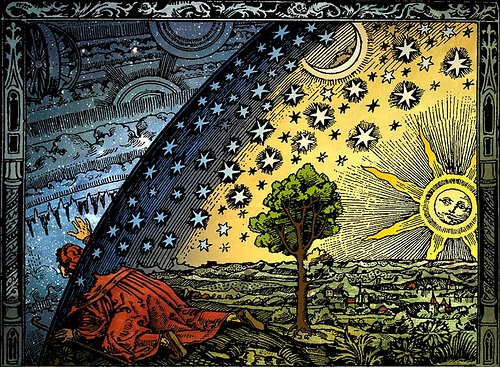
\includegraphics[width=0.8\textwidth]{flammarion}
      \caption{La gravure sur bois dite « de Flammarion »}
    \end{figure}
    \begin{center}
    \vfil
      {\Large \@author} \\[1em]
      {\large \@date}
    \end{center}
  \end{titlepage}%
  \setcounter{footnote}{0}%
}
\makeatother

\title{Fascicule de TD}
\date{Université Lyon 1}
\author{Astrophysique pour la licence}

\begin{document}

\maketitle

% 2: Down to subsection (no exercices)
% 3: Down to subsubsection (exercices)
\setcounter{tocdepth}{2}
\tableofcontents

\newpage

% EXERCICES ET SOLUTIONS ==============================

\chapter{Vie des étoiles}

\section{La lumière des étoiles}

\subsection{Notion de photométrie}

\begin{Exercise}[Dilution du flux avec la distance]
  Réécrire la relation entre la luminosité d'une étoile et le flux
  observé (équation 2.4) dans le cas où la luminosité $L(t)$ dépend du
  temps (par exemple parce que l'étoile est variable) et donc le flux
  observé $F(D,t)$ dépend du temps et de la distance.
\end{Exercise}

\begin{Answer}
  Lorsque la luminosité $L(t)$ de l'étoile dépend du temps, les
  variations de luminosité mettent un temps $D/c$ pour parvenir à un
  observateur situé à une distance $D$ ($c$ étant la vitesse de la
  lumière). Dans ce cas la relation (2.4) devient: $L(t) = 4 \pi D^2
  F(D,t-D/c) $.
\end{Answer}

\subsection{Photosphère et température effective}

\begin{Exercise}[Température effective d'une étoile]
  Calculer la température effective du Soleil à partir de sa
  luminosité $L_{\odot}\approx 3.83\times 10^{26}$~W et de son rayon
  $R_{\odot}\approx 6.96 \times 10 ^{8}$~m.
\end{Exercise}

\begin{Answer}
  En appliquant l'équation :
  $$
  T_e = \left( \frac{L}{4 \pi \sigma R^2_p} \right)^{1/4}
  $$
  avec la constante de Stefan $\sigma = 5.67 \times
  10^{-8}$~\u{Wm^{-2}K^{-4}}, on trouve la température effective du
  Soleil $T_\odot \approx 5770$~K.
\end{Answer}

\subsection{Système de magnitudes}

\begin{Exercise}[Indices de couleur]
  Les deux composantes de l'étoile $\alpha$ du Centaure située à
  1,32~pc de distance ont des magnitudes visuelles (magnitude
  apparente dans la bande $V$) de 0,30 et 1,70. On demande :
  \begin{enumerate}
  \item Le rapport des flux des deux étoiles dans la bande $V$.
  \item La magnitude visuelle globale du système.
  \item La correction qu'il faut apporter aux magnitudes apparentes de
    ce système pour obtenir les magnitudes absolues.
  \end{enumerate}
\end{Exercise}

\begin{Answer}
  On rappelle que la magnitude apparente $m$ est liée au flux $F$ par
  $m = -2,5 \log_{10}(F / F_{0})$.
  \begin{enumerate}
  \item Le rapport des flux des deux composantes de $\alpha$ du
    Centaure dépend de la différence de magnitudes et vaut :
    $$
    F_2 / F_1 = 10^{(m_{1} - m_{2})/2,5} = 0,28
    $$
  \item Pour obtenir la magnitude visuelle globale du système $m_{tot}$,
    il faut calculer le flux total (les puissances émises par les deux
    composantes s'ajoutent) :
    $$
    m_{tot} = -2,5 \log(F_{1} / F_{0} + F_{2} / F_{0})
    $$
    donc
    $$
    m_{tot}= -2,5 \log(10^{-m_{1}/2,5} + 10^{-m_{2}/2,5}) = 0.04
    $$
  \item La correction qu'il faut apporter aux magnitudes apparentes
    $m$ de ce système pour obtenir les magnitudes absolues $M$ vaut:
    $$
    m - M = 5 \log(D/10 \u{pc}) = -4,4
    $$
  \end{enumerate}
\end{Answer}

\section{Évolution stellaire}

\subsection{Formation des étoiles}

\begin{Exercise}
  Quelle est la source de l'énergie rayonnée par:
  \begin{enumerate}
  \item une proto-étoile?
  \item une étoile?
  \item une naine brune?
  \end{enumerate}
\end{Exercise}

\begin{Answer}
  L'énergie rayonnée provient de:
  \begin{enumerate}
  \item l'énergie gravitationnelle pour une proto-étoile ;
  \item l'énergie produite par les réactions nucléaires pour une
    étoile (fusion de H sur la séquence principale, fusion de He ou de
    C et O ensuite, selon la masse de l'étoile) ;
  \item l'énergie gravitationnelle pour une naine brune, qui continue
    à se contracter, ne passant jamais de la proto-étoile à l'étoile.
  \end{enumerate}
\end{Answer}

\subsection{Séquence principale}

\begin{Exercise}
  Quel est le phénomène marquant:
  \begin{enumerate}
  \item le début de la séquence principale?
  \item sa fin?
  \end{enumerate}
\end{Exercise}

\begin{Answer}
  La séquence principale débute quand les réactions de fusion de
  l'hydrogène s'allument dans le coeur de la proto-étoile, et se
  termine lorsque la fusion de l'hydrogène cesse au centre (elle peut
  continuer dans une couche autour d'un noyau d'hélium ou cesser dans
  toute l'étoile selon sa masse).
\end{Answer}

\subsection{Évolution post-SP}

\begin{Exercise}[Étoile de $M > 5 M_{\odot}$]
  Que se passe-t-il si un combustible s'épuise au centre d'une étoile?
\end{Exercise}

\begin{Answer}
  Quand un combustible s'épuise au centre d'une étoile, les réactions
  de fusion de cet élément cessent dans le coeur, mais peuvent
  continuer autour, dans une couche où le combustible est toujours
  présent. Au centre, il n'y a plus de production d'énergie pour
  soutenir le coeur, la gravité l'emporte et le coeur se
  contracte. Cette contraction provoque une augmentation de
  température qui, si elle est suffisante (cela dépend de la masse de
  l'étoile), permet d'allumer de nouvelles réactions nucléaires ayant
  pour combustible le produit des réactions précédentes.
\end{Answer}

\section{Classification spectrale}

\subsection{Mesures des distances}

\subsubsection{Parallaxe trigonométrique}

\begin{Exercise}
  Relier l'incertitude sur la distance $\Delta d$ à celle sur la
  parallaxe $\Delta p$.
\end{Exercise}

\begin{Answer}
  Il existe deux méthodes pour trouver le résultat demandé:
  \begin{itemize}
  \item En différenciant l'équation $d = a/p$, on obtient $\d d =
    -(a/p^2)\d p$, d'où l'incertitude en prenant la valeur absolue:
    $$
    \Delta d = \frac{a}{p^2}\Delta p = \frac{d}{p}\Delta p
    $$
    On a finalement
    $$
    \frac{\Delta d}{d} = \frac{\Delta p}{p}
    $$

  \item On peut également prendre le logarithme de l'équation $d =
    a/p$, ce qui donne $\ln~d = \ln~a - \ln~p$, puis on différencie:
    $\d\ln~d = -\d\ln~p$, soit $\d d/d = -\d p/p$. En prenant la
    valeur absolue, on retrouve le résultat sur l'incertitude:
    $$
    \frac{\Delta d}{d} = \frac{\Delta p}{p}
    $$
  \end{itemize}
\end{Answer}

\begin{Exercise}
  Imaginons deux missions spatiales: FAME et GAIA. Quelles seraient
  les précisions obtenues à une distance de 100~pc? de 1000~pc?  À
  quelle distance aura-t-on une erreur de 100\%?

  On donne les incertitudes absolues sur les parallaxes pour chaque
  satellite:
  \begin{itemize}
  \item $\Delta p=50~\mu as$ pour FAME et
  \item $\Delta p=4~\mu as$ pour GAIA.
  \end{itemize}
\end{Exercise}

\begin{Answer}
  Les étoiles situées à $d=100$~pc ont une parallaxe
  $p=1/100=0,01''=10$~mas. La précision obtenue avec FAME sera de
  $$
  \frac{\Delta d}{d} = \frac{\Delta p}{p} = \frac{50 \times
    10^{-6}}{10^{-2}} = 5 \times 10^{-3} = 0.5 \%
  $$
  et de
  $$
  \frac{\Delta d}{d} = \frac{\Delta p}{p} = \frac{4 \times
    10^{-6}}{10^{-2}} = 4 \times 10^{-4} = 0.04 \%
  $$
  avec GAIA.

  Pour des étoiles à $d=1000$~pc, $p=1$~mas, et les précisions
  deviennent 10 fois moins bonnes: 5\% avec FAME et 0,4\% avec GAIA.

  On aura une erreur de 100\% quand $\Delta d =d$, soit $\delta p =
  p$. La distance correspondante s'obtient donc par
  $$
  d = \frac{1}{p} = \frac{1}{50 \times 10^{-6}} = 20~\u{kpc}
  \quad\text{avec FAME}
  $$
  et
  $$
  d = \frac{1}{p} = \frac{1}{4 \times 10^{-6}} = 250~\u{kpc}
  \quad\text{avec GAIA}
  $$
\end{Answer}


\begin{Exercise}
  Le tableau suivant donne la magnitude apparente $m_V$ et la
  parallaxe $p$ de trois étoiles. Calculer leur distance $d$ avec son
  incertitude, l'erreur relative sur la distance $\Delta d / d$ et
  leur magnitude absolue $M_V$.
  \begin{center}
    \begin{tabular}{|c|c|c|c|}
      \hline
      & $\alpha$ CMa Sirius & $\alpha$ Tau Aldebaran & $\alpha$ Ori
      Bételgeuse \\
      \hline
      $m_V$ & -1.47 & 0.85 & 0.58 \\
      \hline
      $p$ (mas) & 379.2 $\pm$ 1.6 & 50.1 $\pm$ 1.0 & 7.6 $\pm$ 1.6 \\
      \hline
      $d$ (pc) &   &   &  \\
      \hline
      $\Delta d / d$ &   &   &  \\
      \hline
      $M_V$ &   &   &  \\
      \hline
    \end{tabular}
  \end{center}
\end{Exercise}

\begin{Answer}
  \begin{center}
    \begin{tabular}{|c|c|c|c|}
      \hline
      & $\alpha$ CMa Sirius & $\alpha$ Tau Aldebaran & $\alpha$ Ori
      Bételgeuse \\
      \hline
      $m_V$ & -1.47 & 0.85 & 0.58 \\
      \hline
      $p$ (mas) & 379.2 $\pm$ 1.6 & 50.1 $\pm$ 1.0 & 7.6 $\pm$ 1.6 \\
      \hline
      $d$ (pc) &  \color{red}{2.64 $\pm$ 0.01} &  \color{red}{20.0
        $\pm$ 0.4}  & \color{red}{130 $\pm$ 30} \\
      \hline
      $\Delta d / d$ & \color{red}{0.4\%}  & \color{red}{2\%}  &
      \color{red}{23\%} \\
      \hline
      $M_V$ & \color{red}{1.42}  & \color{red}{-0.65}  &
      \color{red}{-4.99} \\
      \hline
    \end{tabular}
  \end{center}

  Étant donné la forme de la relation donnant la distance $d$ à partir
  de la parallaxe $p$, leurs incertitudes relatives sont égales, ce
  qui permet d'avoir immédiatement $\Delta d / d$. Ces résultats
  illustrent bien la diminution de la précision lorsque la distance
  augmente.

  La magnitude absolue s'obtient par la relation $M_V = m_V - 5~\log~d
  + 5$.
\end{Answer}


\begin{Exercise}[Méthode du point convergent]
  On veut déterminer la distance de l'amas des Pléiades par la méthode
  du point convergent.
  \begin{itemize}
  \item L'étude des trajectoires des étoiles de l'amas sur plusieurs
    années a permis de situer le point convergent à $\theta = 67,9 \pm
    0,6\deg$ de la direction de l'amas.
  \item L'observation du spectre de l'étoile Alcyone, faisant partie
    de cet amas, a permis de mesurer sa vitesse radiale $v_r = 10,1
    \pm 0,3$~\u{km.s^{-1}}.
  \item Le mouvement propre apparent de cette même étoile vaut $\mu =
    47,3 \pm 0,8$~\u{mas.an^{-1}}.
  \end{itemize}
  Déterminer la distance de l'amas. Attention aux unités !
\end{Exercise}

\begin{Answer}
  Dans la formule donnant la distance de l'amas, il faut bien faire
  attention à exprimer l'angle $\mu$ en radians et à utiliser les
  mêmes unités de distance et de temps pour les autres grandeurs.
  \begin{itemize}
  \item $\mu = 47,3 \pm 0,8~\u{mas.an^{-1}} = (2,29 \pm 0,04) \times
    10^{-7}~\u{rad.an^{-1}}$
  \item $v_r = 10,1 \pm 0,3~\u{km.s^{-1}} = (1,02 \pm 0,03) \times
    10^{-5}~\u{pc.an^{-1}}$
  \item $\theta = 67,9 \pm 0,6\deg = 1,19 \pm 0,01$~rad
  \item On a donc $tan \theta= 2,50 \pm 0,07$.
  \item Finalement: $d = 111 \pm 8$~pc
  \end{itemize}
\end{Answer}

\subsection{Classification stellaire}

\begin{Exercise}[Types spectraux]
  Donner approximativement le type spectral des étoiles dont le flux
  est maximal aux longueurs d'onde suivantes: 300~nm, 500~nm, et
  1,2~$\mu$m.  Peut-on déterminer la classe de luminosité?

  Rappel de la loi de Wien: $\lambda_{\max} T = 2898$~\u{\mu m.K}.
\end{Exercise}

\begin{Answer}
  La loi de Wien permet de déterminer la température effective de
  chaque étoile, et ainsi d'en déduire une valeur approximative du
  type spectral. Ici seulement la première lettre est accessible, la
  détermination du chiffre suivant nécessiterait un tableau plus
  précis donnant les correspondances entre les sous-types et la
  température effective.
  \begin{center}
    \begin{tabular}{|c|c|c|}
      \hline
      $\lambda_m$ & $T_{eff}(K)$ & Type spectral \\
      \hline
      300 nm & \color{red}{9660} & \color{red}{A}  \\
      \hline
      500 nm & \color{red}{5796} & \color{red}{G} \\
      \hline
      1.2 $\mu m$ &  \color{red}{2415} &  \color{red}{M} \\
      \hline
    \end{tabular}
  \end{center}
  On ne peut pas déterminer la classe de luminosité grâce à la
  longueur d'onde du maximum du flux. Pour ceci, il faudrait connaître
  soit la luminosité de l'étoile, soit sa gravité de surface, soit son
  rayon.
\end{Answer}

\begin{Exercise}[Diagramme HR]
  Classer par ordre de température effective croissante, puis de rayon
  croissant, et enfin de luminosité croissante les étoiles de types
  spectraux suivants: M5III, O2V, K7I, A0VII.
\end{Exercise}

\begin{Answer}
  La séquence OBAFGKM décrit les types spectraux dans le sens des
  $T_{eff}$ décroissantes, on aura donc dans le sens des $T_{eff}$
  croissantes: \textcolor{red}{M5III}, \textcolor{red}{K7I},
  \textcolor{red}{A0VII}, et \textcolor{red}{O2V}.

  La classe de luminosité définit des groupes d'étoiles de rayon
  différent, on aura donc dans l'ordre croissant:
  \textcolor{red}{A0VII}, \textcolor{red}{O2V},
  \textcolor{red}{M5III}, et \textcolor{red}{K7I}.

  Enfin, l'examen du diagramme HR montre qu'une étoile chaude de la
  séquence principale peut être plus lumineuse qu'une sous-géante
  froide, et on aura dans le sens des luminosités croissantes:
  \textcolor{red}{A0VII}, \textcolor{red}{M5III},
  \textcolor{red}{O2V}, et \textcolor{red}{K7I}.

  Ceci montre que le terme « classe de luminosité » peut être source
  d'erreur.
\end{Answer}

\subsection{Mesure des rayons}

\begin{Exercise}[Interférométrie]
  Le tableau suivant donne le diamètre apparent $\theta_*$ de quelques
  étoiles, mesuré par interférométrie. Calculer leur rayon $R$ (on
  rappelle les distances déterminées dans un exercice précédent) et, à
  l'aide de ce résultat, attribuer à chaque étoile sa classe de
  luminosité parmi les suivantes: I, III, V.

  \begin{center}
    \begin{tabular}{|c|c|c|c|}
      \hline
      & $\alpha$ CMa Sirius & $\alpha$ Tau Aldebaran & $\alpha$ Ori
      Bételgeuse \\
      \hline
      $\theta_*$ (mas) & 5.89 & 24 & 67 \\
      \hline
      $p$ (mas) & 379.2 $\pm$ 1.6 & 50.1 $\pm$ 1.0 & 7.6 $\pm$ 1.6 \\
      \hline
      $d$ (pc) & 2.64  & 20  & 130 \\
      \hline
      $R (R_{\odot})$ &   &   &  \\
      \hline
      Classe de luminosité &   &   &  \\
      \hline
    \end{tabular}
  \end{center}
\end{Exercise}

\begin{Answer}
  Pour Sirius:
  \begin{itemize}
  \item Son diamètre apparent vaut $\theta_*= 5,89~\u{mas} = 2,86 \times
    10^{-8}$~rad.
  \item Son rayon vaut donc $R = \theta_* d / 2 = 3,8 \times 10^{-8}
    pc = 1,2 \times 10^9 m = 1,7R_{\odot}$.
  \end{itemize}
  Le tableau suivant donne les résultats pour les 3 étoiles:
  \begin{center}
    \begin{tabular}{|c|c|c|c|}
      \hline
      & $\alpha$ CMa Sirius & $\alpha$ Tau Aldebaran & $\alpha$ Ori
      Bételgeuse \\
      \hline
      $\theta_*$ (mas) & 5.89 & 24 & 67 \\
      \hline
      $p$ (mas) & 379.2 $\pm$ 1.6 & 50.1 $\pm$ 1.0 & 7.6 $\pm$ 1.6 \\
      \hline
      $d$ (pc) & 2.64  & 20  & 130 \\
      \hline
      $R (R_{\odot})$ & \color{red}{1.7}  & \color{red}{52}  &
      \color{red}{936} \\
      \hline
      Classe de luminosité & \color{red}{V}  & \color{red}{III}  &
      \color{red}{I} \\
      \hline
      Type spectral & A1V  & K5III  & M2I \\
      \hline
    \end{tabular}
  \end{center}
  Dans cet exemple, il est possible d'attribuer à chaque étoile sa
  classe de luminosité en utilisant le lien qui existe avec le rayon
  stellaire. Le type spectral complet est donné pour information.
\end{Answer}

\subsection{Mesure de masse}

\subsubsection{Étoiles doubles}

\begin{Exercise}
  On observe une étoile double visuelle dont le plan de l'orbite est
  perpendiculaire à la ligne de visée.
  \begin{itemize}
  \item La parallaxe de ce système est de 100~mas.
  \item La plus grande séparation angulaire entre les deux composantes
    est de $5''$, et la plus petite de $1''$.
  \item La période de révolution est de 30~ans.
  \item L'étoile primaire se trouve au foyer de l'orbite observée, car
    il n'y a pas d'effet de projection.
  \item Le compagnon est toujours observé à une distance du centre de
    gravité 5~fois plus grande que celle de l'étoile primaire.
  \end{itemize}

  Déterminer la masse de chaque composante.
\end{Exercise}

\begin{Answer}
  Les paramètres observés permettent de remonter aux données suivantes
  pour le système:
  \begin{itemize}
  \item La distance est $d = 10$~pc.
  \item La dimension angulaire du grand axe de l'orbite relative est
    de $5'' + 1'' = 6''$. Le demi-grand axe apparent est donc $\theta
    = 3''$, soit $\theta = 1,45 \times 10^{-5} rad$.
  \item Le demi-grand axe de l'orbite relative vaut donc $a = \theta d
    = 1,45 \times 10^{-4} pc = 4,49 \times 10^{12} m = 30 \UA$.
  \item La $3^{ème}$ loi de Kepler donne la somme des masses: $M1 + M2
    = 5,97 \times 10^{31} kg = 30 M_{\odot}$ .
  \item Les distances des étoiles $E_1$ et $E_2$ au centre de gravité
    $G$ vérifient $M_1 \times GE_1 = M_2 \times GE_2$. Le rapport des
    masses vaut donc $M_1 / M_2 = GE_2 / GE_1 = 5$.
  \item Finalement: $M_1 = 25M_{\odot}$ et $M_2 = 5M_{\odot}$
  \end{itemize}
\end{Answer}


\begin{Exercise}
  Le tableau suivant rappelle les caractéristiques du système binaire
  à éclipse d'Algol ($\beta$ Per):
  \begin{center}
    \begin{tabular}{|l|c|r|}
      \hline
      $p$ (mas) &  \multicolumn{2}{c|}{35.1 $\pm$ 0.9} \\
      \hline
      $d$ (pc) & \multicolumn{2}{c|}{28.6 $\pm$ 0.7} \\
      \hline
      $T$ (jours) & \multicolumn{2}{c|}{2.8674} \\
      \hline
      & A & B \\
      \cline{1-3}
      Type spectral & B8V & K2IV \\
      \hline
      R ($R_{\odot}$) & 2.74 & 3.60 \\
      \hline
    \end{tabular}
  \end{center}
  On a mesuré de plus les paramètres orbitaux suivants (on supposera
  l'orbite circulaire, ainsi le demi-grand axe de l'ellipse projetée
  est égal au rayon de l'orbite):
  \begin{center}
    \begin{tabular}{|c|c|}
      \hline
      $\theta$ (mas) & 2.283 \\
      \hline
      $\theta_2$ (pc) & 1.872 \\
      \hline
    \end{tabular}
  \end{center}
  Quelle est la séparation des deux étoiles en km? en UA? en
  $R_{\odot}$? Comparez-la à leurs rayons.

  Quelle est la masse de chacune des étoiles?
\end{Exercise}

\begin{Answer}
  \begin{itemize}
  \item Le demi-grand axe apparent de l'orbite relative est $\theta =
    2.283~mas = 1,11 \times 10^{-8}~rad$.
  \item Le demi-grand axe de l'orbite relative vaut donc $a = \theta d
    = 3,17 \times 10^{-7}~pc = 9,77 \times 10^9~m = 0,065~\UA =
    14R_{\odot}$.
  \item La 3ème loi de Kepler donne la somme des masses:
    $M_1+M_2 = 4\pi^2 a^3/GT^2 = 8,98 \times 10^{30}~kg =
    4,52M_{\odot}$.
  \item Le rapport des demi-grands axes apparents de l'orbite relative
    $\theta$ et de l'orbite absolue de l'étoile secondaire $\theta_2$
    donne le rapport des masses: $\theta_2 / \theta = a_2 / a = M_1 /
    (M_1 + M_2) = 0,82$
  \item On obtient donc les masses $M_1 = 3,71$ et $M_2 = 0,81$.
  \end{itemize}

  Le tableau suivant récapitule les données physiques du système:
  \begin{center}
    \begin{tabular}{|l|c|r|}
      \hline
      $d$ (pc) & \multicolumn{2}{c|}{28.6 $\pm$ 0.7} \\
      \hline
      $T$ (jours) & \multicolumn{2}{c|}{2.8674} \\
      \hline
      $a$ ($R_{\odot}$) &  \multicolumn{2}{c|}{\color{red}{14}} \\
      \hline
      & A & B \\
      \cline{1-3}
      Type spectral & B8V & K2IV \\
      \hline
      R ($R_{\odot}$) & 2.74 & 3.60 \\
      \hline
      M ($M_{\odot}$) & \color{red}{3.71} & \color{red}{0.81} \\
      \hline
    \end{tabular}
  \end{center}
  On remarque que l'étoile la plus grosse (B) est la moins massive et
  la moins chaude, on peut en déduire que le minimum principal a lieu
  lorsque cette dernière occulte l'étoile A, plus chaude et plus
  lumineuse.

  On constate également que la séparation des étoiles vaut un peu
  moins de 4 fois le rayon de la plus grosse, il s'agit donc d'une
  binaire serrée.
\end{Answer}

\section{Les systèmes planétaires}

\subsection{Les lois de Kepler}

\begin{Exercise}[Enoncé et rappels sur les ellipses]
  L'orbite de Pluton est très excentrique ($e=0,248$). Son demi grand
  axe vaut 39,43~unités astronomiques (L'unité astronomique est
  définie comme le demi grand axe de l'orbite de la Terre). Montrer
  que Pluton peut être plus proche du Soleil que Neptune dont le demi
  grand axe de l'orbite vaut 30,06~UA et l'excentricité 0,009.
\end{Exercise}

\begin{Answer}
  On calcule simplement les distances planète-Soleil pour les deux
  planètes à leur périhélie et à leur aphélie. Si Neptune est repérée
  par le vecteur $\vec{SN}$ et Pluton par le vecteur $\vec{SP}$, on a:
  \begin{itemize}
  \item Au périhélie:
    $$
    SN = a_n(1-e_n) = 30.06 \times (1-0.009) = 29.79~\UA
    $$
    $$
    SP = a_p(1-e_p) = 39.43 \times (1-0.248) = 29.65~\UA
    $$
  \item À l'aphélie:
    $$
    SN = a_n(1+e_n) = 30.06 \times (1+0.009) = 30.33~\UA
    $$
    $$
    SP = a_p(1+e_p) = 39.43 \times (1+0.248) = 49.21~\UA
    $$
  \end{itemize}
  On voit que, du fait de la très grande excentricité de son orbite,
  Pluton, à son périhélie, est plus proche que Neptune du Soleil.
\end{Answer}

\begin{Exercise}[Dérivation des lois de Kepler]
  Montrer que la vitesse angulaire d'un objet décrivant une orbite
  elliptique autour du Soleil augmente lorsqu'il s'en
  rapproche. Montrer que le rapport des vitesses au périhélie (point
  le plus proche du Soleil) et à l'aphélie (point le plus éloigné du
  Soleil) ne dépend que de l'excentricité de l'orbite.  Calculer ce
  rapport pour la Terre dont l'excentricité de l'orbite vaut 0,0167,
  puis pour la comète de Halley dont l'excentricité de l'orbite vaut
  0,97.
\end{Exercise}

\begin{Answer}
  \begin{enumerate}
  \item On a vu que $r^2\dot{\theta}$ est une constante. On a donc
    $\dot{\theta}=C/r^3$ et la vitesse angulaire augmente lorsque $r$
    diminue.

  \item L'expression de la vitesse est: $\vec{v} = \dot{r}\vec{i} +
    r\dot{\theta}\vec{j}$

    Le périhélie et l'aphélie correspondent à des extremum sur la
    trajectoire, c'est à dire que $\d r/\d\theta =0$ et donc,
    puisque $\dot{r} = \dot{\theta}~\d r/\d\theta$,
    $\dot{r}=0$. La vitesse s'écrit donc bien $v = r\dot{\theta}$

  \item Puisque $r^2\dot{\theta}=C$ et que $v = r\dot{\theta}$, on a
    $v = C/r$. En reprenant les résultats vus précédemment sur les
    ellipses, on trouve $r = a(1-e)$ au périhélie, et $r = a(1+e)$ à
    l'aphélie. Le rapport des vitesse $v_p$ au périhélie et $v_a$ à
    l'aphélie est donc:
    $$
    \frac{v_p}{v_a} = \frac{1+e}{1-e}
    $$
    Soit pour la Terre:
    $$
    \frac{v_p}{v_a} = \frac{1+0.0167}{1-0.0167} = 1.034
    $$
    Et pour la comète de Halley:
    $$
    \frac{v_p}{v_a} = \frac{1+0.97}{1-0.97} = 65.67
    $$
  \end{enumerate}
\end{Answer}

\begin{Exercise}
  En reprenant le raisonnement précédent, trouver l'équation de la
  trajectoire d'une planète autour du Soleil si la force de
  gravitation était en $1/r^3$ au lieu de $1/r^2$. En déduire que dans
  ce cas, vous ne seriez pas en train de vous embêter à faire cet
  exercice.
\end{Exercise}

\begin{Answer}
  On reprend l'expression de l'équation différentielle en remplaçant
  $y^2$ dans le membre de droite par $y^3$. On obtient l'équation
  suivante:
  $$
  -C^2 y^2 \left( y + \frac{d^2y}{d \theta ^2} \right) = -G(M_{\odot}
  + M_p)y^3
  $$
  Qui se simplifie par:
  $$
  -C^2 y - C^2 \frac{d^2y}{d \theta ^2} = G(M_{\odot} + M_p)y
  $$
  Qui devient, en réorganisant les différents termes:
  $$
  \frac{d^2y}{d \theta ^2} + \left[ 1 - \frac{ G(M_{\odot} + M_p)
    }{C^2} \right]y = 0
  $$
  Ou encore, en posant $\alpha = \left[ 1 - \frac{ G(M_{\odot} + M_p)
    }{C^2} \right]$
  $$
  \frac{d^2y}{d \theta ^2} + \alpha y = 0
  $$
  Il faut analyser les trois cas $\alpha < 0$, $\alpha > 0$ et $\alpha
  = 0$.
  \begin{description}
  \item[$\alpha > 0$] On pose $\epsilon = \sqrt{\left | \alpha \right |
    }$ et l'équation différentielle s'écrit alors:
    $$
    \frac{d^2y}{d \theta ^2} + \epsilon^2 y = 0
    $$
    dont la solution s'écrit simplement:
    $$
    y = K\cos(\epsilon \theta + \phi)
    $$
    donc:
    $$
    r = \frac{C}{\cos(\epsilon \theta + \phi)}
    $$
    où $C$, $\phi$ et $\epsilon$ sont des constantes. Cette équation a
    une singularité lorsque $\theta = (\pi/2 - \phi) /
    \epsilon$. Lorsque $\theta$ approchera cette valeur, la planète
    s'échappera puisqu'alors $r \to \infty$. La figure (\emph{pas
      trouvé la figure}) montre la trajectoire correspondante pour les
    valeurs des constantes suivantes: $\epsilon = 0.05$, $\phi=0$ et
    $C=1$. La planète arrive à proximité de l'étoile par une des
    branches infinies, et repart par l'autre après avoir décrit
    quelques révolutions autour de l'étoile.

  \item[$\alpha < 0$] Comme précédemment, on réécrit l'équation
    différentielle:
    $$
    \frac{d^2y}{d \theta ^2} + \epsilon^2 y = 0
    $$
    Dont la solution est:
    $$
    y = A e^{\epsilon \theta} + B e^{- \epsilon \theta}
    $$
    donc:
    $$
    r = \frac{1}{A e^{\epsilon \theta} + B e^{- \epsilon \theta}}
    $$
    On voit cette fois que lorsque $\theta$ augmente $r$ diminue
    exponentiellement. la planète s'effondrera donc sur l'étoile.

  \item[$\alpha = 0$] L'équation différentielle a la forme suivante:
    $$
    \frac{d^2y}{d \theta ^2} = 0
    $$
    Dont la solution est:
    $$
    y = A \theta + B
    $$
    donc:
    $$
    r = \frac{1}{A \theta + B}
    $$
    Ici encore, la planète s'effondrera sur l'étoile. On voit donc que
    si la loi de la gravitation était en $\frac{1}{r^3}$, il
    n'existerait pas de trajectoire fermée dans le problème à deux
    corps, et aucune planète ne pourrait graviter autour des étoiles.
  \end{description}
\end{Answer}


\begin{Exercise}
  Sachant que la Lune décrit son orbite autour de la Terre en 27,32
  jours et que le demi grand-axe de son orbite vaut 384400 km,
  calculer l'altitude d'un satellite géostationaire. On supposera que
  la masse de la Lune est négligeable par rapport à celle de la Terre
  (la Terre est environ 80 fois plus massive que la Lune).
\end{Exercise}

\begin{Answer}
  La troisième loi de Kepler, telle que nous venons de la démontrer
  s'applique bien sûr aussi pour le système Terre-Lune et on a:
  $$
  \frac{a^3_L}{T^2_L} = \frac{G(M_T + M_L)}{4\pi^2}
  $$
  Où $a_L$ est le demi grand axe de l'orbite de la Lune, $T_L$ sa
  période orbitale et $M_L$ sa masse. Puisque la masse de la Lune peut
  être négligée par rapport à celle de la Terre, cette relation s'écrit:
  $$
  \frac{a^3_L}{T^2_L} = \frac{GM_T}{4\pi^2}
  $$
  De même, pour le satellite, l'hypothèse $M_S \ll M_T$ est encore plus
  justifiée, et on a:
  $$
  \frac{a^3_S}{T^2_S} = \frac{GM_T}{4\pi^2}
  $$
  et donc:
  $$
  \frac{a^3_S}{T^2_S} = \frac{a^3_L}{T^2_L}
  $$
  La période d'un satellite géostationnaire est, par définition, de 23h56
  heures (car un satellite géostationnaire reste toujours au dessus du
  même point de la Terre dont la période de rotation est de 23h56
  heures). On a donc
  $$
  T_S = 23 \times 60 + 56 = 1435~min
  $$
  $$
  T_L = 27.3 \times 24 \times 60 = 39312~min
  $$
  et
  $$
  \frac{a^3_S}{1435^2} = \frac{384400^3}{39312^2}
  $$
  d'où l'on tire finalement:
  $$
  a_S = 42300~km
  $$
  Cette valeur correspond à la distance entre le centre de la Terre et
  le satellite. L'altitude du satellite est donc:
  $$
  a_S = 42300 - 6378 = 35922~km
  $$
\end{Answer}

% ===============================================================================
\chapter{Vie des galaxies}


\section{Milieu interstellaire}

\subsection{Mise en évidence expérimentale}

\begin{Exercise}
  Dans une observation de comptage d'étoiles, toutes de même type, on
  constate que:
  \begin{itemize}
  \item pour $m\le7$, $\log{N(m)}=0.6 m + 3$
  \item pour $m\ge9$, $\log{N(m)}=0.6 m + 2.4$
  \end{itemize}

  \begin{enumerate}
  \item Déterminer l'extinction en magnitude A due au nuage traversé
    quand on passe de m=7 à m=9.

  \item On sait que la magnitude absolue des étoiles de ce type est
    M=5.  Déterminer :
    \begin{itemize}
    \item La distance $r_{1}$ du front proche du nuage.
    \item L'épaisseur $r_{2}-r_{1}$ du nuage.
    \end{itemize}
  \end{enumerate}
\end{Exercise}

\begin{Answer}
  \begin{enumerate}
  \item L'extinction est nulle jusqu'à la distance $r_1$ du front du
    nuage, donc, avec l'équation :
    $$
    \log{N(m)} = 0.6(m-A) + Cte
    $$
    pour $m=7$:
    $$
    \log{N(m)} = 0.6 (7-0) + 3 = 7.2
    $$

    À la distance $r_2$ du bord éloigné du nuage, pour laquelle $m =
    9$, et l'extinction vaut $A$:
    $$
    \text{pour} m = 9, \log{N(m)} = 0.6(9-A) + 2.4 = 7.8-0.6A
    $$
    d'où $0.6A = 0.6$ et $A = 1$~mag.

  \item En écrivant l'équation du module de distance avec $M=5$ :
    \begin{itemize}
    \item pour $m = 7 = 5\log{r_1} -5 +M$ d'où $r_1 = 25.1$ pc =
      distance du front proche du nuage
    \item pour $m = 9 = 5\log{r_2} -5 +M +1$ d'où $r2 = 39,8$ pc
    \end{itemize}
    Épaisseur du nuage = $r_2-r_1 = 39.8-25.1 = 14.7$ pc
  \end{enumerate}
\end{Answer}

\subsection{Extinction du MIS}

\begin{Exercise}[Interprétation physique]
  Une étoile est située à 2000 pc de l'observateur sur une ligne de
  visée représentative des conditions moyennes du MIS, pour lesquelles
  l'extinction moyenne est de $A_V = 0.3$~mag/kpc.  En admettant que
  cette extinction n'est due qu'à des grains dont les caractéristiques
  suivent :
  \begin{itemize}
  \item rayon $a = 0.1\mu$
  \item $Q_{ext} = 1$
  \item masse volumique : 1~g/cm$^{3}$
  \item répartition des grains uniforme sur la ligne de visée.
  \end{itemize}
  calculer :
  \begin{enumerate}
  \item La densité de colonne des grains le long de la ligne de visée.
  \item Le nombre de grain par unité de volume sur cette ligne de
    visée.
  \item La masse volumique des grains dans le MIS.
  \end{enumerate}

  En admettant que la densité moyenne d'atomes d'Hydrogène est de l'ordre de 8
  atomes par $cm^3$, et en négligeant la présence des atomes d'autres
  éléments, calculer :
  \begin{enumerate}
  \item la masse volumique du gaz dans le MIS.
  \item le rapport (masse volumique des grains)/(masse volumique du
    gaz)
  \item Qu'en concluez vous sur le rôle des grains dans la matière du
    MIS?
  \end{enumerate}
\end{Exercise}

\begin{Answer}
  Distance de l'étoile :
  $$
  L = 2000[\u{pc}] .(3 10^{18} [\u{cm/pc}]) = 6 10^{21} [\u{cm}]
  $$
  Section d'un grain :
  $$
  s_g = \pi\,a^2 = \pi\,(10^{-5})^2 = \pi\,10^{-10}~[\u{cm^{2}}]
  $$
  Extinction en V sur la ligne de visée :
  $$
  A_V = 0.3~\u{mag/kpc}\times 2~\u{kpc} = 0.6~\u{mag}
  $$
  d'où la profondeur optique
  $$
  \tau = \frac{0.6}{1.086} = 0.55 = n_g\,s_g\,L
  $$
  La densité de colonne est le nombre de grains dans un cylindre de
  longueur $L$ et de section unité. Si la densité de grains $n_g$ est
  constante, la densité de colonne est donc égale à $n_g L$
  $$
  n_g L = \frac{\tau}{s_g} = \frac{0.55}{\pi 10^{-10}} = 1.75
  10^9~[\u{grain/cm^2}]
  $$
  On déduit de l'expression précédente la densité de grains $n_g$:
  $$
  n_g = \frac{1.75 10^{9}}{6 10^{21}} = 2.9
  10^{-13}~[\u{grain/cm^{3}}]
  $$
  Masse volumique des grains dans le MIS :
  $$
  1 [\u{g/cm^{3}}]\times \frac{4a^{3}}{3}~[\u{cm^3/grain}] 3 10^{-13}
  [\u{grain/cm^3}]= 3.87 10^{-28}~[\u{g/cm^3}]
  $$
  Masse volumique du gaz dans le MIS :
  $$
  8~[\u{atomes/cm^3}] 1.67352 10^{-24}~[\u{g/atome}] = 1.34
  10^{-23}~[\u{g/cm^3}]
  $$

  $$
  \frac{\text{Masse volumique des grains}}{\text{Masse volumique du
      gaz}} = \frac{1.34 10^{-23}~[\u{g/cm^3}]}{3.87
    10^{-28}~[\u{g/cm^3}]} = 3.5\,10^4
  $$
  Conclusion : les grains ne représentent qu'une fraction très faible de
  la masse de matière dans le MIS.
\end{Answer}

\subsubsection{Extinction sélective et exemple, exemple de rougissement}

\begin{Exercise}
  En admettant que l'on observe un objet à la température $T$, dont le
  spectre est donné par la loi de Planck :
  $$
  C\,\lambda^{-5}\,\left[\exp\left({\frac{hc}{\lambda\,kT}}\right)-1\right]^{-1}
  $$
  En présence d'une extinction $A(\lambda) = a/\lambda$, montrez que:
  \begin{enumerate}
  \item pour $\lambda \ll hc/kT$, dans la partie bleue du spectre, le
    spectre observé est celui d'un corps noir à une température $T'$,
    que l'on déterminera.
  \item pour $\lambda \gg hc/kT$, dans la partie rouge du spectre, le
    spectre observé est identique à celui de la source.
  \end{enumerate}
\end{Exercise}

\begin{Answer}
  Si $W$, donné par la formule de Planck, représente le flux de
  l'étoile en l'absence d'extinction.
  $$
  W =
  C\,\lambda^{-5}\,\left[\exp\left({\frac{hc}{\lambda\,kT}}\right)-1\right]^{-1}
  $$

  Si $W'$ représente le flux de l'étoile en présence d'une extinction en
  magnitude de la forme $A(\lambda) = \frac{a}{\lambda}$ , on a :
  $$
  A(\lambda)= \frac{a}{\lambda} = 2.5 \log\frac{W}{W'}
  $$
  en posant : $a' = \frac{a}{(2.5 \times0.43429)}$ (Rappel : $0.43429 =
  \log_{10}(e)$)
  $$
  W' = W \exp\left(\frac{-a'}{\lambda}\right)
  $$

  \begin{enumerate}
  \item Pour la partie du spectre aux courtes longueurs d'onde, on a
    $hc/\lambda kT \gg 1$ d'où :
    \begin{eqnarray*}
      W  &=& C\lambda^{-5}\exp\left(-\frac{hc}{\lambda kT}\right) \\
      W' &=& C\lambda^{-5}\exp\left(-\frac{hc}{\lambda
          kT}\right)\exp\left(-\frac{a'}{\lambda}\right) \\
      W' &=& C\lambda^{-5}\exp\left(-\frac{hc}{\lambda
          k}\left(\frac{1}{T}+\frac{ka'}{hc}\right)\right) \\
    \end{eqnarray*}
    En posant
    $$
    \frac{1}{T'} = \frac{1}{T} + \frac{ka'}{hc}
    $$
    on retrouve pour $W'$ la forme de la formule de Plank, mais cette
    fois pour un corps à une température $T'$ qui sera inférieure à T .

  \item Pour la partie du spectre aux grandes longueurs d'onde, le
    terme $\exp\frac{a'}{\lambda}$ tend progressivement vers 1, donc
    $W'$ devient égal à $W$. Les spectres rougis et non rougis sont
    identiques.
  \end{enumerate}
\end{Answer}


\begin{Exercise}
  Une étoile $G5V$ a une magnitude absolue $M_V= 5$, et un indice de
  couleur intrinsèque $(B-V)_0 =0.7$ On observe une étoile de ce type
  spectral, située à une distance de 5~kpc
  \begin{enumerate}
  \item Calculer les magnitudes apparentes $m_{V_0}$ et $m_{B_0}$
    qu'aurait cette étoile s'il n'y avait aucune extinction.
  \item L'étoile est située dans une région où l'extinction du MIS
    peut être caractérisée par :
    \begin{itemize}
    \item une extinction $A_V$ de 0.3~mag/kpc,
    \item une loi d'extinction de la forme : $A(\lambda) = A_V
      (\lambda_0/\lambda)$
    \end{itemize}
    Calculer les extinctions $A_V$ et $A_B$ qu'elle subit du fait de
    cette loi d'extinction
  \item Calculer l'excès de couleur $E_{B-V}$ de cette étoile par
    rapport à une étoile très proche de même type spectral.
  \item Calculer l'indice $(B-V)$ observé en présence d'extinction.
  \item À l'aide du diagramme HR, déterminer le type spectral apparent
    de l'étoile.
  \item Qu'en concluez vous sur l'effet de l'extinction sélective sur
    la « couleur » d'une étoile.
  \end{enumerate}

  On rappelle les longueurs d'onde $\lambda(V)=0.55~\mu$ et
  $\lambda(B)=0.44~\mu$
\end{Exercise}

\begin{Answer}
  \begin{enumerate}
  \item Magnitudes apparentes sans extinction
    $$
    m_{V_0} = 5 + 5\log(5000) -5 = 18.5
    $$
    $$
    m_{B_0} = m_{V_0} + (B-V)_0 = 19.2
    $$
  \item Calcul des extinctions
    $$
    A_V = 5\,(kpc)\times 0.3=1.5
    $$
    $$
    A_B = 1.5 \times \frac{0.55}{0.44} = 1.88
    $$
  \item Calcul de l'excès de couleur
    $$
    E_{B-V} = A_B-A_V = 1.88 - 1.5 = 0.38
    $$
  \item Calcul de l'indice d couleur.
    $$
    (B-V) = (m_{B_0} +A_B) - (m_{V_0} +A_V) = (B-V)_0 + (A_B- A_V) =
    0.7 + 0.38 = 1.08
    $$
  \item Le type spectral apparent sera celui d'une étoile environ
    K5. Comme l'extinction ne change pas la profondeur des raies de
    l'étoile, sa classe de luminosité apparente restera celle d'une
    naine V. L'étoile apparaîtra donc comme une K5V.
  \item L'étoile paraît plus rouge que s'il n'y avait pas d'extinction.
  \end{enumerate}
\end{Answer}


\begin{Exercise}[Excès de couleur]
  On a déterminé par spectroscopie le type spectral $B2V$ pour une
  étoile lointaine. L'indice de couleur intrinsèque de ce type
  d'étoiles est $(B-V)_0 = -0,25$ . Par photométrie on a déterminé un
  indice de couleur observé $(B-V) = 2.25$.
  \begin{enumerate}
  \item Déterminer l'extinction $A_V$ de cette étoile à partir de la
    la loi de variation de $A_V/E_{B-V}$ en fonction de $1/\lambda$
    (Fig.~\ref{extinction}).
  \item Quelle sera l'extinction de cette étoile dans la bande
    photométrique infrarouge $K$ ?
  \item Qu'en concluez vous sur l'effet de l'extinction dans
    l'infrarouge, comparé à celui dans le visible ?
  \end{enumerate}
\end{Exercise}

\begin{figure}[htp]
  \centering
  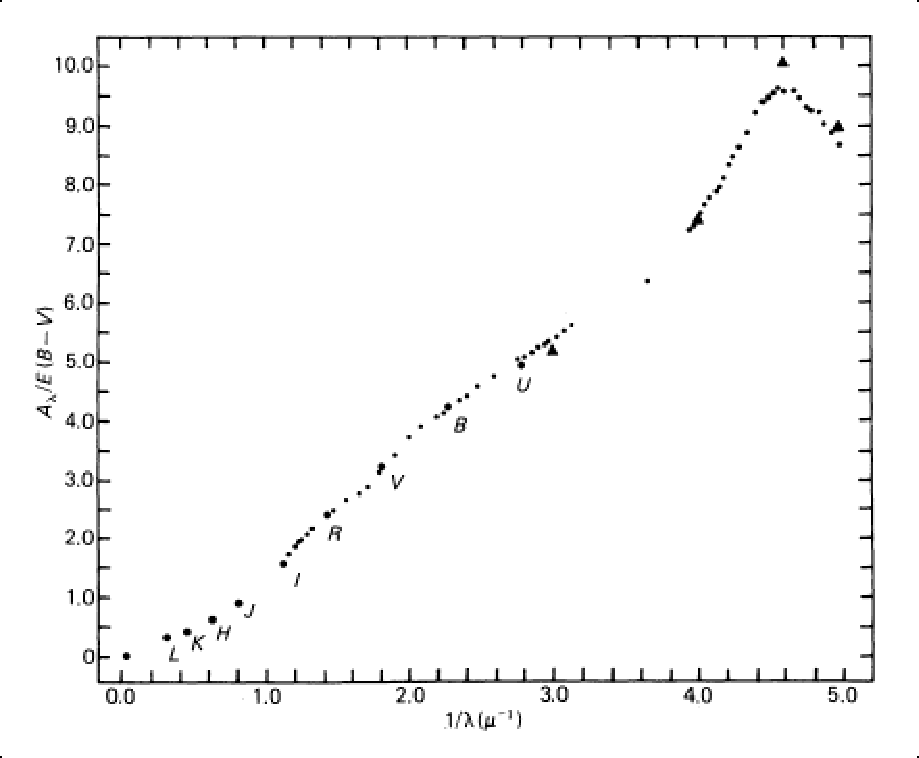
\includegraphics[width=0.5\textwidth]{interstellarreddeningreduite}
  \label{extinction}
  \caption{Variation de $A_V/E_{B-V}$ en fonction de $1/\lambda$}
\end{figure}

\begin{Answer}
  \begin{enumerate}
  \item Calcul de l'extinction
    $$
    E_{B-V} = (A_B- A_V) = (B-V )- (B-V)_0 = 2,25-(-0,25) = 2
    $$
    Le graphique donne $A_V = 3 E_{B-V}$, d'où:
    $$
    A_V =3 \times 2 = 6
    $$
  \item Le graphique donne $A_K = 0.5 \times E_{B-V}$, d'où:
    $$
    A_K = 0.5 \times 2 = 1
    $$
  \item L'extinction est beaucoup plus faible dans l'IR que dans le
    visible.
  \end{enumerate}
\end{Answer}

\section{Galaxies}

\subsection{Classification morphologique des galaxies}

\begin{Exercise}[Propriétés « physiques » de la classification]
  En vous servant du tableau sur les propriétés quantitatives de la
  séquence de Hubble, répondez aux questions suivantes :
  \begin{enumerate}
  \item Que peut-on dire sur la fraction de gaz dans les galaxies
    selon le type morphologique ?
  \item Que peut-on dire de la densité surfacique de masse, en
    supposant que toute la masse des galaxies est concentrée dans un
    disque mince ?
  \end{enumerate}
\end{Exercise}

\begin{Answer}
  \begin{enumerate}
  \item La fraction de masse de gaz est donnée par le rapport de la
    masse de gaz à la masse totale. Ce rapport augmente des S0 aux
    irrégulières.
  \item La densité surfacique de masse est $S = M/ \pi R^2$. Elle
    diminue des S0 aux irrégulières.
  \end{enumerate}

  Dans le tableau ci-dessous, les valeurs de
  $M_{\mathrm{gaz}}/M_{\mathrm{totale}}$ et de $S$ sont obtenues
  statistiquement sur un échantillon de plusieurs milliers de
  galaxies. Ce ne sont donc pas les valeurs obtenues par le calcul
  direct sur les médianes, mais le comportement reste le même.

  \begin{center}
    \begin{tabular}{|c|c|c|c|c|c|c|}
      \hline
      Propriétés & E,SO & S0a,Sa & Sab,Sb & Sbc,Sc & Scd,Sd & Sm,Im \\
      \hline
      $M_{\mathrm{totale}}$ ($10^{10}M_{\odot}$) & & 22.6 & 32.4 & 19.0 & 7.9 &
      1.6 \\
      \hline
      $M_{\mathrm{gaz}}$ ($H$ neutre en $10^{9}M_{\odot}$) & 1.24 & 5.62 &
      15.14 & 15.85 & 9.33 & 2.40\\
      \hline
      $M_{\mathrm{gaz}}/M_{\mathrm{totale}}$ & & 0.03 & 0.05 & 0.08 & 0.11 & 0.15 \\
      \hline
      diamètre (kpc) & 21.1 & 19.8 & 25.1 & 22.4 & 17.7 & 8.5  \\
      \hline
      S ($M_{\odot}/pc^2$) &  & 188.9 & 154.7 & 124.2 & 91.4 & 74.5 \\
      \hline
    \end{tabular}
  \end{center}
\end{Answer}


\begin{Exercise}[de Vaucouleurs et autres classifications]
  Donnez la classification simplifiée (E, S0, SA, SAB, SB) des
  galaxies données dans la partie cours correspondante dans spirale.

  Est-il toujours facile de classifier les galaxies réelles?
\end{Exercise}

\begin{Answer}
  \begin{center}
    \begin{tabular}{|c|c|c|c|}
      \hline
      % \textbf{N° objet} & \textbf{Nom} & \textbf{Réponse} &
      % textbf{Classification complète dite RC3}\\ \hline
      1  & NGC6070    & SA  & SA(s)cd  \\ \hline
      2  & NGC 7424   & SAB & SAB(rs)cd  \\ \hline
      3  & MESSIER 31 & SA  & SA(s)b  \\ \hline
      4  & MESSIER 33 & SA  & SA(s)cd  \\ \hline
      5  & MESSIER 87 & E0 ou E1 & E+0-1 pec* \\ \hline
      6  & NGC 2683   & SA  & SA(rs)b  \\ \hline
      7  & NGC 1300   & SB  & (R')SN(r'1)b  \\ \hline
      8  & NGC 1097   & SB  & (R'\_1:)SB(r'l)b  \\ \hline
      9  & NGC 4321   & SAB & SAB(s)bc \\ \hline
      10 & MESSIER 83 & SAB & SAB(s)c \\ \hline
    \end{tabular}
  \end{center}

  Galaxies lointaines sans noms (11). La classification demandée est
  SB. Ces objets sont considérés comme des galaxies barrées mais n'ont
  pas été précisément classifiées à cause du manque de résolution des
  images (HST Deep Field North).

  *pec: 'peculiar' à cause du jet provenant du noyau actif
\end{Answer}

\subsection{Constituants des galaxies}

\begin{Exercise}[Les étoiles]
  Si l'on considère une sphère de rayon 10 kpc peuplée par $10^{11}$
  étoiles dont le rayon est égal à celui du soleil, calculez la
  fraction de volume occupé par les étoiles.
\end{Exercise}

\begin{Answer}
  La fraction est de $10^{11}\times \left(\frac{0.7\times
      10^{6}}{10\times 3.08\times 10^{16}}\right)^{3}\approx 10^{-20}$
\end{Answer}


\begin{Exercise}[La matière noire]
  Donnez l'expression de l'accélération $a$ centrifuge en fonction de
  $V$, et $R$, la vitesse circulaire d'une étoile à une distance $R$
  du centre de la galaxie.  Écrire la loi de Newton pour cette
  étoile~: l'accélération $a$ en fonction de la masse $M$ incluse dans
  le rayon $R$.  En déduire la loi de décroissance de $V$ en fonction
  du rayon $R$ de l'étoile, en supposant que la masse $M$ reste
  constante (c'est-à-dire que toute la masse de la galaxie est
  comprise dans la sphère de rayon $R$).
\end{Exercise}

\begin{Answer}
  L'accélération centrifuge est donnée simplement par $a = V^2/R$.  La
  loi de Newton nous dit alors que l'accélération de l'étoile est
  proportionnelle à la masse $M$ avec $a = G M/R^2$, où $G$ est la
  constante universelle de la gravitation.  On en déduit alors
  facilement que $V^2/R = GM/R^2$ donc $V^2 \propto M/R$.

  Si $M$ reste constant avec $R$ qui croit, alors $V^2$ doit décroître
  comme $1/R$.
\end{Answer}

\subsection{Exemple de galaxie : la Voie Lactée }

\begin{Exercise}[Morphologie de notre galaxie]
  En examinant en détail l'image de notre galaxie prise par COBE/DIRBE
  (Fig.~\ref{cobe}) on distingue que le bulbe de la Voie Lactée n'est
  pas symétrique.
  \begin{enumerate}
  \item Examiner cette image et essayer de mesurer la hauteur du
    bulbe~; à droite, puis à gauche du centre de la Galaxie
  \item Donner une explication plausible de cette asymétrie, en se
    rappelant notre position très particulière par rapport au centre
    de notre galaxie, et en se rappelant des différentes composantes
    qui composent notre Galaxie.
  \end{enumerate}
\end{Exercise}

\begin{figure}[htp]
  \centering
  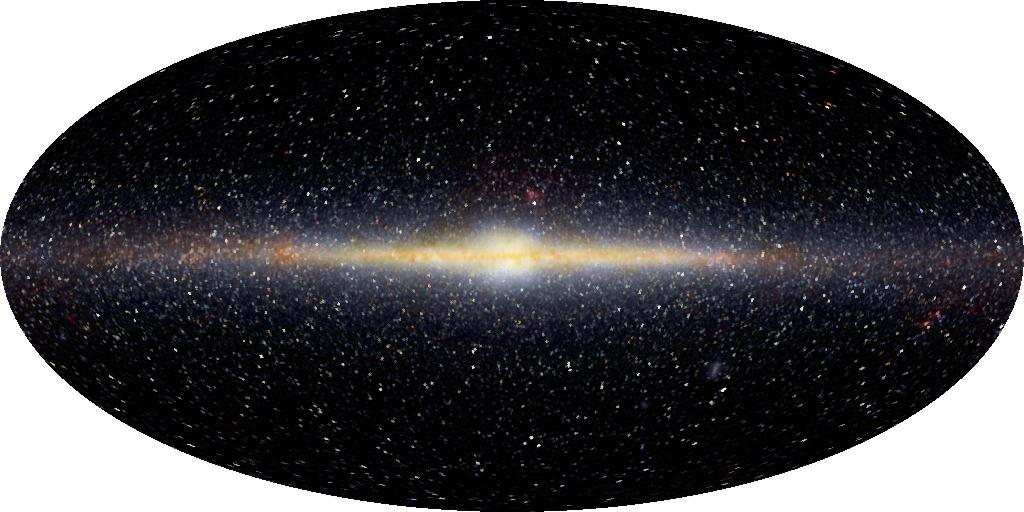
\includegraphics[width=0.8\textwidth]{milky2w}
  \label{cobe}
  \caption{Notre galaxie vue par COBE/DIRBE.}
\end{figure}

\begin{Answer}
  Le bulbe de la galaxie vue en infrarouge est effectivement
  asymétrique:
  \begin{enumerate}
  \item Le coté gauche a une épaisseur légèrement plus grande que le
    coté droit.
  \item Ça n'est pas un effet de populations stellaires, ou
    d'extinction due à la poussière, mais bien une épaisseur
    réellement plus grande d'un coté que de l'autre. Ce que l'on voit
    est en fait un effet de projection : c'est en fait la barre de la
    Galaxie que nous observons. Cette barre étant inclinée à 35 degrés
    environ par rapport à nous, le coté gauche étant proche de nous,
    le coté droit loin de nous (de l'autre coté du centre
    galactique). Une des extrémités de la barre est donc plus proche
    de nous, et par projection elle apparaît plus haute...
  \end{enumerate}
\end{Answer}

\begin{Exercise}[Le centre galactique]
  L'image ci-dessous (Fig.~\ref{centregalac}) montre l'orbite de
  l'étoile ayant la plus grande vitesse autour du centre galactique. À
  partir des données (période en années de 15.2 ans, et demi grand-axe
  de 0.119 arcsecondes) de cette orbite, retrouver l'estimation de la
  masse incluse dans ce rayon au centre de notre Galaxie en utilisant
  la troisième loi de Kepler. On rappelle que nous sommes à environ
  8.5~kpc du centre galactique et que G, la constante
  gravitationnelle, vaut $6,6742.10^{-11} m^3 kg^{-1} sec^{-2}$.  La
  masse visible étant estimée à environ 106 masses solaires, en
  déduire une estimation de la masse noire centrale (le fameux trou
  noir) de notre Galaxie.
\end{Exercise}

\begin{figure}[htp]
  \centering
  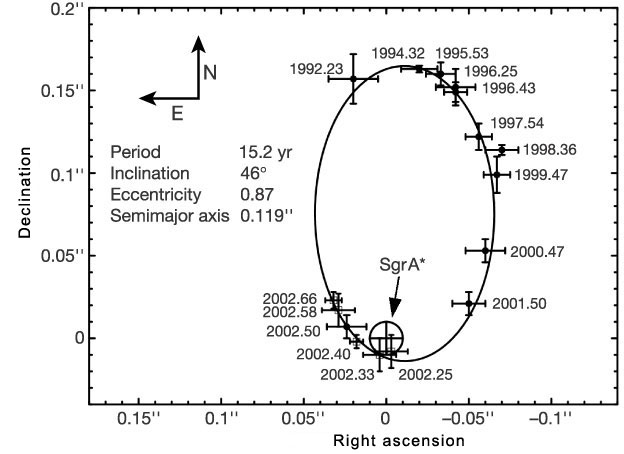
\includegraphics[width=0.5\textwidth]{nature01121-f2_2}
  \label{centregalac}
  \caption{Orbite de l'étoile S2 autour du centre galactique SgrA*
    (Schödel et al. 2002).}
\end{figure}

\begin{Answer}
  On rappelle que G, la constante gravitationnelle, vaut
  $6,6742.10^{-11} m^3kg^{-1}sec^{-2}$

  Nous allons d'abord transformer la taille du demi grand-axe
  d'arcseconde en mètres, et ensuite, la période en secondes:
  \begin{itemize}
  \item 1 arcseconde équivaut à $1/3600$~degrés, donc à $8.5~kpc$ ,
    cela revient à environ $0.041~pc$. Le demi grand axe est donné
    comme étant égal à $0.119$~arcseconde, donc cela équivaut à~:
    $$
    a = 0.119\times0.041 = 0.0048~pc = 0.0048\times 3.08 \times
    10^{16} = 1.5 \times 10^{14}~m
    $$

  \item la période $T$ est donnée de 15.2 ans donc~: $T=479347200~s$
  \end{itemize}

  Enfin la troisième loi de Kepler dit que le rapport $T^2/a^3$ est une
  constante k qui ne dépend que de la masse du système.

  Cette constante k est simplement donnée par : $4\pi^2/(GM)$ donc on
  peut écrire que:
  $$
  M = \frac{4\pi^2 a^3}{T^2 G}
  $$

  En application numérique cela donne (en kg, vérifiez bien que
  l'équation est homogène dans ses unités):
  $$
  M = \frac{ 4 \times \pi^2 \times (1,5 \times 10^{14})^3 } { (479 347
    200)^2 \times 6,6742 \times 10^{11} } = 8,7 \times 10^{36}~kg
  $$
  et ceci exprimé en masses solaires: $M \approx 4,4 \times
  10^6~M_{\odot}$
\end{Answer}

\subsection{Le groupe local}

\begin{Exercise}
  Compter le nombre de galaxies ayant un diamètre plus petit que 6
  kpc, et celles ayant un diamètre plus grand. Quelles sont les
  galaxies qui dominent en nombre ? Et en luminosité totale ?
  (Fig.~\ref{listgalac})
\end{Exercise}

\begin{figure}[htp]
  \centering
  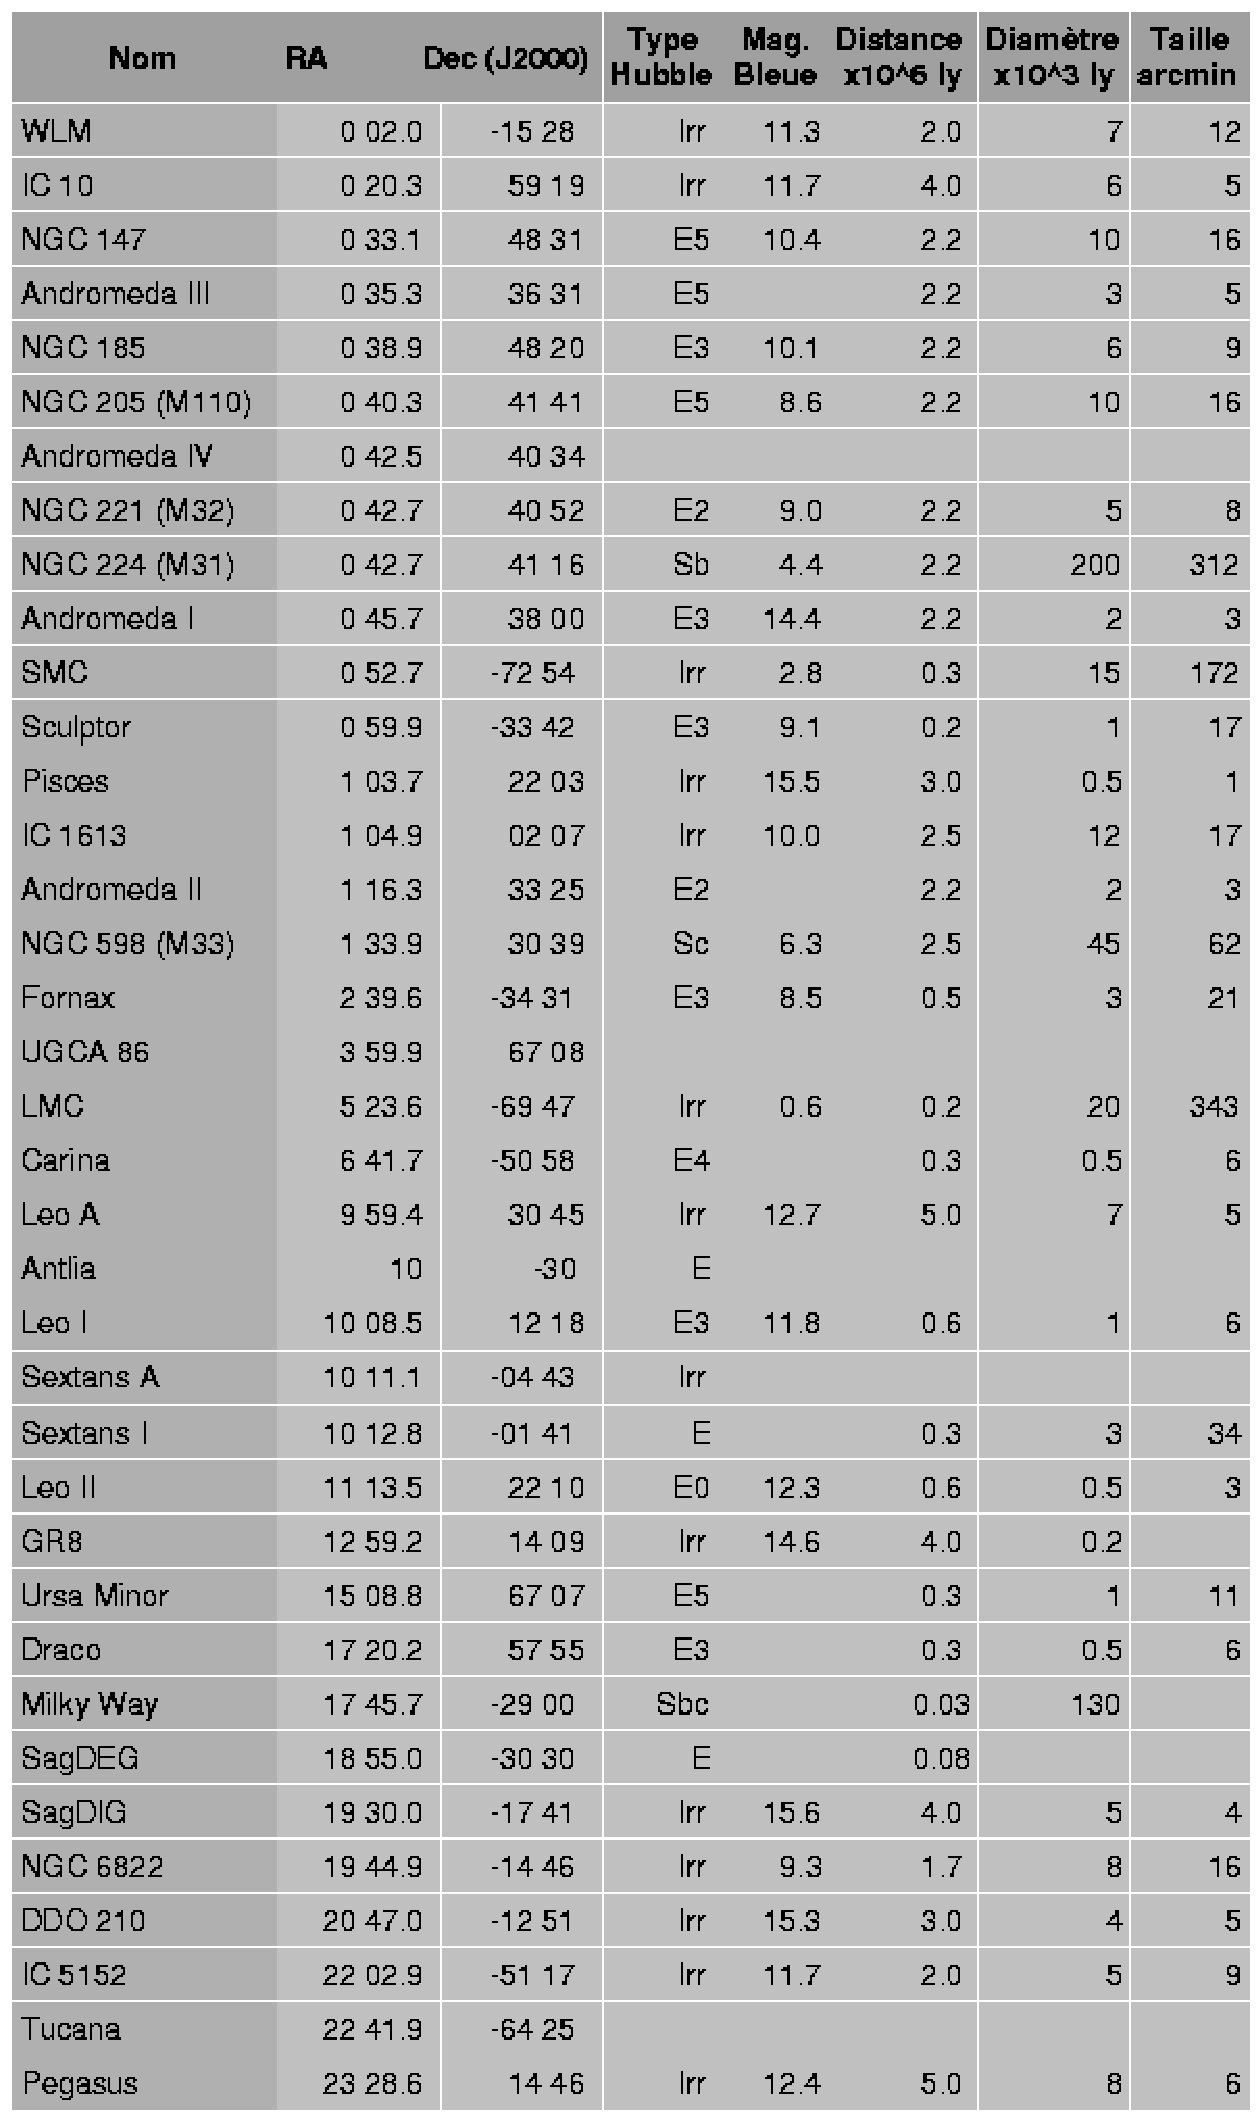
\includegraphics[height=\textheight]{listegalaxiegroupelocal}
  \label{listgalac}
  \caption{Liste des galaxies du Groupe Local, avec leurs noms, leurs
    positions sur le ciel, le type de Hubble, la distance, le diamètre
    en milliers d'années-lumière et en arcminutes sur le ciel.}
\end{figure}

\begin{Answer}
  Il y a 26 petites galaxies -- dites « naines » -- sur les 30
  galaxies dont on nous donne la taille, et seulement 2 galaxies avec
  un diamètre de plus de 30 kpc : M31 et la Voie Lactée). Ce sont donc
  les galaxies naines qui dominent en nombre, mais elles ne dominent
  pas en luminosité totale.
\end{Answer}

\subsection{Distribution des galaxies dans l'univers}

\begin{Exercise}[Fonction de luminosité]
  \begin{enumerate}
  \item Exprimer la loi de Schechter en magnitudes absolues.
  \item Quelle est la signification physique de la loi de Schechter?
  \end{enumerate}
\end{Exercise}

\begin{Answer}
  \begin{enumerate}
  \item En magnitude
    $$
    \Phi (M) = 0.4 \ln (10) \Phi ^{*}10^{0.4(\alpha +1)(M^{*}-M)}\exp
    \left( -10^{0.4(M^{*}-M)} \right)
    $$

  \item Cette fonction empirique montre bien la prédominance des
    galaxies de faible luminosité intrinsèque.
  \end{enumerate}
\end{Answer}

\subsubsection{Effets d'environnement, collisions et fusions}

\begin{Exercise}[Calcul de la fréquence des collisions dans un
  amas]
  On considère un amas de galaxies qui a les caractéristiques
  suivantes:
  \begin{itemize}
  \item il est supposé sphérique, de diamètre $D_{amas}$ en pc
  \item il contient $N_{galaxies}$ identiques et réparties
    uniformément dans l'amas
  \item les galaxies sont supposées animées d'une vitesse uniforme
    $v_{galaxies}$ en km/s
  \end{itemize}

  \begin{enumerate}
  \item Donner l'expression de la densité numérique de galaxies dans
    l'amas en $pc^{-3}$.

  \item On suppose maintenant que les galaxies ont un diamètre typique
    $D_{galaxies}$ (en pc). En modélisant les galaxies comme des
    sphères dures (boules de billard...) de diamètre $D_{galaxies}$,
    donner l'expression de la section efficace $S_{efficace}$ (en
    $pc^2$) lors d'une collision/interaction entre deux galaxies.

  \item Donner l'expression du nombre de collisions/interactions que
    subit une galaxie de l'amas pendant la durée $dt$ (en années). En
    déduire, pour une galaxie, le temps caractéristique de collision
    et le libre parcours moyen.

  \item En déduire le temps entre deux collisions/interactions dans
    l'amas.

  \item Calcul de la fréquence des collisions dans un amas:
    Considérons un amas de $N=850$ galaxies dont le diamètre est
    $D=7~Mpc$ et dont la dispersion des vitesses est $V =
    650~km/s$. Explicitez le calcul numérique du temps moyen entre
    deux collisions pour l'amas considéré.
  \end{enumerate}
\end{Exercise}

\begin{Answer}
  \begin{enumerate}
  \item Le volume de l'amas est
    $$
    V_{amas}=\frac{\pi}{6}D_{amas}^3
    $$
    et la densité numérique de galaxies est donc
    $$
    n_{galaxies}=\frac{N_{galaxies}}{V_{amas}}=
    \frac{6N_{galaxies}}{\pi D_{amas}^3}
    $$
    (en nombre de galaxies par $pc^3$ si le diamètre de l'amas est en
    pc)

  \item Deux galaxies entreront en collision/interaction lorsqu'elle
    passent à une distance < $D_{galaxies}$ l'une de l'autre. La
    section efficace de collision est donc $S_{efficace}=\pi
    D^2_{galaxies}$ en $pc^2$ si le diamètre des galaxies est exprimé
    en $pc$.

  \item Le volume «balayé» par une galaxie pendant le temps dt est le
    suivant:
    $$
    V = \frac{3.15\,10^7 \text{(s par année)}}{%
      3.09\,10^{13} \text{(km par pc)}}
    \times v_{galaxies} \times S_{efficace} \times dt
    $$
    Le nombre de collisions pendant ce temps $dt$ est donc
    $N_{collision} = n_{galaxie}V$. Le temps caractéristique de
    collision/interaction $t_{collision}$ correspond à $dt$ tel que
    $N_{collisions} = 1$. Le libre parcours moyen est $l =
    v_{galaxies} \times t_{collision}$.
    $$
    \tau_{collision} =
    \frac{3.09 \times 10^{13}}{6 \times 3.15 \times 10^7}
    \frac{D^3_{amas}}{D^2_{galaxies} \times v_{galaxies} \times N_{galaxies}}
    $$

  \item Le temps caractéristique de collision/interaction dans l'amas
    est $t_{collision}^{amas} = \tau_{collision}/N_{galaxies}$ (on
    considère ici l'amas entier et non plus une galaxie unique).
  \end{enumerate}

\end{Answer}



\subsection{Équilibre gravitationnel}

\begin{Exercise}[Théorème du Viriel scalaire]
  Le théorème du Viriel peut aussi s'écrire :
  $$
  \frac{2K}{U}=-1
  $$
  Imaginez que vous vouliez construire un système stellaire, en
  donnant à $N$ étoiles leurs positions et leurs vitesses, et où vous
  auriez:
  $$
  \frac{2K}{U}>-1
  $$
  \begin{enumerate}
  \item Comment feriez-vous ? (donner un exemple)
  \item Comment le système évoluerait-il ?
  \end{enumerate}
\end{Exercise}

\begin{Answer}
  \begin{enumerate}
  \item Il suffit de donner une position quelconque aux étoiles mais
    en leur donnant à toute une vitesse nulle. On aurait alors $K=0$,
    et ainsi on aurait bien la condition remplie!

  \item Si cette condition est remplie, c'est que l'énergie cinétique
    est trop faible par rapport à l'énergie potentielle (en valeur
    absolue). Il manque aux étoiles de la vitesse pour que le système
    reste à l'équilibre, et il va donc se réarranger, avec un rayon
    plus petit.
  \end{enumerate}
\end{Answer}

\begin{Exercise}[Application du théorème du Viriel]
  On va maintenant utiliser le théorème du Viriel pour remplir le
  tableau ci-dessous, donnant les rayons, masses et vitesse
  caractéristiques de différents système stellaires.  Veuillez
  compléter ce tableau.  (On prendra $G$ en fonction d'unités
  astronomiques pratiques, ainsi $G=0.004301$
  pc.km$^{2}$.s$^{-2}$.M$_{\odot}^{-1}$)

  \begin{center}
    \begin{tabular}{|c|c|c|c|}
      \hline
      Système & R (pc) & V (km/s) & M ($M_{\odot}$) \\ \hline
      Amas globulaire & 10 & 10 &  \\ \hline
      Galaxie & 50~000 & 200 & \\ \hline
      Amas de galaxies & 1~000~000  & 1000  &  \\ \hline
    \end{tabular}
  \end{center}
\end{Exercise}

\begin{Answer}
  \begin{center}
    \begin{tabular}{|c|c|c|c|}
      \hline
      Système & R (pc) & V (km/s) & M ($M_{\odot}$) \\ \hline
      Amas globulaire & 10 & 10 & $1,4\times 10^6$ \\ \hline
      Galaxie & 50~000 & 200 & $2,3\times 10^{11}$ \\ \hline
      Amas de galaxies & 1~000~000  & 1000  &  $1,4\times 10^{15}$ \\ \hline
    \end{tabular}
  \end{center}
\end{Answer}

\begin{Exercise}[Temps cinématique]
  On va maintenant calculer le temps cinématique $t_c$ pour différents
  systèmes stellaires. Veuillez compléter le tableau ci-dessous.  (Une
  fois de plus, on prendra $G$ en fonction d'unités astronomiques
  pratiques, ainsi $G=0.004301$ pc.km$^{2}$.s$^{-2}$.M$_{\odot}^{-1}$)
  \begin{center}
    \begin{tabular}{|c|c|c|c|}
      \hline
      Système & R (pc) & M ($M_{\odot}$) & $t_c$ (ans) \\ \hline
      Amas ouvert & 1 & 500 &  \\ \hline
      Amas globulaire & 10 & $10^5$ &  \\ \hline
      Galaxie & 50~000 & $10^{12}$ & \\ \hline
    \end{tabular}
  \end{center}
  Que remarquez-vous sur ces temps cinématiques pour les différents
  systèmes ?
\end{Exercise}

\begin{Answer}
  \begin{center}
    \begin{tabular}{|c|c|c|c|}
      \hline
      Système & R (pc) & M ($M_{\odot}$) & $t_c$ (ans) \\ \hline
      Amas ouvert & 1 & 500 & $10^6$ \\ \hline
      Amas globulaire & 10 & $10^5$ & $2\times 10^6$ \\ \hline
      Galaxie & 50~000 & $10^{12}$ & $2\times 10^8$ \\ \hline
    \end{tabular}
  \end{center}

  Les temps cinématiques pour un amas ouvert et un amas globulaire ne
  sont pas vraiment différents malgré leurs tailles respectives très
  différentes.  De même entre une galaxie et un amas globulaire: il ne
  faut qu'environ 100 plus de temps à une étoile avec une vitesse
  typique pour traverser une grosse galaxies qu'un amas globulaire
  (bien sur les vitesses caractéristiques ne sont pas les mêmes pour
  ces 2 systèmes).
\end{Answer}

% ===============================================================================

\chapter{Vie des structures - Cosmologies}

\section{Espace et temps absolus}

\begin{Exercise}[La faiblesse de la force de gravitation]
  Marcel et Naomi ressentent l'un pour l'autre une certaine attirance;
  quelle part en revient tout bêtement à la force de gravitation
  universelle, lorsque leurs centres de gravité respectifs sont
  distants de 1 mètre ?  Quelle masse, au même point de la Terre,
  présente un poids égal à cette force ?  Marcel pèse, à Lyon, 700 N,
  et Naomi 580 N.  Le rayon de la Terre à Lyon sera supposé égal à
  6365~km.  La constante de la gravitation et la masse de la Terre
  sont données dans les annexes du cours...
\end{Exercise}

\begin{Answer}
  Il s'agit, simplement, d'appliquer la formule de Newton deux fois
  pour trouver les masses respectives de Marcel et Naomi, puis une
  troisième fois pour calculer l'attraction qui s'exerce entre eux, en
  prenant garde aux unités.
  $$
  F = G \frac{m_1 m_2}{d^2}
  $$

  On retrouve d'abord les valeurs des constantes : $G = 6,672 \times
  10^{-11}$, $M_{\oplus} = 5,976 \times 10^{24}~kg$, et $R = 6365~km$
  qui est donné dans l'énoncé.

  On écrit donc:
  $$
  P_{\mathrm{Marcel}} = G \frac{M_{\mathrm{Marcel}}M_{\oplus}}{R^2}
  $$
  soit encore:
  $$
  M_{\mathrm{Marcel}} = \frac{P_{\mathrm{Marcel}}R^2}{G M_{\oplus}}
  $$
  et donc
  $$
  M_{\mathrm{Marcel}} = \frac{ 6370000^2 \times 700 }{ 6,672 \times
    10^{-11} \times 5,976 \times 10^{24} } = 71,23~kg
  $$
  Cette valeur s'obtiendrait aussi en utilisant la formule $P =
  M_{\mathrm{Marcel}}\times g$, où $g$ est l'accélération de la
  pesanteur à Lyon. Mais l'énoncé ne précise pas la valeur de $g$ à
  Lyon...

  Pour Naomi, on peut utiliser le fait que
  $M_{\mathrm{Naomi}}/M_{\mathrm{Marcel}} =
  P_{\mathrm{Naomi}}/P_{\mathrm{Marcel}}$, puisque les deux personnes
  sont soumises au même champ de gravité. Et donc:
  $$
  M_{\mathrm{Naomi}} = M_{\mathrm{Marcel}}
  \frac{P_{\mathrm{Naomi}}}{P_{\mathrm{Marcel}}} = 71,23 \times
  \frac{58}{70} = 59,02~kg
  $$
  D'où $F_{\mathrm{Naomi}-\mathrm{Marcel}} = ( 6,672 10^{-11} \times
  71,23 \times 59,02 ) / 1 = 2,8 10^{-7}~N$.

  La masse qui présenterait un poids égal à cette valeur en cet
  endroit serait de : $M = ( 63700002 \times 2,8 10^{-7} ) / ( 6,672
  10^{-11} \times 5,976 10^{24} ) = 2,85 10^{-8} kg = 28,5~\mu g$.

  Elle peut également se calculer, d'après une remarque déjà faite,
  par $M = 71,23 \times 2,8 10^{-7} / 700$. L'attraction
  gravitationnelle est une force \emph{très faible}, c'est même la
  plus faible des quatre forces fondamentales de l'univers...
\end{Answer}

\subsection{Problèmes de l'univers de Newton}

\begin{Exercise}[L'instabilité gravitationnelle]
  Pourquoi Newton pense-t-il que ces trois hypothèses supplémentaires
  permettraient, chacune, de « sauver » l'univers de la catastrophe
  gravitationnelle?
\end{Exercise}

\begin{Answer}
  \begin{itemize}
  \item Si l'univers est infini, tout point est entouré d'une
    distribution de matière à symétrie sphérique, et restera donc
    immobile.
  \item Si l'univers est en expansion, et bien, tant qu'il l'est,
    c'est qu'il n'est pas en train de se contracter !
  \item Si l'univers est très jeune, il n'a pas encore eu le temps de
    démarrer sa contraction gravitationnelle de façon sensible, et
    voilà ...
  \end{itemize}
\end{Answer}

\begin{Exercise}[Le paradoxe d'Olbers]
  En quoi le fait que l'univers soit jeune et en expansion peut-il
  permettre d'expliquer la noirceur du ciel nocturne ?
\end{Exercise}

\begin{Answer}
  \begin{itemize}
  \item Si l'univers est jeune, du fait de la vitesse finie de
    propagation de la lumière, celle qui provient des objets très
    lointains n'a pas eu le temps de nous parvenir.
  \item Si l'univers est en expansion, la lumière qui nous parvient
    des objets très lointains a été affaiblie par cette expansion
    (ceci sera traité plus loin dans le cours), au point de ne pas
    être détectable.
  \end{itemize}
\end{Answer}

\section{La rupture relativiste}

\subsection{Vitesse de la lumière}

\begin{Exercise}[La première mesure de $c$]
  Si Roemer a fait le calcul (ce que l'on ignore, mais cela semble
  assez probable), et en supposant qu'il utilisait la même valeur de
  la distance Terre-Soleil que les astronomes d'aujourd'hui, quelle
  valeur de $c$ a-t-il obtenue?
\end{Exercise}

\begin{Answer}
  Si la lumière met $8+8 = 16$ minutes pour traverser l'orbite de la
  Terre, c'est à dire pour franchir une distance de $2~U.A$., sa
  vitesse est $c = 2 \times 1,49598 \times 10^{11} / ( 16 \times 60 )
  = 3,11 \times 10^8~m~s^{-1}$. Ceci suppose que la valeur de
  l'U.A. admise alors était la même qu'aujourd'hui, ce qui n'est
  certainement pas exact : en 1675, on n'avait pas encore très bien
  mesuré la distance de la Terre au Soleil ... La valeur de deux fois
  huit minutes est elle-même approximative. Roemer aurait plutôt
  trouvé $2 \times 10^8~m~s-1$, dit-on. La première détermination
  sérieuse de l'Unité Astronomique est due à Cassini et Richer, en
  1671. Il faudra attendre le XXe siècle et les méthodes d'écho radar
  pour disposer de mesures très précises de cette valeur.
\end{Answer}

\subsection{Relativité générale}

\subsubsection{Einstein dans l'ascenseur}

\begin{Exercise}[L'équivalence gravité/accélération]
  On dit que, pour la Relativité Générale, gravitation et accélération
  sont équivalentes, mais que cette équivalence n'est que
  locale. C'est à dire qu'aucune expérience de physique ne permet de
  distinguer les effets de l'une de ceux de l'autre, mais seulement
  tant qu'on se limite à un très petit domaine spatial. En gros, c'est
  à peu près vrai dans un dé à coudre, cela ne l'est plus vraiment
  dans un stade de foot...

  En reprenant l'exemple simple de l'ascenseur d'Einstein, pouvez-vous
  montrer qu'en effet il est facile de distinguer pesanteur et
  accélération par la fusée si on abandonne la localité. Il suffit de
  modifier l'ascenseur...
\end{Exercise}

\begin{Answer}
  À grande échelle, le champ de gravité qui environne un corps massif
  reste en général tout à fait discernable d'une accélération
  constante.  Par exemple, dans l'image de l'ascenseur utilisée dans
  le cours, il ne faut pas que la cabine soit trop étendue. Sinon, le
  parallélisme ou le non-parallélisme des actions sur des masses très
  éloignées l'une de l'autre trahirait la « vraie » nature du champ.
  La cabine de gauche, supposée à grande distance de la planète, et
  accélérée vers le haut (flèche bleue), produit des actions
  parallèles (flèches rouges) sur les deux masses-test. La cabine de
  droite, immobile dans le champ de gravitation de la Terre, montre
  des actions convergentes vers le centre de la Terre (flèches
  vertes). Rusés comme ils le sont parfois, les physiciens de
  l'ascenseur finiraient par s'en apercevoir... (Fig.~\ref{grav})

  \begin{figure}[htp]
    \centering
    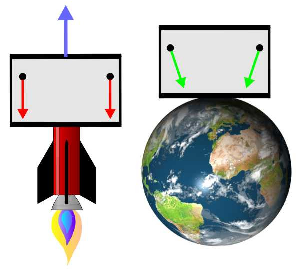
\includegraphics[width=0.4\textwidth]{grav}
    \caption{}
    \label{grav}
  \end{figure}
\end{Answer}

\subsection{Les tests}

\begin{Exercise}[Le décalage gravitationnel vers le rouge]
  Une lampe spectrale émettant la raie Hydrogène Alpha (de longueur
  d'onde en laboratoire 656,3 nm) est utilisée pour communiquer à
  partir d'une capsule en orbite serrée autour d'une étoile à
  neutrons. Le rayon de l'orbite est de 1000 km, la masse de l'étoile
  de 1,5 masses solaires.  À quelle longueur d'onde le vaisseau qui a
  lancé la capsule, et se tient prudemment à grande distance, doit-il
  rechercher les signaux?
\end{Exercise}

\begin{Answer}
  Le décalage gravitationnel subi à la distance r d'un corps de masse
  M s'écrit:
  $$
  z = \frac{GM}{c^2r}
  $$
  Et donc:
  $$
  z = \frac{ 6,672 \times 10^{-11} \times 1,5 \times 1,989 \times
    10^{30} }{ 2997924582 \times 10^6 } = 2,215 \times 10^{-3}
  $$
  Mais:
  $$
  z = \frac{ \delta \lambda } { \lambda_0 }
  $$
  Et donc:
  $$
  \lambda = \lambda_0 + \delta \lambda = (1+z)\lambda_0
  $$
  D'où le $\lambda$ cherché: $\lambda = 1,00221 \times 656,3 =
  657,75~nm$.
\end{Answer}

\section{Le big bang}

\subsection{Expansion de l'univers...}

\begin{Exercise}[...limitée par $c$?]
  Plus une galaxie est éloignée de notre Voie Lactée, plus les
  astronomes lui trouvent une vitesse d'éloignement élevée. C'est
  l'expansion de l'univers. Mais, quand la distance croît sans cesse,
  elle atteint un moment une valeur $d_c$ telle que :
  $$
  V = H_0 d_c > c
  $$
  Invraisemblable, n'est-ce pas ?
\end{Exercise}

\begin{Answer}
  Il est interdit par la Relativité Générale de mesurer une vitesse
  égale ou supérieure à $c$ pour un objet de masse non nulle, comme
  une galaxie. Alors ?

  Alors, cela ne pose aucun problème pour l'expansion de l'univers, où
  les objets (les galaxies...) sont immobiles dans un espace dont la
  géométrie s'étire. Les galaxies très lointaines voient effectivement
  leur vitesse apparente atteindre celle de la lumière, et
  disparaissent alors de l'univers observable. Ceci n'enlève rien au
  fait qu'elles continuent à s'éloigner de nous à des vitesses
  supérieures à $c$.

  Signalons que nos moyens d'observation actuels sont loin de nous
  permettre d'observer les objets qui flirtent avec cette limite...
\end{Answer}

\begin{Exercise}[...la même partout?]
  La radiogalaxie 3C 171 (nommée ainsi parce qu'elle occupe la 171e
  position dans le troisième catalogue de radiources établi par
  l'observatoire de Cambridge...) est relativement lointaine;
  entraînée par l'expansion de l'univers, elle présente une vitesse de
  fuite de 63000 km par seconde.

  Montrer que malgré cela, l'astronome Xhbrr'ffttk, qui a là-bas
  découvert l'expansion de l'univers, comme Hubble l'a fait pour nous,
  a lui aussi trouvé une loi qui s'écrit :
  $$
  V_0 = X_0 d_{0^{'}} \quad\text{avec}\quad X_0 = H_0
  $$
  $V_0$ étant la vitesse mesurée à partir de 3C171 pour une galaxie
  lointaine située à la distance $d_0$ de 3C171, et $X_0$ étant bien
  entendu la constante de Xhbrr'ffttk.

  Ainsi, d'une planète de 3C171, comme de la Terre, on observe la même
  expansion universelle, avec la même géométrie, et le même taux...
\end{Exercise}

\begin{Answer}
  Désignons par $V_T$ et $d_T$ les vitesses et distances mesurées à
  partir de la Terre, $V_{3C}$ et $d_{3C}$ celles mesurées à partir de
  3C171.  La vitesse de récession de 3C171 mesurée de la Terre est
  donc $v_T(3C171) = 63000~km/s$.

  Considérons une autre galaxie, G, observée à la fois de la Terre et
  de 3C171. On peut écrire :
  \begin{eqnarray*}
    \vec{V}_{3C}(G) &=& \vec{V}_{3G}(T) + \vec{V}_{T}(G) \\
    &=& -\vec{V}_{T}(3C171) + \vec{V}_{T}(G) \\
    &=& -H_0\vec{d}_{T}(3C171) + H_0\vec{d}_{T}(G) \\
    &=& H_0 \left[ \vec{d}_{T}(G) - \vec{d}_{T}(3C171) \right ] \\
    &=& H_0 \vec{d}_{3C}(G)
  \end{eqnarray*}
  et donc, à partir de 3C171 comme de la Terre, toute les galaxie
  observée semble s'enfuir avec une vitesse proportionnelle à sa
  distance, et le facteur de proportionnalité (la constante de
  Xhbrr'ffttk) est universel : $X_0=H_0$... (Fig.~\ref{H0})

  \begin{figure}[htp]
    \centering
    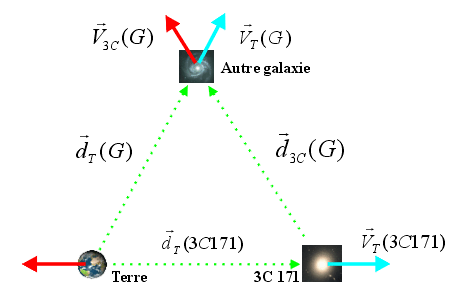
\includegraphics[width=0.4\textwidth]{351922_281}
    \caption{}
    \label{H0}
  \end{figure}
\end{Answer}

\begin{Exercise}[Le facteur d'expansion de l'espace]
  Donner $H_0$ en kilomètres par seconde et par mégaparsec est
  pratique pour les astronomes, mais ne parle guère à l'imagination.
  Passons donc dans des unités plus gouleyantes : si l'on suppose que
  $H_0 = 65 km s^{-1} Mpc^{-1}$, quelle est la valeur de
  l'accroissement annuel d'un kilomètre ? Des mètres ? Des millimètres
  ? Encore moins ?  Beaucoup plus?
\end{Exercise}

\begin{Answer}
  Un mégaparsec (Mpc) vaut $10^6$ parsecs, soit $3.26 10^6$
  années-lumière, soit $3,08 10^{19}~km$... Ceci nous montre que
  $65~km~s^{-1}~Mpc^{-1}$ équivalent à $2,10
  10^{18}~km~s^{-1}~km^{-1}$, ou encore $6,65
  10^{-11}~km~an^{-1}~km^{-1}$. Ce qui signifie que chaque kilomètre
  de l'espace, loin de toute galaxie, s'étire chaque année de $6,65
  10^{-11}~km$, soit environ 67 nanomètres! C'est infiniment dérisoire
  sur un kilomètre, mais sur les distances cosmiques l'effet est
  cumulatif, et cela donne des vitesses qui peuvent être très
  importantes, facilement de l'ordre de celle de la lumière...
\end{Answer}

\subsection{Facteur d'échelle}

\begin{Exercise}[Redshift et facteur d'échelle]
  La radiogalaxie 4C41.17 montre une raie spectrale intense à
  583,2~nm.  Cette raie est identifiée comme la raie Lyman alpha de
  l'hydrogène. En laboratoire, sur la Terre, la longueur d'onde de
  cette raie est de 121,5~nm. Quel était le facteur d'échelle de
  l'univers à l'époque où les atomes d'hydrogène de 4C41.17 émettaient
  cette raie ?
\end{Exercise}

\begin{Answer}
  Il suffit de se souvenir de la relation:
  $$
  1 + z = \frac{\lambda_\text{observé}}{\lambda_\text{émis}} =
  \frac{R_0}{R_\text{émission}}
  $$
  pour trouver $R_{em} = R_0 \times \lambda_{em}/\lambda_0 =
  \lambda_{em}/\lambda_{0}$. Et donc $R_{em} = 121,5/583,2 = 0,208$.
  À l'époque où 4C41.17 émettait la lumière qui nous parvient
  aujourd'hui, l'univers était cinq fois moins « étiré »
  qu'aujourd'hui... Remarquez bien qu'on évite de dire qu'il était
  moins « étendu » : cette expression sous-entendrait des choses sur
  la « taille globale » de l'univers, ce que tout cosmologiste
  raisonnable évite soigneusement de faire, vu son ignorance.
\end{Answer}

\begin{Exercise}[Facteur d'échelle et époque]
  À quelle époque $t_{em}$ la radiogalaxie 4C41.17 de l'exercice
  précédent a-t-elle émis la lumière que nous recevons aujourd'hui à
  $t_0$? On prendra $t_0 = 13.5$ milliards d'années.
\end{Exercise}

\begin{Answer}
  Il suffit de se souvenir de la relation liant le facteur d'échelle
  et le temps cosmologique :
  $$
  R(t)/R_{0} = \left(\frac{t}{t_0}\right)^{2/3}
  $$
  pour trouver $t_{em} = t_0 \times
  \left(R(t_{em})/R_{0}\right)^{3/2}$, et donc $t_{em} = 13,5 \times
  (0,208)^{1,5} = 1,3$~Gan.  4C41.17 émettait la lumière qui nous
  parvient aujourd'hui alors l'univers était âgé d'environ 1,3
  milliards d'années. Environ, car l'équation de départ n'est qu'une
  approximation.
\end{Answer}

\begin{Exercise}[Redshift cosmologique]
  Quel est le redshift de la radiogalaxie 4C41.17 citée dans
  l'exercice précédent?
\end{Exercise}

\begin{Answer}
  On reprend la relation:
  $$
  1 + z = \frac{\lambda_\text{observé}}{\lambda_\text{émis}} =
  \frac{R_0}{R_\text{émission}}
  $$
  pour trouver $1 + z = 1 / 0,208 = 4,807$, et donc $z = 3,807$.
\end{Answer}

\subsection{Film des débuts}

\begin{Exercise}[Nucléosynthèse primordiale ou non?]
  Les éléments légers $\mathrm{H}$, ${}^{2}\mathrm{H}$,
  ${}^{3}\mathrm{H}$, ${}^{4}\mathrm{He}$, ${}^{7}\mathrm{Li}$ sont
  nés avec le Big Bang. Mais d'où proviennent tous les autres éléments
  « lourds », ceux qui entrent dans la composition des objets du
  quotidien ?
\end{Exercise}

\begin{Answer}
  Les chapitres traitant des modèles stellaires et de l'évolution
  stellaire nous fournissent la réponse :
  \begin{itemize}
  \item Jusqu'au ${}^{56}\mathrm{Fe}$, les noyaux sont produits par
    les étoiles.  La source d'énergie de celles-ci est d'origine
    thermonucléaire, et elles sont des usines à fabriquer, par fusion,
    des noyaux lourds à partir de noyaux plus légers.
  \item Au-delà, seules les explosions de supernovae atteignent des
    températures suffisantes (plusieurs $10^9~K$) pour pouvoir
    synthétiser les noyaux très lourds, jusqu'aux éléments
    transuraniens.
  \item Quelques noyaux particuliers (${}^{6}\mathrm{Li}$,
    ${}^{9}\mathrm{Be}$, ${}^{10}\mathrm{B}$) sont sans doute formés
    lors des collisions des rayons cosmiques avec la matière
    interstellaire.
  \end{itemize}
\end{Answer}


\section{Questions diverses}

\subsection{Âge de l'univers}

\begin{Exercise}[Calcul du temps de Hubble]
  La valeur la plus probable, aujourd'hui, de la constante de Hubble
  est $H_0 = 65\;\u{km s^{-1} Mpc^{-1}}$ Quelle conclusion
  pouvez-vous en tirer sur l'âge réel de l'univers?
\end{Exercise}

\begin{Answer}
  Le temps de Hubble est défini par: $1/t_{H0} = H_0 =
  65~\u{km~s^{-1}~Mpc^{-1}}$. Il reste simplement à convertir les
  Mpc (megaparsecs) en kilomètres, et il vient : $1/t_{H0} =
  65~\u{km~s^{-1}} [3,26 10^{19}~\u{km}]^{-1} = 20 \times
  10^{-19}$~s, d'où $t = 5 \times 10^{17}~s = 16 \times
  10^9$~années. On peut donc penser que l'univers est âgé de moins de
  16~milliards d'années.
\end{Answer}

\begin{Exercise}[Age de l'univers et temps de Hubble]
  En partant de la définition de $H_0$ et de la relation trouvée dans
  la section précédente entre le facteur d'échelle $R$ et l'âge $t$ de
  l'univers dans le cas de la densité critique, trouver la relation
  entre $H$ et $t$.
\end{Exercise}

\begin{Answer}
  Par définition:
  $$
  v = H_0.d \quad\text{donc}\quad
  H_0 = \frac{v}{d} = \frac{\d d}{\d t} \frac{1}{d} =
  \frac{\d\left(\epsilon R \right)}{\d t}\frac{1}{\epsilon R}
  \hfill
  $$
  car toute distance, à un instant t, s'écrit:
  $$
  d = \epsilon R(t)
  $$
  où $\epsilon$ est une constante; Et donc:
  \begin{eqnarray*}
    H_0 &=& \frac{1}{R}\frac{\d R}{\d t} \\
    &=& \left ( \frac{t}{t_0} \right )^{-2/3} \times
    \frac{\d\left( \frac{t}{t_0} \right )^{2/3}}{\d t} \\
    &=& \left ( \frac{t}{t_0} \right )^{-2/3} \times
    \left( \frac{t}{t_0} \right)^{-1/3} \frac{2}{3} \frac{1}{t_0} \\
    &=& \left( \frac{t}{t_0} \right)^{-1} \times \frac{2}{3t_0} \\
    &=& \frac{2}{3t}
  \end{eqnarray*}
  Dans le cas critique (univers marginalement ouvert), l'âge de
  l'univers est égal aux deux-tiers du temps de Hubble.
\end{Answer}

\subsection{Distance de l'horizon}

\begin{Exercise}[{Temps de vol, distance, et expansion...}]
  Il y a dix milliards d'années, ce photon que nous recevons
  aujourd'hui a quitté une lointaine galaxie.
  \begin{enumerate}
  \item Cette galaxie se trouvait-elle à dix milliards
    d'années-lumière de nous au moment de l'émission ?
  \item Cette galaxie se trouve-t-elle aujourd'hui à dix milliards
    d'années-lumière de nous ?
  \end{enumerate}
\end{Exercise}

\begin{Answer}
  \begin{itemize}
  \item Le photon a voyagé pendant dix milliards d'années en luttant
    contre l'expansion de l'espace qui contrariait son mouvement; tout
    se passe comme s'il avait parcouru à la vitesse $c$ une distance
    supérieure à celle qui séparait la galaxie de nous au moment de
    l'émission.  Au moment de l'émission, la galaxie était donc à
    moins de dix milliards d'années-lumière de nous.
  \item Depuis que le photon a quitté la galaxie, celle-ci, entraînée
    par l'expansion, a continué à s'éloigner de nous. Le photon a bien
    parcouru (de son point de vue, en admettant qu'il en ait un) dix
    milliards d'années-lumière, puisque sa vitesse par rapport à
    l'espace est à tout instant égale à $c$, mais la galaxie a
    continué sa route pendant tout ce temps, et se trouve aujourd'hui
    à plus de dix milliards d'années-lumière de nous...
  \end{itemize}
\end{Answer}


% ==============================================================================

\chapter{Retour sur Terre - Nos repères dans le ciel}

\section{Se positionner dans le ciel}

\begin{Exercise}[Repérage]
  \begin{enumerate}
  \item Quelles sont les coordonnées horizontales des quatre points
    cardinaux?

  \item Peut-on définir les coordonnées horizontales pour un
    observateur installé au pôle Nord géographique ou au pôle Sud?

  \item Pour quelles valeurs de la hauteur et de la distance zénithale
    un astre est-il visible, c'est-à-dire au dessus de l'horizon?
  \end{enumerate}
\end{Exercise}

\begin{Answer}
  \begin{enumerate}
  \item Les points cardinaux étant par définition sur l'horizon, leurs
    hauteurs sont nulles. Les directions Est-Ouest et Nord-Sud étant
    orthogonales, on a à partir de l'origine la direction Sud
    (Fig.~\ref{position}):
    \begin{center}
      \begin{tabular}{|c|c|c|}
        \hline
        Points cardinaux & Azimut (degrés) & hauteur (degrés) \\ \hline
        Nord & 180 & 0 \\ \hline
        Est & 270 & 0 \\ \hline
        Sud & 0 & 0 \\ \hline
        Ouest & 90 & 0 \\ \hline
      \end{tabular}
    \end{center}
    Remarque: L'azimut des marins est décalé de 180 degrés par rapport
    à celui des astronomes. L'origine des azimuts est le Nord.

  \item Seule la hauteur d'un astre au-dessus de l'horizon peut être
    définie. L'azimut ne l'est pas, la ligne Nord-Sud ou le plan
    méridien étant indéterminé. La verticale du lieu est confondue
    avec l'axe de rotation de la Terre et tout plan passant par la
    verticale du pôle répond à la définition du plan méridien.

  \item Un astre n'est visible que s'il est au-dessus de l'horizon. Sa
    hauteur doit être positive par définition. Sa distance zénithale
    ($90\deg - h$) par conséquent est plus petite que 90~degrés.  Un
    astre sous l'horizon a sa distance zénithale plus grande que
    $90\deg$ (Fig.~\ref{position2}).
  \end{enumerate}

  \begin{figure}[htp]
    \begin{center}
      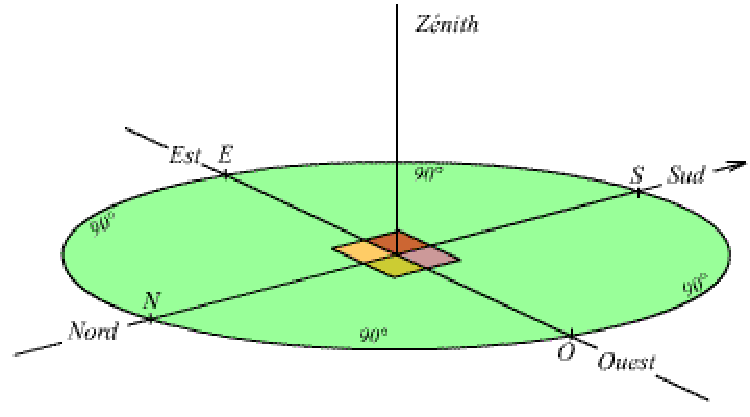
\includegraphics[width=0.4\textwidth]{position}
      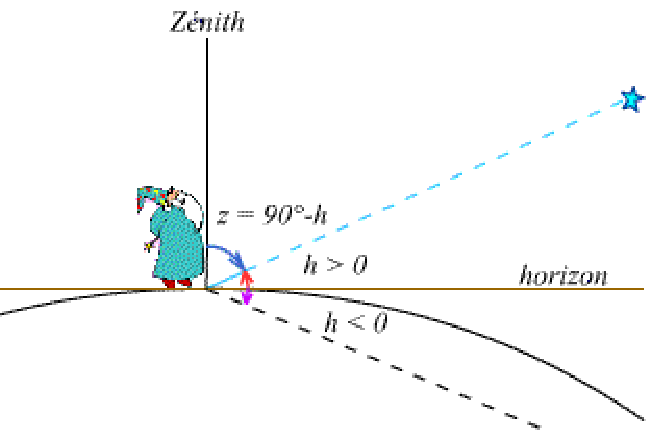
\includegraphics[width=0.4\textwidth]{position2}
    \end{center}
    \label{position}
    \label{position2}
    \caption{G.: Points cardinaux. Dr.: Horizon et distance zénithale.}
  \end{figure}
\end{Answer}

\section{Mouvement diurne}

\begin{Exercise}
  \begin{enumerate}
  \item Dans quelle direction se trouve un astre au moment de sa
    culmination en un lieu de latitude $+50\deg$?
  \item Même question pour un lieu situé à l'équateur.
  \item La hauteur d'un astre varie-t-elle au cours du mouvement
    diurne au pôle Nord?
  \end{enumerate}
\end{Exercise}

\begin{Answer}
  \begin{enumerate}
  \item Lors du mouvement diurne, la culmination d'un astre se produit
    lorsque sa hauteur est maximale.  Suivant sa position de l'objet
    sur la sphère céleste (donc sa déclinaison), l'astre passera entre
    le zénith et le pôle (Nord pour un habitant de l'hémisphère nord
    et Sud pour ...) soit entre le zénith et l'horizon opposé au pôle
    visible. À la latitude de $50\deg$, les étoiles dont la
    déclinaison est plus petite que la latitude, la culmination se
    fera du côté Sud de l'observateur.  Pour les autres étoiles, la
    culmination sera du côté Nord (Fig.~\ref{mouvementdiurne2})

    \begin{figure}[htp]
      \centering
      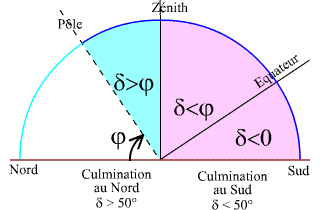
\includegraphics[width=0.3\textwidth]{mouvement_diurne2}
      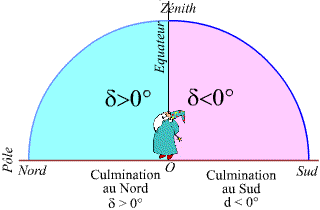
\includegraphics[width=0.3\textwidth]{mouvement_diurne3}
      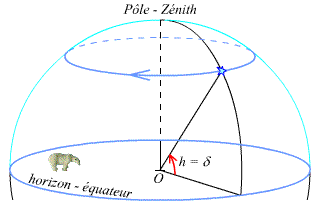
\includegraphics[width=0.3\textwidth]{mouvement_diurne4}
      \label{mouvementdiurne2}
      \label{mouvementdiurne3}
      \label{mouvementdiurne4}
      \caption{Mouvement diurne à une latitude $\phi\sim 50\deg$
        (à g.), à l'équateur ($\phi = 0$, au c.) et au pôle nord
        ($\phi = 90\deg$, à dr.).}
    \end{figure}

  \item L'équateur passant par le zénith, toutes les étoiles de
    déclinaisons positives culminent au Nord et les étoiles de
    déclinaisons négatives au Sud. Les étoiles de déclinaisons nulles
    passent au zénith (Fig.~\ref{mouvementdiurne3}).

  \item La verticale étant confondue avec l'axe du pôle, et l'horizon
    avec l'équateur, la déclinaison est égale à la hauteur de l'astre
    qui reste constante lors de la rotation diurne.  Seuls les objets
    de déclinaisons positives sont visibles. C'est pourquoi le Soleil
    dans son mouvement apparent durant l'année donne 6 mois
    consécutifs de jour et 6 mois consécutifs de nuit
    (Fig.~\ref{mouvementdiurne4}).
  \end{enumerate}
\end{Answer}

\begin{Exercise}[Mouvement diurne des étoiles]
  \begin{enumerate}
  \item Comment varie l'azimut d'un astre au cours du mouvement
    diurne, en un lieu de latitude $50\deg$ ? Et aussi $-50\deg$ de
    latitude. Sur la Fig.~\ref{mouvementdiurne}, on a représenté la
    situation en un lieu de l'hémisphère Sud (latitude = $-50\deg$) ;
    $P$ est alors en-dessous de l'horizon et $P'$ est au-dessus.

    \begin{figure}[htp]
      \centering
      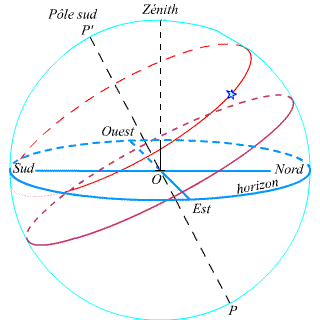
\includegraphics[width=0.5\textwidth]{mouvement_diurne}
      \label{mouvementdiurne}
      \caption{Rotation d'une étoile vue de l'hémisphère sud (latitude =
        $-50\deg$).}
    \end{figure}

  \item Les astres se lèvent-ils du côté de l'Est et se couchent-ils
    du côté de l'Ouest aussi bien dans l'hémisphère Nord que dans
    l'hémisphère Sud?
  \item Dans quelle direction géographique un astre culmine-t-il en un
    lieu de latitude $-50\deg$ ?
  \item Le mouvement diurne est-il observé dans le même sens pour un
    observateur de l'hémisphère Nord ou un observateur de l'hémisphère
    Sud?
  \end{enumerate}
\end{Exercise}

\begin{Answer}
  \begin{enumerate}
  \item
    \begin{description}
    \item[Observateur de l'hémisphère Nord (latitude $+50\deg$)] On
      n'envisagera que le cas des étoiles visibles par l'observateur,
      c'est-à-dire celles dont $\delta > -(\pi/2 - \phi)$. Deux
      critères sont a envisager :
      \begin{itemize}
      \item l'étoile a une déclinaison plus grande que la latitude
        $\delta>\phi$ ou $\delta<\phi$
      \item l'étoile est circumpolaire $\delta > \pi/2 - \phi$
      \end{itemize}
      Par la première condition, si $\delta<\phi$, l'azimut de
      l'étoile varie de 0 à $360\deg$, sinon, son azimut oscille
      entre une valeur comprise $\alpha$ entre 90 et $180\deg$
      suivant sa position au passage au méridien et
      $360\deg-\alpha$. L'étoile oscille donc entre $\alpha$,
      $180\deg$ et $360\deg-\alpha$.

      Le deuxième critère (circumpolarité) indique si l'étoile a un
      lever ou un coucher, son azimut varie alors entre les positions
      des levers et couchers et celles définies par le premier
      critère.

      L'observateur orienté vers le Nord voit tourner les étoiles dans
      le sens direct autour du pôle Nord.

    \item[Observateur de l'hémisphère Sud (latitude $-50\deg$)] Les
      mêmes critères s'appliquent pour les limitations des azimuts et
      des levers et couchers, à la différence que l'azimut va osciller
      autour de la valeur $0\deg$ et que regardant le pôle Sud, il
      verra tourner les étoiles dans le sens rétrograde
      (Fig.\ref{mouvementdiurne}).
    \end{description}
  \item Oui. Que l'on soit dans l'hémisphère Nord ou Sud, le sens de
    rotation de la Terre est le même. Les objets apparaissent à l'Est
    et se couchent à l'Ouest.

  \item Au Nord si sa déclinaison est plus grande que la latitude,
    autrement au Sud (Voir exercice 1 du même chapitre).

  \item Non (Voir exercice 4 du chapitre II).
  \end{enumerate}
\end{Answer}

\begin{Exercise}[Coordonnées horaires d'un astre]
  \begin{enumerate}
  \item Quelle est la relation entre la déclinaison et la distance
    polaire?
  \item Quelles sont les coordonnées horaires des quatre points
    cardinaux en un lieu de latitude $\phi$?
  \item Que vaut la déclinaison du zénith en fonction de la latitude
    du lieu?
  \end{enumerate}
\end{Exercise}

\begin{Answer}
  \begin{enumerate}
  \item Comme son nom l'indique, la distance polaire est l'angle entre
    la direction du pôle nord et la direction de l'objet, donc
    $p=90\deg-\delta$

  \item Table~\ref{tbl:coordonnees_horaire} et
    Fig.~\ref{coordonneeshoraire}

    \begin{center}
      \begin{tabular}{|c|c|c|}
        \hline
        Points cardinaux & Angle horaire & Déclinaison \\ \hline
        Sud   & 0h  & -(90 - $\phi$) \\ \hline
        Ouest & 6h  & 0 degré \\ \hline
        Nord  & 12h & 90 - $\phi$ \\ \hline
        Est   & 18h & 0 degré \\ \hline
      \end{tabular}
      \label{tbl:coordonnees_horaire}
    \end{center}

    \begin{figure}[htp]
      \centering
      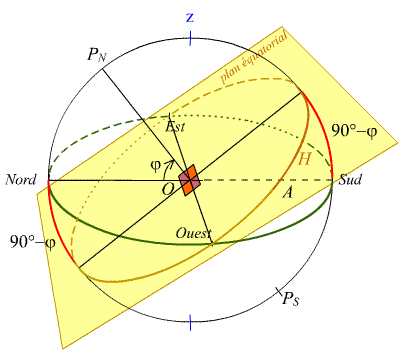
\includegraphics[width=0.45\textwidth]{coordonnees_horaire}
      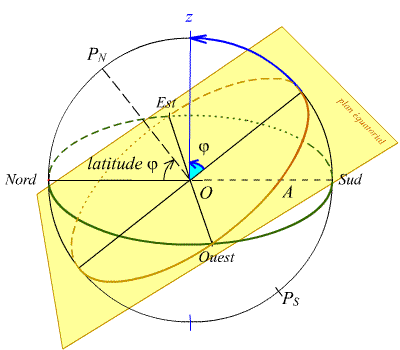
\includegraphics[width=0.45\textwidth]{coordonnees_horaire2}
      \label{coordonneeshoraire}
      \label{coordonneeshoraire2}
      \caption{Coordonnées horaires des points cardinaux (à g.) et du
        zénith (à dr.).}
    \end{figure}

  \item La déclinaison du zénith vaut la latitude (positive pour
    l'hémisphère Nord et négative pour l'hémisphère Sud), cf. Fig.
    \ref{coordonneeshoraire2}.
  \end{enumerate}
\end{Answer}

\begin{Exercise}[Coordonnées équatoriales]
  \begin{enumerate}
  \item Une étoile traverse le méridien sud à une hauteur de
    $85\deg$, et le méridien nord à $45\deg$. Trouver la
    déclinaison de l'étoile et la latitude de l'observateur.
  \item Où ces affirmations sont-elles vraies?
    \begin{enumerate}
    \item Castor ($\alpha$-Gem, déclinaison $+31\deg54'$) est
      circumpolaire.
    \item Bételgeuse ($\alpha$-Ori, $7\deg24'$) culmine au
      zénith.
    \item $\alpha$-Cen ($-60\deg46'$) s'élève à une hauteur de
      $20\deg$ au méridien.
    \end{enumerate}
  \end{enumerate}
\end{Exercise}

\begin{Answer}
  \begin{enumerate}
  \item L'étoile tournant autour de la direction du pôle, les deux
    directions $OA$ et $OB$ des passages supérieur et inférieur, sont
    symétriques par rapport à l'axe $OP$. L'angle $\alpha$ égale
    l'angle $\beta$ et
    $$
    \alpha + \beta+180\deg - 45\deg -85\deg = 50\deg
    \quad\to\quad
    \alpha=\beta=25\deg
    $$
    $\alpha$ et $\beta$ sont tous deux les compléments de la
    déclinaison de l'étoile:
    $$
    \beta+\delta = 90\deg
    \quad\to\quad
    \delta=65\deg
    $$
    On calcule la latitude qui vaut la hauteur du pôle au dessus de
    l'horizon: $\phi=\alpha+45\deg=70\deg$.

    \begin{figure}[htp]
      \centering
      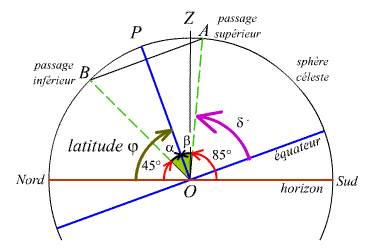
\includegraphics[width=0.5\textwidth]{coordonnees_horaire3}
      \label{coordonneeshoraire3}
      \caption{Coordonnées horaires.}
    \end{figure}

  \item
    \begin{description}
    \item[Castor (Gem, $\delta = +31\deg56'$) circumpolaire]
      L'étoile sera juste circumpolaire, c'est-à-dire passera tangent
      à l'horizon Nord, si sa déclinaison est le complément de la
      latitude.  Pour toute latitude plus grande, l'étoile sera plus
      élevée sur l'horizon et ne disparaîtra pas derrière celui-ci
      (Fig \ref{castor}): $\phi>=90\deg-\delta$
      \begin{figure}[htp]
        \centering
        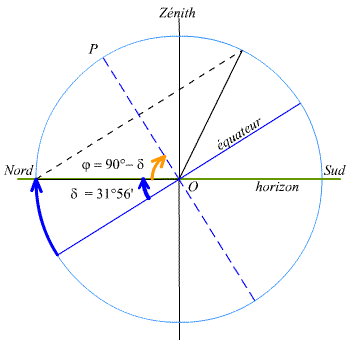
\includegraphics[width=0.3\textwidth]{castor}
        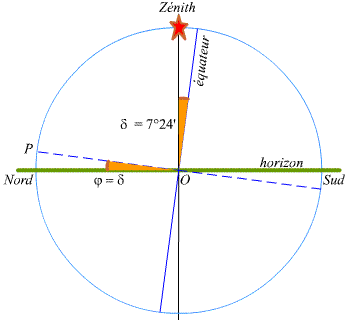
\includegraphics[width=0.3\textwidth]{betelgeuse}
        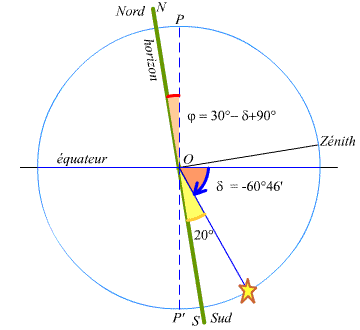
\includegraphics[width=0.3\textwidth]{cen}
        \label{castor}
        \label{betelgeuse}
        \label{cen}
        \caption{Castor (à g.), Bételgeuse (au c.), et
          $\alpha$-Cen. (à dr.).}
      \end{figure}

    \item[Bételgeuse (Ori, $\delta = +7\deg24'$) culmine au zénith]
      Si l'étoile est au moment de sa culmination au zénith
      (nécessairement), sa déclinaison est égale à la latitude
      (Fig.~\ref{betelgeuse}): $\phi=7\deg24'$

    \item[$\alpha$-Cen ($\delta = - 60\deg46'$) s'élève à une
      hauteur de $+20\deg$] À son passage supérieur, l'étoile se
      trouve dans la configuration Fig.~\ref{cen}.  La latitude est
      l'angle $PON$ qui est égal à $P'OS$. En appliquant la relation
      de Chasles entre $P'OS$ la hauteur de l'astre $20\deg$ et la
      déclinaison, on obtient: $P'OS=90\deg+\delta-20\deg$ d'où
      $\phi = 9\deg14'$
    \end{description}
  \end{enumerate}
\end{Answer}

\section{Mouvement du Soleil}

\subsection{Année sidérale, année tropique }

\begin{Exercise}[Mouvement du Soleil, jour solaire]
  \begin{enumerate}
  \item Que valent la hauteur maximale et la hauteur minimale du
    Soleil en chacun des lieux considérés : $50\deg$, $75\deg$,
    $10\deg$, $20\deg$?

  \item À quelle condition doit satisfaire la latitude d'un lieu pour
    que le Soleil n'ait ni lever ni coucher?

  \item Comment comprendre l'expression « soleil de minuit » ?

  \item À quelle condition doit satisfaire la latitude d'un lieu pour
    que le Soleil puisse passer à son zénith?

  \item Comment comprendre l'expression « tropique du Cancer » et «
    tropique du Capricorne » ? on pourra discuter cette question, en
    particulier, en consultant une carte céleste.
  \end{enumerate}
\end{Exercise}

\begin{Answer}
  \begin{enumerate}
  \item Inclinaison de l'écliptique sur l'équateur:
    $\epsilon=23\deg27'$. On détermine les relations qui relient la
    latitude $\phi$, les hauteurs minimum et maximum avec les deux
    positions du Soleil en déclinaison $\pm \epsilon$.
    \begin{itemize}
    \item Position solstice hiver: $SOm = SOE - \epsilon =
      (90\deg-\phi) -\epsilon$
    \item Position solstice été: $SOm = SOE + \epsilon =
      (90\deg-\phi) +\epsilon$
    \end{itemize}
    ou le supplément si le Soleil sous les tropiques est passé de
    l'autre côté.
    \begin{center}
      \begin{tabular}{|c|c|c|c|c|}
        \hline
        Latitude $\epsilon$ & $50\deg$ & $75\deg$ & $10\deg$ &
        $-20\deg$ \\
        \hline
        Hauteur max. & $67\deg27'$ & $38\deg27'$ & $90\deg$ &
        $90\deg$ \\
        \hline
        Hauteur min. & $16\deg33'$ & $-08\deg27'$ & $56\deg33'$
        & $46\deg33'$ \\
        \hline
      \end{tabular}
    \end{center}
    Attention aux positions entre les tropiques, le Soleil au solstice
    d'été pour les latitudes nord (solstice d'hiver pour les latitudes
    sud) est passé au Sud (au Nord) et de ce fait est plus bas que le
    jour où il passe au zénith au méridien (Fig.~\ref{mvtsolaire}).

    \begin{figure}[htp]
      \centering
      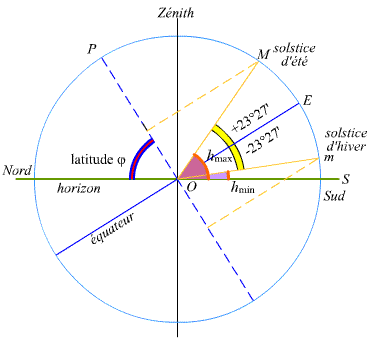
\includegraphics[width=0.5\textwidth]{mvt_soleil}
      \label{mvtsolaire}
      \caption{}
    \end{figure}

  \item Ceci se produit dans l'hémisphère nord en été quand le Soleil
    a une déclinaison suffisamment positive. On appelle ce phénomène
    le « soleil de minuit ». Sur la figure ci-contre (cas de
    l'hémisphère Nord), lorsque au passage inférieur, l'angle $NOD$
    est positif, le Soleil ne se couche pas, son mouvement est
    circumpolaire.
    \begin{eqnarray*}
      NOD = NOE' + E'OD > 0 \\
      90\deg - \phi < \delta_{soleil} \\
      \phi > 90\deg - \delta_{soleil}
    \end{eqnarray*}
    Au jour des solstices ($\delta_{soleil} = \pm 23\deg27'$) il
    suffit d'être à une latitude $\phi > 66\deg33'$ (en été pour
    l'hémisphère Nord) ou $\phi < - 66\deg33'$ (en hiver pour
    l'hémisphère Sud) ; les lieux de latitude $\phi$ égale à $\pm
    66\deg33'$ définissent sur le globe terrestre les parallèles
    appelés « cercles polaires » (respectivement boréal et austral)
    (Fig.~\ref{mvtsolaire2}).

    \begin{figure}[htp]
      \centering
      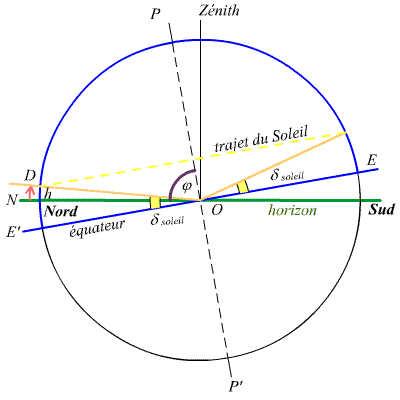
\includegraphics[width=0.5\textwidth]{mvt_soleil2}
      \label{mvtsolaire2}
      \caption{}
    \end{figure}

  \item Vers les pôles, lors de son passage inférieur dans le plan
    méridien, le Soleil est au-dessus de l'horizon et son angle
    horaire ayant augmenté de $180\deg$ depuis sa culmination (par
    définition, il s'agit alors de « midi », 0h temps solaire) vaut
    12h, cela correspond bien à « minuit ». À noter que le Soleil de
    minuit s'observe au Nord dans l'hémisphère boréal et au Sud dans
    l'hémisphère Sud.

  \item Pour que le Soleil passe au zénith, il faut que la déclinaison
    du zénith (qui est aussi la latitude du lieu) soit égale à celle
    du Soleil; comme cette dernière ne peut varier qu'entre
    $+23\deg27'$ et $-23\deg27'$, les lieux en question sont ceux
    de latitude comprise entre $-23\deg27'$ et $+23\deg27'$. Le
    Soleil passe au zénith de ces lieux deux fois dans le cours d'une
    année, au printemps et en été dans l'hémisphère Nord et en automne
    et en hiver dans l'hémisphère Sud. Les zones de la Terre qui
    correspondent à cette propriétés sont appelées les zones
    tropicales car situées entre le tropique nord du Cancer et le
    tropique sud du Capricorne.

  \item Pour les lieux de latitude égale à $+23\deg27'$ et
    $-23\deg27'$, le Soleil passe au zénith au moment des
    solstices. Ces lieux définissent sur le globe terrestre les
    parallèles appelés « tropiques » (du Cancer pour l'hémisphère Nord
    et du Capricorne pour l'hémisphère Sud). Si l'on se reporte à une
    carte du ciel, on voit qu'au moment des solstices le Soleil se
    trouve dans la direction de la constellation des Gémeaux (été) ou
    du Sagittaire (hiver). Il faudrait donc désigner les lieux en
    question par les noms : « tropique des Gémeaux » au lieu de
    tropique du Cancer et de même « tropique du Sagittaire » au lieu
    de tropique du Capricorne. L'appellation en usage a été définie il
    y a environ 3000 ans à une époque où le point gamma était dans la
    direction de la constellation du Bélier ; au solstice d'été le
    Soleil était bien dans la direction du Cancer et au solstice
    d'hiver dans la direction du Capricorne. Ce glissement est produit
    par la précession des équinoxes au rythme de $360\deg$ pour 26
    000 ans, ce qui donne un effet de $42\deg$, (soit environ un
    angle de 3h) sur 3 000 ans, comme on peut le lire sur la carte.
\end{enumerate}
\end{Answer}

\end{document}

%%% Local Variables:
%%% mode: latex
%%% TeX-PDF-mode : 0
%%% ispell-local-dictionary: "francais"
%%% End:
"' pour une version sans
% les solutions.

\documentclass[a4paper,10pt]{report}

% PREAMBULE ==============================

\usepackage[T1]{fontenc}
\usepackage[utf8]{inputenc}
\usepackage[ec]{aeguill}
\usepackage{ae}
\usepackage[cm]{fullpage}
\usepackage[francais]{babel}
\usepackage{amsmath}
\usepackage{multirow}

\usepackage[pdftex]{graphicx}
\graphicspath{{./Figures/}}

%\usepackage[backref,colorlinks=true,breaklinks=true,
%a4paper,bookmarks=false,linktocpage=true]{hyperref}
\usepackage[colorlinks=true]{hyperref}
\hypersetup{
  pdftitle   = Fascicule de TD,
  pdfauthor  = Astro L2,
  pdfsubject = Astrophysique,
}

% Définition de l'environnement 'Exercise'
\newcounter{noexo}
\setcounter{noexo}{0}
\newenvironment{Exercise}[1][]{%
  \stepcounter{noexo}
  \medskip\noindent\textbf{Exercice~\thenoexo~:~#1}
  \medskip\par
  \addcontentsline{toc}{subsubsection}{Exercice~\thenoexo~:~#1}
}{}

% Définition de l'environnement 'Answer'
\usepackage[usenames,dvipsnames]{color}
\usepackage{comment}
\specialcomment{Answer}{%
  \begingroup
  \sffamily\color{CadetBlue}
  \medskip\noindent\textbf{Corrigé :~}
  }{%
  \endgroup}

% Inclusion ou non des corrigés
\ifdefined\sanscorrige
  \message{Fascicule sans solutions}%
  \excludecomment{Answer} % Remove answers
\else
  \message{Fascicule *AVEC* solutions}%
\fi

% Définitions locales
\renewcommand{\d}{\ensuremath{\mathrm{d}}}
\newcommand{\UA}{\ensuremath{\textrm{UA}}}
\renewcommand{\deg}{\ensuremath{^{\circ}}}
\renewcommand{\vec}[1]{\ensuremath{\boldsymbol{#1}}}
\renewcommand{\u}[1]{\ensuremath{\mathrm{#1}}} % Unités

% PAGE DE TITRE ET PREAMBULE ==============================

\makeatletter
\def\thickhrulefill{\leavevmode \leaders \hrule height 1pt\hfill \kern \z@}
\renewcommand{\maketitle}{\begin{titlepage}%
    \let\footnotesize\small
    \let\footnoterule\relax
    \parindent \z@
    \reset@font
    \null
    \begin{center}
      \huge \bfseries \@title
      \ifdefined\sanscorrige
      \else
      \\\textcolor{red}{avec solutions}
      \fi
    \end{center}
    \hrule height 1pt
    \begin{flushright}
      Université Claude Bernard Lyon1 \\
    \end{flushright}
    \vfil
    \vfil
    \begin{figure}[htp]
      \centering
      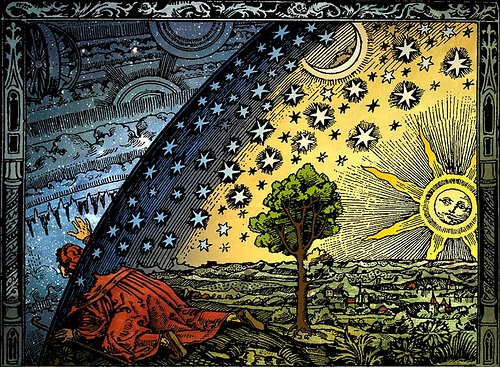
\includegraphics[width=0.8\textwidth]{flammarion}
      \caption{La gravure sur bois dite « de Flammarion »}
    \end{figure}
    \begin{center}
    \vfil
      {\Large \@author} \\[1em]
      {\large \@date}
    \end{center}
  \end{titlepage}%
  \setcounter{footnote}{0}%
}
\makeatother

\title{Fascicule de TD}
\date{Université Lyon 1}
\author{Astrophysique pour la licence}

\begin{document}

\maketitle

% 2: Down to subsection (no exercices)
% 3: Down to subsubsection (exercices)
\setcounter{tocdepth}{2}
\tableofcontents

\newpage

% EXERCICES ET SOLUTIONS ==============================

\chapter{Vie des étoiles}

\section{La lumière des étoiles}

\subsection{Notion de photométrie}

\begin{Exercise}[Dilution du flux avec la distance]
  Réécrire la relation entre la luminosité d'une étoile et le flux
  observé (équation 2.4) dans le cas où la luminosité $L(t)$ dépend du
  temps (par exemple parce que l'étoile est variable) et donc le flux
  observé $F(D,t)$ dépend du temps et de la distance.
\end{Exercise}

\begin{Answer}
  Lorsque la luminosité $L(t)$ de l'étoile dépend du temps, les
  variations de luminosité mettent un temps $D/c$ pour parvenir à un
  observateur situé à une distance $D$ ($c$ étant la vitesse de la
  lumière). Dans ce cas la relation (2.4) devient: $L(t) = 4 \pi D^2
  F(D,t-D/c) $.
\end{Answer}

\subsection{Photosphère et température effective}

\begin{Exercise}[Température effective d'une étoile]
  Calculer la température effective du Soleil à partir de sa
  luminosité $L_{\odot}\approx 3.83\times 10^{26}$~W et de son rayon
  $R_{\odot}\approx 6.96 \times 10 ^{8}$~m.
\end{Exercise}

\begin{Answer}
  En appliquant l'équation :
  $$
  T_e = \left( \frac{L}{4 \pi \sigma R^2_p} \right)^{1/4}
  $$
  avec la constante de Stefan $\sigma = 5.67 \times
  10^{-8}$~\u{Wm^{-2}K^{-4}}, on trouve la température effective du
  Soleil $T_\odot \approx 5770$~K.
\end{Answer}

\subsection{Système de magnitudes}

\begin{Exercise}[Indices de couleur]
  Les deux composantes de l'étoile $\alpha$ du Centaure située à
  1,32~pc de distance ont des magnitudes visuelles (magnitude
  apparente dans la bande $V$) de 0,30 et 1,70. On demande :
  \begin{enumerate}
  \item Le rapport des flux des deux étoiles dans la bande $V$.
  \item La magnitude visuelle globale du système.
  \item La correction qu'il faut apporter aux magnitudes apparentes de
    ce système pour obtenir les magnitudes absolues.
  \end{enumerate}
\end{Exercise}

\begin{Answer}
  On rappelle que la magnitude apparente $m$ est liée au flux $F$ par
  $m = -2,5 \log_{10}(F / F_{0})$.
  \begin{enumerate}
  \item Le rapport des flux des deux composantes de $\alpha$ du
    Centaure dépend de la différence de magnitudes et vaut :
    $$
    F_2 / F_1 = 10^{(m_{1} - m_{2})/2,5} = 0,28
    $$
  \item Pour obtenir la magnitude visuelle globale du système $m_{tot}$,
    il faut calculer le flux total (les puissances émises par les deux
    composantes s'ajoutent) :
    $$
    m_{tot} = -2,5 \log(F_{1} / F_{0} + F_{2} / F_{0})
    $$
    donc
    $$
    m_{tot}= -2,5 \log(10^{-m_{1}/2,5} + 10^{-m_{2}/2,5}) = 0.04
    $$
  \item La correction qu'il faut apporter aux magnitudes apparentes
    $m$ de ce système pour obtenir les magnitudes absolues $M$ vaut:
    $$
    m - M = 5 \log(D/10 \u{pc}) = -4,4
    $$
  \end{enumerate}
\end{Answer}

\section{Évolution stellaire}

\subsection{Formation des étoiles}

\begin{Exercise}
  Quelle est la source de l'énergie rayonnée par:
  \begin{enumerate}
  \item une proto-étoile?
  \item une étoile?
  \item une naine brune?
  \end{enumerate}
\end{Exercise}

\begin{Answer}
  L'énergie rayonnée provient de:
  \begin{enumerate}
  \item l'énergie gravitationnelle pour une proto-étoile ;
  \item l'énergie produite par les réactions nucléaires pour une
    étoile (fusion de H sur la séquence principale, fusion de He ou de
    C et O ensuite, selon la masse de l'étoile) ;
  \item l'énergie gravitationnelle pour une naine brune, qui continue
    à se contracter, ne passant jamais de la proto-étoile à l'étoile.
  \end{enumerate}
\end{Answer}

\subsection{Séquence principale}

\begin{Exercise}
  Quel est le phénomène marquant:
  \begin{enumerate}
  \item le début de la séquence principale?
  \item sa fin?
  \end{enumerate}
\end{Exercise}

\begin{Answer}
  La séquence principale débute quand les réactions de fusion de
  l'hydrogène s'allument dans le coeur de la proto-étoile, et se
  termine lorsque la fusion de l'hydrogène cesse au centre (elle peut
  continuer dans une couche autour d'un noyau d'hélium ou cesser dans
  toute l'étoile selon sa masse).
\end{Answer}

\subsection{Évolution post-SP}

\begin{Exercise}[Étoile de $M > 5 M_{\odot}$]
  Que se passe-t-il si un combustible s'épuise au centre d'une étoile?
\end{Exercise}

\begin{Answer}
  Quand un combustible s'épuise au centre d'une étoile, les réactions
  de fusion de cet élément cessent dans le coeur, mais peuvent
  continuer autour, dans une couche où le combustible est toujours
  présent. Au centre, il n'y a plus de production d'énergie pour
  soutenir le coeur, la gravité l'emporte et le coeur se
  contracte. Cette contraction provoque une augmentation de
  température qui, si elle est suffisante (cela dépend de la masse de
  l'étoile), permet d'allumer de nouvelles réactions nucléaires ayant
  pour combustible le produit des réactions précédentes.
\end{Answer}

\section{Classification spectrale}

\subsection{Mesures des distances}

\subsubsection{Parallaxe trigonométrique}

\begin{Exercise}
  Relier l'incertitude sur la distance $\Delta d$ à celle sur la
  parallaxe $\Delta p$.
\end{Exercise}

\begin{Answer}
  Il existe deux méthodes pour trouver le résultat demandé:
  \begin{itemize}
  \item En différenciant l'équation $d = a/p$, on obtient $\d d =
    -(a/p^2)\d p$, d'où l'incertitude en prenant la valeur absolue:
    $$
    \Delta d = \frac{a}{p^2}\Delta p = \frac{d}{p}\Delta p
    $$
    On a finalement
    $$
    \frac{\Delta d}{d} = \frac{\Delta p}{p}
    $$

  \item On peut également prendre le logarithme de l'équation $d =
    a/p$, ce qui donne $\ln~d = \ln~a - \ln~p$, puis on différencie:
    $\d\ln~d = -\d\ln~p$, soit $\d d/d = -\d p/p$. En prenant la
    valeur absolue, on retrouve le résultat sur l'incertitude:
    $$
    \frac{\Delta d}{d} = \frac{\Delta p}{p}
    $$
  \end{itemize}
\end{Answer}

\begin{Exercise}
  Imaginons deux missions spatiales: FAME et GAIA. Quelles seraient
  les précisions obtenues à une distance de 100~pc? de 1000~pc?  À
  quelle distance aura-t-on une erreur de 100\%?

  On donne les incertitudes absolues sur les parallaxes pour chaque
  satellite:
  \begin{itemize}
  \item $\Delta p=50~\mu as$ pour FAME et
  \item $\Delta p=4~\mu as$ pour GAIA.
  \end{itemize}
\end{Exercise}

\begin{Answer}
  Les étoiles situées à $d=100$~pc ont une parallaxe
  $p=1/100=0,01''=10$~mas. La précision obtenue avec FAME sera de
  $$
  \frac{\Delta d}{d} = \frac{\Delta p}{p} = \frac{50 \times
    10^{-6}}{10^{-2}} = 5 \times 10^{-3} = 0.5 \%
  $$
  et de
  $$
  \frac{\Delta d}{d} = \frac{\Delta p}{p} = \frac{4 \times
    10^{-6}}{10^{-2}} = 4 \times 10^{-4} = 0.04 \%
  $$
  avec GAIA.

  Pour des étoiles à $d=1000$~pc, $p=1$~mas, et les précisions
  deviennent 10 fois moins bonnes: 5\% avec FAME et 0,4\% avec GAIA.

  On aura une erreur de 100\% quand $\Delta d =d$, soit $\delta p =
  p$. La distance correspondante s'obtient donc par
  $$
  d = \frac{1}{p} = \frac{1}{50 \times 10^{-6}} = 20~\u{kpc}
  \quad\text{avec FAME}
  $$
  et
  $$
  d = \frac{1}{p} = \frac{1}{4 \times 10^{-6}} = 250~\u{kpc}
  \quad\text{avec GAIA}
  $$
\end{Answer}


\begin{Exercise}
  Le tableau suivant donne la magnitude apparente $m_V$ et la
  parallaxe $p$ de trois étoiles. Calculer leur distance $d$ avec son
  incertitude, l'erreur relative sur la distance $\Delta d / d$ et
  leur magnitude absolue $M_V$.
  \begin{center}
    \begin{tabular}{|c|c|c|c|}
      \hline
      & $\alpha$ CMa Sirius & $\alpha$ Tau Aldebaran & $\alpha$ Ori
      Bételgeuse \\
      \hline
      $m_V$ & -1.47 & 0.85 & 0.58 \\
      \hline
      $p$ (mas) & 379.2 $\pm$ 1.6 & 50.1 $\pm$ 1.0 & 7.6 $\pm$ 1.6 \\
      \hline
      $d$ (pc) &   &   &  \\
      \hline
      $\Delta d / d$ &   &   &  \\
      \hline
      $M_V$ &   &   &  \\
      \hline
    \end{tabular}
  \end{center}
\end{Exercise}

\begin{Answer}
  \begin{center}
    \begin{tabular}{|c|c|c|c|}
      \hline
      & $\alpha$ CMa Sirius & $\alpha$ Tau Aldebaran & $\alpha$ Ori
      Bételgeuse \\
      \hline
      $m_V$ & -1.47 & 0.85 & 0.58 \\
      \hline
      $p$ (mas) & 379.2 $\pm$ 1.6 & 50.1 $\pm$ 1.0 & 7.6 $\pm$ 1.6 \\
      \hline
      $d$ (pc) &  \color{red}{2.64 $\pm$ 0.01} &  \color{red}{20.0
        $\pm$ 0.4}  & \color{red}{130 $\pm$ 30} \\
      \hline
      $\Delta d / d$ & \color{red}{0.4\%}  & \color{red}{2\%}  &
      \color{red}{23\%} \\
      \hline
      $M_V$ & \color{red}{1.42}  & \color{red}{-0.65}  &
      \color{red}{-4.99} \\
      \hline
    \end{tabular}
  \end{center}

  Étant donné la forme de la relation donnant la distance $d$ à partir
  de la parallaxe $p$, leurs incertitudes relatives sont égales, ce
  qui permet d'avoir immédiatement $\Delta d / d$. Ces résultats
  illustrent bien la diminution de la précision lorsque la distance
  augmente.

  La magnitude absolue s'obtient par la relation $M_V = m_V - 5~\log~d
  + 5$.
\end{Answer}


\begin{Exercise}[Méthode du point convergent]
  On veut déterminer la distance de l'amas des Pléiades par la méthode
  du point convergent.
  \begin{itemize}
  \item L'étude des trajectoires des étoiles de l'amas sur plusieurs
    années a permis de situer le point convergent à $\theta = 67,9 \pm
    0,6\deg$ de la direction de l'amas.
  \item L'observation du spectre de l'étoile Alcyone, faisant partie
    de cet amas, a permis de mesurer sa vitesse radiale $v_r = 10,1
    \pm 0,3$~\u{km.s^{-1}}.
  \item Le mouvement propre apparent de cette même étoile vaut $\mu =
    47,3 \pm 0,8$~\u{mas.an^{-1}}.
  \end{itemize}
  Déterminer la distance de l'amas. Attention aux unités !
\end{Exercise}

\begin{Answer}
  Dans la formule donnant la distance de l'amas, il faut bien faire
  attention à exprimer l'angle $\mu$ en radians et à utiliser les
  mêmes unités de distance et de temps pour les autres grandeurs.
  \begin{itemize}
  \item $\mu = 47,3 \pm 0,8~\u{mas.an^{-1}} = (2,29 \pm 0,04) \times
    10^{-7}~\u{rad.an^{-1}}$
  \item $v_r = 10,1 \pm 0,3~\u{km.s^{-1}} = (1,02 \pm 0,03) \times
    10^{-5}~\u{pc.an^{-1}}$
  \item $\theta = 67,9 \pm 0,6\deg = 1,19 \pm 0,01$~rad
  \item On a donc $tan \theta= 2,50 \pm 0,07$.
  \item Finalement: $d = 111 \pm 8$~pc
  \end{itemize}
\end{Answer}

\subsection{Classification stellaire}

\begin{Exercise}[Types spectraux]
  Donner approximativement le type spectral des étoiles dont le flux
  est maximal aux longueurs d'onde suivantes: 300~nm, 500~nm, et
  1,2~$\mu$m.  Peut-on déterminer la classe de luminosité?

  Rappel de la loi de Wien: $\lambda_{\max} T = 2898$~\u{\mu m.K}.
\end{Exercise}

\begin{Answer}
  La loi de Wien permet de déterminer la température effective de
  chaque étoile, et ainsi d'en déduire une valeur approximative du
  type spectral. Ici seulement la première lettre est accessible, la
  détermination du chiffre suivant nécessiterait un tableau plus
  précis donnant les correspondances entre les sous-types et la
  température effective.
  \begin{center}
    \begin{tabular}{|c|c|c|}
      \hline
      $\lambda_m$ & $T_{eff}(K)$ & Type spectral \\
      \hline
      300 nm & \color{red}{9660} & \color{red}{A}  \\
      \hline
      500 nm & \color{red}{5796} & \color{red}{G} \\
      \hline
      1.2 $\mu m$ &  \color{red}{2415} &  \color{red}{M} \\
      \hline
    \end{tabular}
  \end{center}
  On ne peut pas déterminer la classe de luminosité grâce à la
  longueur d'onde du maximum du flux. Pour ceci, il faudrait connaître
  soit la luminosité de l'étoile, soit sa gravité de surface, soit son
  rayon.
\end{Answer}

\begin{Exercise}[Diagramme HR]
  Classer par ordre de température effective croissante, puis de rayon
  croissant, et enfin de luminosité croissante les étoiles de types
  spectraux suivants: M5III, O2V, K7I, A0VII.
\end{Exercise}

\begin{Answer}
  La séquence OBAFGKM décrit les types spectraux dans le sens des
  $T_{eff}$ décroissantes, on aura donc dans le sens des $T_{eff}$
  croissantes: \textcolor{red}{M5III}, \textcolor{red}{K7I},
  \textcolor{red}{A0VII}, et \textcolor{red}{O2V}.

  La classe de luminosité définit des groupes d'étoiles de rayon
  différent, on aura donc dans l'ordre croissant:
  \textcolor{red}{A0VII}, \textcolor{red}{O2V},
  \textcolor{red}{M5III}, et \textcolor{red}{K7I}.

  Enfin, l'examen du diagramme HR montre qu'une étoile chaude de la
  séquence principale peut être plus lumineuse qu'une sous-géante
  froide, et on aura dans le sens des luminosités croissantes:
  \textcolor{red}{A0VII}, \textcolor{red}{M5III},
  \textcolor{red}{O2V}, et \textcolor{red}{K7I}.

  Ceci montre que le terme « classe de luminosité » peut être source
  d'erreur.
\end{Answer}

\subsection{Mesure des rayons}

\begin{Exercise}[Interférométrie]
  Le tableau suivant donne le diamètre apparent $\theta_*$ de quelques
  étoiles, mesuré par interférométrie. Calculer leur rayon $R$ (on
  rappelle les distances déterminées dans un exercice précédent) et, à
  l'aide de ce résultat, attribuer à chaque étoile sa classe de
  luminosité parmi les suivantes: I, III, V.

  \begin{center}
    \begin{tabular}{|c|c|c|c|}
      \hline
      & $\alpha$ CMa Sirius & $\alpha$ Tau Aldebaran & $\alpha$ Ori
      Bételgeuse \\
      \hline
      $\theta_*$ (mas) & 5.89 & 24 & 67 \\
      \hline
      $p$ (mas) & 379.2 $\pm$ 1.6 & 50.1 $\pm$ 1.0 & 7.6 $\pm$ 1.6 \\
      \hline
      $d$ (pc) & 2.64  & 20  & 130 \\
      \hline
      $R (R_{\odot})$ &   &   &  \\
      \hline
      Classe de luminosité &   &   &  \\
      \hline
    \end{tabular}
  \end{center}
\end{Exercise}

\begin{Answer}
  Pour Sirius:
  \begin{itemize}
  \item Son diamètre apparent vaut $\theta_*= 5,89~\u{mas} = 2,86 \times
    10^{-8}$~rad.
  \item Son rayon vaut donc $R = \theta_* d / 2 = 3,8 \times 10^{-8}
    pc = 1,2 \times 10^9 m = 1,7R_{\odot}$.
  \end{itemize}
  Le tableau suivant donne les résultats pour les 3 étoiles:
  \begin{center}
    \begin{tabular}{|c|c|c|c|}
      \hline
      & $\alpha$ CMa Sirius & $\alpha$ Tau Aldebaran & $\alpha$ Ori
      Bételgeuse \\
      \hline
      $\theta_*$ (mas) & 5.89 & 24 & 67 \\
      \hline
      $p$ (mas) & 379.2 $\pm$ 1.6 & 50.1 $\pm$ 1.0 & 7.6 $\pm$ 1.6 \\
      \hline
      $d$ (pc) & 2.64  & 20  & 130 \\
      \hline
      $R (R_{\odot})$ & \color{red}{1.7}  & \color{red}{52}  &
      \color{red}{936} \\
      \hline
      Classe de luminosité & \color{red}{V}  & \color{red}{III}  &
      \color{red}{I} \\
      \hline
      Type spectral & A1V  & K5III  & M2I \\
      \hline
    \end{tabular}
  \end{center}
  Dans cet exemple, il est possible d'attribuer à chaque étoile sa
  classe de luminosité en utilisant le lien qui existe avec le rayon
  stellaire. Le type spectral complet est donné pour information.
\end{Answer}

\subsection{Mesure de masse}

\subsubsection{Étoiles doubles}

\begin{Exercise}
  On observe une étoile double visuelle dont le plan de l'orbite est
  perpendiculaire à la ligne de visée.
  \begin{itemize}
  \item La parallaxe de ce système est de 100~mas.
  \item La plus grande séparation angulaire entre les deux composantes
    est de $5''$, et la plus petite de $1''$.
  \item La période de révolution est de 30~ans.
  \item L'étoile primaire se trouve au foyer de l'orbite observée, car
    il n'y a pas d'effet de projection.
  \item Le compagnon est toujours observé à une distance du centre de
    gravité 5~fois plus grande que celle de l'étoile primaire.
  \end{itemize}

  Déterminer la masse de chaque composante.
\end{Exercise}

\begin{Answer}
  Les paramètres observés permettent de remonter aux données suivantes
  pour le système:
  \begin{itemize}
  \item La distance est $d = 10$~pc.
  \item La dimension angulaire du grand axe de l'orbite relative est
    de $5'' + 1'' = 6''$. Le demi-grand axe apparent est donc $\theta
    = 3''$, soit $\theta = 1,45 \times 10^{-5} rad$.
  \item Le demi-grand axe de l'orbite relative vaut donc $a = \theta d
    = 1,45 \times 10^{-4} pc = 4,49 \times 10^{12} m = 30 \UA$.
  \item La $3^{ème}$ loi de Kepler donne la somme des masses: $M1 + M2
    = 5,97 \times 10^{31} kg = 30 M_{\odot}$ .
  \item Les distances des étoiles $E_1$ et $E_2$ au centre de gravité
    $G$ vérifient $M_1 \times GE_1 = M_2 \times GE_2$. Le rapport des
    masses vaut donc $M_1 / M_2 = GE_2 / GE_1 = 5$.
  \item Finalement: $M_1 = 25M_{\odot}$ et $M_2 = 5M_{\odot}$
  \end{itemize}
\end{Answer}


\begin{Exercise}
  Le tableau suivant rappelle les caractéristiques du système binaire
  à éclipse d'Algol ($\beta$ Per):
  \begin{center}
    \begin{tabular}{|l|c|r|}
      \hline
      $p$ (mas) &  \multicolumn{2}{c|}{35.1 $\pm$ 0.9} \\
      \hline
      $d$ (pc) & \multicolumn{2}{c|}{28.6 $\pm$ 0.7} \\
      \hline
      $T$ (jours) & \multicolumn{2}{c|}{2.8674} \\
      \hline
      & A & B \\
      \cline{1-3}
      Type spectral & B8V & K2IV \\
      \hline
      R ($R_{\odot}$) & 2.74 & 3.60 \\
      \hline
    \end{tabular}
  \end{center}
  On a mesuré de plus les paramètres orbitaux suivants (on supposera
  l'orbite circulaire, ainsi le demi-grand axe de l'ellipse projetée
  est égal au rayon de l'orbite):
  \begin{center}
    \begin{tabular}{|c|c|}
      \hline
      $\theta$ (mas) & 2.283 \\
      \hline
      $\theta_2$ (pc) & 1.872 \\
      \hline
    \end{tabular}
  \end{center}
  Quelle est la séparation des deux étoiles en km? en UA? en
  $R_{\odot}$? Comparez-la à leurs rayons.

  Quelle est la masse de chacune des étoiles?
\end{Exercise}

\begin{Answer}
  \begin{itemize}
  \item Le demi-grand axe apparent de l'orbite relative est $\theta =
    2.283~mas = 1,11 \times 10^{-8}~rad$.
  \item Le demi-grand axe de l'orbite relative vaut donc $a = \theta d
    = 3,17 \times 10^{-7}~pc = 9,77 \times 10^9~m = 0,065~\UA =
    14R_{\odot}$.
  \item La 3ème loi de Kepler donne la somme des masses:
    $M_1+M_2 = 4\pi^2 a^3/GT^2 = 8,98 \times 10^{30}~kg =
    4,52M_{\odot}$.
  \item Le rapport des demi-grands axes apparents de l'orbite relative
    $\theta$ et de l'orbite absolue de l'étoile secondaire $\theta_2$
    donne le rapport des masses: $\theta_2 / \theta = a_2 / a = M_1 /
    (M_1 + M_2) = 0,82$
  \item On obtient donc les masses $M_1 = 3,71$ et $M_2 = 0,81$.
  \end{itemize}

  Le tableau suivant récapitule les données physiques du système:
  \begin{center}
    \begin{tabular}{|l|c|r|}
      \hline
      $d$ (pc) & \multicolumn{2}{c|}{28.6 $\pm$ 0.7} \\
      \hline
      $T$ (jours) & \multicolumn{2}{c|}{2.8674} \\
      \hline
      $a$ ($R_{\odot}$) &  \multicolumn{2}{c|}{\color{red}{14}} \\
      \hline
      & A & B \\
      \cline{1-3}
      Type spectral & B8V & K2IV \\
      \hline
      R ($R_{\odot}$) & 2.74 & 3.60 \\
      \hline
      M ($M_{\odot}$) & \color{red}{3.71} & \color{red}{0.81} \\
      \hline
    \end{tabular}
  \end{center}
  On remarque que l'étoile la plus grosse (B) est la moins massive et
  la moins chaude, on peut en déduire que le minimum principal a lieu
  lorsque cette dernière occulte l'étoile A, plus chaude et plus
  lumineuse.

  On constate également que la séparation des étoiles vaut un peu
  moins de 4 fois le rayon de la plus grosse, il s'agit donc d'une
  binaire serrée.
\end{Answer}

\section{Les systèmes planétaires}

\subsection{Les lois de Kepler}

\begin{Exercise}[Enoncé et rappels sur les ellipses]
  L'orbite de Pluton est très excentrique ($e=0,248$). Son demi grand
  axe vaut 39,43~unités astronomiques (L'unité astronomique est
  définie comme le demi grand axe de l'orbite de la Terre). Montrer
  que Pluton peut être plus proche du Soleil que Neptune dont le demi
  grand axe de l'orbite vaut 30,06~UA et l'excentricité 0,009.
\end{Exercise}

\begin{Answer}
  On calcule simplement les distances planète-Soleil pour les deux
  planètes à leur périhélie et à leur aphélie. Si Neptune est repérée
  par le vecteur $\vec{SN}$ et Pluton par le vecteur $\vec{SP}$, on a:
  \begin{itemize}
  \item Au périhélie:
    $$
    SN = a_n(1-e_n) = 30.06 \times (1-0.009) = 29.79~\UA
    $$
    $$
    SP = a_p(1-e_p) = 39.43 \times (1-0.248) = 29.65~\UA
    $$
  \item À l'aphélie:
    $$
    SN = a_n(1+e_n) = 30.06 \times (1+0.009) = 30.33~\UA
    $$
    $$
    SP = a_p(1+e_p) = 39.43 \times (1+0.248) = 49.21~\UA
    $$
  \end{itemize}
  On voit que, du fait de la très grande excentricité de son orbite,
  Pluton, à son périhélie, est plus proche que Neptune du Soleil.
\end{Answer}

\begin{Exercise}[Dérivation des lois de Kepler]
  Montrer que la vitesse angulaire d'un objet décrivant une orbite
  elliptique autour du Soleil augmente lorsqu'il s'en
  rapproche. Montrer que le rapport des vitesses au périhélie (point
  le plus proche du Soleil) et à l'aphélie (point le plus éloigné du
  Soleil) ne dépend que de l'excentricité de l'orbite.  Calculer ce
  rapport pour la Terre dont l'excentricité de l'orbite vaut 0,0167,
  puis pour la comète de Halley dont l'excentricité de l'orbite vaut
  0,97.
\end{Exercise}

\begin{Answer}
  \begin{enumerate}
  \item On a vu que $r^2\dot{\theta}$ est une constante. On a donc
    $\dot{\theta}=C/r^3$ et la vitesse angulaire augmente lorsque $r$
    diminue.

  \item L'expression de la vitesse est: $\vec{v} = \dot{r}\vec{i} +
    r\dot{\theta}\vec{j}$

    Le périhélie et l'aphélie correspondent à des extremum sur la
    trajectoire, c'est à dire que $\d r/\d\theta =0$ et donc,
    puisque $\dot{r} = \dot{\theta}~\d r/\d\theta$,
    $\dot{r}=0$. La vitesse s'écrit donc bien $v = r\dot{\theta}$

  \item Puisque $r^2\dot{\theta}=C$ et que $v = r\dot{\theta}$, on a
    $v = C/r$. En reprenant les résultats vus précédemment sur les
    ellipses, on trouve $r = a(1-e)$ au périhélie, et $r = a(1+e)$ à
    l'aphélie. Le rapport des vitesse $v_p$ au périhélie et $v_a$ à
    l'aphélie est donc:
    $$
    \frac{v_p}{v_a} = \frac{1+e}{1-e}
    $$
    Soit pour la Terre:
    $$
    \frac{v_p}{v_a} = \frac{1+0.0167}{1-0.0167} = 1.034
    $$
    Et pour la comète de Halley:
    $$
    \frac{v_p}{v_a} = \frac{1+0.97}{1-0.97} = 65.67
    $$
  \end{enumerate}
\end{Answer}

\begin{Exercise}
  En reprenant le raisonnement précédent, trouver l'équation de la
  trajectoire d'une planète autour du Soleil si la force de
  gravitation était en $1/r^3$ au lieu de $1/r^2$. En déduire que dans
  ce cas, vous ne seriez pas en train de vous embêter à faire cet
  exercice.
\end{Exercise}

\begin{Answer}
  On reprend l'expression de l'équation différentielle en remplaçant
  $y^2$ dans le membre de droite par $y^3$. On obtient l'équation
  suivante:
  $$
  -C^2 y^2 \left( y + \frac{d^2y}{d \theta ^2} \right) = -G(M_{\odot}
  + M_p)y^3
  $$
  Qui se simplifie par:
  $$
  -C^2 y - C^2 \frac{d^2y}{d \theta ^2} = G(M_{\odot} + M_p)y
  $$
  Qui devient, en réorganisant les différents termes:
  $$
  \frac{d^2y}{d \theta ^2} + \left[ 1 - \frac{ G(M_{\odot} + M_p)
    }{C^2} \right]y = 0
  $$
  Ou encore, en posant $\alpha = \left[ 1 - \frac{ G(M_{\odot} + M_p)
    }{C^2} \right]$
  $$
  \frac{d^2y}{d \theta ^2} + \alpha y = 0
  $$
  Il faut analyser les trois cas $\alpha < 0$, $\alpha > 0$ et $\alpha
  = 0$.
  \begin{description}
  \item[$\alpha > 0$] On pose $\epsilon = \sqrt{\left | \alpha \right |
    }$ et l'équation différentielle s'écrit alors:
    $$
    \frac{d^2y}{d \theta ^2} + \epsilon^2 y = 0
    $$
    dont la solution s'écrit simplement:
    $$
    y = K\cos(\epsilon \theta + \phi)
    $$
    donc:
    $$
    r = \frac{C}{\cos(\epsilon \theta + \phi)}
    $$
    où $C$, $\phi$ et $\epsilon$ sont des constantes. Cette équation a
    une singularité lorsque $\theta = (\pi/2 - \phi) /
    \epsilon$. Lorsque $\theta$ approchera cette valeur, la planète
    s'échappera puisqu'alors $r \to \infty$. La figure (\emph{pas
      trouvé la figure}) montre la trajectoire correspondante pour les
    valeurs des constantes suivantes: $\epsilon = 0.05$, $\phi=0$ et
    $C=1$. La planète arrive à proximité de l'étoile par une des
    branches infinies, et repart par l'autre après avoir décrit
    quelques révolutions autour de l'étoile.

  \item[$\alpha < 0$] Comme précédemment, on réécrit l'équation
    différentielle:
    $$
    \frac{d^2y}{d \theta ^2} + \epsilon^2 y = 0
    $$
    Dont la solution est:
    $$
    y = A e^{\epsilon \theta} + B e^{- \epsilon \theta}
    $$
    donc:
    $$
    r = \frac{1}{A e^{\epsilon \theta} + B e^{- \epsilon \theta}}
    $$
    On voit cette fois que lorsque $\theta$ augmente $r$ diminue
    exponentiellement. la planète s'effondrera donc sur l'étoile.

  \item[$\alpha = 0$] L'équation différentielle a la forme suivante:
    $$
    \frac{d^2y}{d \theta ^2} = 0
    $$
    Dont la solution est:
    $$
    y = A \theta + B
    $$
    donc:
    $$
    r = \frac{1}{A \theta + B}
    $$
    Ici encore, la planète s'effondrera sur l'étoile. On voit donc que
    si la loi de la gravitation était en $\frac{1}{r^3}$, il
    n'existerait pas de trajectoire fermée dans le problème à deux
    corps, et aucune planète ne pourrait graviter autour des étoiles.
  \end{description}
\end{Answer}


\begin{Exercise}
  Sachant que la Lune décrit son orbite autour de la Terre en 27,32
  jours et que le demi grand-axe de son orbite vaut 384400 km,
  calculer l'altitude d'un satellite géostationaire. On supposera que
  la masse de la Lune est négligeable par rapport à celle de la Terre
  (la Terre est environ 80 fois plus massive que la Lune).
\end{Exercise}

\begin{Answer}
  La troisième loi de Kepler, telle que nous venons de la démontrer
  s'applique bien sûr aussi pour le système Terre-Lune et on a:
  $$
  \frac{a^3_L}{T^2_L} = \frac{G(M_T + M_L)}{4\pi^2}
  $$
  Où $a_L$ est le demi grand axe de l'orbite de la Lune, $T_L$ sa
  période orbitale et $M_L$ sa masse. Puisque la masse de la Lune peut
  être négligée par rapport à celle de la Terre, cette relation s'écrit:
  $$
  \frac{a^3_L}{T^2_L} = \frac{GM_T}{4\pi^2}
  $$
  De même, pour le satellite, l'hypothèse $M_S \ll M_T$ est encore plus
  justifiée, et on a:
  $$
  \frac{a^3_S}{T^2_S} = \frac{GM_T}{4\pi^2}
  $$
  et donc:
  $$
  \frac{a^3_S}{T^2_S} = \frac{a^3_L}{T^2_L}
  $$
  La période d'un satellite géostationnaire est, par définition, de 23h56
  heures (car un satellite géostationnaire reste toujours au dessus du
  même point de la Terre dont la période de rotation est de 23h56
  heures). On a donc
  $$
  T_S = 23 \times 60 + 56 = 1435~min
  $$
  $$
  T_L = 27.3 \times 24 \times 60 = 39312~min
  $$
  et
  $$
  \frac{a^3_S}{1435^2} = \frac{384400^3}{39312^2}
  $$
  d'où l'on tire finalement:
  $$
  a_S = 42300~km
  $$
  Cette valeur correspond à la distance entre le centre de la Terre et
  le satellite. L'altitude du satellite est donc:
  $$
  a_S = 42300 - 6378 = 35922~km
  $$
\end{Answer}

% ===============================================================================
\chapter{Vie des galaxies}


\section{Milieu interstellaire}

\subsection{Mise en évidence expérimentale}

\begin{Exercise}
  Dans une observation de comptage d'étoiles, toutes de même type, on
  constate que:
  \begin{itemize}
  \item pour $m\le7$, $\log{N(m)}=0.6 m + 3$
  \item pour $m\ge9$, $\log{N(m)}=0.6 m + 2.4$
  \end{itemize}

  \begin{enumerate}
  \item Déterminer l'extinction en magnitude A due au nuage traversé
    quand on passe de m=7 à m=9.

  \item On sait que la magnitude absolue des étoiles de ce type est
    M=5.  Déterminer :
    \begin{itemize}
    \item La distance $r_{1}$ du front proche du nuage.
    \item L'épaisseur $r_{2}-r_{1}$ du nuage.
    \end{itemize}
  \end{enumerate}
\end{Exercise}

\begin{Answer}
  \begin{enumerate}
  \item L'extinction est nulle jusqu'à la distance $r_1$ du front du
    nuage, donc, avec l'équation :
    $$
    \log{N(m)} = 0.6(m-A) + Cte
    $$
    pour $m=7$:
    $$
    \log{N(m)} = 0.6 (7-0) + 3 = 7.2
    $$

    À la distance $r_2$ du bord éloigné du nuage, pour laquelle $m =
    9$, et l'extinction vaut $A$:
    $$
    \text{pour} m = 9, \log{N(m)} = 0.6(9-A) + 2.4 = 7.8-0.6A
    $$
    d'où $0.6A = 0.6$ et $A = 1$~mag.

  \item En écrivant l'équation du module de distance avec $M=5$ :
    \begin{itemize}
    \item pour $m = 7 = 5\log{r_1} -5 +M$ d'où $r_1 = 25.1$ pc =
      distance du front proche du nuage
    \item pour $m = 9 = 5\log{r_2} -5 +M +1$ d'où $r2 = 39,8$ pc
    \end{itemize}
    Épaisseur du nuage = $r_2-r_1 = 39.8-25.1 = 14.7$ pc
  \end{enumerate}
\end{Answer}

\subsection{Extinction du MIS}

\begin{Exercise}[Interprétation physique]
  Une étoile est située à 2000 pc de l'observateur sur une ligne de
  visée représentative des conditions moyennes du MIS, pour lesquelles
  l'extinction moyenne est de $A_V = 0.3$~mag/kpc.  En admettant que
  cette extinction n'est due qu'à des grains dont les caractéristiques
  suivent :
  \begin{itemize}
  \item rayon $a = 0.1\mu$
  \item $Q_{ext} = 1$
  \item masse volumique : 1~g/cm$^{3}$
  \item répartition des grains uniforme sur la ligne de visée.
  \end{itemize}
  calculer :
  \begin{enumerate}
  \item La densité de colonne des grains le long de la ligne de visée.
  \item Le nombre de grain par unité de volume sur cette ligne de
    visée.
  \item La masse volumique des grains dans le MIS.
  \end{enumerate}

  En admettant que la densité moyenne d'atomes d'Hydrogène est de l'ordre de 8
  atomes par $cm^3$, et en négligeant la présence des atomes d'autres
  éléments, calculer :
  \begin{enumerate}
  \item la masse volumique du gaz dans le MIS.
  \item le rapport (masse volumique des grains)/(masse volumique du
    gaz)
  \item Qu'en concluez vous sur le rôle des grains dans la matière du
    MIS?
  \end{enumerate}
\end{Exercise}

\begin{Answer}
  Distance de l'étoile :
  $$
  L = 2000[\u{pc}] .(3 10^{18} [\u{cm/pc}]) = 6 10^{21} [\u{cm}]
  $$
  Section d'un grain :
  $$
  s_g = \pi\,a^2 = \pi\,(10^{-5})^2 = \pi\,10^{-10}~[\u{cm^{2}}]
  $$
  Extinction en V sur la ligne de visée :
  $$
  A_V = 0.3~\u{mag/kpc}\times 2~\u{kpc} = 0.6~\u{mag}
  $$
  d'où la profondeur optique
  $$
  \tau = \frac{0.6}{1.086} = 0.55 = n_g\,s_g\,L
  $$
  La densité de colonne est le nombre de grains dans un cylindre de
  longueur $L$ et de section unité. Si la densité de grains $n_g$ est
  constante, la densité de colonne est donc égale à $n_g L$
  $$
  n_g L = \frac{\tau}{s_g} = \frac{0.55}{\pi 10^{-10}} = 1.75
  10^9~[\u{grain/cm^2}]
  $$
  On déduit de l'expression précédente la densité de grains $n_g$:
  $$
  n_g = \frac{1.75 10^{9}}{6 10^{21}} = 2.9
  10^{-13}~[\u{grain/cm^{3}}]
  $$
  Masse volumique des grains dans le MIS :
  $$
  1 [\u{g/cm^{3}}]\times \frac{4a^{3}}{3}~[\u{cm^3/grain}] 3 10^{-13}
  [\u{grain/cm^3}]= 3.87 10^{-28}~[\u{g/cm^3}]
  $$
  Masse volumique du gaz dans le MIS :
  $$
  8~[\u{atomes/cm^3}] 1.67352 10^{-24}~[\u{g/atome}] = 1.34
  10^{-23}~[\u{g/cm^3}]
  $$

  $$
  \frac{\text{Masse volumique des grains}}{\text{Masse volumique du
      gaz}} = \frac{1.34 10^{-23}~[\u{g/cm^3}]}{3.87
    10^{-28}~[\u{g/cm^3}]} = 3.5\,10^4
  $$
  Conclusion : les grains ne représentent qu'une fraction très faible de
  la masse de matière dans le MIS.
\end{Answer}

\subsubsection{Extinction sélective et exemple, exemple de rougissement}

\begin{Exercise}
  En admettant que l'on observe un objet à la température $T$, dont le
  spectre est donné par la loi de Planck :
  $$
  C\,\lambda^{-5}\,\left[\exp\left({\frac{hc}{\lambda\,kT}}\right)-1\right]^{-1}
  $$
  En présence d'une extinction $A(\lambda) = a/\lambda$, montrez que:
  \begin{enumerate}
  \item pour $\lambda \ll hc/kT$, dans la partie bleue du spectre, le
    spectre observé est celui d'un corps noir à une température $T'$,
    que l'on déterminera.
  \item pour $\lambda \gg hc/kT$, dans la partie rouge du spectre, le
    spectre observé est identique à celui de la source.
  \end{enumerate}
\end{Exercise}

\begin{Answer}
  Si $W$, donné par la formule de Planck, représente le flux de
  l'étoile en l'absence d'extinction.
  $$
  W =
  C\,\lambda^{-5}\,\left[\exp\left({\frac{hc}{\lambda\,kT}}\right)-1\right]^{-1}
  $$

  Si $W'$ représente le flux de l'étoile en présence d'une extinction en
  magnitude de la forme $A(\lambda) = \frac{a}{\lambda}$ , on a :
  $$
  A(\lambda)= \frac{a}{\lambda} = 2.5 \log\frac{W}{W'}
  $$
  en posant : $a' = \frac{a}{(2.5 \times0.43429)}$ (Rappel : $0.43429 =
  \log_{10}(e)$)
  $$
  W' = W \exp\left(\frac{-a'}{\lambda}\right)
  $$

  \begin{enumerate}
  \item Pour la partie du spectre aux courtes longueurs d'onde, on a
    $hc/\lambda kT \gg 1$ d'où :
    \begin{eqnarray*}
      W  &=& C\lambda^{-5}\exp\left(-\frac{hc}{\lambda kT}\right) \\
      W' &=& C\lambda^{-5}\exp\left(-\frac{hc}{\lambda
          kT}\right)\exp\left(-\frac{a'}{\lambda}\right) \\
      W' &=& C\lambda^{-5}\exp\left(-\frac{hc}{\lambda
          k}\left(\frac{1}{T}+\frac{ka'}{hc}\right)\right) \\
    \end{eqnarray*}
    En posant
    $$
    \frac{1}{T'} = \frac{1}{T} + \frac{ka'}{hc}
    $$
    on retrouve pour $W'$ la forme de la formule de Plank, mais cette
    fois pour un corps à une température $T'$ qui sera inférieure à T .

  \item Pour la partie du spectre aux grandes longueurs d'onde, le
    terme $\exp\frac{a'}{\lambda}$ tend progressivement vers 1, donc
    $W'$ devient égal à $W$. Les spectres rougis et non rougis sont
    identiques.
  \end{enumerate}
\end{Answer}


\begin{Exercise}
  Une étoile $G5V$ a une magnitude absolue $M_V= 5$, et un indice de
  couleur intrinsèque $(B-V)_0 =0.7$ On observe une étoile de ce type
  spectral, située à une distance de 5~kpc
  \begin{enumerate}
  \item Calculer les magnitudes apparentes $m_{V_0}$ et $m_{B_0}$
    qu'aurait cette étoile s'il n'y avait aucune extinction.
  \item L'étoile est située dans une région où l'extinction du MIS
    peut être caractérisée par :
    \begin{itemize}
    \item une extinction $A_V$ de 0.3~mag/kpc,
    \item une loi d'extinction de la forme : $A(\lambda) = A_V
      (\lambda_0/\lambda)$
    \end{itemize}
    Calculer les extinctions $A_V$ et $A_B$ qu'elle subit du fait de
    cette loi d'extinction
  \item Calculer l'excès de couleur $E_{B-V}$ de cette étoile par
    rapport à une étoile très proche de même type spectral.
  \item Calculer l'indice $(B-V)$ observé en présence d'extinction.
  \item À l'aide du diagramme HR, déterminer le type spectral apparent
    de l'étoile.
  \item Qu'en concluez vous sur l'effet de l'extinction sélective sur
    la « couleur » d'une étoile.
  \end{enumerate}

  On rappelle les longueurs d'onde $\lambda(V)=0.55~\mu$ et
  $\lambda(B)=0.44~\mu$
\end{Exercise}

\begin{Answer}
  \begin{enumerate}
  \item Magnitudes apparentes sans extinction
    $$
    m_{V_0} = 5 + 5\log(5000) -5 = 18.5
    $$
    $$
    m_{B_0} = m_{V_0} + (B-V)_0 = 19.2
    $$
  \item Calcul des extinctions
    $$
    A_V = 5\,(kpc)\times 0.3=1.5
    $$
    $$
    A_B = 1.5 \times \frac{0.55}{0.44} = 1.88
    $$
  \item Calcul de l'excès de couleur
    $$
    E_{B-V} = A_B-A_V = 1.88 - 1.5 = 0.38
    $$
  \item Calcul de l'indice d couleur.
    $$
    (B-V) = (m_{B_0} +A_B) - (m_{V_0} +A_V) = (B-V)_0 + (A_B- A_V) =
    0.7 + 0.38 = 1.08
    $$
  \item Le type spectral apparent sera celui d'une étoile environ
    K5. Comme l'extinction ne change pas la profondeur des raies de
    l'étoile, sa classe de luminosité apparente restera celle d'une
    naine V. L'étoile apparaîtra donc comme une K5V.
  \item L'étoile paraît plus rouge que s'il n'y avait pas d'extinction.
  \end{enumerate}
\end{Answer}


\begin{Exercise}[Excès de couleur]
  On a déterminé par spectroscopie le type spectral $B2V$ pour une
  étoile lointaine. L'indice de couleur intrinsèque de ce type
  d'étoiles est $(B-V)_0 = -0,25$ . Par photométrie on a déterminé un
  indice de couleur observé $(B-V) = 2.25$.
  \begin{enumerate}
  \item Déterminer l'extinction $A_V$ de cette étoile à partir de la
    la loi de variation de $A_V/E_{B-V}$ en fonction de $1/\lambda$
    (Fig.~\ref{extinction}).
  \item Quelle sera l'extinction de cette étoile dans la bande
    photométrique infrarouge $K$ ?
  \item Qu'en concluez vous sur l'effet de l'extinction dans
    l'infrarouge, comparé à celui dans le visible ?
  \end{enumerate}
\end{Exercise}

\begin{figure}[htp]
  \centering
  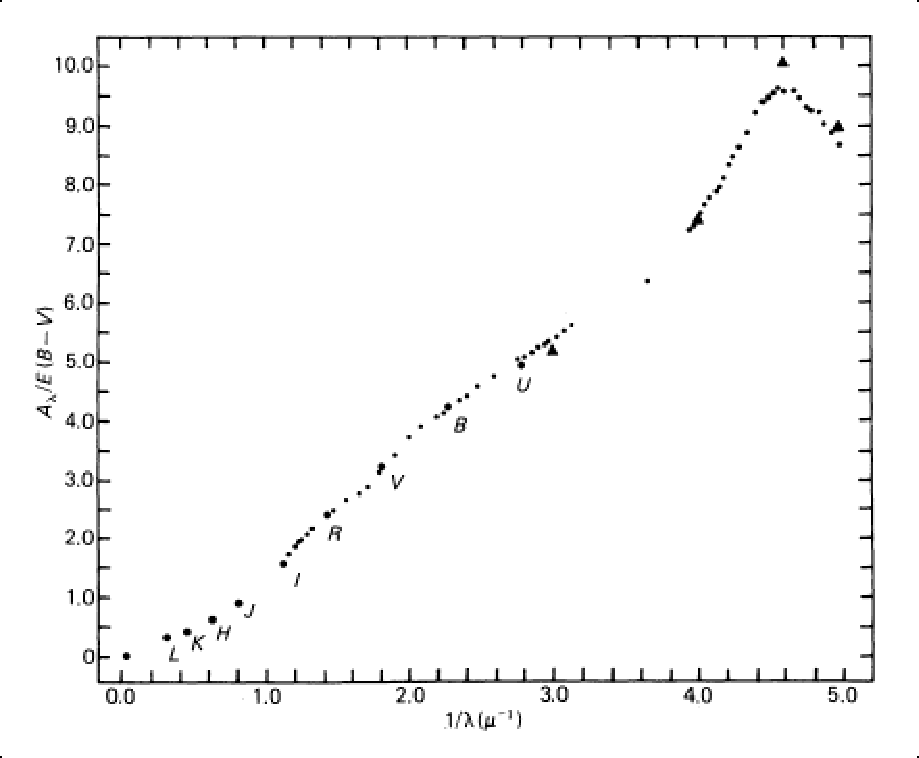
\includegraphics[width=0.5\textwidth]{interstellarreddeningreduite}
  \label{extinction}
  \caption{Variation de $A_V/E_{B-V}$ en fonction de $1/\lambda$}
\end{figure}

\begin{Answer}
  \begin{enumerate}
  \item Calcul de l'extinction
    $$
    E_{B-V} = (A_B- A_V) = (B-V )- (B-V)_0 = 2,25-(-0,25) = 2
    $$
    Le graphique donne $A_V = 3 E_{B-V}$, d'où:
    $$
    A_V =3 \times 2 = 6
    $$
  \item Le graphique donne $A_K = 0.5 \times E_{B-V}$, d'où:
    $$
    A_K = 0.5 \times 2 = 1
    $$
  \item L'extinction est beaucoup plus faible dans l'IR que dans le
    visible.
  \end{enumerate}
\end{Answer}

\section{Galaxies}

\subsection{Classification morphologique des galaxies}

\begin{Exercise}[Propriétés « physiques » de la classification]
  En vous servant du tableau sur les propriétés quantitatives de la
  séquence de Hubble, répondez aux questions suivantes :
  \begin{enumerate}
  \item Que peut-on dire sur la fraction de gaz dans les galaxies
    selon le type morphologique ?
  \item Que peut-on dire de la densité surfacique de masse, en
    supposant que toute la masse des galaxies est concentrée dans un
    disque mince ?
  \end{enumerate}
\end{Exercise}

\begin{Answer}
  \begin{enumerate}
  \item La fraction de masse de gaz est donnée par le rapport de la
    masse de gaz à la masse totale. Ce rapport augmente des S0 aux
    irrégulières.
  \item La densité surfacique de masse est $S = M/ \pi R^2$. Elle
    diminue des S0 aux irrégulières.
  \end{enumerate}

  Dans le tableau ci-dessous, les valeurs de
  $M_{\mathrm{gaz}}/M_{\mathrm{totale}}$ et de $S$ sont obtenues
  statistiquement sur un échantillon de plusieurs milliers de
  galaxies. Ce ne sont donc pas les valeurs obtenues par le calcul
  direct sur les médianes, mais le comportement reste le même.

  \begin{center}
    \begin{tabular}{|c|c|c|c|c|c|c|}
      \hline
      Propriétés & E,SO & S0a,Sa & Sab,Sb & Sbc,Sc & Scd,Sd & Sm,Im \\
      \hline
      $M_{\mathrm{totale}}$ ($10^{10}M_{\odot}$) & & 22.6 & 32.4 & 19.0 & 7.9 &
      1.6 \\
      \hline
      $M_{\mathrm{gaz}}$ ($H$ neutre en $10^{9}M_{\odot}$) & 1.24 & 5.62 &
      15.14 & 15.85 & 9.33 & 2.40\\
      \hline
      $M_{\mathrm{gaz}}/M_{\mathrm{totale}}$ & & 0.03 & 0.05 & 0.08 & 0.11 & 0.15 \\
      \hline
      diamètre (kpc) & 21.1 & 19.8 & 25.1 & 22.4 & 17.7 & 8.5  \\
      \hline
      S ($M_{\odot}/pc^2$) &  & 188.9 & 154.7 & 124.2 & 91.4 & 74.5 \\
      \hline
    \end{tabular}
  \end{center}
\end{Answer}


\begin{Exercise}[de Vaucouleurs et autres classifications]
  Donnez la classification simplifiée (E, S0, SA, SAB, SB) des
  galaxies données dans la partie cours correspondante dans spirale.

  Est-il toujours facile de classifier les galaxies réelles?
\end{Exercise}

\begin{Answer}
  \begin{center}
    \begin{tabular}{|c|c|c|c|}
      \hline
      % \textbf{N° objet} & \textbf{Nom} & \textbf{Réponse} &
      % textbf{Classification complète dite RC3}\\ \hline
      1  & NGC6070    & SA  & SA(s)cd  \\ \hline
      2  & NGC 7424   & SAB & SAB(rs)cd  \\ \hline
      3  & MESSIER 31 & SA  & SA(s)b  \\ \hline
      4  & MESSIER 33 & SA  & SA(s)cd  \\ \hline
      5  & MESSIER 87 & E0 ou E1 & E+0-1 pec* \\ \hline
      6  & NGC 2683   & SA  & SA(rs)b  \\ \hline
      7  & NGC 1300   & SB  & (R')SN(r'1)b  \\ \hline
      8  & NGC 1097   & SB  & (R'\_1:)SB(r'l)b  \\ \hline
      9  & NGC 4321   & SAB & SAB(s)bc \\ \hline
      10 & MESSIER 83 & SAB & SAB(s)c \\ \hline
    \end{tabular}
  \end{center}

  Galaxies lointaines sans noms (11). La classification demandée est
  SB. Ces objets sont considérés comme des galaxies barrées mais n'ont
  pas été précisément classifiées à cause du manque de résolution des
  images (HST Deep Field North).

  *pec: 'peculiar' à cause du jet provenant du noyau actif
\end{Answer}

\subsection{Constituants des galaxies}

\begin{Exercise}[Les étoiles]
  Si l'on considère une sphère de rayon 10 kpc peuplée par $10^{11}$
  étoiles dont le rayon est égal à celui du soleil, calculez la
  fraction de volume occupé par les étoiles.
\end{Exercise}

\begin{Answer}
  La fraction est de $10^{11}\times \left(\frac{0.7\times
      10^{6}}{10\times 3.08\times 10^{16}}\right)^{3}\approx 10^{-20}$
\end{Answer}


\begin{Exercise}[La matière noire]
  Donnez l'expression de l'accélération $a$ centrifuge en fonction de
  $V$, et $R$, la vitesse circulaire d'une étoile à une distance $R$
  du centre de la galaxie.  Écrire la loi de Newton pour cette
  étoile~: l'accélération $a$ en fonction de la masse $M$ incluse dans
  le rayon $R$.  En déduire la loi de décroissance de $V$ en fonction
  du rayon $R$ de l'étoile, en supposant que la masse $M$ reste
  constante (c'est-à-dire que toute la masse de la galaxie est
  comprise dans la sphère de rayon $R$).
\end{Exercise}

\begin{Answer}
  L'accélération centrifuge est donnée simplement par $a = V^2/R$.  La
  loi de Newton nous dit alors que l'accélération de l'étoile est
  proportionnelle à la masse $M$ avec $a = G M/R^2$, où $G$ est la
  constante universelle de la gravitation.  On en déduit alors
  facilement que $V^2/R = GM/R^2$ donc $V^2 \propto M/R$.

  Si $M$ reste constant avec $R$ qui croit, alors $V^2$ doit décroître
  comme $1/R$.
\end{Answer}

\subsection{Exemple de galaxie : la Voie Lactée }

\begin{Exercise}[Morphologie de notre galaxie]
  En examinant en détail l'image de notre galaxie prise par COBE/DIRBE
  (Fig.~\ref{cobe}) on distingue que le bulbe de la Voie Lactée n'est
  pas symétrique.
  \begin{enumerate}
  \item Examiner cette image et essayer de mesurer la hauteur du
    bulbe~; à droite, puis à gauche du centre de la Galaxie
  \item Donner une explication plausible de cette asymétrie, en se
    rappelant notre position très particulière par rapport au centre
    de notre galaxie, et en se rappelant des différentes composantes
    qui composent notre Galaxie.
  \end{enumerate}
\end{Exercise}

\begin{figure}[htp]
  \centering
  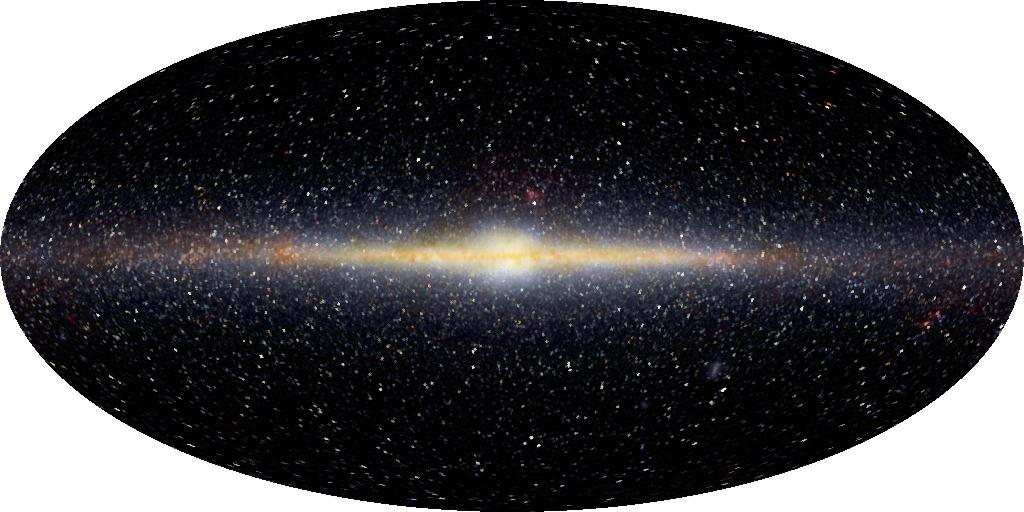
\includegraphics[width=0.8\textwidth]{milky2w}
  \label{cobe}
  \caption{Notre galaxie vue par COBE/DIRBE.}
\end{figure}

\begin{Answer}
  Le bulbe de la galaxie vue en infrarouge est effectivement
  asymétrique:
  \begin{enumerate}
  \item Le coté gauche a une épaisseur légèrement plus grande que le
    coté droit.
  \item Ça n'est pas un effet de populations stellaires, ou
    d'extinction due à la poussière, mais bien une épaisseur
    réellement plus grande d'un coté que de l'autre. Ce que l'on voit
    est en fait un effet de projection : c'est en fait la barre de la
    Galaxie que nous observons. Cette barre étant inclinée à 35 degrés
    environ par rapport à nous, le coté gauche étant proche de nous,
    le coté droit loin de nous (de l'autre coté du centre
    galactique). Une des extrémités de la barre est donc plus proche
    de nous, et par projection elle apparaît plus haute...
  \end{enumerate}
\end{Answer}

\begin{Exercise}[Le centre galactique]
  L'image ci-dessous (Fig.~\ref{centregalac}) montre l'orbite de
  l'étoile ayant la plus grande vitesse autour du centre galactique. À
  partir des données (période en années de 15.2 ans, et demi grand-axe
  de 0.119 arcsecondes) de cette orbite, retrouver l'estimation de la
  masse incluse dans ce rayon au centre de notre Galaxie en utilisant
  la troisième loi de Kepler. On rappelle que nous sommes à environ
  8.5~kpc du centre galactique et que G, la constante
  gravitationnelle, vaut $6,6742.10^{-11} m^3 kg^{-1} sec^{-2}$.  La
  masse visible étant estimée à environ 106 masses solaires, en
  déduire une estimation de la masse noire centrale (le fameux trou
  noir) de notre Galaxie.
\end{Exercise}

\begin{figure}[htp]
  \centering
  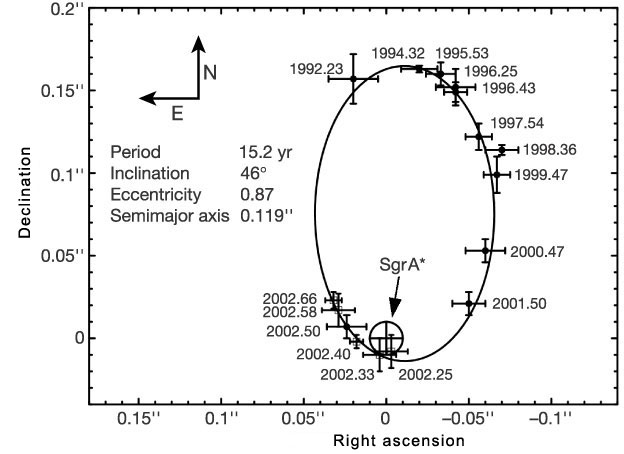
\includegraphics[width=0.5\textwidth]{nature01121-f2_2}
  \label{centregalac}
  \caption{Orbite de l'étoile S2 autour du centre galactique SgrA*
    (Schödel et al. 2002).}
\end{figure}

\begin{Answer}
  On rappelle que G, la constante gravitationnelle, vaut
  $6,6742.10^{-11} m^3kg^{-1}sec^{-2}$

  Nous allons d'abord transformer la taille du demi grand-axe
  d'arcseconde en mètres, et ensuite, la période en secondes:
  \begin{itemize}
  \item 1 arcseconde équivaut à $1/3600$~degrés, donc à $8.5~kpc$ ,
    cela revient à environ $0.041~pc$. Le demi grand axe est donné
    comme étant égal à $0.119$~arcseconde, donc cela équivaut à~:
    $$
    a = 0.119\times0.041 = 0.0048~pc = 0.0048\times 3.08 \times
    10^{16} = 1.5 \times 10^{14}~m
    $$

  \item la période $T$ est donnée de 15.2 ans donc~: $T=479347200~s$
  \end{itemize}

  Enfin la troisième loi de Kepler dit que le rapport $T^2/a^3$ est une
  constante k qui ne dépend que de la masse du système.

  Cette constante k est simplement donnée par : $4\pi^2/(GM)$ donc on
  peut écrire que:
  $$
  M = \frac{4\pi^2 a^3}{T^2 G}
  $$

  En application numérique cela donne (en kg, vérifiez bien que
  l'équation est homogène dans ses unités):
  $$
  M = \frac{ 4 \times \pi^2 \times (1,5 \times 10^{14})^3 } { (479 347
    200)^2 \times 6,6742 \times 10^{11} } = 8,7 \times 10^{36}~kg
  $$
  et ceci exprimé en masses solaires: $M \approx 4,4 \times
  10^6~M_{\odot}$
\end{Answer}

\subsection{Le groupe local}

\begin{Exercise}
  Compter le nombre de galaxies ayant un diamètre plus petit que 6
  kpc, et celles ayant un diamètre plus grand. Quelles sont les
  galaxies qui dominent en nombre ? Et en luminosité totale ?
  (Fig.~\ref{listgalac})
\end{Exercise}

\begin{figure}[htp]
  \centering
  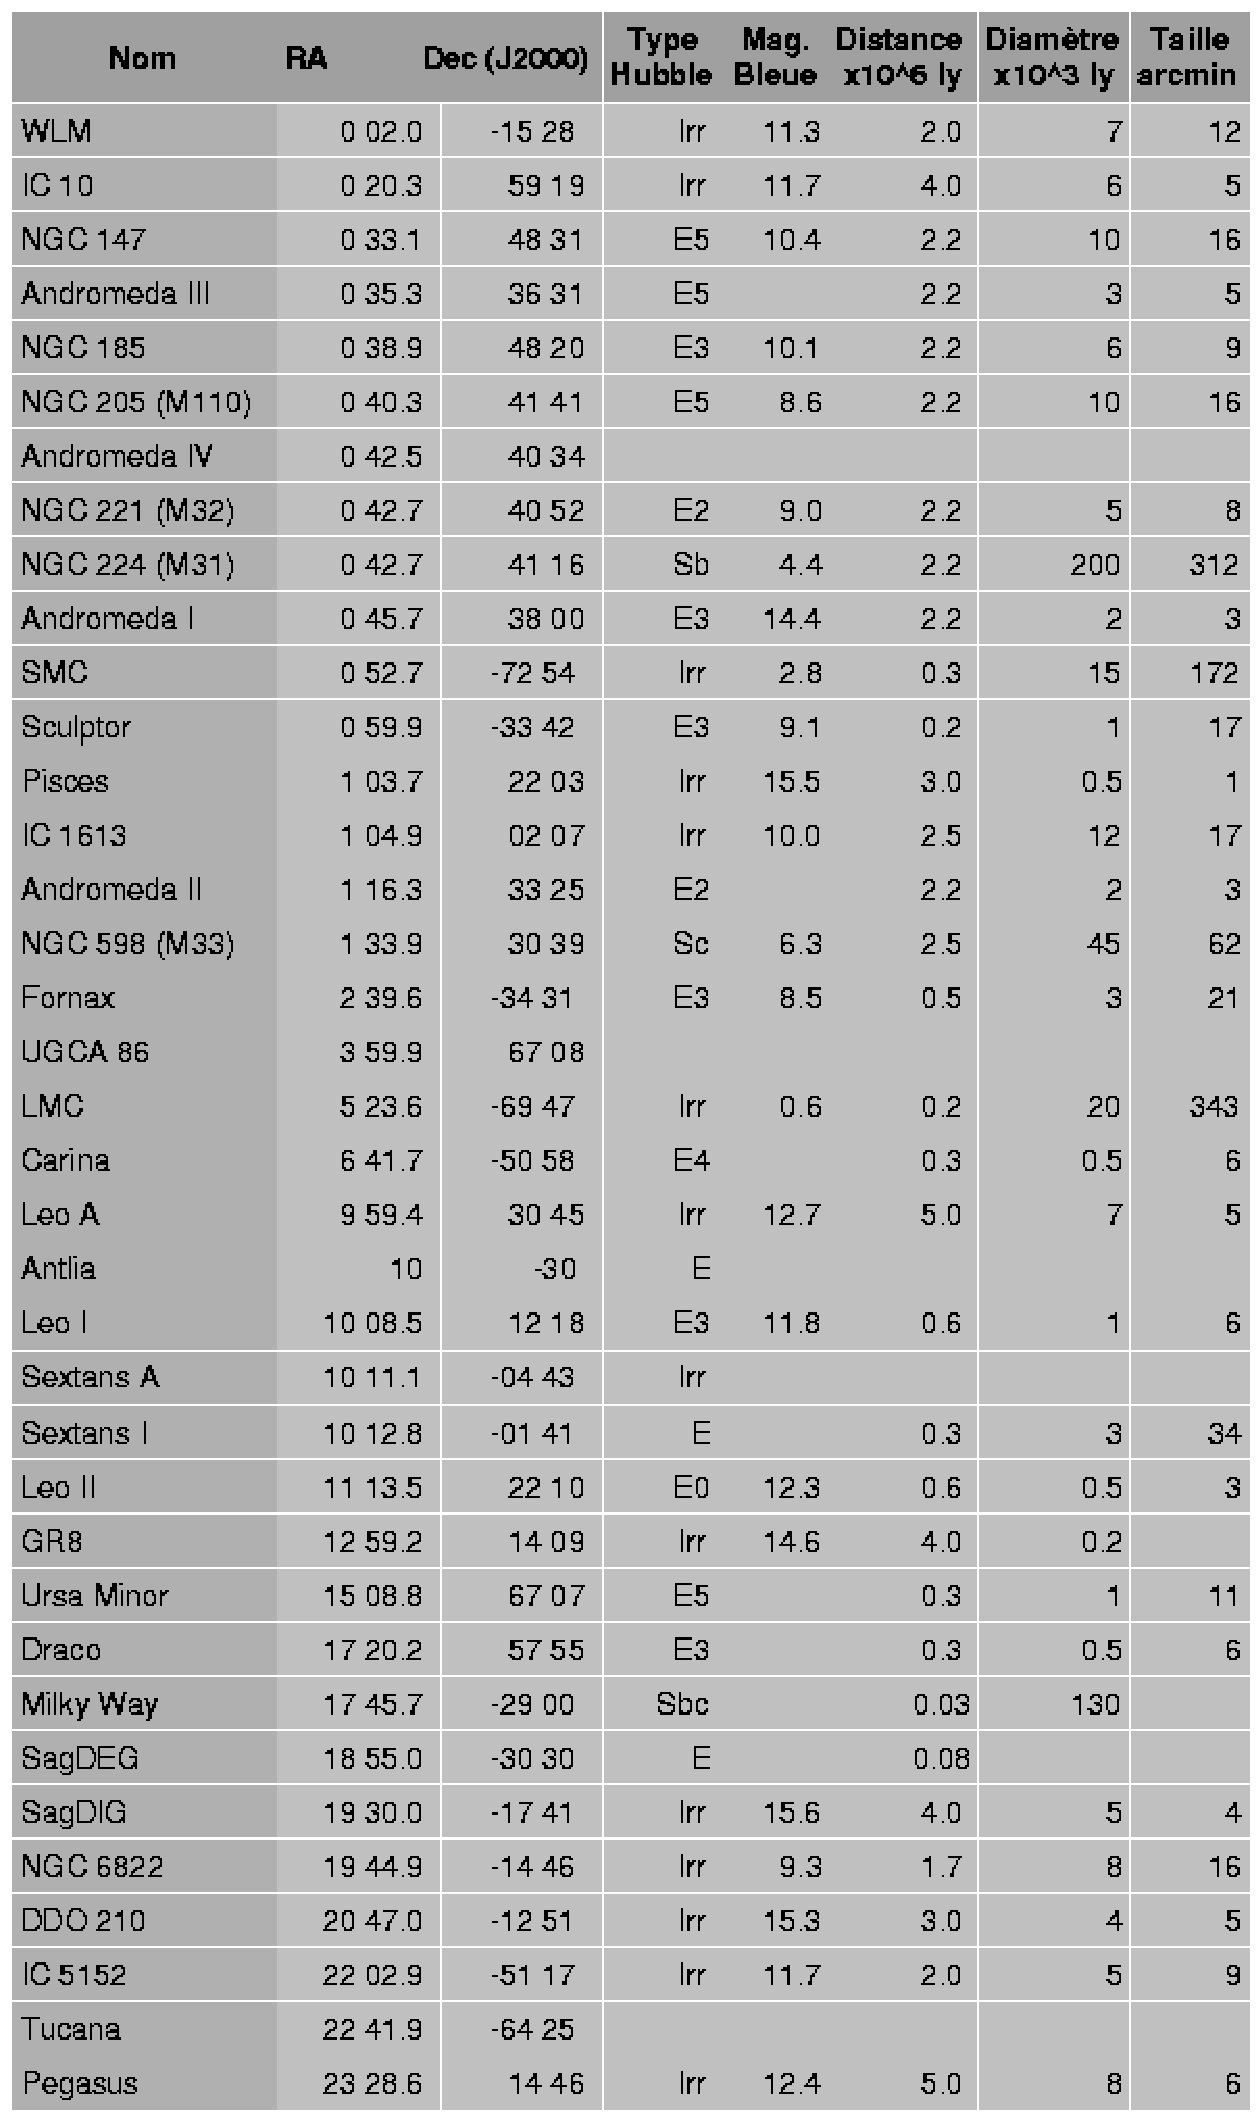
\includegraphics[height=\textheight]{listegalaxiegroupelocal}
  \label{listgalac}
  \caption{Liste des galaxies du Groupe Local, avec leurs noms, leurs
    positions sur le ciel, le type de Hubble, la distance, le diamètre
    en milliers d'années-lumière et en arcminutes sur le ciel.}
\end{figure}

\begin{Answer}
  Il y a 26 petites galaxies -- dites « naines » -- sur les 30
  galaxies dont on nous donne la taille, et seulement 2 galaxies avec
  un diamètre de plus de 30 kpc : M31 et la Voie Lactée). Ce sont donc
  les galaxies naines qui dominent en nombre, mais elles ne dominent
  pas en luminosité totale.
\end{Answer}

\subsection{Distribution des galaxies dans l'univers}

\begin{Exercise}[Fonction de luminosité]
  \begin{enumerate}
  \item Exprimer la loi de Schechter en magnitudes absolues.
  \item Quelle est la signification physique de la loi de Schechter?
  \end{enumerate}
\end{Exercise}

\begin{Answer}
  \begin{enumerate}
  \item En magnitude
    $$
    \Phi (M) = 0.4 \ln (10) \Phi ^{*}10^{0.4(\alpha +1)(M^{*}-M)}\exp
    \left( -10^{0.4(M^{*}-M)} \right)
    $$

  \item Cette fonction empirique montre bien la prédominance des
    galaxies de faible luminosité intrinsèque.
  \end{enumerate}
\end{Answer}

\subsubsection{Effets d'environnement, collisions et fusions}

\begin{Exercise}[Calcul de la fréquence des collisions dans un
  amas]
  On considère un amas de galaxies qui a les caractéristiques
  suivantes:
  \begin{itemize}
  \item il est supposé sphérique, de diamètre $D_{amas}$ en pc
  \item il contient $N_{galaxies}$ identiques et réparties
    uniformément dans l'amas
  \item les galaxies sont supposées animées d'une vitesse uniforme
    $v_{galaxies}$ en km/s
  \end{itemize}

  \begin{enumerate}
  \item Donner l'expression de la densité numérique de galaxies dans
    l'amas en $pc^{-3}$.

  \item On suppose maintenant que les galaxies ont un diamètre typique
    $D_{galaxies}$ (en pc). En modélisant les galaxies comme des
    sphères dures (boules de billard...) de diamètre $D_{galaxies}$,
    donner l'expression de la section efficace $S_{efficace}$ (en
    $pc^2$) lors d'une collision/interaction entre deux galaxies.

  \item Donner l'expression du nombre de collisions/interactions que
    subit une galaxie de l'amas pendant la durée $dt$ (en années). En
    déduire, pour une galaxie, le temps caractéristique de collision
    et le libre parcours moyen.

  \item En déduire le temps entre deux collisions/interactions dans
    l'amas.

  \item Calcul de la fréquence des collisions dans un amas:
    Considérons un amas de $N=850$ galaxies dont le diamètre est
    $D=7~Mpc$ et dont la dispersion des vitesses est $V =
    650~km/s$. Explicitez le calcul numérique du temps moyen entre
    deux collisions pour l'amas considéré.
  \end{enumerate}
\end{Exercise}

\begin{Answer}
  \begin{enumerate}
  \item Le volume de l'amas est
    $$
    V_{amas}=\frac{\pi}{6}D_{amas}^3
    $$
    et la densité numérique de galaxies est donc
    $$
    n_{galaxies}=\frac{N_{galaxies}}{V_{amas}}=
    \frac{6N_{galaxies}}{\pi D_{amas}^3}
    $$
    (en nombre de galaxies par $pc^3$ si le diamètre de l'amas est en
    pc)

  \item Deux galaxies entreront en collision/interaction lorsqu'elle
    passent à une distance < $D_{galaxies}$ l'une de l'autre. La
    section efficace de collision est donc $S_{efficace}=\pi
    D^2_{galaxies}$ en $pc^2$ si le diamètre des galaxies est exprimé
    en $pc$.

  \item Le volume «balayé» par une galaxie pendant le temps dt est le
    suivant:
    $$
    V = \frac{3.15\,10^7 \text{(s par année)}}{%
      3.09\,10^{13} \text{(km par pc)}}
    \times v_{galaxies} \times S_{efficace} \times dt
    $$
    Le nombre de collisions pendant ce temps $dt$ est donc
    $N_{collision} = n_{galaxie}V$. Le temps caractéristique de
    collision/interaction $t_{collision}$ correspond à $dt$ tel que
    $N_{collisions} = 1$. Le libre parcours moyen est $l =
    v_{galaxies} \times t_{collision}$.
    $$
    \tau_{collision} =
    \frac{3.09 \times 10^{13}}{6 \times 3.15 \times 10^7}
    \frac{D^3_{amas}}{D^2_{galaxies} \times v_{galaxies} \times N_{galaxies}}
    $$

  \item Le temps caractéristique de collision/interaction dans l'amas
    est $t_{collision}^{amas} = \tau_{collision}/N_{galaxies}$ (on
    considère ici l'amas entier et non plus une galaxie unique).
  \end{enumerate}

\end{Answer}



\subsection{Équilibre gravitationnel}

\begin{Exercise}[Théorème du Viriel scalaire]
  Le théorème du Viriel peut aussi s'écrire :
  $$
  \frac{2K}{U}=-1
  $$
  Imaginez que vous vouliez construire un système stellaire, en
  donnant à $N$ étoiles leurs positions et leurs vitesses, et où vous
  auriez:
  $$
  \frac{2K}{U}>-1
  $$
  \begin{enumerate}
  \item Comment feriez-vous ? (donner un exemple)
  \item Comment le système évoluerait-il ?
  \end{enumerate}
\end{Exercise}

\begin{Answer}
  \begin{enumerate}
  \item Il suffit de donner une position quelconque aux étoiles mais
    en leur donnant à toute une vitesse nulle. On aurait alors $K=0$,
    et ainsi on aurait bien la condition remplie!

  \item Si cette condition est remplie, c'est que l'énergie cinétique
    est trop faible par rapport à l'énergie potentielle (en valeur
    absolue). Il manque aux étoiles de la vitesse pour que le système
    reste à l'équilibre, et il va donc se réarranger, avec un rayon
    plus petit.
  \end{enumerate}
\end{Answer}

\begin{Exercise}[Application du théorème du Viriel]
  On va maintenant utiliser le théorème du Viriel pour remplir le
  tableau ci-dessous, donnant les rayons, masses et vitesse
  caractéristiques de différents système stellaires.  Veuillez
  compléter ce tableau.  (On prendra $G$ en fonction d'unités
  astronomiques pratiques, ainsi $G=0.004301$
  pc.km$^{2}$.s$^{-2}$.M$_{\odot}^{-1}$)

  \begin{center}
    \begin{tabular}{|c|c|c|c|}
      \hline
      Système & R (pc) & V (km/s) & M ($M_{\odot}$) \\ \hline
      Amas globulaire & 10 & 10 &  \\ \hline
      Galaxie & 50~000 & 200 & \\ \hline
      Amas de galaxies & 1~000~000  & 1000  &  \\ \hline
    \end{tabular}
  \end{center}
\end{Exercise}

\begin{Answer}
  \begin{center}
    \begin{tabular}{|c|c|c|c|}
      \hline
      Système & R (pc) & V (km/s) & M ($M_{\odot}$) \\ \hline
      Amas globulaire & 10 & 10 & $1,4\times 10^6$ \\ \hline
      Galaxie & 50~000 & 200 & $2,3\times 10^{11}$ \\ \hline
      Amas de galaxies & 1~000~000  & 1000  &  $1,4\times 10^{15}$ \\ \hline
    \end{tabular}
  \end{center}
\end{Answer}

\begin{Exercise}[Temps cinématique]
  On va maintenant calculer le temps cinématique $t_c$ pour différents
  systèmes stellaires. Veuillez compléter le tableau ci-dessous.  (Une
  fois de plus, on prendra $G$ en fonction d'unités astronomiques
  pratiques, ainsi $G=0.004301$ pc.km$^{2}$.s$^{-2}$.M$_{\odot}^{-1}$)
  \begin{center}
    \begin{tabular}{|c|c|c|c|}
      \hline
      Système & R (pc) & M ($M_{\odot}$) & $t_c$ (ans) \\ \hline
      Amas ouvert & 1 & 500 &  \\ \hline
      Amas globulaire & 10 & $10^5$ &  \\ \hline
      Galaxie & 50~000 & $10^{12}$ & \\ \hline
    \end{tabular}
  \end{center}
  Que remarquez-vous sur ces temps cinématiques pour les différents
  systèmes ?
\end{Exercise}

\begin{Answer}
  \begin{center}
    \begin{tabular}{|c|c|c|c|}
      \hline
      Système & R (pc) & M ($M_{\odot}$) & $t_c$ (ans) \\ \hline
      Amas ouvert & 1 & 500 & $10^6$ \\ \hline
      Amas globulaire & 10 & $10^5$ & $2\times 10^6$ \\ \hline
      Galaxie & 50~000 & $10^{12}$ & $2\times 10^8$ \\ \hline
    \end{tabular}
  \end{center}

  Les temps cinématiques pour un amas ouvert et un amas globulaire ne
  sont pas vraiment différents malgré leurs tailles respectives très
  différentes.  De même entre une galaxie et un amas globulaire: il ne
  faut qu'environ 100 plus de temps à une étoile avec une vitesse
  typique pour traverser une grosse galaxies qu'un amas globulaire
  (bien sur les vitesses caractéristiques ne sont pas les mêmes pour
  ces 2 systèmes).
\end{Answer}

% ===============================================================================

\chapter{Vie des structures - Cosmologies}

\section{Espace et temps absolus}

\begin{Exercise}[La faiblesse de la force de gravitation]
  Marcel et Naomi ressentent l'un pour l'autre une certaine attirance;
  quelle part en revient tout bêtement à la force de gravitation
  universelle, lorsque leurs centres de gravité respectifs sont
  distants de 1 mètre ?  Quelle masse, au même point de la Terre,
  présente un poids égal à cette force ?  Marcel pèse, à Lyon, 700 N,
  et Naomi 580 N.  Le rayon de la Terre à Lyon sera supposé égal à
  6365~km.  La constante de la gravitation et la masse de la Terre
  sont données dans les annexes du cours...
\end{Exercise}

\begin{Answer}
  Il s'agit, simplement, d'appliquer la formule de Newton deux fois
  pour trouver les masses respectives de Marcel et Naomi, puis une
  troisième fois pour calculer l'attraction qui s'exerce entre eux, en
  prenant garde aux unités.
  $$
  F = G \frac{m_1 m_2}{d^2}
  $$

  On retrouve d'abord les valeurs des constantes : $G = 6,672 \times
  10^{-11}$, $M_{\oplus} = 5,976 \times 10^{24}~kg$, et $R = 6365~km$
  qui est donné dans l'énoncé.

  On écrit donc:
  $$
  P_{\mathrm{Marcel}} = G \frac{M_{\mathrm{Marcel}}M_{\oplus}}{R^2}
  $$
  soit encore:
  $$
  M_{\mathrm{Marcel}} = \frac{P_{\mathrm{Marcel}}R^2}{G M_{\oplus}}
  $$
  et donc
  $$
  M_{\mathrm{Marcel}} = \frac{ 6370000^2 \times 700 }{ 6,672 \times
    10^{-11} \times 5,976 \times 10^{24} } = 71,23~kg
  $$
  Cette valeur s'obtiendrait aussi en utilisant la formule $P =
  M_{\mathrm{Marcel}}\times g$, où $g$ est l'accélération de la
  pesanteur à Lyon. Mais l'énoncé ne précise pas la valeur de $g$ à
  Lyon...

  Pour Naomi, on peut utiliser le fait que
  $M_{\mathrm{Naomi}}/M_{\mathrm{Marcel}} =
  P_{\mathrm{Naomi}}/P_{\mathrm{Marcel}}$, puisque les deux personnes
  sont soumises au même champ de gravité. Et donc:
  $$
  M_{\mathrm{Naomi}} = M_{\mathrm{Marcel}}
  \frac{P_{\mathrm{Naomi}}}{P_{\mathrm{Marcel}}} = 71,23 \times
  \frac{58}{70} = 59,02~kg
  $$
  D'où $F_{\mathrm{Naomi}-\mathrm{Marcel}} = ( 6,672 10^{-11} \times
  71,23 \times 59,02 ) / 1 = 2,8 10^{-7}~N$.

  La masse qui présenterait un poids égal à cette valeur en cet
  endroit serait de : $M = ( 63700002 \times 2,8 10^{-7} ) / ( 6,672
  10^{-11} \times 5,976 10^{24} ) = 2,85 10^{-8} kg = 28,5~\mu g$.

  Elle peut également se calculer, d'après une remarque déjà faite,
  par $M = 71,23 \times 2,8 10^{-7} / 700$. L'attraction
  gravitationnelle est une force \emph{très faible}, c'est même la
  plus faible des quatre forces fondamentales de l'univers...
\end{Answer}

\subsection{Problèmes de l'univers de Newton}

\begin{Exercise}[L'instabilité gravitationnelle]
  Pourquoi Newton pense-t-il que ces trois hypothèses supplémentaires
  permettraient, chacune, de « sauver » l'univers de la catastrophe
  gravitationnelle?
\end{Exercise}

\begin{Answer}
  \begin{itemize}
  \item Si l'univers est infini, tout point est entouré d'une
    distribution de matière à symétrie sphérique, et restera donc
    immobile.
  \item Si l'univers est en expansion, et bien, tant qu'il l'est,
    c'est qu'il n'est pas en train de se contracter !
  \item Si l'univers est très jeune, il n'a pas encore eu le temps de
    démarrer sa contraction gravitationnelle de façon sensible, et
    voilà ...
  \end{itemize}
\end{Answer}

\begin{Exercise}[Le paradoxe d'Olbers]
  En quoi le fait que l'univers soit jeune et en expansion peut-il
  permettre d'expliquer la noirceur du ciel nocturne ?
\end{Exercise}

\begin{Answer}
  \begin{itemize}
  \item Si l'univers est jeune, du fait de la vitesse finie de
    propagation de la lumière, celle qui provient des objets très
    lointains n'a pas eu le temps de nous parvenir.
  \item Si l'univers est en expansion, la lumière qui nous parvient
    des objets très lointains a été affaiblie par cette expansion
    (ceci sera traité plus loin dans le cours), au point de ne pas
    être détectable.
  \end{itemize}
\end{Answer}

\section{La rupture relativiste}

\subsection{Vitesse de la lumière}

\begin{Exercise}[La première mesure de $c$]
  Si Roemer a fait le calcul (ce que l'on ignore, mais cela semble
  assez probable), et en supposant qu'il utilisait la même valeur de
  la distance Terre-Soleil que les astronomes d'aujourd'hui, quelle
  valeur de $c$ a-t-il obtenue?
\end{Exercise}

\begin{Answer}
  Si la lumière met $8+8 = 16$ minutes pour traverser l'orbite de la
  Terre, c'est à dire pour franchir une distance de $2~U.A$., sa
  vitesse est $c = 2 \times 1,49598 \times 10^{11} / ( 16 \times 60 )
  = 3,11 \times 10^8~m~s^{-1}$. Ceci suppose que la valeur de
  l'U.A. admise alors était la même qu'aujourd'hui, ce qui n'est
  certainement pas exact : en 1675, on n'avait pas encore très bien
  mesuré la distance de la Terre au Soleil ... La valeur de deux fois
  huit minutes est elle-même approximative. Roemer aurait plutôt
  trouvé $2 \times 10^8~m~s-1$, dit-on. La première détermination
  sérieuse de l'Unité Astronomique est due à Cassini et Richer, en
  1671. Il faudra attendre le XXe siècle et les méthodes d'écho radar
  pour disposer de mesures très précises de cette valeur.
\end{Answer}

\subsection{Relativité générale}

\subsubsection{Einstein dans l'ascenseur}

\begin{Exercise}[L'équivalence gravité/accélération]
  On dit que, pour la Relativité Générale, gravitation et accélération
  sont équivalentes, mais que cette équivalence n'est que
  locale. C'est à dire qu'aucune expérience de physique ne permet de
  distinguer les effets de l'une de ceux de l'autre, mais seulement
  tant qu'on se limite à un très petit domaine spatial. En gros, c'est
  à peu près vrai dans un dé à coudre, cela ne l'est plus vraiment
  dans un stade de foot...

  En reprenant l'exemple simple de l'ascenseur d'Einstein, pouvez-vous
  montrer qu'en effet il est facile de distinguer pesanteur et
  accélération par la fusée si on abandonne la localité. Il suffit de
  modifier l'ascenseur...
\end{Exercise}

\begin{Answer}
  À grande échelle, le champ de gravité qui environne un corps massif
  reste en général tout à fait discernable d'une accélération
  constante.  Par exemple, dans l'image de l'ascenseur utilisée dans
  le cours, il ne faut pas que la cabine soit trop étendue. Sinon, le
  parallélisme ou le non-parallélisme des actions sur des masses très
  éloignées l'une de l'autre trahirait la « vraie » nature du champ.
  La cabine de gauche, supposée à grande distance de la planète, et
  accélérée vers le haut (flèche bleue), produit des actions
  parallèles (flèches rouges) sur les deux masses-test. La cabine de
  droite, immobile dans le champ de gravitation de la Terre, montre
  des actions convergentes vers le centre de la Terre (flèches
  vertes). Rusés comme ils le sont parfois, les physiciens de
  l'ascenseur finiraient par s'en apercevoir... (Fig.~\ref{grav})

  \begin{figure}[htp]
    \centering
    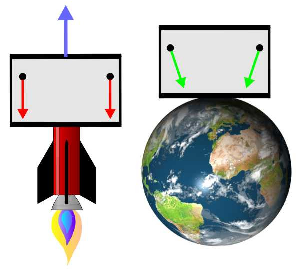
\includegraphics[width=0.4\textwidth]{grav}
    \caption{}
    \label{grav}
  \end{figure}
\end{Answer}

\subsection{Les tests}

\begin{Exercise}[Le décalage gravitationnel vers le rouge]
  Une lampe spectrale émettant la raie Hydrogène Alpha (de longueur
  d'onde en laboratoire 656,3 nm) est utilisée pour communiquer à
  partir d'une capsule en orbite serrée autour d'une étoile à
  neutrons. Le rayon de l'orbite est de 1000 km, la masse de l'étoile
  de 1,5 masses solaires.  À quelle longueur d'onde le vaisseau qui a
  lancé la capsule, et se tient prudemment à grande distance, doit-il
  rechercher les signaux?
\end{Exercise}

\begin{Answer}
  Le décalage gravitationnel subi à la distance r d'un corps de masse
  M s'écrit:
  $$
  z = \frac{GM}{c^2r}
  $$
  Et donc:
  $$
  z = \frac{ 6,672 \times 10^{-11} \times 1,5 \times 1,989 \times
    10^{30} }{ 2997924582 \times 10^6 } = 2,215 \times 10^{-3}
  $$
  Mais:
  $$
  z = \frac{ \delta \lambda } { \lambda_0 }
  $$
  Et donc:
  $$
  \lambda = \lambda_0 + \delta \lambda = (1+z)\lambda_0
  $$
  D'où le $\lambda$ cherché: $\lambda = 1,00221 \times 656,3 =
  657,75~nm$.
\end{Answer}

\section{Le big bang}

\subsection{Expansion de l'univers...}

\begin{Exercise}[...limitée par $c$?]
  Plus une galaxie est éloignée de notre Voie Lactée, plus les
  astronomes lui trouvent une vitesse d'éloignement élevée. C'est
  l'expansion de l'univers. Mais, quand la distance croît sans cesse,
  elle atteint un moment une valeur $d_c$ telle que :
  $$
  V = H_0 d_c > c
  $$
  Invraisemblable, n'est-ce pas ?
\end{Exercise}

\begin{Answer}
  Il est interdit par la Relativité Générale de mesurer une vitesse
  égale ou supérieure à $c$ pour un objet de masse non nulle, comme
  une galaxie. Alors ?

  Alors, cela ne pose aucun problème pour l'expansion de l'univers, où
  les objets (les galaxies...) sont immobiles dans un espace dont la
  géométrie s'étire. Les galaxies très lointaines voient effectivement
  leur vitesse apparente atteindre celle de la lumière, et
  disparaissent alors de l'univers observable. Ceci n'enlève rien au
  fait qu'elles continuent à s'éloigner de nous à des vitesses
  supérieures à $c$.

  Signalons que nos moyens d'observation actuels sont loin de nous
  permettre d'observer les objets qui flirtent avec cette limite...
\end{Answer}

\begin{Exercise}[...la même partout?]
  La radiogalaxie 3C 171 (nommée ainsi parce qu'elle occupe la 171e
  position dans le troisième catalogue de radiources établi par
  l'observatoire de Cambridge...) est relativement lointaine;
  entraînée par l'expansion de l'univers, elle présente une vitesse de
  fuite de 63000 km par seconde.

  Montrer que malgré cela, l'astronome Xhbrr'ffttk, qui a là-bas
  découvert l'expansion de l'univers, comme Hubble l'a fait pour nous,
  a lui aussi trouvé une loi qui s'écrit :
  $$
  V_0 = X_0 d_{0^{'}} \quad\text{avec}\quad X_0 = H_0
  $$
  $V_0$ étant la vitesse mesurée à partir de 3C171 pour une galaxie
  lointaine située à la distance $d_0$ de 3C171, et $X_0$ étant bien
  entendu la constante de Xhbrr'ffttk.

  Ainsi, d'une planète de 3C171, comme de la Terre, on observe la même
  expansion universelle, avec la même géométrie, et le même taux...
\end{Exercise}

\begin{Answer}
  Désignons par $V_T$ et $d_T$ les vitesses et distances mesurées à
  partir de la Terre, $V_{3C}$ et $d_{3C}$ celles mesurées à partir de
  3C171.  La vitesse de récession de 3C171 mesurée de la Terre est
  donc $v_T(3C171) = 63000~km/s$.

  Considérons une autre galaxie, G, observée à la fois de la Terre et
  de 3C171. On peut écrire :
  \begin{eqnarray*}
    \vec{V}_{3C}(G) &=& \vec{V}_{3G}(T) + \vec{V}_{T}(G) \\
    &=& -\vec{V}_{T}(3C171) + \vec{V}_{T}(G) \\
    &=& -H_0\vec{d}_{T}(3C171) + H_0\vec{d}_{T}(G) \\
    &=& H_0 \left[ \vec{d}_{T}(G) - \vec{d}_{T}(3C171) \right ] \\
    &=& H_0 \vec{d}_{3C}(G)
  \end{eqnarray*}
  et donc, à partir de 3C171 comme de la Terre, toute les galaxie
  observée semble s'enfuir avec une vitesse proportionnelle à sa
  distance, et le facteur de proportionnalité (la constante de
  Xhbrr'ffttk) est universel : $X_0=H_0$... (Fig.~\ref{H0})

  \begin{figure}[htp]
    \centering
    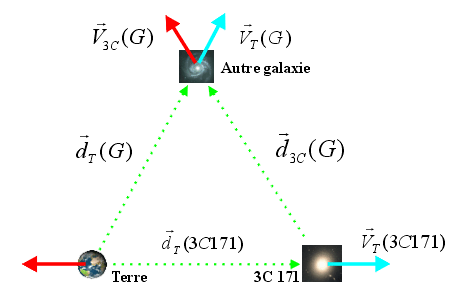
\includegraphics[width=0.4\textwidth]{351922_281}
    \caption{}
    \label{H0}
  \end{figure}
\end{Answer}

\begin{Exercise}[Le facteur d'expansion de l'espace]
  Donner $H_0$ en kilomètres par seconde et par mégaparsec est
  pratique pour les astronomes, mais ne parle guère à l'imagination.
  Passons donc dans des unités plus gouleyantes : si l'on suppose que
  $H_0 = 65 km s^{-1} Mpc^{-1}$, quelle est la valeur de
  l'accroissement annuel d'un kilomètre ? Des mètres ? Des millimètres
  ? Encore moins ?  Beaucoup plus?
\end{Exercise}

\begin{Answer}
  Un mégaparsec (Mpc) vaut $10^6$ parsecs, soit $3.26 10^6$
  années-lumière, soit $3,08 10^{19}~km$... Ceci nous montre que
  $65~km~s^{-1}~Mpc^{-1}$ équivalent à $2,10
  10^{18}~km~s^{-1}~km^{-1}$, ou encore $6,65
  10^{-11}~km~an^{-1}~km^{-1}$. Ce qui signifie que chaque kilomètre
  de l'espace, loin de toute galaxie, s'étire chaque année de $6,65
  10^{-11}~km$, soit environ 67 nanomètres! C'est infiniment dérisoire
  sur un kilomètre, mais sur les distances cosmiques l'effet est
  cumulatif, et cela donne des vitesses qui peuvent être très
  importantes, facilement de l'ordre de celle de la lumière...
\end{Answer}

\subsection{Facteur d'échelle}

\begin{Exercise}[Redshift et facteur d'échelle]
  La radiogalaxie 4C41.17 montre une raie spectrale intense à
  583,2~nm.  Cette raie est identifiée comme la raie Lyman alpha de
  l'hydrogène. En laboratoire, sur la Terre, la longueur d'onde de
  cette raie est de 121,5~nm. Quel était le facteur d'échelle de
  l'univers à l'époque où les atomes d'hydrogène de 4C41.17 émettaient
  cette raie ?
\end{Exercise}

\begin{Answer}
  Il suffit de se souvenir de la relation:
  $$
  1 + z = \frac{\lambda_\text{observé}}{\lambda_\text{émis}} =
  \frac{R_0}{R_\text{émission}}
  $$
  pour trouver $R_{em} = R_0 \times \lambda_{em}/\lambda_0 =
  \lambda_{em}/\lambda_{0}$. Et donc $R_{em} = 121,5/583,2 = 0,208$.
  À l'époque où 4C41.17 émettait la lumière qui nous parvient
  aujourd'hui, l'univers était cinq fois moins « étiré »
  qu'aujourd'hui... Remarquez bien qu'on évite de dire qu'il était
  moins « étendu » : cette expression sous-entendrait des choses sur
  la « taille globale » de l'univers, ce que tout cosmologiste
  raisonnable évite soigneusement de faire, vu son ignorance.
\end{Answer}

\begin{Exercise}[Facteur d'échelle et époque]
  À quelle époque $t_{em}$ la radiogalaxie 4C41.17 de l'exercice
  précédent a-t-elle émis la lumière que nous recevons aujourd'hui à
  $t_0$? On prendra $t_0 = 13.5$ milliards d'années.
\end{Exercise}

\begin{Answer}
  Il suffit de se souvenir de la relation liant le facteur d'échelle
  et le temps cosmologique :
  $$
  R(t)/R_{0} = \left(\frac{t}{t_0}\right)^{2/3}
  $$
  pour trouver $t_{em} = t_0 \times
  \left(R(t_{em})/R_{0}\right)^{3/2}$, et donc $t_{em} = 13,5 \times
  (0,208)^{1,5} = 1,3$~Gan.  4C41.17 émettait la lumière qui nous
  parvient aujourd'hui alors l'univers était âgé d'environ 1,3
  milliards d'années. Environ, car l'équation de départ n'est qu'une
  approximation.
\end{Answer}

\begin{Exercise}[Redshift cosmologique]
  Quel est le redshift de la radiogalaxie 4C41.17 citée dans
  l'exercice précédent?
\end{Exercise}

\begin{Answer}
  On reprend la relation:
  $$
  1 + z = \frac{\lambda_\text{observé}}{\lambda_\text{émis}} =
  \frac{R_0}{R_\text{émission}}
  $$
  pour trouver $1 + z = 1 / 0,208 = 4,807$, et donc $z = 3,807$.
\end{Answer}

\subsection{Film des débuts}

\begin{Exercise}[Nucléosynthèse primordiale ou non?]
  Les éléments légers $\mathrm{H}$, ${}^{2}\mathrm{H}$,
  ${}^{3}\mathrm{H}$, ${}^{4}\mathrm{He}$, ${}^{7}\mathrm{Li}$ sont
  nés avec le Big Bang. Mais d'où proviennent tous les autres éléments
  « lourds », ceux qui entrent dans la composition des objets du
  quotidien ?
\end{Exercise}

\begin{Answer}
  Les chapitres traitant des modèles stellaires et de l'évolution
  stellaire nous fournissent la réponse :
  \begin{itemize}
  \item Jusqu'au ${}^{56}\mathrm{Fe}$, les noyaux sont produits par
    les étoiles.  La source d'énergie de celles-ci est d'origine
    thermonucléaire, et elles sont des usines à fabriquer, par fusion,
    des noyaux lourds à partir de noyaux plus légers.
  \item Au-delà, seules les explosions de supernovae atteignent des
    températures suffisantes (plusieurs $10^9~K$) pour pouvoir
    synthétiser les noyaux très lourds, jusqu'aux éléments
    transuraniens.
  \item Quelques noyaux particuliers (${}^{6}\mathrm{Li}$,
    ${}^{9}\mathrm{Be}$, ${}^{10}\mathrm{B}$) sont sans doute formés
    lors des collisions des rayons cosmiques avec la matière
    interstellaire.
  \end{itemize}
\end{Answer}


\section{Questions diverses}

\subsection{Âge de l'univers}

\begin{Exercise}[Calcul du temps de Hubble]
  La valeur la plus probable, aujourd'hui, de la constante de Hubble
  est $H_0 = 65\;\u{km s^{-1} Mpc^{-1}}$ Quelle conclusion
  pouvez-vous en tirer sur l'âge réel de l'univers?
\end{Exercise}

\begin{Answer}
  Le temps de Hubble est défini par: $1/t_{H0} = H_0 =
  65~\u{km~s^{-1}~Mpc^{-1}}$. Il reste simplement à convertir les
  Mpc (megaparsecs) en kilomètres, et il vient : $1/t_{H0} =
  65~\u{km~s^{-1}} [3,26 10^{19}~\u{km}]^{-1} = 20 \times
  10^{-19}$~s, d'où $t = 5 \times 10^{17}~s = 16 \times
  10^9$~années. On peut donc penser que l'univers est âgé de moins de
  16~milliards d'années.
\end{Answer}

\begin{Exercise}[Age de l'univers et temps de Hubble]
  En partant de la définition de $H_0$ et de la relation trouvée dans
  la section précédente entre le facteur d'échelle $R$ et l'âge $t$ de
  l'univers dans le cas de la densité critique, trouver la relation
  entre $H$ et $t$.
\end{Exercise}

\begin{Answer}
  Par définition:
  $$
  v = H_0.d \quad\text{donc}\quad
  H_0 = \frac{v}{d} = \frac{\d d}{\d t} \frac{1}{d} =
  \frac{\d\left(\epsilon R \right)}{\d t}\frac{1}{\epsilon R}
  \hfill
  $$
  car toute distance, à un instant t, s'écrit:
  $$
  d = \epsilon R(t)
  $$
  où $\epsilon$ est une constante; Et donc:
  \begin{eqnarray*}
    H_0 &=& \frac{1}{R}\frac{\d R}{\d t} \\
    &=& \left ( \frac{t}{t_0} \right )^{-2/3} \times
    \frac{\d\left( \frac{t}{t_0} \right )^{2/3}}{\d t} \\
    &=& \left ( \frac{t}{t_0} \right )^{-2/3} \times
    \left( \frac{t}{t_0} \right)^{-1/3} \frac{2}{3} \frac{1}{t_0} \\
    &=& \left( \frac{t}{t_0} \right)^{-1} \times \frac{2}{3t_0} \\
    &=& \frac{2}{3t}
  \end{eqnarray*}
  Dans le cas critique (univers marginalement ouvert), l'âge de
  l'univers est égal aux deux-tiers du temps de Hubble.
\end{Answer}

\subsection{Distance de l'horizon}

\begin{Exercise}[{Temps de vol, distance, et expansion...}]
  Il y a dix milliards d'années, ce photon que nous recevons
  aujourd'hui a quitté une lointaine galaxie.
  \begin{enumerate}
  \item Cette galaxie se trouvait-elle à dix milliards
    d'années-lumière de nous au moment de l'émission ?
  \item Cette galaxie se trouve-t-elle aujourd'hui à dix milliards
    d'années-lumière de nous ?
  \end{enumerate}
\end{Exercise}

\begin{Answer}
  \begin{itemize}
  \item Le photon a voyagé pendant dix milliards d'années en luttant
    contre l'expansion de l'espace qui contrariait son mouvement; tout
    se passe comme s'il avait parcouru à la vitesse $c$ une distance
    supérieure à celle qui séparait la galaxie de nous au moment de
    l'émission.  Au moment de l'émission, la galaxie était donc à
    moins de dix milliards d'années-lumière de nous.
  \item Depuis que le photon a quitté la galaxie, celle-ci, entraînée
    par l'expansion, a continué à s'éloigner de nous. Le photon a bien
    parcouru (de son point de vue, en admettant qu'il en ait un) dix
    milliards d'années-lumière, puisque sa vitesse par rapport à
    l'espace est à tout instant égale à $c$, mais la galaxie a
    continué sa route pendant tout ce temps, et se trouve aujourd'hui
    à plus de dix milliards d'années-lumière de nous...
  \end{itemize}
\end{Answer}


% ==============================================================================

\chapter{Retour sur Terre - Nos repères dans le ciel}

\section{Se positionner dans le ciel}

\begin{Exercise}[Repérage]
  \begin{enumerate}
  \item Quelles sont les coordonnées horizontales des quatre points
    cardinaux?

  \item Peut-on définir les coordonnées horizontales pour un
    observateur installé au pôle Nord géographique ou au pôle Sud?

  \item Pour quelles valeurs de la hauteur et de la distance zénithale
    un astre est-il visible, c'est-à-dire au dessus de l'horizon?
  \end{enumerate}
\end{Exercise}

\begin{Answer}
  \begin{enumerate}
  \item Les points cardinaux étant par définition sur l'horizon, leurs
    hauteurs sont nulles. Les directions Est-Ouest et Nord-Sud étant
    orthogonales, on a à partir de l'origine la direction Sud
    (Fig.~\ref{position}):
    \begin{center}
      \begin{tabular}{|c|c|c|}
        \hline
        Points cardinaux & Azimut (degrés) & hauteur (degrés) \\ \hline
        Nord & 180 & 0 \\ \hline
        Est & 270 & 0 \\ \hline
        Sud & 0 & 0 \\ \hline
        Ouest & 90 & 0 \\ \hline
      \end{tabular}
    \end{center}
    Remarque: L'azimut des marins est décalé de 180 degrés par rapport
    à celui des astronomes. L'origine des azimuts est le Nord.

  \item Seule la hauteur d'un astre au-dessus de l'horizon peut être
    définie. L'azimut ne l'est pas, la ligne Nord-Sud ou le plan
    méridien étant indéterminé. La verticale du lieu est confondue
    avec l'axe de rotation de la Terre et tout plan passant par la
    verticale du pôle répond à la définition du plan méridien.

  \item Un astre n'est visible que s'il est au-dessus de l'horizon. Sa
    hauteur doit être positive par définition. Sa distance zénithale
    ($90\deg - h$) par conséquent est plus petite que 90~degrés.  Un
    astre sous l'horizon a sa distance zénithale plus grande que
    $90\deg$ (Fig.~\ref{position2}).
  \end{enumerate}

  \begin{figure}[htp]
    \begin{center}
      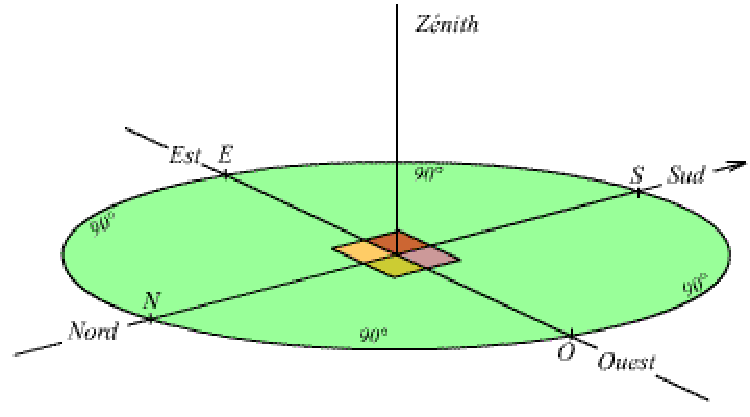
\includegraphics[width=0.4\textwidth]{position}
      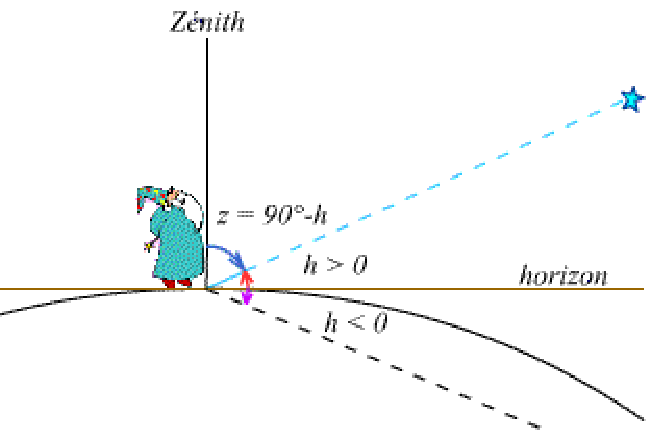
\includegraphics[width=0.4\textwidth]{position2}
    \end{center}
    \label{position}
    \label{position2}
    \caption{G.: Points cardinaux. Dr.: Horizon et distance zénithale.}
  \end{figure}
\end{Answer}

\section{Mouvement diurne}

\begin{Exercise}
  \begin{enumerate}
  \item Dans quelle direction se trouve un astre au moment de sa
    culmination en un lieu de latitude $+50\deg$?
  \item Même question pour un lieu situé à l'équateur.
  \item La hauteur d'un astre varie-t-elle au cours du mouvement
    diurne au pôle Nord?
  \end{enumerate}
\end{Exercise}

\begin{Answer}
  \begin{enumerate}
  \item Lors du mouvement diurne, la culmination d'un astre se produit
    lorsque sa hauteur est maximale.  Suivant sa position de l'objet
    sur la sphère céleste (donc sa déclinaison), l'astre passera entre
    le zénith et le pôle (Nord pour un habitant de l'hémisphère nord
    et Sud pour ...) soit entre le zénith et l'horizon opposé au pôle
    visible. À la latitude de $50\deg$, les étoiles dont la
    déclinaison est plus petite que la latitude, la culmination se
    fera du côté Sud de l'observateur.  Pour les autres étoiles, la
    culmination sera du côté Nord (Fig.~\ref{mouvementdiurne2})

    \begin{figure}[htp]
      \centering
      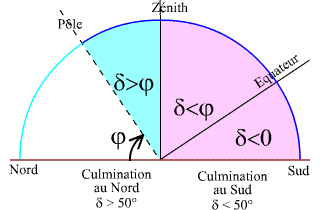
\includegraphics[width=0.3\textwidth]{mouvement_diurne2}
      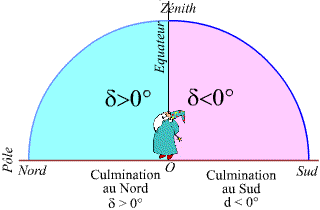
\includegraphics[width=0.3\textwidth]{mouvement_diurne3}
      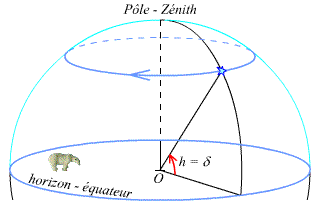
\includegraphics[width=0.3\textwidth]{mouvement_diurne4}
      \label{mouvementdiurne2}
      \label{mouvementdiurne3}
      \label{mouvementdiurne4}
      \caption{Mouvement diurne à une latitude $\phi\sim 50\deg$
        (à g.), à l'équateur ($\phi = 0$, au c.) et au pôle nord
        ($\phi = 90\deg$, à dr.).}
    \end{figure}

  \item L'équateur passant par le zénith, toutes les étoiles de
    déclinaisons positives culminent au Nord et les étoiles de
    déclinaisons négatives au Sud. Les étoiles de déclinaisons nulles
    passent au zénith (Fig.~\ref{mouvementdiurne3}).

  \item La verticale étant confondue avec l'axe du pôle, et l'horizon
    avec l'équateur, la déclinaison est égale à la hauteur de l'astre
    qui reste constante lors de la rotation diurne.  Seuls les objets
    de déclinaisons positives sont visibles. C'est pourquoi le Soleil
    dans son mouvement apparent durant l'année donne 6 mois
    consécutifs de jour et 6 mois consécutifs de nuit
    (Fig.~\ref{mouvementdiurne4}).
  \end{enumerate}
\end{Answer}

\begin{Exercise}[Mouvement diurne des étoiles]
  \begin{enumerate}
  \item Comment varie l'azimut d'un astre au cours du mouvement
    diurne, en un lieu de latitude $50\deg$ ? Et aussi $-50\deg$ de
    latitude. Sur la Fig.~\ref{mouvementdiurne}, on a représenté la
    situation en un lieu de l'hémisphère Sud (latitude = $-50\deg$) ;
    $P$ est alors en-dessous de l'horizon et $P'$ est au-dessus.

    \begin{figure}[htp]
      \centering
      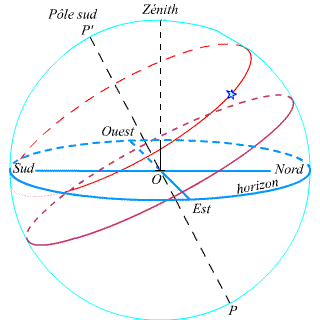
\includegraphics[width=0.5\textwidth]{mouvement_diurne}
      \label{mouvementdiurne}
      \caption{Rotation d'une étoile vue de l'hémisphère sud (latitude =
        $-50\deg$).}
    \end{figure}

  \item Les astres se lèvent-ils du côté de l'Est et se couchent-ils
    du côté de l'Ouest aussi bien dans l'hémisphère Nord que dans
    l'hémisphère Sud?
  \item Dans quelle direction géographique un astre culmine-t-il en un
    lieu de latitude $-50\deg$ ?
  \item Le mouvement diurne est-il observé dans le même sens pour un
    observateur de l'hémisphère Nord ou un observateur de l'hémisphère
    Sud?
  \end{enumerate}
\end{Exercise}

\begin{Answer}
  \begin{enumerate}
  \item
    \begin{description}
    \item[Observateur de l'hémisphère Nord (latitude $+50\deg$)] On
      n'envisagera que le cas des étoiles visibles par l'observateur,
      c'est-à-dire celles dont $\delta > -(\pi/2 - \phi)$. Deux
      critères sont a envisager :
      \begin{itemize}
      \item l'étoile a une déclinaison plus grande que la latitude
        $\delta>\phi$ ou $\delta<\phi$
      \item l'étoile est circumpolaire $\delta > \pi/2 - \phi$
      \end{itemize}
      Par la première condition, si $\delta<\phi$, l'azimut de
      l'étoile varie de 0 à $360\deg$, sinon, son azimut oscille
      entre une valeur comprise $\alpha$ entre 90 et $180\deg$
      suivant sa position au passage au méridien et
      $360\deg-\alpha$. L'étoile oscille donc entre $\alpha$,
      $180\deg$ et $360\deg-\alpha$.

      Le deuxième critère (circumpolarité) indique si l'étoile a un
      lever ou un coucher, son azimut varie alors entre les positions
      des levers et couchers et celles définies par le premier
      critère.

      L'observateur orienté vers le Nord voit tourner les étoiles dans
      le sens direct autour du pôle Nord.

    \item[Observateur de l'hémisphère Sud (latitude $-50\deg$)] Les
      mêmes critères s'appliquent pour les limitations des azimuts et
      des levers et couchers, à la différence que l'azimut va osciller
      autour de la valeur $0\deg$ et que regardant le pôle Sud, il
      verra tourner les étoiles dans le sens rétrograde
      (Fig.\ref{mouvementdiurne}).
    \end{description}
  \item Oui. Que l'on soit dans l'hémisphère Nord ou Sud, le sens de
    rotation de la Terre est le même. Les objets apparaissent à l'Est
    et se couchent à l'Ouest.

  \item Au Nord si sa déclinaison est plus grande que la latitude,
    autrement au Sud (Voir exercice 1 du même chapitre).

  \item Non (Voir exercice 4 du chapitre II).
  \end{enumerate}
\end{Answer}

\begin{Exercise}[Coordonnées horaires d'un astre]
  \begin{enumerate}
  \item Quelle est la relation entre la déclinaison et la distance
    polaire?
  \item Quelles sont les coordonnées horaires des quatre points
    cardinaux en un lieu de latitude $\phi$?
  \item Que vaut la déclinaison du zénith en fonction de la latitude
    du lieu?
  \end{enumerate}
\end{Exercise}

\begin{Answer}
  \begin{enumerate}
  \item Comme son nom l'indique, la distance polaire est l'angle entre
    la direction du pôle nord et la direction de l'objet, donc
    $p=90\deg-\delta$

  \item Table~\ref{tbl:coordonnees_horaire} et
    Fig.~\ref{coordonneeshoraire}

    \begin{center}
      \begin{tabular}{|c|c|c|}
        \hline
        Points cardinaux & Angle horaire & Déclinaison \\ \hline
        Sud   & 0h  & -(90 - $\phi$) \\ \hline
        Ouest & 6h  & 0 degré \\ \hline
        Nord  & 12h & 90 - $\phi$ \\ \hline
        Est   & 18h & 0 degré \\ \hline
      \end{tabular}
      \label{tbl:coordonnees_horaire}
    \end{center}

    \begin{figure}[htp]
      \centering
      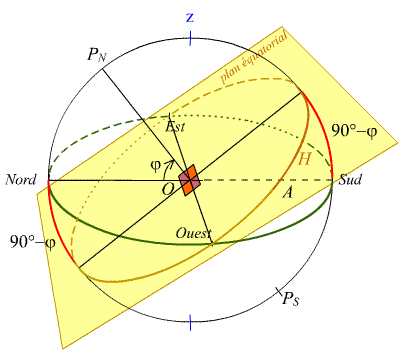
\includegraphics[width=0.45\textwidth]{coordonnees_horaire}
      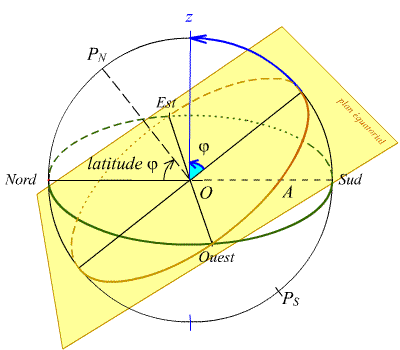
\includegraphics[width=0.45\textwidth]{coordonnees_horaire2}
      \label{coordonneeshoraire}
      \label{coordonneeshoraire2}
      \caption{Coordonnées horaires des points cardinaux (à g.) et du
        zénith (à dr.).}
    \end{figure}

  \item La déclinaison du zénith vaut la latitude (positive pour
    l'hémisphère Nord et négative pour l'hémisphère Sud), cf. Fig.
    \ref{coordonneeshoraire2}.
  \end{enumerate}
\end{Answer}

\begin{Exercise}[Coordonnées équatoriales]
  \begin{enumerate}
  \item Une étoile traverse le méridien sud à une hauteur de
    $85\deg$, et le méridien nord à $45\deg$. Trouver la
    déclinaison de l'étoile et la latitude de l'observateur.
  \item Où ces affirmations sont-elles vraies?
    \begin{enumerate}
    \item Castor ($\alpha$-Gem, déclinaison $+31\deg54'$) est
      circumpolaire.
    \item Bételgeuse ($\alpha$-Ori, $7\deg24'$) culmine au
      zénith.
    \item $\alpha$-Cen ($-60\deg46'$) s'élève à une hauteur de
      $20\deg$ au méridien.
    \end{enumerate}
  \end{enumerate}
\end{Exercise}

\begin{Answer}
  \begin{enumerate}
  \item L'étoile tournant autour de la direction du pôle, les deux
    directions $OA$ et $OB$ des passages supérieur et inférieur, sont
    symétriques par rapport à l'axe $OP$. L'angle $\alpha$ égale
    l'angle $\beta$ et
    $$
    \alpha + \beta+180\deg - 45\deg -85\deg = 50\deg
    \quad\to\quad
    \alpha=\beta=25\deg
    $$
    $\alpha$ et $\beta$ sont tous deux les compléments de la
    déclinaison de l'étoile:
    $$
    \beta+\delta = 90\deg
    \quad\to\quad
    \delta=65\deg
    $$
    On calcule la latitude qui vaut la hauteur du pôle au dessus de
    l'horizon: $\phi=\alpha+45\deg=70\deg$.

    \begin{figure}[htp]
      \centering
      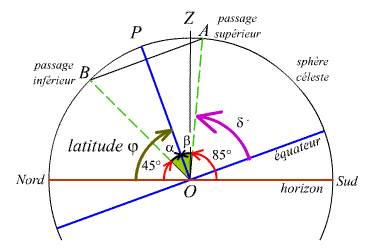
\includegraphics[width=0.5\textwidth]{coordonnees_horaire3}
      \label{coordonneeshoraire3}
      \caption{Coordonnées horaires.}
    \end{figure}

  \item
    \begin{description}
    \item[Castor (Gem, $\delta = +31\deg56'$) circumpolaire]
      L'étoile sera juste circumpolaire, c'est-à-dire passera tangent
      à l'horizon Nord, si sa déclinaison est le complément de la
      latitude.  Pour toute latitude plus grande, l'étoile sera plus
      élevée sur l'horizon et ne disparaîtra pas derrière celui-ci
      (Fig \ref{castor}): $\phi>=90\deg-\delta$
      \begin{figure}[htp]
        \centering
        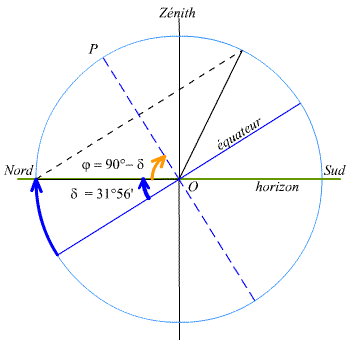
\includegraphics[width=0.3\textwidth]{castor}
        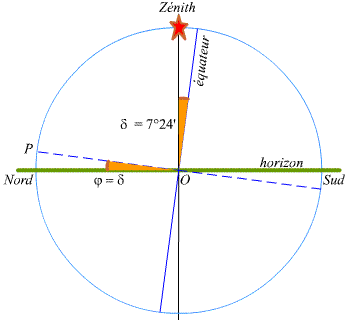
\includegraphics[width=0.3\textwidth]{betelgeuse}
        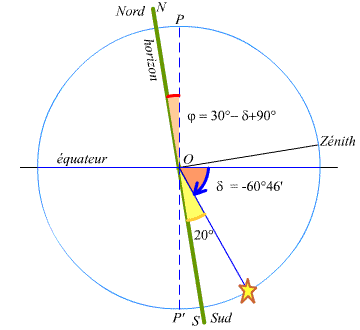
\includegraphics[width=0.3\textwidth]{cen}
        \label{castor}
        \label{betelgeuse}
        \label{cen}
        \caption{Castor (à g.), Bételgeuse (au c.), et
          $\alpha$-Cen. (à dr.).}
      \end{figure}

    \item[Bételgeuse (Ori, $\delta = +7\deg24'$) culmine au zénith]
      Si l'étoile est au moment de sa culmination au zénith
      (nécessairement), sa déclinaison est égale à la latitude
      (Fig.~\ref{betelgeuse}): $\phi=7\deg24'$

    \item[$\alpha$-Cen ($\delta = - 60\deg46'$) s'élève à une
      hauteur de $+20\deg$] À son passage supérieur, l'étoile se
      trouve dans la configuration Fig.~\ref{cen}.  La latitude est
      l'angle $PON$ qui est égal à $P'OS$. En appliquant la relation
      de Chasles entre $P'OS$ la hauteur de l'astre $20\deg$ et la
      déclinaison, on obtient: $P'OS=90\deg+\delta-20\deg$ d'où
      $\phi = 9\deg14'$
    \end{description}
  \end{enumerate}
\end{Answer}

\section{Mouvement du Soleil}

\subsection{Année sidérale, année tropique }

\begin{Exercise}[Mouvement du Soleil, jour solaire]
  \begin{enumerate}
  \item Que valent la hauteur maximale et la hauteur minimale du
    Soleil en chacun des lieux considérés : $50\deg$, $75\deg$,
    $10\deg$, $20\deg$?

  \item À quelle condition doit satisfaire la latitude d'un lieu pour
    que le Soleil n'ait ni lever ni coucher?

  \item Comment comprendre l'expression « soleil de minuit » ?

  \item À quelle condition doit satisfaire la latitude d'un lieu pour
    que le Soleil puisse passer à son zénith?

  \item Comment comprendre l'expression « tropique du Cancer » et «
    tropique du Capricorne » ? on pourra discuter cette question, en
    particulier, en consultant une carte céleste.
  \end{enumerate}
\end{Exercise}

\begin{Answer}
  \begin{enumerate}
  \item Inclinaison de l'écliptique sur l'équateur:
    $\epsilon=23\deg27'$. On détermine les relations qui relient la
    latitude $\phi$, les hauteurs minimum et maximum avec les deux
    positions du Soleil en déclinaison $\pm \epsilon$.
    \begin{itemize}
    \item Position solstice hiver: $SOm = SOE - \epsilon =
      (90\deg-\phi) -\epsilon$
    \item Position solstice été: $SOm = SOE + \epsilon =
      (90\deg-\phi) +\epsilon$
    \end{itemize}
    ou le supplément si le Soleil sous les tropiques est passé de
    l'autre côté.
    \begin{center}
      \begin{tabular}{|c|c|c|c|c|}
        \hline
        Latitude $\epsilon$ & $50\deg$ & $75\deg$ & $10\deg$ &
        $-20\deg$ \\
        \hline
        Hauteur max. & $67\deg27'$ & $38\deg27'$ & $90\deg$ &
        $90\deg$ \\
        \hline
        Hauteur min. & $16\deg33'$ & $-08\deg27'$ & $56\deg33'$
        & $46\deg33'$ \\
        \hline
      \end{tabular}
    \end{center}
    Attention aux positions entre les tropiques, le Soleil au solstice
    d'été pour les latitudes nord (solstice d'hiver pour les latitudes
    sud) est passé au Sud (au Nord) et de ce fait est plus bas que le
    jour où il passe au zénith au méridien (Fig.~\ref{mvtsolaire}).

    \begin{figure}[htp]
      \centering
      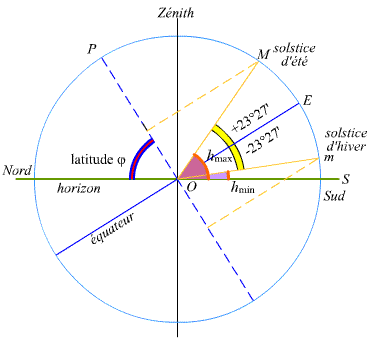
\includegraphics[width=0.5\textwidth]{mvt_soleil}
      \label{mvtsolaire}
      \caption{}
    \end{figure}

  \item Ceci se produit dans l'hémisphère nord en été quand le Soleil
    a une déclinaison suffisamment positive. On appelle ce phénomène
    le « soleil de minuit ». Sur la figure ci-contre (cas de
    l'hémisphère Nord), lorsque au passage inférieur, l'angle $NOD$
    est positif, le Soleil ne se couche pas, son mouvement est
    circumpolaire.
    \begin{eqnarray*}
      NOD = NOE' + E'OD > 0 \\
      90\deg - \phi < \delta_{soleil} \\
      \phi > 90\deg - \delta_{soleil}
    \end{eqnarray*}
    Au jour des solstices ($\delta_{soleil} = \pm 23\deg27'$) il
    suffit d'être à une latitude $\phi > 66\deg33'$ (en été pour
    l'hémisphère Nord) ou $\phi < - 66\deg33'$ (en hiver pour
    l'hémisphère Sud) ; les lieux de latitude $\phi$ égale à $\pm
    66\deg33'$ définissent sur le globe terrestre les parallèles
    appelés « cercles polaires » (respectivement boréal et austral)
    (Fig.~\ref{mvtsolaire2}).

    \begin{figure}[htp]
      \centering
      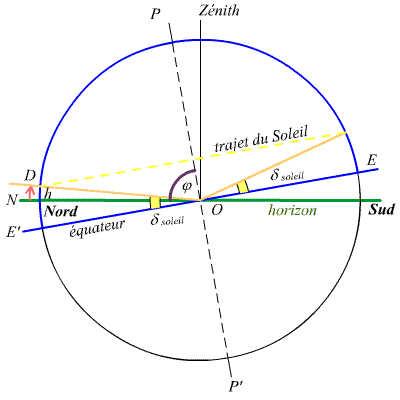
\includegraphics[width=0.5\textwidth]{mvt_soleil2}
      \label{mvtsolaire2}
      \caption{}
    \end{figure}

  \item Vers les pôles, lors de son passage inférieur dans le plan
    méridien, le Soleil est au-dessus de l'horizon et son angle
    horaire ayant augmenté de $180\deg$ depuis sa culmination (par
    définition, il s'agit alors de « midi », 0h temps solaire) vaut
    12h, cela correspond bien à « minuit ». À noter que le Soleil de
    minuit s'observe au Nord dans l'hémisphère boréal et au Sud dans
    l'hémisphère Sud.

  \item Pour que le Soleil passe au zénith, il faut que la déclinaison
    du zénith (qui est aussi la latitude du lieu) soit égale à celle
    du Soleil; comme cette dernière ne peut varier qu'entre
    $+23\deg27'$ et $-23\deg27'$, les lieux en question sont ceux
    de latitude comprise entre $-23\deg27'$ et $+23\deg27'$. Le
    Soleil passe au zénith de ces lieux deux fois dans le cours d'une
    année, au printemps et en été dans l'hémisphère Nord et en automne
    et en hiver dans l'hémisphère Sud. Les zones de la Terre qui
    correspondent à cette propriétés sont appelées les zones
    tropicales car situées entre le tropique nord du Cancer et le
    tropique sud du Capricorne.

  \item Pour les lieux de latitude égale à $+23\deg27'$ et
    $-23\deg27'$, le Soleil passe au zénith au moment des
    solstices. Ces lieux définissent sur le globe terrestre les
    parallèles appelés « tropiques » (du Cancer pour l'hémisphère Nord
    et du Capricorne pour l'hémisphère Sud). Si l'on se reporte à une
    carte du ciel, on voit qu'au moment des solstices le Soleil se
    trouve dans la direction de la constellation des Gémeaux (été) ou
    du Sagittaire (hiver). Il faudrait donc désigner les lieux en
    question par les noms : « tropique des Gémeaux » au lieu de
    tropique du Cancer et de même « tropique du Sagittaire » au lieu
    de tropique du Capricorne. L'appellation en usage a été définie il
    y a environ 3000 ans à une époque où le point gamma était dans la
    direction de la constellation du Bélier ; au solstice d'été le
    Soleil était bien dans la direction du Cancer et au solstice
    d'hiver dans la direction du Capricorne. Ce glissement est produit
    par la précession des équinoxes au rythme de $360\deg$ pour 26
    000 ans, ce qui donne un effet de $42\deg$, (soit environ un
    angle de 3h) sur 3 000 ans, comme on peut le lire sur la carte.
\end{enumerate}
\end{Answer}

\end{document}

%%% Local Variables:
%%% mode: latex
%%% TeX-PDF-mode : 0
%%% ispell-local-dictionary: "francais"
%%% End:
"' pour une version sans
% les solutions.

\documentclass[a4paper,10pt]{report}

% PREAMBULE ==============================

\usepackage[T1]{fontenc}
\usepackage[utf8]{inputenc}
\usepackage[ec]{aeguill}
\usepackage{ae}
\usepackage[cm]{fullpage}
\usepackage[francais]{babel}
\usepackage{amsmath}
\usepackage{multirow}

\usepackage[pdftex]{graphicx}
\graphicspath{{./Figures/}}

%\usepackage[backref,colorlinks=true,breaklinks=true,
%a4paper,bookmarks=false,linktocpage=true]{hyperref}
\usepackage[colorlinks=true]{hyperref}
\hypersetup{
  pdftitle   = Fascicule de TD,
  pdfauthor  = Astro L2,
  pdfsubject = Astrophysique,
}

% Définition de l'environnement 'Exercise'
\newcounter{noexo}
\setcounter{noexo}{0}
\newenvironment{Exercise}[1][]{%
  \stepcounter{noexo}
  \medskip\noindent\textbf{Exercice~\thenoexo~:~#1}
  \medskip\par
  \addcontentsline{toc}{subsubsection}{Exercice~\thenoexo~:~#1}
}{}

% Définition de l'environnement 'Answer'
\usepackage[usenames,dvipsnames]{color}
\usepackage{comment}
\specialcomment{Answer}{%
  \begingroup
  \sffamily\color{CadetBlue}
  \medskip\noindent\textbf{Corrigé :~}
  }{%
  \endgroup}

% Inclusion ou non des corrigés
\ifdefined\sanscorrige
  \message{Fascicule sans solutions}%
  \excludecomment{Answer} % Remove answers
\else
  \message{Fascicule *AVEC* solutions}%
\fi

% Définitions locales
\renewcommand{\d}{\ensuremath{\mathrm{d}}}
\newcommand{\UA}{\ensuremath{\textrm{UA}}}
\renewcommand{\deg}{\ensuremath{^{\circ}}}
\renewcommand{\vec}[1]{\ensuremath{\boldsymbol{#1}}}
\renewcommand{\u}[1]{\ensuremath{\mathrm{#1}}} % Unités

% PAGE DE TITRE ET PREAMBULE ==============================

\makeatletter
\def\thickhrulefill{\leavevmode \leaders \hrule height 1pt\hfill \kern \z@}
\renewcommand{\maketitle}{\begin{titlepage}%
    \let\footnotesize\small
    \let\footnoterule\relax
    \parindent \z@
    \reset@font
    \null
    \begin{center}
      \huge \bfseries \@title
      \ifdefined\sanscorrige
      \else
      \\\textcolor{red}{avec solutions}
      \fi
    \end{center}
    \hrule height 1pt
    \begin{flushright}
      Université Claude Bernard Lyon1 \\
    \end{flushright}
    \vfil
    \vfil
    \begin{figure}[htp]
      \centering
      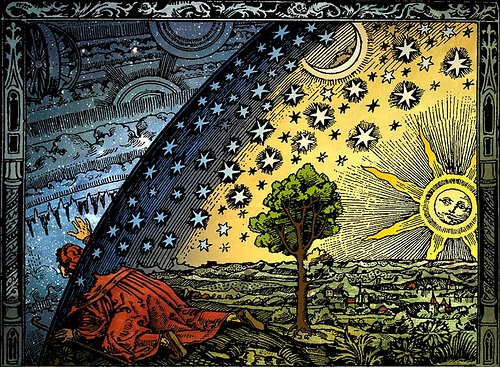
\includegraphics[width=0.8\textwidth]{flammarion}
      \caption{La gravure sur bois dite « de Flammarion »}
    \end{figure}
    \begin{center}
    \vfil
      {\Large \@author} \\[1em]
      {\large \@date}
    \end{center}
  \end{titlepage}%
  \setcounter{footnote}{0}%
}
\makeatother

\title{Fascicule de TD}
\date{Université Lyon 1}
\author{Astrophysique pour la licence}

\begin{document}

\maketitle

% 2: Down to subsection (no exercices)
% 3: Down to subsubsection (exercices)
\setcounter{tocdepth}{2}
\tableofcontents

\newpage

% EXERCICES ET SOLUTIONS ==============================

\chapter{Vie des étoiles}

\section{La lumière des étoiles}

\subsection{Notion de photométrie}

\begin{Exercise}[Dilution du flux avec la distance]
  Réécrire la relation entre la luminosité d'une étoile et le flux
  observé (équation 2.4) dans le cas où la luminosité $L(t)$ dépend du
  temps (par exemple parce que l'étoile est variable) et donc le flux
  observé $F(D,t)$ dépend du temps et de la distance.
\end{Exercise}

\begin{Answer}
  Lorsque la luminosité $L(t)$ de l'étoile dépend du temps, les
  variations de luminosité mettent un temps $D/c$ pour parvenir à un
  observateur situé à une distance $D$ ($c$ étant la vitesse de la
  lumière). Dans ce cas la relation (2.4) devient: $L(t) = 4 \pi D^2
  F(D,t-D/c) $.
\end{Answer}

\subsection{Photosphère et température effective}

\begin{Exercise}[Température effective d'une étoile]
  Calculer la température effective du Soleil à partir de sa
  luminosité $L_{\odot}\approx 3.83\times 10^{26}$~W et de son rayon
  $R_{\odot}\approx 6.96 \times 10 ^{8}$~m.
\end{Exercise}

\begin{Answer}
  En appliquant l'équation :
  $$
  T_e = \left( \frac{L}{4 \pi \sigma R^2_p} \right)^{1/4}
  $$
  avec la constante de Stefan $\sigma = 5.67 \times
  10^{-8}$~\u{Wm^{-2}K^{-4}}, on trouve la température effective du
  Soleil $T_\odot \approx 5770$~K.
\end{Answer}

\subsection{Système de magnitudes}

\begin{Exercise}[Indices de couleur]
  Les deux composantes de l'étoile $\alpha$ du Centaure située à
  1,32~pc de distance ont des magnitudes visuelles (magnitude
  apparente dans la bande $V$) de 0,30 et 1,70. On demande :
  \begin{enumerate}
  \item Le rapport des flux des deux étoiles dans la bande $V$.
  \item La magnitude visuelle globale du système.
  \item La correction qu'il faut apporter aux magnitudes apparentes de
    ce système pour obtenir les magnitudes absolues.
  \end{enumerate}
\end{Exercise}

\begin{Answer}
  On rappelle que la magnitude apparente $m$ est liée au flux $F$ par
  $m = -2,5 \log_{10}(F / F_{0})$.
  \begin{enumerate}
  \item Le rapport des flux des deux composantes de $\alpha$ du
    Centaure dépend de la différence de magnitudes et vaut :
    $$
    F_2 / F_1 = 10^{(m_{1} - m_{2})/2,5} = 0,28
    $$
  \item Pour obtenir la magnitude visuelle globale du système $m_{tot}$,
    il faut calculer le flux total (les puissances émises par les deux
    composantes s'ajoutent) :
    $$
    m_{tot} = -2,5 \log(F_{1} / F_{0} + F_{2} / F_{0})
    $$
    donc
    $$
    m_{tot}= -2,5 \log(10^{-m_{1}/2,5} + 10^{-m_{2}/2,5}) = 0.04
    $$
  \item La correction qu'il faut apporter aux magnitudes apparentes
    $m$ de ce système pour obtenir les magnitudes absolues $M$ vaut:
    $$
    m - M = 5 \log(D/10 \u{pc}) = -4,4
    $$
  \end{enumerate}
\end{Answer}

\section{Évolution stellaire}

\subsection{Formation des étoiles}

\begin{Exercise}
  Quelle est la source de l'énergie rayonnée par:
  \begin{enumerate}
  \item une proto-étoile?
  \item une étoile?
  \item une naine brune?
  \end{enumerate}
\end{Exercise}

\begin{Answer}
  L'énergie rayonnée provient de:
  \begin{enumerate}
  \item l'énergie gravitationnelle pour une proto-étoile ;
  \item l'énergie produite par les réactions nucléaires pour une
    étoile (fusion de H sur la séquence principale, fusion de He ou de
    C et O ensuite, selon la masse de l'étoile) ;
  \item l'énergie gravitationnelle pour une naine brune, qui continue
    à se contracter, ne passant jamais de la proto-étoile à l'étoile.
  \end{enumerate}
\end{Answer}

\subsection{Séquence principale}

\begin{Exercise}
  Quel est le phénomène marquant:
  \begin{enumerate}
  \item le début de la séquence principale?
  \item sa fin?
  \end{enumerate}
\end{Exercise}

\begin{Answer}
  La séquence principale débute quand les réactions de fusion de
  l'hydrogène s'allument dans le coeur de la proto-étoile, et se
  termine lorsque la fusion de l'hydrogène cesse au centre (elle peut
  continuer dans une couche autour d'un noyau d'hélium ou cesser dans
  toute l'étoile selon sa masse).
\end{Answer}

\subsection{Évolution post-SP}

\begin{Exercise}[Étoile de $M > 5 M_{\odot}$]
  Que se passe-t-il si un combustible s'épuise au centre d'une étoile?
\end{Exercise}

\begin{Answer}
  Quand un combustible s'épuise au centre d'une étoile, les réactions
  de fusion de cet élément cessent dans le coeur, mais peuvent
  continuer autour, dans une couche où le combustible est toujours
  présent. Au centre, il n'y a plus de production d'énergie pour
  soutenir le coeur, la gravité l'emporte et le coeur se
  contracte. Cette contraction provoque une augmentation de
  température qui, si elle est suffisante (cela dépend de la masse de
  l'étoile), permet d'allumer de nouvelles réactions nucléaires ayant
  pour combustible le produit des réactions précédentes.
\end{Answer}

\section{Classification spectrale}

\subsection{Mesures des distances}

\subsubsection{Parallaxe trigonométrique}

\begin{Exercise}
  Relier l'incertitude sur la distance $\Delta d$ à celle sur la
  parallaxe $\Delta p$.
\end{Exercise}

\begin{Answer}
  Il existe deux méthodes pour trouver le résultat demandé:
  \begin{itemize}
  \item En différenciant l'équation $d = a/p$, on obtient $\d d =
    -(a/p^2)\d p$, d'où l'incertitude en prenant la valeur absolue:
    $$
    \Delta d = \frac{a}{p^2}\Delta p = \frac{d}{p}\Delta p
    $$
    On a finalement
    $$
    \frac{\Delta d}{d} = \frac{\Delta p}{p}
    $$

  \item On peut également prendre le logarithme de l'équation $d =
    a/p$, ce qui donne $\ln~d = \ln~a - \ln~p$, puis on différencie:
    $\d\ln~d = -\d\ln~p$, soit $\d d/d = -\d p/p$. En prenant la
    valeur absolue, on retrouve le résultat sur l'incertitude:
    $$
    \frac{\Delta d}{d} = \frac{\Delta p}{p}
    $$
  \end{itemize}
\end{Answer}

\begin{Exercise}
  Imaginons deux missions spatiales: FAME et GAIA. Quelles seraient
  les précisions obtenues à une distance de 100~pc? de 1000~pc?  À
  quelle distance aura-t-on une erreur de 100\%?

  On donne les incertitudes absolues sur les parallaxes pour chaque
  satellite:
  \begin{itemize}
  \item $\Delta p=50~\mu as$ pour FAME et
  \item $\Delta p=4~\mu as$ pour GAIA.
  \end{itemize}
\end{Exercise}

\begin{Answer}
  Les étoiles situées à $d=100$~pc ont une parallaxe
  $p=1/100=0,01''=10$~mas. La précision obtenue avec FAME sera de
  $$
  \frac{\Delta d}{d} = \frac{\Delta p}{p} = \frac{50 \times
    10^{-6}}{10^{-2}} = 5 \times 10^{-3} = 0.5 \%
  $$
  et de
  $$
  \frac{\Delta d}{d} = \frac{\Delta p}{p} = \frac{4 \times
    10^{-6}}{10^{-2}} = 4 \times 10^{-4} = 0.04 \%
  $$
  avec GAIA.

  Pour des étoiles à $d=1000$~pc, $p=1$~mas, et les précisions
  deviennent 10 fois moins bonnes: 5\% avec FAME et 0,4\% avec GAIA.

  On aura une erreur de 100\% quand $\Delta d =d$, soit $\delta p =
  p$. La distance correspondante s'obtient donc par
  $$
  d = \frac{1}{p} = \frac{1}{50 \times 10^{-6}} = 20~\u{kpc}
  \quad\text{avec FAME}
  $$
  et
  $$
  d = \frac{1}{p} = \frac{1}{4 \times 10^{-6}} = 250~\u{kpc}
  \quad\text{avec GAIA}
  $$
\end{Answer}


\begin{Exercise}
  Le tableau suivant donne la magnitude apparente $m_V$ et la
  parallaxe $p$ de trois étoiles. Calculer leur distance $d$ avec son
  incertitude, l'erreur relative sur la distance $\Delta d / d$ et
  leur magnitude absolue $M_V$.
  \begin{center}
    \begin{tabular}{|c|c|c|c|}
      \hline
      & $\alpha$ CMa Sirius & $\alpha$ Tau Aldebaran & $\alpha$ Ori
      Bételgeuse \\
      \hline
      $m_V$ & -1.47 & 0.85 & 0.58 \\
      \hline
      $p$ (mas) & 379.2 $\pm$ 1.6 & 50.1 $\pm$ 1.0 & 7.6 $\pm$ 1.6 \\
      \hline
      $d$ (pc) &   &   &  \\
      \hline
      $\Delta d / d$ &   &   &  \\
      \hline
      $M_V$ &   &   &  \\
      \hline
    \end{tabular}
  \end{center}
\end{Exercise}

\begin{Answer}
  \begin{center}
    \begin{tabular}{|c|c|c|c|}
      \hline
      & $\alpha$ CMa Sirius & $\alpha$ Tau Aldebaran & $\alpha$ Ori
      Bételgeuse \\
      \hline
      $m_V$ & -1.47 & 0.85 & 0.58 \\
      \hline
      $p$ (mas) & 379.2 $\pm$ 1.6 & 50.1 $\pm$ 1.0 & 7.6 $\pm$ 1.6 \\
      \hline
      $d$ (pc) &  \color{red}{2.64 $\pm$ 0.01} &  \color{red}{20.0
        $\pm$ 0.4}  & \color{red}{130 $\pm$ 30} \\
      \hline
      $\Delta d / d$ & \color{red}{0.4\%}  & \color{red}{2\%}  &
      \color{red}{23\%} \\
      \hline
      $M_V$ & \color{red}{1.42}  & \color{red}{-0.65}  &
      \color{red}{-4.99} \\
      \hline
    \end{tabular}
  \end{center}

  Étant donné la forme de la relation donnant la distance $d$ à partir
  de la parallaxe $p$, leurs incertitudes relatives sont égales, ce
  qui permet d'avoir immédiatement $\Delta d / d$. Ces résultats
  illustrent bien la diminution de la précision lorsque la distance
  augmente.

  La magnitude absolue s'obtient par la relation $M_V = m_V - 5~\log~d
  + 5$.
\end{Answer}


\begin{Exercise}[Méthode du point convergent]
  On veut déterminer la distance de l'amas des Pléiades par la méthode
  du point convergent.
  \begin{itemize}
  \item L'étude des trajectoires des étoiles de l'amas sur plusieurs
    années a permis de situer le point convergent à $\theta = 67,9 \pm
    0,6\deg$ de la direction de l'amas.
  \item L'observation du spectre de l'étoile Alcyone, faisant partie
    de cet amas, a permis de mesurer sa vitesse radiale $v_r = 10,1
    \pm 0,3$~\u{km.s^{-1}}.
  \item Le mouvement propre apparent de cette même étoile vaut $\mu =
    47,3 \pm 0,8$~\u{mas.an^{-1}}.
  \end{itemize}
  Déterminer la distance de l'amas. Attention aux unités !
\end{Exercise}

\begin{Answer}
  Dans la formule donnant la distance de l'amas, il faut bien faire
  attention à exprimer l'angle $\mu$ en radians et à utiliser les
  mêmes unités de distance et de temps pour les autres grandeurs.
  \begin{itemize}
  \item $\mu = 47,3 \pm 0,8~\u{mas.an^{-1}} = (2,29 \pm 0,04) \times
    10^{-7}~\u{rad.an^{-1}}$
  \item $v_r = 10,1 \pm 0,3~\u{km.s^{-1}} = (1,02 \pm 0,03) \times
    10^{-5}~\u{pc.an^{-1}}$
  \item $\theta = 67,9 \pm 0,6\deg = 1,19 \pm 0,01$~rad
  \item On a donc $tan \theta= 2,50 \pm 0,07$.
  \item Finalement: $d = 111 \pm 8$~pc
  \end{itemize}
\end{Answer}

\subsection{Classification stellaire}

\begin{Exercise}[Types spectraux]
  Donner approximativement le type spectral des étoiles dont le flux
  est maximal aux longueurs d'onde suivantes: 300~nm, 500~nm, et
  1,2~$\mu$m.  Peut-on déterminer la classe de luminosité?

  Rappel de la loi de Wien: $\lambda_{\max} T = 2898$~\u{\mu m.K}.
\end{Exercise}

\begin{Answer}
  La loi de Wien permet de déterminer la température effective de
  chaque étoile, et ainsi d'en déduire une valeur approximative du
  type spectral. Ici seulement la première lettre est accessible, la
  détermination du chiffre suivant nécessiterait un tableau plus
  précis donnant les correspondances entre les sous-types et la
  température effective.
  \begin{center}
    \begin{tabular}{|c|c|c|}
      \hline
      $\lambda_m$ & $T_{eff}(K)$ & Type spectral \\
      \hline
      300 nm & \color{red}{9660} & \color{red}{A}  \\
      \hline
      500 nm & \color{red}{5796} & \color{red}{G} \\
      \hline
      1.2 $\mu m$ &  \color{red}{2415} &  \color{red}{M} \\
      \hline
    \end{tabular}
  \end{center}
  On ne peut pas déterminer la classe de luminosité grâce à la
  longueur d'onde du maximum du flux. Pour ceci, il faudrait connaître
  soit la luminosité de l'étoile, soit sa gravité de surface, soit son
  rayon.
\end{Answer}

\begin{Exercise}[Diagramme HR]
  Classer par ordre de température effective croissante, puis de rayon
  croissant, et enfin de luminosité croissante les étoiles de types
  spectraux suivants: M5III, O2V, K7I, A0VII.
\end{Exercise}

\begin{Answer}
  La séquence OBAFGKM décrit les types spectraux dans le sens des
  $T_{eff}$ décroissantes, on aura donc dans le sens des $T_{eff}$
  croissantes: \textcolor{red}{M5III}, \textcolor{red}{K7I},
  \textcolor{red}{A0VII}, et \textcolor{red}{O2V}.

  La classe de luminosité définit des groupes d'étoiles de rayon
  différent, on aura donc dans l'ordre croissant:
  \textcolor{red}{A0VII}, \textcolor{red}{O2V},
  \textcolor{red}{M5III}, et \textcolor{red}{K7I}.

  Enfin, l'examen du diagramme HR montre qu'une étoile chaude de la
  séquence principale peut être plus lumineuse qu'une sous-géante
  froide, et on aura dans le sens des luminosités croissantes:
  \textcolor{red}{A0VII}, \textcolor{red}{M5III},
  \textcolor{red}{O2V}, et \textcolor{red}{K7I}.

  Ceci montre que le terme « classe de luminosité » peut être source
  d'erreur.
\end{Answer}

\subsection{Mesure des rayons}

\begin{Exercise}[Interférométrie]
  Le tableau suivant donne le diamètre apparent $\theta_*$ de quelques
  étoiles, mesuré par interférométrie. Calculer leur rayon $R$ (on
  rappelle les distances déterminées dans un exercice précédent) et, à
  l'aide de ce résultat, attribuer à chaque étoile sa classe de
  luminosité parmi les suivantes: I, III, V.

  \begin{center}
    \begin{tabular}{|c|c|c|c|}
      \hline
      & $\alpha$ CMa Sirius & $\alpha$ Tau Aldebaran & $\alpha$ Ori
      Bételgeuse \\
      \hline
      $\theta_*$ (mas) & 5.89 & 24 & 67 \\
      \hline
      $p$ (mas) & 379.2 $\pm$ 1.6 & 50.1 $\pm$ 1.0 & 7.6 $\pm$ 1.6 \\
      \hline
      $d$ (pc) & 2.64  & 20  & 130 \\
      \hline
      $R (R_{\odot})$ &   &   &  \\
      \hline
      Classe de luminosité &   &   &  \\
      \hline
    \end{tabular}
  \end{center}
\end{Exercise}

\begin{Answer}
  Pour Sirius:
  \begin{itemize}
  \item Son diamètre apparent vaut $\theta_*= 5,89~\u{mas} = 2,86 \times
    10^{-8}$~rad.
  \item Son rayon vaut donc $R = \theta_* d / 2 = 3,8 \times 10^{-8}
    pc = 1,2 \times 10^9 m = 1,7R_{\odot}$.
  \end{itemize}
  Le tableau suivant donne les résultats pour les 3 étoiles:
  \begin{center}
    \begin{tabular}{|c|c|c|c|}
      \hline
      & $\alpha$ CMa Sirius & $\alpha$ Tau Aldebaran & $\alpha$ Ori
      Bételgeuse \\
      \hline
      $\theta_*$ (mas) & 5.89 & 24 & 67 \\
      \hline
      $p$ (mas) & 379.2 $\pm$ 1.6 & 50.1 $\pm$ 1.0 & 7.6 $\pm$ 1.6 \\
      \hline
      $d$ (pc) & 2.64  & 20  & 130 \\
      \hline
      $R (R_{\odot})$ & \color{red}{1.7}  & \color{red}{52}  &
      \color{red}{936} \\
      \hline
      Classe de luminosité & \color{red}{V}  & \color{red}{III}  &
      \color{red}{I} \\
      \hline
      Type spectral & A1V  & K5III  & M2I \\
      \hline
    \end{tabular}
  \end{center}
  Dans cet exemple, il est possible d'attribuer à chaque étoile sa
  classe de luminosité en utilisant le lien qui existe avec le rayon
  stellaire. Le type spectral complet est donné pour information.
\end{Answer}

\subsection{Mesure de masse}

\subsubsection{Étoiles doubles}

\begin{Exercise}
  On observe une étoile double visuelle dont le plan de l'orbite est
  perpendiculaire à la ligne de visée.
  \begin{itemize}
  \item La parallaxe de ce système est de 100~mas.
  \item La plus grande séparation angulaire entre les deux composantes
    est de $5''$, et la plus petite de $1''$.
  \item La période de révolution est de 30~ans.
  \item L'étoile primaire se trouve au foyer de l'orbite observée, car
    il n'y a pas d'effet de projection.
  \item Le compagnon est toujours observé à une distance du centre de
    gravité 5~fois plus grande que celle de l'étoile primaire.
  \end{itemize}

  Déterminer la masse de chaque composante.
\end{Exercise}

\begin{Answer}
  Les paramètres observés permettent de remonter aux données suivantes
  pour le système:
  \begin{itemize}
  \item La distance est $d = 10$~pc.
  \item La dimension angulaire du grand axe de l'orbite relative est
    de $5'' + 1'' = 6''$. Le demi-grand axe apparent est donc $\theta
    = 3''$, soit $\theta = 1,45 \times 10^{-5} rad$.
  \item Le demi-grand axe de l'orbite relative vaut donc $a = \theta d
    = 1,45 \times 10^{-4} pc = 4,49 \times 10^{12} m = 30 \UA$.
  \item La $3^{ème}$ loi de Kepler donne la somme des masses: $M1 + M2
    = 5,97 \times 10^{31} kg = 30 M_{\odot}$ .
  \item Les distances des étoiles $E_1$ et $E_2$ au centre de gravité
    $G$ vérifient $M_1 \times GE_1 = M_2 \times GE_2$. Le rapport des
    masses vaut donc $M_1 / M_2 = GE_2 / GE_1 = 5$.
  \item Finalement: $M_1 = 25M_{\odot}$ et $M_2 = 5M_{\odot}$
  \end{itemize}
\end{Answer}


\begin{Exercise}
  Le tableau suivant rappelle les caractéristiques du système binaire
  à éclipse d'Algol ($\beta$ Per):
  \begin{center}
    \begin{tabular}{|l|c|r|}
      \hline
      $p$ (mas) &  \multicolumn{2}{c|}{35.1 $\pm$ 0.9} \\
      \hline
      $d$ (pc) & \multicolumn{2}{c|}{28.6 $\pm$ 0.7} \\
      \hline
      $T$ (jours) & \multicolumn{2}{c|}{2.8674} \\
      \hline
      & A & B \\
      \cline{1-3}
      Type spectral & B8V & K2IV \\
      \hline
      R ($R_{\odot}$) & 2.74 & 3.60 \\
      \hline
    \end{tabular}
  \end{center}
  On a mesuré de plus les paramètres orbitaux suivants (on supposera
  l'orbite circulaire, ainsi le demi-grand axe de l'ellipse projetée
  est égal au rayon de l'orbite):
  \begin{center}
    \begin{tabular}{|c|c|}
      \hline
      $\theta$ (mas) & 2.283 \\
      \hline
      $\theta_2$ (pc) & 1.872 \\
      \hline
    \end{tabular}
  \end{center}
  Quelle est la séparation des deux étoiles en km? en UA? en
  $R_{\odot}$? Comparez-la à leurs rayons.

  Quelle est la masse de chacune des étoiles?
\end{Exercise}

\begin{Answer}
  \begin{itemize}
  \item Le demi-grand axe apparent de l'orbite relative est $\theta =
    2.283~mas = 1,11 \times 10^{-8}~rad$.
  \item Le demi-grand axe de l'orbite relative vaut donc $a = \theta d
    = 3,17 \times 10^{-7}~pc = 9,77 \times 10^9~m = 0,065~\UA =
    14R_{\odot}$.
  \item La 3ème loi de Kepler donne la somme des masses:
    $M_1+M_2 = 4\pi^2 a^3/GT^2 = 8,98 \times 10^{30}~kg =
    4,52M_{\odot}$.
  \item Le rapport des demi-grands axes apparents de l'orbite relative
    $\theta$ et de l'orbite absolue de l'étoile secondaire $\theta_2$
    donne le rapport des masses: $\theta_2 / \theta = a_2 / a = M_1 /
    (M_1 + M_2) = 0,82$
  \item On obtient donc les masses $M_1 = 3,71$ et $M_2 = 0,81$.
  \end{itemize}

  Le tableau suivant récapitule les données physiques du système:
  \begin{center}
    \begin{tabular}{|l|c|r|}
      \hline
      $d$ (pc) & \multicolumn{2}{c|}{28.6 $\pm$ 0.7} \\
      \hline
      $T$ (jours) & \multicolumn{2}{c|}{2.8674} \\
      \hline
      $a$ ($R_{\odot}$) &  \multicolumn{2}{c|}{\color{red}{14}} \\
      \hline
      & A & B \\
      \cline{1-3}
      Type spectral & B8V & K2IV \\
      \hline
      R ($R_{\odot}$) & 2.74 & 3.60 \\
      \hline
      M ($M_{\odot}$) & \color{red}{3.71} & \color{red}{0.81} \\
      \hline
    \end{tabular}
  \end{center}
  On remarque que l'étoile la plus grosse (B) est la moins massive et
  la moins chaude, on peut en déduire que le minimum principal a lieu
  lorsque cette dernière occulte l'étoile A, plus chaude et plus
  lumineuse.

  On constate également que la séparation des étoiles vaut un peu
  moins de 4 fois le rayon de la plus grosse, il s'agit donc d'une
  binaire serrée.
\end{Answer}

\section{Les systèmes planétaires}

\subsection{Les lois de Kepler}

\begin{Exercise}[Enoncé et rappels sur les ellipses]
  L'orbite de Pluton est très excentrique ($e=0,248$). Son demi grand
  axe vaut 39,43~unités astronomiques (L'unité astronomique est
  définie comme le demi grand axe de l'orbite de la Terre). Montrer
  que Pluton peut être plus proche du Soleil que Neptune dont le demi
  grand axe de l'orbite vaut 30,06~UA et l'excentricité 0,009.
\end{Exercise}

\begin{Answer}
  On calcule simplement les distances planète-Soleil pour les deux
  planètes à leur périhélie et à leur aphélie. Si Neptune est repérée
  par le vecteur $\vec{SN}$ et Pluton par le vecteur $\vec{SP}$, on a:
  \begin{itemize}
  \item Au périhélie:
    $$
    SN = a_n(1-e_n) = 30.06 \times (1-0.009) = 29.79~\UA
    $$
    $$
    SP = a_p(1-e_p) = 39.43 \times (1-0.248) = 29.65~\UA
    $$
  \item À l'aphélie:
    $$
    SN = a_n(1+e_n) = 30.06 \times (1+0.009) = 30.33~\UA
    $$
    $$
    SP = a_p(1+e_p) = 39.43 \times (1+0.248) = 49.21~\UA
    $$
  \end{itemize}
  On voit que, du fait de la très grande excentricité de son orbite,
  Pluton, à son périhélie, est plus proche que Neptune du Soleil.
\end{Answer}

\begin{Exercise}[Dérivation des lois de Kepler]
  Montrer que la vitesse angulaire d'un objet décrivant une orbite
  elliptique autour du Soleil augmente lorsqu'il s'en
  rapproche. Montrer que le rapport des vitesses au périhélie (point
  le plus proche du Soleil) et à l'aphélie (point le plus éloigné du
  Soleil) ne dépend que de l'excentricité de l'orbite.  Calculer ce
  rapport pour la Terre dont l'excentricité de l'orbite vaut 0,0167,
  puis pour la comète de Halley dont l'excentricité de l'orbite vaut
  0,97.
\end{Exercise}

\begin{Answer}
  \begin{enumerate}
  \item On a vu que $r^2\dot{\theta}$ est une constante. On a donc
    $\dot{\theta}=C/r^3$ et la vitesse angulaire augmente lorsque $r$
    diminue.

  \item L'expression de la vitesse est: $\vec{v} = \dot{r}\vec{i} +
    r\dot{\theta}\vec{j}$

    Le périhélie et l'aphélie correspondent à des extremum sur la
    trajectoire, c'est à dire que $\d r/\d\theta =0$ et donc,
    puisque $\dot{r} = \dot{\theta}~\d r/\d\theta$,
    $\dot{r}=0$. La vitesse s'écrit donc bien $v = r\dot{\theta}$

  \item Puisque $r^2\dot{\theta}=C$ et que $v = r\dot{\theta}$, on a
    $v = C/r$. En reprenant les résultats vus précédemment sur les
    ellipses, on trouve $r = a(1-e)$ au périhélie, et $r = a(1+e)$ à
    l'aphélie. Le rapport des vitesse $v_p$ au périhélie et $v_a$ à
    l'aphélie est donc:
    $$
    \frac{v_p}{v_a} = \frac{1+e}{1-e}
    $$
    Soit pour la Terre:
    $$
    \frac{v_p}{v_a} = \frac{1+0.0167}{1-0.0167} = 1.034
    $$
    Et pour la comète de Halley:
    $$
    \frac{v_p}{v_a} = \frac{1+0.97}{1-0.97} = 65.67
    $$
  \end{enumerate}
\end{Answer}

\begin{Exercise}
  En reprenant le raisonnement précédent, trouver l'équation de la
  trajectoire d'une planète autour du Soleil si la force de
  gravitation était en $1/r^3$ au lieu de $1/r^2$. En déduire que dans
  ce cas, vous ne seriez pas en train de vous embêter à faire cet
  exercice.
\end{Exercise}

\begin{Answer}
  On reprend l'expression de l'équation différentielle en remplaçant
  $y^2$ dans le membre de droite par $y^3$. On obtient l'équation
  suivante:
  $$
  -C^2 y^2 \left( y + \frac{d^2y}{d \theta ^2} \right) = -G(M_{\odot}
  + M_p)y^3
  $$
  Qui se simplifie par:
  $$
  -C^2 y - C^2 \frac{d^2y}{d \theta ^2} = G(M_{\odot} + M_p)y
  $$
  Qui devient, en réorganisant les différents termes:
  $$
  \frac{d^2y}{d \theta ^2} + \left[ 1 - \frac{ G(M_{\odot} + M_p)
    }{C^2} \right]y = 0
  $$
  Ou encore, en posant $\alpha = \left[ 1 - \frac{ G(M_{\odot} + M_p)
    }{C^2} \right]$
  $$
  \frac{d^2y}{d \theta ^2} + \alpha y = 0
  $$
  Il faut analyser les trois cas $\alpha < 0$, $\alpha > 0$ et $\alpha
  = 0$.
  \begin{description}
  \item[$\alpha > 0$] On pose $\epsilon = \sqrt{\left | \alpha \right |
    }$ et l'équation différentielle s'écrit alors:
    $$
    \frac{d^2y}{d \theta ^2} + \epsilon^2 y = 0
    $$
    dont la solution s'écrit simplement:
    $$
    y = K\cos(\epsilon \theta + \phi)
    $$
    donc:
    $$
    r = \frac{C}{\cos(\epsilon \theta + \phi)}
    $$
    où $C$, $\phi$ et $\epsilon$ sont des constantes. Cette équation a
    une singularité lorsque $\theta = (\pi/2 - \phi) /
    \epsilon$. Lorsque $\theta$ approchera cette valeur, la planète
    s'échappera puisqu'alors $r \to \infty$. La figure (\emph{pas
      trouvé la figure}) montre la trajectoire correspondante pour les
    valeurs des constantes suivantes: $\epsilon = 0.05$, $\phi=0$ et
    $C=1$. La planète arrive à proximité de l'étoile par une des
    branches infinies, et repart par l'autre après avoir décrit
    quelques révolutions autour de l'étoile.

  \item[$\alpha < 0$] Comme précédemment, on réécrit l'équation
    différentielle:
    $$
    \frac{d^2y}{d \theta ^2} + \epsilon^2 y = 0
    $$
    Dont la solution est:
    $$
    y = A e^{\epsilon \theta} + B e^{- \epsilon \theta}
    $$
    donc:
    $$
    r = \frac{1}{A e^{\epsilon \theta} + B e^{- \epsilon \theta}}
    $$
    On voit cette fois que lorsque $\theta$ augmente $r$ diminue
    exponentiellement. la planète s'effondrera donc sur l'étoile.

  \item[$\alpha = 0$] L'équation différentielle a la forme suivante:
    $$
    \frac{d^2y}{d \theta ^2} = 0
    $$
    Dont la solution est:
    $$
    y = A \theta + B
    $$
    donc:
    $$
    r = \frac{1}{A \theta + B}
    $$
    Ici encore, la planète s'effondrera sur l'étoile. On voit donc que
    si la loi de la gravitation était en $\frac{1}{r^3}$, il
    n'existerait pas de trajectoire fermée dans le problème à deux
    corps, et aucune planète ne pourrait graviter autour des étoiles.
  \end{description}
\end{Answer}


\begin{Exercise}
  Sachant que la Lune décrit son orbite autour de la Terre en 27,32
  jours et que le demi grand-axe de son orbite vaut 384400 km,
  calculer l'altitude d'un satellite géostationaire. On supposera que
  la masse de la Lune est négligeable par rapport à celle de la Terre
  (la Terre est environ 80 fois plus massive que la Lune).
\end{Exercise}

\begin{Answer}
  La troisième loi de Kepler, telle que nous venons de la démontrer
  s'applique bien sûr aussi pour le système Terre-Lune et on a:
  $$
  \frac{a^3_L}{T^2_L} = \frac{G(M_T + M_L)}{4\pi^2}
  $$
  Où $a_L$ est le demi grand axe de l'orbite de la Lune, $T_L$ sa
  période orbitale et $M_L$ sa masse. Puisque la masse de la Lune peut
  être négligée par rapport à celle de la Terre, cette relation s'écrit:
  $$
  \frac{a^3_L}{T^2_L} = \frac{GM_T}{4\pi^2}
  $$
  De même, pour le satellite, l'hypothèse $M_S \ll M_T$ est encore plus
  justifiée, et on a:
  $$
  \frac{a^3_S}{T^2_S} = \frac{GM_T}{4\pi^2}
  $$
  et donc:
  $$
  \frac{a^3_S}{T^2_S} = \frac{a^3_L}{T^2_L}
  $$
  La période d'un satellite géostationnaire est, par définition, de 23h56
  heures (car un satellite géostationnaire reste toujours au dessus du
  même point de la Terre dont la période de rotation est de 23h56
  heures). On a donc
  $$
  T_S = 23 \times 60 + 56 = 1435~min
  $$
  $$
  T_L = 27.3 \times 24 \times 60 = 39312~min
  $$
  et
  $$
  \frac{a^3_S}{1435^2} = \frac{384400^3}{39312^2}
  $$
  d'où l'on tire finalement:
  $$
  a_S = 42300~km
  $$
  Cette valeur correspond à la distance entre le centre de la Terre et
  le satellite. L'altitude du satellite est donc:
  $$
  a_S = 42300 - 6378 = 35922~km
  $$
\end{Answer}

% ===============================================================================
\chapter{Vie des galaxies}


\section{Milieu interstellaire}

\subsection{Mise en évidence expérimentale}

\begin{Exercise}
  Dans une observation de comptage d'étoiles, toutes de même type, on
  constate que:
  \begin{itemize}
  \item pour $m\le7$, $\log{N(m)}=0.6 m + 3$
  \item pour $m\ge9$, $\log{N(m)}=0.6 m + 2.4$
  \end{itemize}

  \begin{enumerate}
  \item Déterminer l'extinction en magnitude A due au nuage traversé
    quand on passe de m=7 à m=9.

  \item On sait que la magnitude absolue des étoiles de ce type est
    M=5.  Déterminer :
    \begin{itemize}
    \item La distance $r_{1}$ du front proche du nuage.
    \item L'épaisseur $r_{2}-r_{1}$ du nuage.
    \end{itemize}
  \end{enumerate}
\end{Exercise}

\begin{Answer}
  \begin{enumerate}
  \item L'extinction est nulle jusqu'à la distance $r_1$ du front du
    nuage, donc, avec l'équation :
    $$
    \log{N(m)} = 0.6(m-A) + Cte
    $$
    pour $m=7$:
    $$
    \log{N(m)} = 0.6 (7-0) + 3 = 7.2
    $$

    À la distance $r_2$ du bord éloigné du nuage, pour laquelle $m =
    9$, et l'extinction vaut $A$:
    $$
    \text{pour} m = 9, \log{N(m)} = 0.6(9-A) + 2.4 = 7.8-0.6A
    $$
    d'où $0.6A = 0.6$ et $A = 1$~mag.

  \item En écrivant l'équation du module de distance avec $M=5$ :
    \begin{itemize}
    \item pour $m = 7 = 5\log{r_1} -5 +M$ d'où $r_1 = 25.1$ pc =
      distance du front proche du nuage
    \item pour $m = 9 = 5\log{r_2} -5 +M +1$ d'où $r2 = 39,8$ pc
    \end{itemize}
    Épaisseur du nuage = $r_2-r_1 = 39.8-25.1 = 14.7$ pc
  \end{enumerate}
\end{Answer}

\subsection{Extinction du MIS}

\begin{Exercise}[Interprétation physique]
  Une étoile est située à 2000 pc de l'observateur sur une ligne de
  visée représentative des conditions moyennes du MIS, pour lesquelles
  l'extinction moyenne est de $A_V = 0.3$~mag/kpc.  En admettant que
  cette extinction n'est due qu'à des grains dont les caractéristiques
  suivent :
  \begin{itemize}
  \item rayon $a = 0.1\mu$
  \item $Q_{ext} = 1$
  \item masse volumique : 1~g/cm$^{3}$
  \item répartition des grains uniforme sur la ligne de visée.
  \end{itemize}
  calculer :
  \begin{enumerate}
  \item La densité de colonne des grains le long de la ligne de visée.
  \item Le nombre de grain par unité de volume sur cette ligne de
    visée.
  \item La masse volumique des grains dans le MIS.
  \end{enumerate}

  En admettant que la densité moyenne d'atomes d'Hydrogène est de l'ordre de 8
  atomes par $cm^3$, et en négligeant la présence des atomes d'autres
  éléments, calculer :
  \begin{enumerate}
  \item la masse volumique du gaz dans le MIS.
  \item le rapport (masse volumique des grains)/(masse volumique du
    gaz)
  \item Qu'en concluez vous sur le rôle des grains dans la matière du
    MIS?
  \end{enumerate}
\end{Exercise}

\begin{Answer}
  Distance de l'étoile :
  $$
  L = 2000[\u{pc}] .(3 10^{18} [\u{cm/pc}]) = 6 10^{21} [\u{cm}]
  $$
  Section d'un grain :
  $$
  s_g = \pi\,a^2 = \pi\,(10^{-5})^2 = \pi\,10^{-10}~[\u{cm^{2}}]
  $$
  Extinction en V sur la ligne de visée :
  $$
  A_V = 0.3~\u{mag/kpc}\times 2~\u{kpc} = 0.6~\u{mag}
  $$
  d'où la profondeur optique
  $$
  \tau = \frac{0.6}{1.086} = 0.55 = n_g\,s_g\,L
  $$
  La densité de colonne est le nombre de grains dans un cylindre de
  longueur $L$ et de section unité. Si la densité de grains $n_g$ est
  constante, la densité de colonne est donc égale à $n_g L$
  $$
  n_g L = \frac{\tau}{s_g} = \frac{0.55}{\pi 10^{-10}} = 1.75
  10^9~[\u{grain/cm^2}]
  $$
  On déduit de l'expression précédente la densité de grains $n_g$:
  $$
  n_g = \frac{1.75 10^{9}}{6 10^{21}} = 2.9
  10^{-13}~[\u{grain/cm^{3}}]
  $$
  Masse volumique des grains dans le MIS :
  $$
  1 [\u{g/cm^{3}}]\times \frac{4a^{3}}{3}~[\u{cm^3/grain}] 3 10^{-13}
  [\u{grain/cm^3}]= 3.87 10^{-28}~[\u{g/cm^3}]
  $$
  Masse volumique du gaz dans le MIS :
  $$
  8~[\u{atomes/cm^3}] 1.67352 10^{-24}~[\u{g/atome}] = 1.34
  10^{-23}~[\u{g/cm^3}]
  $$

  $$
  \frac{\text{Masse volumique des grains}}{\text{Masse volumique du
      gaz}} = \frac{1.34 10^{-23}~[\u{g/cm^3}]}{3.87
    10^{-28}~[\u{g/cm^3}]} = 3.5\,10^4
  $$
  Conclusion : les grains ne représentent qu'une fraction très faible de
  la masse de matière dans le MIS.
\end{Answer}

\subsubsection{Extinction sélective et exemple, exemple de rougissement}

\begin{Exercise}
  En admettant que l'on observe un objet à la température $T$, dont le
  spectre est donné par la loi de Planck :
  $$
  C\,\lambda^{-5}\,\left[\exp\left({\frac{hc}{\lambda\,kT}}\right)-1\right]^{-1}
  $$
  En présence d'une extinction $A(\lambda) = a/\lambda$, montrez que:
  \begin{enumerate}
  \item pour $\lambda \ll hc/kT$, dans la partie bleue du spectre, le
    spectre observé est celui d'un corps noir à une température $T'$,
    que l'on déterminera.
  \item pour $\lambda \gg hc/kT$, dans la partie rouge du spectre, le
    spectre observé est identique à celui de la source.
  \end{enumerate}
\end{Exercise}

\begin{Answer}
  Si $W$, donné par la formule de Planck, représente le flux de
  l'étoile en l'absence d'extinction.
  $$
  W =
  C\,\lambda^{-5}\,\left[\exp\left({\frac{hc}{\lambda\,kT}}\right)-1\right]^{-1}
  $$

  Si $W'$ représente le flux de l'étoile en présence d'une extinction en
  magnitude de la forme $A(\lambda) = \frac{a}{\lambda}$ , on a :
  $$
  A(\lambda)= \frac{a}{\lambda} = 2.5 \log\frac{W}{W'}
  $$
  en posant : $a' = \frac{a}{(2.5 \times0.43429)}$ (Rappel : $0.43429 =
  \log_{10}(e)$)
  $$
  W' = W \exp\left(\frac{-a'}{\lambda}\right)
  $$

  \begin{enumerate}
  \item Pour la partie du spectre aux courtes longueurs d'onde, on a
    $hc/\lambda kT \gg 1$ d'où :
    \begin{eqnarray*}
      W  &=& C\lambda^{-5}\exp\left(-\frac{hc}{\lambda kT}\right) \\
      W' &=& C\lambda^{-5}\exp\left(-\frac{hc}{\lambda
          kT}\right)\exp\left(-\frac{a'}{\lambda}\right) \\
      W' &=& C\lambda^{-5}\exp\left(-\frac{hc}{\lambda
          k}\left(\frac{1}{T}+\frac{ka'}{hc}\right)\right) \\
    \end{eqnarray*}
    En posant
    $$
    \frac{1}{T'} = \frac{1}{T} + \frac{ka'}{hc}
    $$
    on retrouve pour $W'$ la forme de la formule de Plank, mais cette
    fois pour un corps à une température $T'$ qui sera inférieure à T .

  \item Pour la partie du spectre aux grandes longueurs d'onde, le
    terme $\exp\frac{a'}{\lambda}$ tend progressivement vers 1, donc
    $W'$ devient égal à $W$. Les spectres rougis et non rougis sont
    identiques.
  \end{enumerate}
\end{Answer}


\begin{Exercise}
  Une étoile $G5V$ a une magnitude absolue $M_V= 5$, et un indice de
  couleur intrinsèque $(B-V)_0 =0.7$ On observe une étoile de ce type
  spectral, située à une distance de 5~kpc
  \begin{enumerate}
  \item Calculer les magnitudes apparentes $m_{V_0}$ et $m_{B_0}$
    qu'aurait cette étoile s'il n'y avait aucune extinction.
  \item L'étoile est située dans une région où l'extinction du MIS
    peut être caractérisée par :
    \begin{itemize}
    \item une extinction $A_V$ de 0.3~mag/kpc,
    \item une loi d'extinction de la forme : $A(\lambda) = A_V
      (\lambda_0/\lambda)$
    \end{itemize}
    Calculer les extinctions $A_V$ et $A_B$ qu'elle subit du fait de
    cette loi d'extinction
  \item Calculer l'excès de couleur $E_{B-V}$ de cette étoile par
    rapport à une étoile très proche de même type spectral.
  \item Calculer l'indice $(B-V)$ observé en présence d'extinction.
  \item À l'aide du diagramme HR, déterminer le type spectral apparent
    de l'étoile.
  \item Qu'en concluez vous sur l'effet de l'extinction sélective sur
    la « couleur » d'une étoile.
  \end{enumerate}

  On rappelle les longueurs d'onde $\lambda(V)=0.55~\mu$ et
  $\lambda(B)=0.44~\mu$
\end{Exercise}

\begin{Answer}
  \begin{enumerate}
  \item Magnitudes apparentes sans extinction
    $$
    m_{V_0} = 5 + 5\log(5000) -5 = 18.5
    $$
    $$
    m_{B_0} = m_{V_0} + (B-V)_0 = 19.2
    $$
  \item Calcul des extinctions
    $$
    A_V = 5\,(kpc)\times 0.3=1.5
    $$
    $$
    A_B = 1.5 \times \frac{0.55}{0.44} = 1.88
    $$
  \item Calcul de l'excès de couleur
    $$
    E_{B-V} = A_B-A_V = 1.88 - 1.5 = 0.38
    $$
  \item Calcul de l'indice d couleur.
    $$
    (B-V) = (m_{B_0} +A_B) - (m_{V_0} +A_V) = (B-V)_0 + (A_B- A_V) =
    0.7 + 0.38 = 1.08
    $$
  \item Le type spectral apparent sera celui d'une étoile environ
    K5. Comme l'extinction ne change pas la profondeur des raies de
    l'étoile, sa classe de luminosité apparente restera celle d'une
    naine V. L'étoile apparaîtra donc comme une K5V.
  \item L'étoile paraît plus rouge que s'il n'y avait pas d'extinction.
  \end{enumerate}
\end{Answer}


\begin{Exercise}[Excès de couleur]
  On a déterminé par spectroscopie le type spectral $B2V$ pour une
  étoile lointaine. L'indice de couleur intrinsèque de ce type
  d'étoiles est $(B-V)_0 = -0,25$ . Par photométrie on a déterminé un
  indice de couleur observé $(B-V) = 2.25$.
  \begin{enumerate}
  \item Déterminer l'extinction $A_V$ de cette étoile à partir de la
    la loi de variation de $A_V/E_{B-V}$ en fonction de $1/\lambda$
    (Fig.~\ref{extinction}).
  \item Quelle sera l'extinction de cette étoile dans la bande
    photométrique infrarouge $K$ ?
  \item Qu'en concluez vous sur l'effet de l'extinction dans
    l'infrarouge, comparé à celui dans le visible ?
  \end{enumerate}
\end{Exercise}

\begin{figure}[htp]
  \centering
  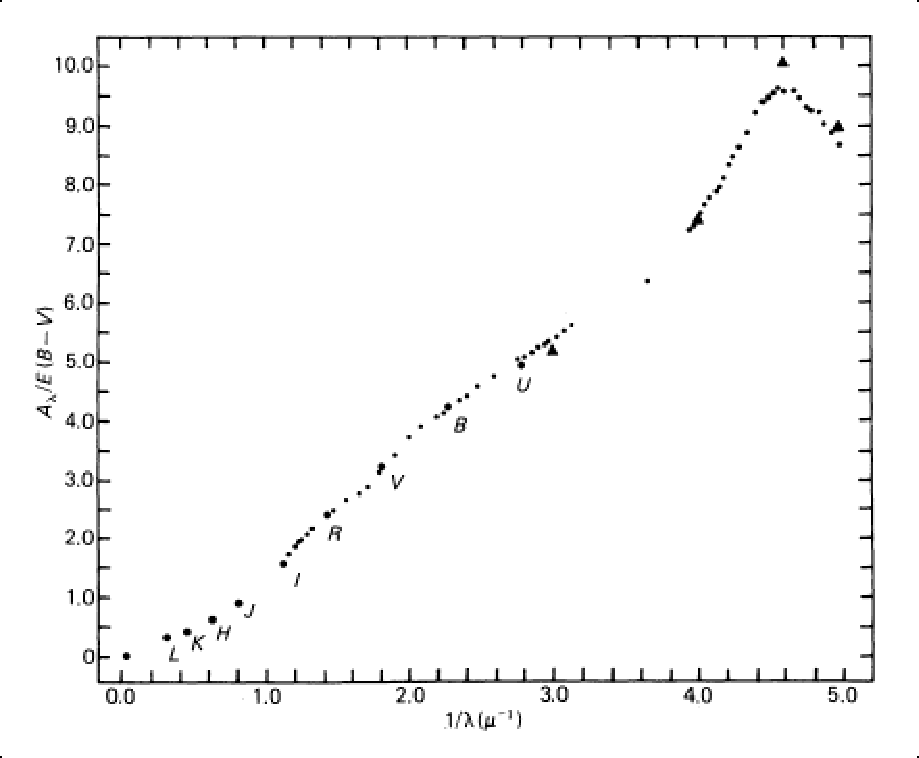
\includegraphics[width=0.5\textwidth]{interstellarreddeningreduite}
  \label{extinction}
  \caption{Variation de $A_V/E_{B-V}$ en fonction de $1/\lambda$}
\end{figure}

\begin{Answer}
  \begin{enumerate}
  \item Calcul de l'extinction
    $$
    E_{B-V} = (A_B- A_V) = (B-V )- (B-V)_0 = 2,25-(-0,25) = 2
    $$
    Le graphique donne $A_V = 3 E_{B-V}$, d'où:
    $$
    A_V =3 \times 2 = 6
    $$
  \item Le graphique donne $A_K = 0.5 \times E_{B-V}$, d'où:
    $$
    A_K = 0.5 \times 2 = 1
    $$
  \item L'extinction est beaucoup plus faible dans l'IR que dans le
    visible.
  \end{enumerate}
\end{Answer}

\section{Galaxies}

\subsection{Classification morphologique des galaxies}

\begin{Exercise}[Propriétés « physiques » de la classification]
  En vous servant du tableau sur les propriétés quantitatives de la
  séquence de Hubble, répondez aux questions suivantes :
  \begin{enumerate}
  \item Que peut-on dire sur la fraction de gaz dans les galaxies
    selon le type morphologique ?
  \item Que peut-on dire de la densité surfacique de masse, en
    supposant que toute la masse des galaxies est concentrée dans un
    disque mince ?
  \end{enumerate}
\end{Exercise}

\begin{Answer}
  \begin{enumerate}
  \item La fraction de masse de gaz est donnée par le rapport de la
    masse de gaz à la masse totale. Ce rapport augmente des S0 aux
    irrégulières.
  \item La densité surfacique de masse est $S = M/ \pi R^2$. Elle
    diminue des S0 aux irrégulières.
  \end{enumerate}

  Dans le tableau ci-dessous, les valeurs de
  $M_{\mathrm{gaz}}/M_{\mathrm{totale}}$ et de $S$ sont obtenues
  statistiquement sur un échantillon de plusieurs milliers de
  galaxies. Ce ne sont donc pas les valeurs obtenues par le calcul
  direct sur les médianes, mais le comportement reste le même.

  \begin{center}
    \begin{tabular}{|c|c|c|c|c|c|c|}
      \hline
      Propriétés & E,SO & S0a,Sa & Sab,Sb & Sbc,Sc & Scd,Sd & Sm,Im \\
      \hline
      $M_{\mathrm{totale}}$ ($10^{10}M_{\odot}$) & & 22.6 & 32.4 & 19.0 & 7.9 &
      1.6 \\
      \hline
      $M_{\mathrm{gaz}}$ ($H$ neutre en $10^{9}M_{\odot}$) & 1.24 & 5.62 &
      15.14 & 15.85 & 9.33 & 2.40\\
      \hline
      $M_{\mathrm{gaz}}/M_{\mathrm{totale}}$ & & 0.03 & 0.05 & 0.08 & 0.11 & 0.15 \\
      \hline
      diamètre (kpc) & 21.1 & 19.8 & 25.1 & 22.4 & 17.7 & 8.5  \\
      \hline
      S ($M_{\odot}/pc^2$) &  & 188.9 & 154.7 & 124.2 & 91.4 & 74.5 \\
      \hline
    \end{tabular}
  \end{center}
\end{Answer}


\begin{Exercise}[de Vaucouleurs et autres classifications]
  Donnez la classification simplifiée (E, S0, SA, SAB, SB) des
  galaxies données dans la partie cours correspondante dans spirale.

  Est-il toujours facile de classifier les galaxies réelles?
\end{Exercise}

\begin{Answer}
  \begin{center}
    \begin{tabular}{|c|c|c|c|}
      \hline
      % \textbf{N° objet} & \textbf{Nom} & \textbf{Réponse} &
      % textbf{Classification complète dite RC3}\\ \hline
      1  & NGC6070    & SA  & SA(s)cd  \\ \hline
      2  & NGC 7424   & SAB & SAB(rs)cd  \\ \hline
      3  & MESSIER 31 & SA  & SA(s)b  \\ \hline
      4  & MESSIER 33 & SA  & SA(s)cd  \\ \hline
      5  & MESSIER 87 & E0 ou E1 & E+0-1 pec* \\ \hline
      6  & NGC 2683   & SA  & SA(rs)b  \\ \hline
      7  & NGC 1300   & SB  & (R')SN(r'1)b  \\ \hline
      8  & NGC 1097   & SB  & (R'\_1:)SB(r'l)b  \\ \hline
      9  & NGC 4321   & SAB & SAB(s)bc \\ \hline
      10 & MESSIER 83 & SAB & SAB(s)c \\ \hline
    \end{tabular}
  \end{center}

  Galaxies lointaines sans noms (11). La classification demandée est
  SB. Ces objets sont considérés comme des galaxies barrées mais n'ont
  pas été précisément classifiées à cause du manque de résolution des
  images (HST Deep Field North).

  *pec: 'peculiar' à cause du jet provenant du noyau actif
\end{Answer}

\subsection{Constituants des galaxies}

\begin{Exercise}[Les étoiles]
  Si l'on considère une sphère de rayon 10 kpc peuplée par $10^{11}$
  étoiles dont le rayon est égal à celui du soleil, calculez la
  fraction de volume occupé par les étoiles.
\end{Exercise}

\begin{Answer}
  La fraction est de $10^{11}\times \left(\frac{0.7\times
      10^{6}}{10\times 3.08\times 10^{16}}\right)^{3}\approx 10^{-20}$
\end{Answer}


\begin{Exercise}[La matière noire]
  Donnez l'expression de l'accélération $a$ centrifuge en fonction de
  $V$, et $R$, la vitesse circulaire d'une étoile à une distance $R$
  du centre de la galaxie.  Écrire la loi de Newton pour cette
  étoile~: l'accélération $a$ en fonction de la masse $M$ incluse dans
  le rayon $R$.  En déduire la loi de décroissance de $V$ en fonction
  du rayon $R$ de l'étoile, en supposant que la masse $M$ reste
  constante (c'est-à-dire que toute la masse de la galaxie est
  comprise dans la sphère de rayon $R$).
\end{Exercise}

\begin{Answer}
  L'accélération centrifuge est donnée simplement par $a = V^2/R$.  La
  loi de Newton nous dit alors que l'accélération de l'étoile est
  proportionnelle à la masse $M$ avec $a = G M/R^2$, où $G$ est la
  constante universelle de la gravitation.  On en déduit alors
  facilement que $V^2/R = GM/R^2$ donc $V^2 \propto M/R$.

  Si $M$ reste constant avec $R$ qui croit, alors $V^2$ doit décroître
  comme $1/R$.
\end{Answer}

\subsection{Exemple de galaxie : la Voie Lactée }

\begin{Exercise}[Morphologie de notre galaxie]
  En examinant en détail l'image de notre galaxie prise par COBE/DIRBE
  (Fig.~\ref{cobe}) on distingue que le bulbe de la Voie Lactée n'est
  pas symétrique.
  \begin{enumerate}
  \item Examiner cette image et essayer de mesurer la hauteur du
    bulbe~; à droite, puis à gauche du centre de la Galaxie
  \item Donner une explication plausible de cette asymétrie, en se
    rappelant notre position très particulière par rapport au centre
    de notre galaxie, et en se rappelant des différentes composantes
    qui composent notre Galaxie.
  \end{enumerate}
\end{Exercise}

\begin{figure}[htp]
  \centering
  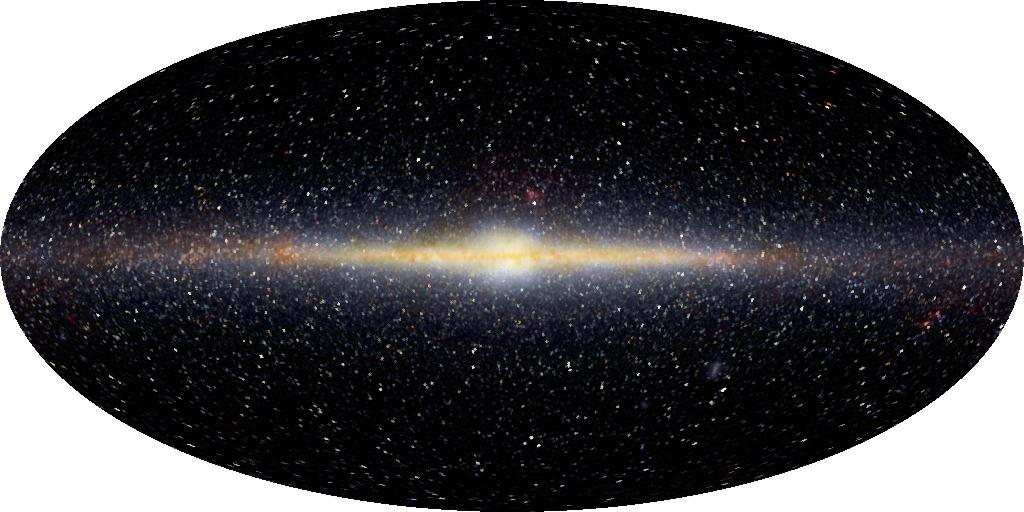
\includegraphics[width=0.8\textwidth]{milky2w}
  \label{cobe}
  \caption{Notre galaxie vue par COBE/DIRBE.}
\end{figure}

\begin{Answer}
  Le bulbe de la galaxie vue en infrarouge est effectivement
  asymétrique:
  \begin{enumerate}
  \item Le coté gauche a une épaisseur légèrement plus grande que le
    coté droit.
  \item Ça n'est pas un effet de populations stellaires, ou
    d'extinction due à la poussière, mais bien une épaisseur
    réellement plus grande d'un coté que de l'autre. Ce que l'on voit
    est en fait un effet de projection : c'est en fait la barre de la
    Galaxie que nous observons. Cette barre étant inclinée à 35 degrés
    environ par rapport à nous, le coté gauche étant proche de nous,
    le coté droit loin de nous (de l'autre coté du centre
    galactique). Une des extrémités de la barre est donc plus proche
    de nous, et par projection elle apparaît plus haute...
  \end{enumerate}
\end{Answer}

\begin{Exercise}[Le centre galactique]
  L'image ci-dessous (Fig.~\ref{centregalac}) montre l'orbite de
  l'étoile ayant la plus grande vitesse autour du centre galactique. À
  partir des données (période en années de 15.2 ans, et demi grand-axe
  de 0.119 arcsecondes) de cette orbite, retrouver l'estimation de la
  masse incluse dans ce rayon au centre de notre Galaxie en utilisant
  la troisième loi de Kepler. On rappelle que nous sommes à environ
  8.5~kpc du centre galactique et que G, la constante
  gravitationnelle, vaut $6,6742.10^{-11} m^3 kg^{-1} sec^{-2}$.  La
  masse visible étant estimée à environ 106 masses solaires, en
  déduire une estimation de la masse noire centrale (le fameux trou
  noir) de notre Galaxie.
\end{Exercise}

\begin{figure}[htp]
  \centering
  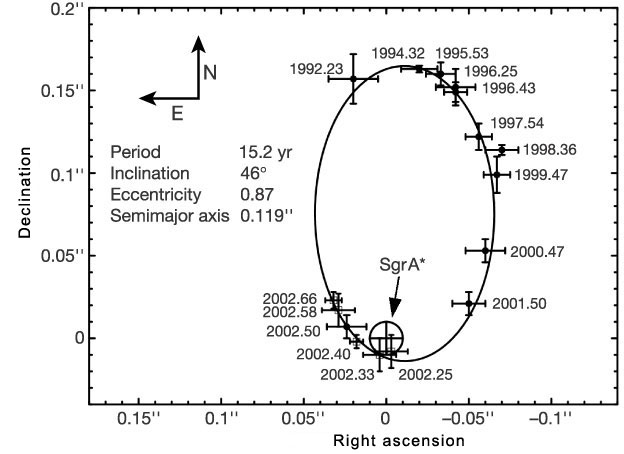
\includegraphics[width=0.5\textwidth]{nature01121-f2_2}
  \label{centregalac}
  \caption{Orbite de l'étoile S2 autour du centre galactique SgrA*
    (Schödel et al. 2002).}
\end{figure}

\begin{Answer}
  On rappelle que G, la constante gravitationnelle, vaut
  $6,6742.10^{-11} m^3kg^{-1}sec^{-2}$

  Nous allons d'abord transformer la taille du demi grand-axe
  d'arcseconde en mètres, et ensuite, la période en secondes:
  \begin{itemize}
  \item 1 arcseconde équivaut à $1/3600$~degrés, donc à $8.5~kpc$ ,
    cela revient à environ $0.041~pc$. Le demi grand axe est donné
    comme étant égal à $0.119$~arcseconde, donc cela équivaut à~:
    $$
    a = 0.119\times0.041 = 0.0048~pc = 0.0048\times 3.08 \times
    10^{16} = 1.5 \times 10^{14}~m
    $$

  \item la période $T$ est donnée de 15.2 ans donc~: $T=479347200~s$
  \end{itemize}

  Enfin la troisième loi de Kepler dit que le rapport $T^2/a^3$ est une
  constante k qui ne dépend que de la masse du système.

  Cette constante k est simplement donnée par : $4\pi^2/(GM)$ donc on
  peut écrire que:
  $$
  M = \frac{4\pi^2 a^3}{T^2 G}
  $$

  En application numérique cela donne (en kg, vérifiez bien que
  l'équation est homogène dans ses unités):
  $$
  M = \frac{ 4 \times \pi^2 \times (1,5 \times 10^{14})^3 } { (479 347
    200)^2 \times 6,6742 \times 10^{11} } = 8,7 \times 10^{36}~kg
  $$
  et ceci exprimé en masses solaires: $M \approx 4,4 \times
  10^6~M_{\odot}$
\end{Answer}

\subsection{Le groupe local}

\begin{Exercise}
  Compter le nombre de galaxies ayant un diamètre plus petit que 6
  kpc, et celles ayant un diamètre plus grand. Quelles sont les
  galaxies qui dominent en nombre ? Et en luminosité totale ?
  (Fig.~\ref{listgalac})
\end{Exercise}

\begin{figure}[htp]
  \centering
  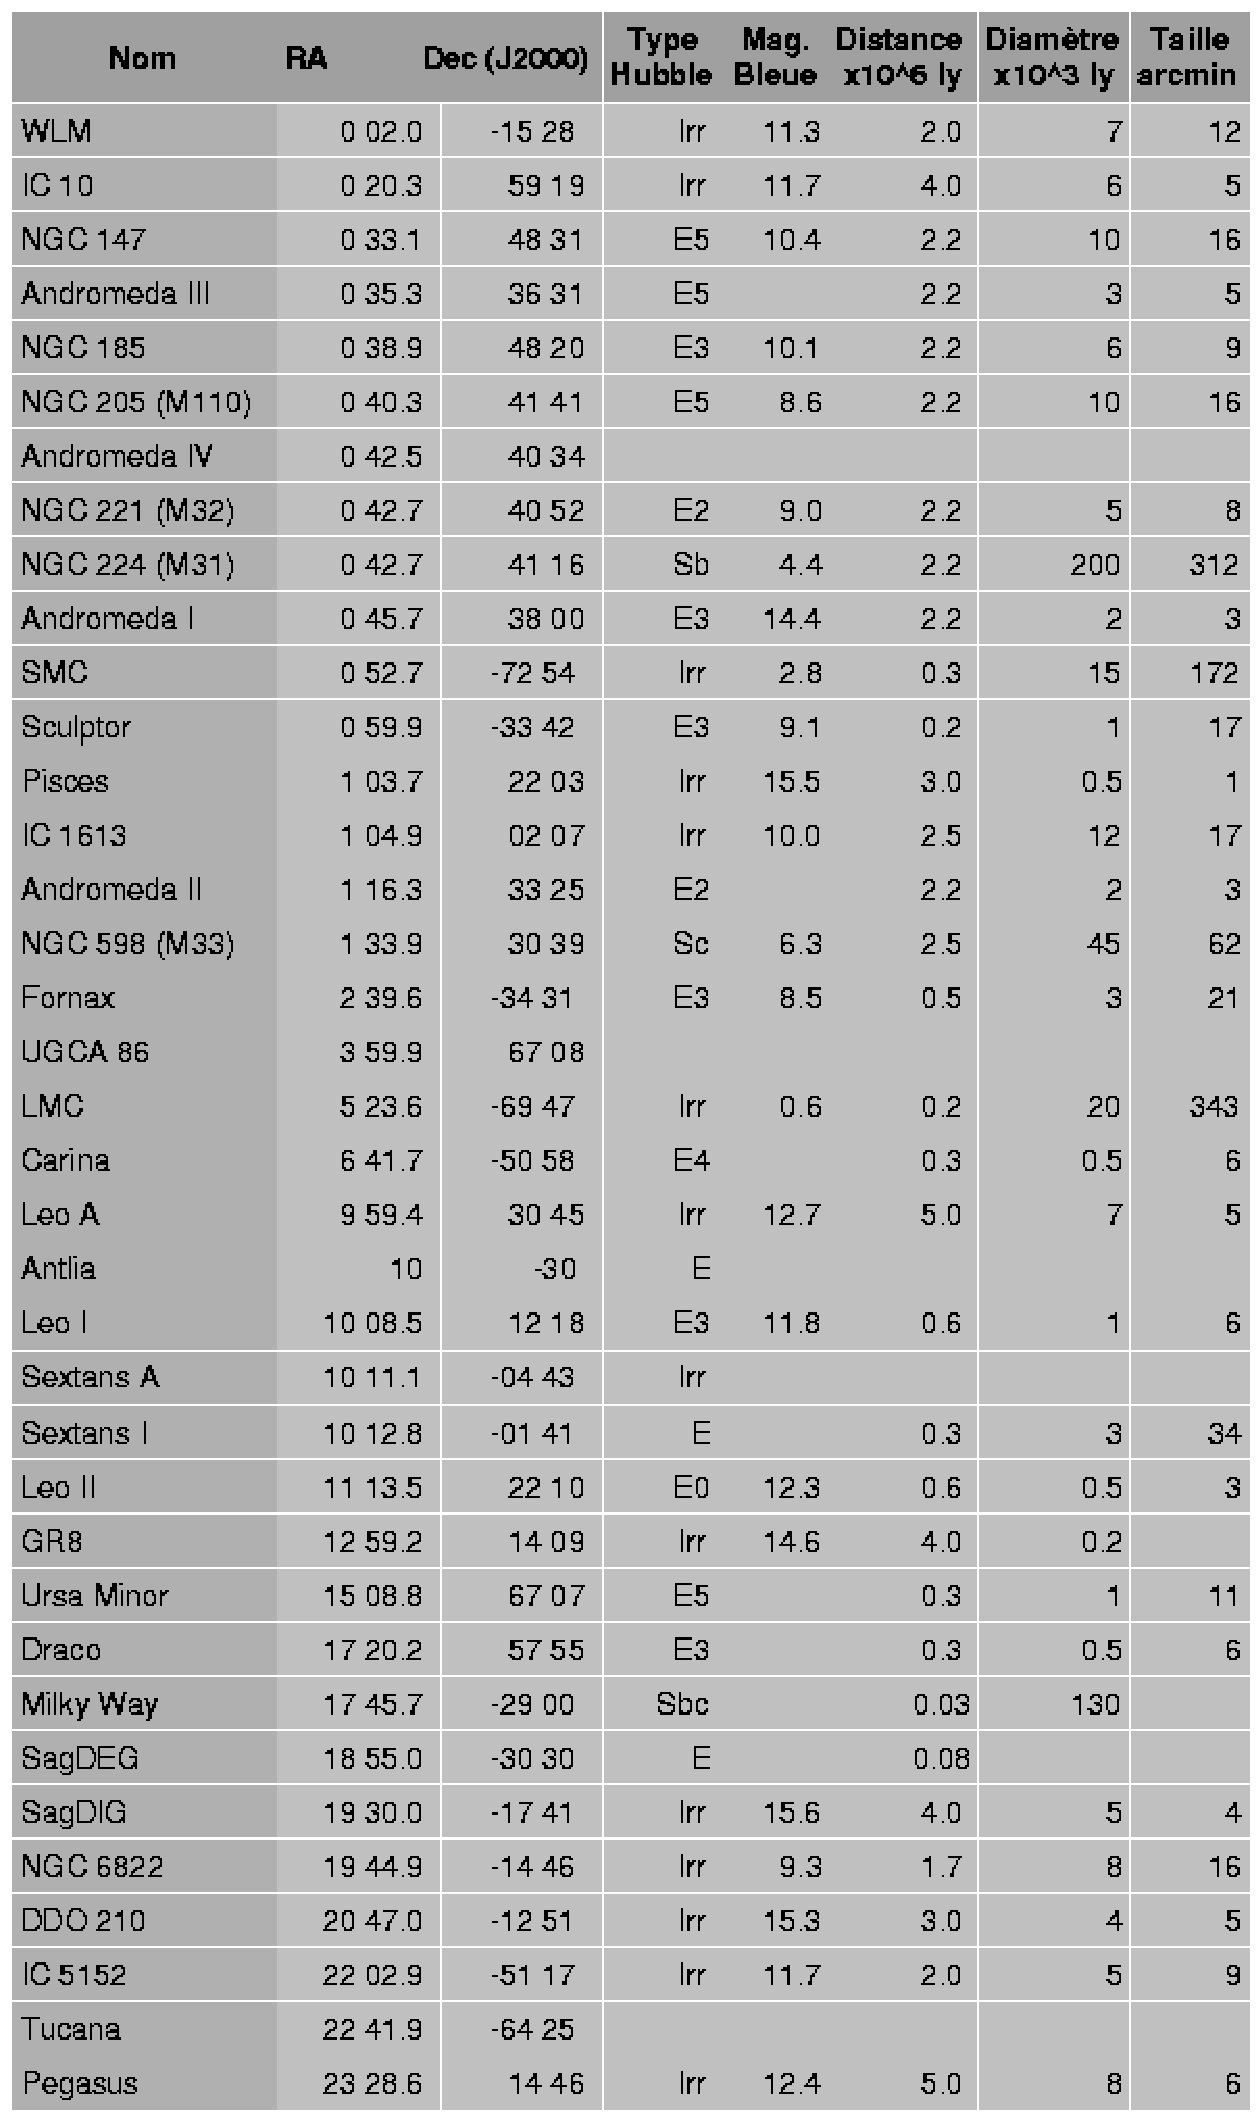
\includegraphics[height=\textheight]{listegalaxiegroupelocal}
  \label{listgalac}
  \caption{Liste des galaxies du Groupe Local, avec leurs noms, leurs
    positions sur le ciel, le type de Hubble, la distance, le diamètre
    en milliers d'années-lumière et en arcminutes sur le ciel.}
\end{figure}

\begin{Answer}
  Il y a 26 petites galaxies -- dites « naines » -- sur les 30
  galaxies dont on nous donne la taille, et seulement 2 galaxies avec
  un diamètre de plus de 30 kpc : M31 et la Voie Lactée). Ce sont donc
  les galaxies naines qui dominent en nombre, mais elles ne dominent
  pas en luminosité totale.
\end{Answer}

\subsection{Distribution des galaxies dans l'univers}

\begin{Exercise}[Fonction de luminosité]
  \begin{enumerate}
  \item Exprimer la loi de Schechter en magnitudes absolues.
  \item Quelle est la signification physique de la loi de Schechter?
  \end{enumerate}
\end{Exercise}

\begin{Answer}
  \begin{enumerate}
  \item En magnitude
    $$
    \Phi (M) = 0.4 \ln (10) \Phi ^{*}10^{0.4(\alpha +1)(M^{*}-M)}\exp
    \left( -10^{0.4(M^{*}-M)} \right)
    $$

  \item Cette fonction empirique montre bien la prédominance des
    galaxies de faible luminosité intrinsèque.
  \end{enumerate}
\end{Answer}

\subsubsection{Effets d'environnement, collisions et fusions}

\begin{Exercise}[Calcul de la fréquence des collisions dans un
  amas]
  On considère un amas de galaxies qui a les caractéristiques
  suivantes:
  \begin{itemize}
  \item il est supposé sphérique, de diamètre $D_{amas}$ en pc
  \item il contient $N_{galaxies}$ identiques et réparties
    uniformément dans l'amas
  \item les galaxies sont supposées animées d'une vitesse uniforme
    $v_{galaxies}$ en km/s
  \end{itemize}

  \begin{enumerate}
  \item Donner l'expression de la densité numérique de galaxies dans
    l'amas en $pc^{-3}$.

  \item On suppose maintenant que les galaxies ont un diamètre typique
    $D_{galaxies}$ (en pc). En modélisant les galaxies comme des
    sphères dures (boules de billard...) de diamètre $D_{galaxies}$,
    donner l'expression de la section efficace $S_{efficace}$ (en
    $pc^2$) lors d'une collision/interaction entre deux galaxies.

  \item Donner l'expression du nombre de collisions/interactions que
    subit une galaxie de l'amas pendant la durée $dt$ (en années). En
    déduire, pour une galaxie, le temps caractéristique de collision
    et le libre parcours moyen.

  \item En déduire le temps entre deux collisions/interactions dans
    l'amas.

  \item Calcul de la fréquence des collisions dans un amas:
    Considérons un amas de $N=850$ galaxies dont le diamètre est
    $D=7~Mpc$ et dont la dispersion des vitesses est $V =
    650~km/s$. Explicitez le calcul numérique du temps moyen entre
    deux collisions pour l'amas considéré.
  \end{enumerate}
\end{Exercise}

\begin{Answer}
  \begin{enumerate}
  \item Le volume de l'amas est
    $$
    V_{amas}=\frac{\pi}{6}D_{amas}^3
    $$
    et la densité numérique de galaxies est donc
    $$
    n_{galaxies}=\frac{N_{galaxies}}{V_{amas}}=
    \frac{6N_{galaxies}}{\pi D_{amas}^3}
    $$
    (en nombre de galaxies par $pc^3$ si le diamètre de l'amas est en
    pc)

  \item Deux galaxies entreront en collision/interaction lorsqu'elle
    passent à une distance < $D_{galaxies}$ l'une de l'autre. La
    section efficace de collision est donc $S_{efficace}=\pi
    D^2_{galaxies}$ en $pc^2$ si le diamètre des galaxies est exprimé
    en $pc$.

  \item Le volume «balayé» par une galaxie pendant le temps dt est le
    suivant:
    $$
    V = \frac{3.15\,10^7 \text{(s par année)}}{%
      3.09\,10^{13} \text{(km par pc)}}
    \times v_{galaxies} \times S_{efficace} \times dt
    $$
    Le nombre de collisions pendant ce temps $dt$ est donc
    $N_{collision} = n_{galaxie}V$. Le temps caractéristique de
    collision/interaction $t_{collision}$ correspond à $dt$ tel que
    $N_{collisions} = 1$. Le libre parcours moyen est $l =
    v_{galaxies} \times t_{collision}$.
    $$
    \tau_{collision} =
    \frac{3.09 \times 10^{13}}{6 \times 3.15 \times 10^7}
    \frac{D^3_{amas}}{D^2_{galaxies} \times v_{galaxies} \times N_{galaxies}}
    $$

  \item Le temps caractéristique de collision/interaction dans l'amas
    est $t_{collision}^{amas} = \tau_{collision}/N_{galaxies}$ (on
    considère ici l'amas entier et non plus une galaxie unique).
  \end{enumerate}

\end{Answer}



\subsection{Équilibre gravitationnel}

\begin{Exercise}[Théorème du Viriel scalaire]
  Le théorème du Viriel peut aussi s'écrire :
  $$
  \frac{2K}{U}=-1
  $$
  Imaginez que vous vouliez construire un système stellaire, en
  donnant à $N$ étoiles leurs positions et leurs vitesses, et où vous
  auriez:
  $$
  \frac{2K}{U}>-1
  $$
  \begin{enumerate}
  \item Comment feriez-vous ? (donner un exemple)
  \item Comment le système évoluerait-il ?
  \end{enumerate}
\end{Exercise}

\begin{Answer}
  \begin{enumerate}
  \item Il suffit de donner une position quelconque aux étoiles mais
    en leur donnant à toute une vitesse nulle. On aurait alors $K=0$,
    et ainsi on aurait bien la condition remplie!

  \item Si cette condition est remplie, c'est que l'énergie cinétique
    est trop faible par rapport à l'énergie potentielle (en valeur
    absolue). Il manque aux étoiles de la vitesse pour que le système
    reste à l'équilibre, et il va donc se réarranger, avec un rayon
    plus petit.
  \end{enumerate}
\end{Answer}

\begin{Exercise}[Application du théorème du Viriel]
  On va maintenant utiliser le théorème du Viriel pour remplir le
  tableau ci-dessous, donnant les rayons, masses et vitesse
  caractéristiques de différents système stellaires.  Veuillez
  compléter ce tableau.  (On prendra $G$ en fonction d'unités
  astronomiques pratiques, ainsi $G=0.004301$
  pc.km$^{2}$.s$^{-2}$.M$_{\odot}^{-1}$)

  \begin{center}
    \begin{tabular}{|c|c|c|c|}
      \hline
      Système & R (pc) & V (km/s) & M ($M_{\odot}$) \\ \hline
      Amas globulaire & 10 & 10 &  \\ \hline
      Galaxie & 50~000 & 200 & \\ \hline
      Amas de galaxies & 1~000~000  & 1000  &  \\ \hline
    \end{tabular}
  \end{center}
\end{Exercise}

\begin{Answer}
  \begin{center}
    \begin{tabular}{|c|c|c|c|}
      \hline
      Système & R (pc) & V (km/s) & M ($M_{\odot}$) \\ \hline
      Amas globulaire & 10 & 10 & $1,4\times 10^6$ \\ \hline
      Galaxie & 50~000 & 200 & $2,3\times 10^{11}$ \\ \hline
      Amas de galaxies & 1~000~000  & 1000  &  $1,4\times 10^{15}$ \\ \hline
    \end{tabular}
  \end{center}
\end{Answer}

\begin{Exercise}[Temps cinématique]
  On va maintenant calculer le temps cinématique $t_c$ pour différents
  systèmes stellaires. Veuillez compléter le tableau ci-dessous.  (Une
  fois de plus, on prendra $G$ en fonction d'unités astronomiques
  pratiques, ainsi $G=0.004301$ pc.km$^{2}$.s$^{-2}$.M$_{\odot}^{-1}$)
  \begin{center}
    \begin{tabular}{|c|c|c|c|}
      \hline
      Système & R (pc) & M ($M_{\odot}$) & $t_c$ (ans) \\ \hline
      Amas ouvert & 1 & 500 &  \\ \hline
      Amas globulaire & 10 & $10^5$ &  \\ \hline
      Galaxie & 50~000 & $10^{12}$ & \\ \hline
    \end{tabular}
  \end{center}
  Que remarquez-vous sur ces temps cinématiques pour les différents
  systèmes ?
\end{Exercise}

\begin{Answer}
  \begin{center}
    \begin{tabular}{|c|c|c|c|}
      \hline
      Système & R (pc) & M ($M_{\odot}$) & $t_c$ (ans) \\ \hline
      Amas ouvert & 1 & 500 & $10^6$ \\ \hline
      Amas globulaire & 10 & $10^5$ & $2\times 10^6$ \\ \hline
      Galaxie & 50~000 & $10^{12}$ & $2\times 10^8$ \\ \hline
    \end{tabular}
  \end{center}

  Les temps cinématiques pour un amas ouvert et un amas globulaire ne
  sont pas vraiment différents malgré leurs tailles respectives très
  différentes.  De même entre une galaxie et un amas globulaire: il ne
  faut qu'environ 100 plus de temps à une étoile avec une vitesse
  typique pour traverser une grosse galaxies qu'un amas globulaire
  (bien sur les vitesses caractéristiques ne sont pas les mêmes pour
  ces 2 systèmes).
\end{Answer}

% ===============================================================================

\chapter{Vie des structures - Cosmologies}

\section{Espace et temps absolus}

\begin{Exercise}[La faiblesse de la force de gravitation]
  Marcel et Naomi ressentent l'un pour l'autre une certaine attirance;
  quelle part en revient tout bêtement à la force de gravitation
  universelle, lorsque leurs centres de gravité respectifs sont
  distants de 1 mètre ?  Quelle masse, au même point de la Terre,
  présente un poids égal à cette force ?  Marcel pèse, à Lyon, 700 N,
  et Naomi 580 N.  Le rayon de la Terre à Lyon sera supposé égal à
  6365~km.  La constante de la gravitation et la masse de la Terre
  sont données dans les annexes du cours...
\end{Exercise}

\begin{Answer}
  Il s'agit, simplement, d'appliquer la formule de Newton deux fois
  pour trouver les masses respectives de Marcel et Naomi, puis une
  troisième fois pour calculer l'attraction qui s'exerce entre eux, en
  prenant garde aux unités.
  $$
  F = G \frac{m_1 m_2}{d^2}
  $$

  On retrouve d'abord les valeurs des constantes : $G = 6,672 \times
  10^{-11}$, $M_{\oplus} = 5,976 \times 10^{24}~kg$, et $R = 6365~km$
  qui est donné dans l'énoncé.

  On écrit donc:
  $$
  P_{\mathrm{Marcel}} = G \frac{M_{\mathrm{Marcel}}M_{\oplus}}{R^2}
  $$
  soit encore:
  $$
  M_{\mathrm{Marcel}} = \frac{P_{\mathrm{Marcel}}R^2}{G M_{\oplus}}
  $$
  et donc
  $$
  M_{\mathrm{Marcel}} = \frac{ 6370000^2 \times 700 }{ 6,672 \times
    10^{-11} \times 5,976 \times 10^{24} } = 71,23~kg
  $$
  Cette valeur s'obtiendrait aussi en utilisant la formule $P =
  M_{\mathrm{Marcel}}\times g$, où $g$ est l'accélération de la
  pesanteur à Lyon. Mais l'énoncé ne précise pas la valeur de $g$ à
  Lyon...

  Pour Naomi, on peut utiliser le fait que
  $M_{\mathrm{Naomi}}/M_{\mathrm{Marcel}} =
  P_{\mathrm{Naomi}}/P_{\mathrm{Marcel}}$, puisque les deux personnes
  sont soumises au même champ de gravité. Et donc:
  $$
  M_{\mathrm{Naomi}} = M_{\mathrm{Marcel}}
  \frac{P_{\mathrm{Naomi}}}{P_{\mathrm{Marcel}}} = 71,23 \times
  \frac{58}{70} = 59,02~kg
  $$
  D'où $F_{\mathrm{Naomi}-\mathrm{Marcel}} = ( 6,672 10^{-11} \times
  71,23 \times 59,02 ) / 1 = 2,8 10^{-7}~N$.

  La masse qui présenterait un poids égal à cette valeur en cet
  endroit serait de : $M = ( 63700002 \times 2,8 10^{-7} ) / ( 6,672
  10^{-11} \times 5,976 10^{24} ) = 2,85 10^{-8} kg = 28,5~\mu g$.

  Elle peut également se calculer, d'après une remarque déjà faite,
  par $M = 71,23 \times 2,8 10^{-7} / 700$. L'attraction
  gravitationnelle est une force \emph{très faible}, c'est même la
  plus faible des quatre forces fondamentales de l'univers...
\end{Answer}

\subsection{Problèmes de l'univers de Newton}

\begin{Exercise}[L'instabilité gravitationnelle]
  Pourquoi Newton pense-t-il que ces trois hypothèses supplémentaires
  permettraient, chacune, de « sauver » l'univers de la catastrophe
  gravitationnelle?
\end{Exercise}

\begin{Answer}
  \begin{itemize}
  \item Si l'univers est infini, tout point est entouré d'une
    distribution de matière à symétrie sphérique, et restera donc
    immobile.
  \item Si l'univers est en expansion, et bien, tant qu'il l'est,
    c'est qu'il n'est pas en train de se contracter !
  \item Si l'univers est très jeune, il n'a pas encore eu le temps de
    démarrer sa contraction gravitationnelle de façon sensible, et
    voilà ...
  \end{itemize}
\end{Answer}

\begin{Exercise}[Le paradoxe d'Olbers]
  En quoi le fait que l'univers soit jeune et en expansion peut-il
  permettre d'expliquer la noirceur du ciel nocturne ?
\end{Exercise}

\begin{Answer}
  \begin{itemize}
  \item Si l'univers est jeune, du fait de la vitesse finie de
    propagation de la lumière, celle qui provient des objets très
    lointains n'a pas eu le temps de nous parvenir.
  \item Si l'univers est en expansion, la lumière qui nous parvient
    des objets très lointains a été affaiblie par cette expansion
    (ceci sera traité plus loin dans le cours), au point de ne pas
    être détectable.
  \end{itemize}
\end{Answer}

\section{La rupture relativiste}

\subsection{Vitesse de la lumière}

\begin{Exercise}[La première mesure de $c$]
  Si Roemer a fait le calcul (ce que l'on ignore, mais cela semble
  assez probable), et en supposant qu'il utilisait la même valeur de
  la distance Terre-Soleil que les astronomes d'aujourd'hui, quelle
  valeur de $c$ a-t-il obtenue?
\end{Exercise}

\begin{Answer}
  Si la lumière met $8+8 = 16$ minutes pour traverser l'orbite de la
  Terre, c'est à dire pour franchir une distance de $2~U.A$., sa
  vitesse est $c = 2 \times 1,49598 \times 10^{11} / ( 16 \times 60 )
  = 3,11 \times 10^8~m~s^{-1}$. Ceci suppose que la valeur de
  l'U.A. admise alors était la même qu'aujourd'hui, ce qui n'est
  certainement pas exact : en 1675, on n'avait pas encore très bien
  mesuré la distance de la Terre au Soleil ... La valeur de deux fois
  huit minutes est elle-même approximative. Roemer aurait plutôt
  trouvé $2 \times 10^8~m~s-1$, dit-on. La première détermination
  sérieuse de l'Unité Astronomique est due à Cassini et Richer, en
  1671. Il faudra attendre le XXe siècle et les méthodes d'écho radar
  pour disposer de mesures très précises de cette valeur.
\end{Answer}

\subsection{Relativité générale}

\subsubsection{Einstein dans l'ascenseur}

\begin{Exercise}[L'équivalence gravité/accélération]
  On dit que, pour la Relativité Générale, gravitation et accélération
  sont équivalentes, mais que cette équivalence n'est que
  locale. C'est à dire qu'aucune expérience de physique ne permet de
  distinguer les effets de l'une de ceux de l'autre, mais seulement
  tant qu'on se limite à un très petit domaine spatial. En gros, c'est
  à peu près vrai dans un dé à coudre, cela ne l'est plus vraiment
  dans un stade de foot...

  En reprenant l'exemple simple de l'ascenseur d'Einstein, pouvez-vous
  montrer qu'en effet il est facile de distinguer pesanteur et
  accélération par la fusée si on abandonne la localité. Il suffit de
  modifier l'ascenseur...
\end{Exercise}

\begin{Answer}
  À grande échelle, le champ de gravité qui environne un corps massif
  reste en général tout à fait discernable d'une accélération
  constante.  Par exemple, dans l'image de l'ascenseur utilisée dans
  le cours, il ne faut pas que la cabine soit trop étendue. Sinon, le
  parallélisme ou le non-parallélisme des actions sur des masses très
  éloignées l'une de l'autre trahirait la « vraie » nature du champ.
  La cabine de gauche, supposée à grande distance de la planète, et
  accélérée vers le haut (flèche bleue), produit des actions
  parallèles (flèches rouges) sur les deux masses-test. La cabine de
  droite, immobile dans le champ de gravitation de la Terre, montre
  des actions convergentes vers le centre de la Terre (flèches
  vertes). Rusés comme ils le sont parfois, les physiciens de
  l'ascenseur finiraient par s'en apercevoir... (Fig.~\ref{grav})

  \begin{figure}[htp]
    \centering
    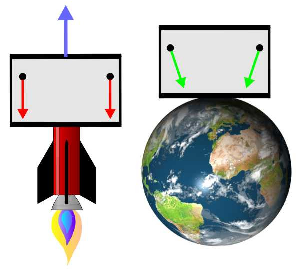
\includegraphics[width=0.4\textwidth]{grav}
    \caption{}
    \label{grav}
  \end{figure}
\end{Answer}

\subsection{Les tests}

\begin{Exercise}[Le décalage gravitationnel vers le rouge]
  Une lampe spectrale émettant la raie Hydrogène Alpha (de longueur
  d'onde en laboratoire 656,3 nm) est utilisée pour communiquer à
  partir d'une capsule en orbite serrée autour d'une étoile à
  neutrons. Le rayon de l'orbite est de 1000 km, la masse de l'étoile
  de 1,5 masses solaires.  À quelle longueur d'onde le vaisseau qui a
  lancé la capsule, et se tient prudemment à grande distance, doit-il
  rechercher les signaux?
\end{Exercise}

\begin{Answer}
  Le décalage gravitationnel subi à la distance r d'un corps de masse
  M s'écrit:
  $$
  z = \frac{GM}{c^2r}
  $$
  Et donc:
  $$
  z = \frac{ 6,672 \times 10^{-11} \times 1,5 \times 1,989 \times
    10^{30} }{ 2997924582 \times 10^6 } = 2,215 \times 10^{-3}
  $$
  Mais:
  $$
  z = \frac{ \delta \lambda } { \lambda_0 }
  $$
  Et donc:
  $$
  \lambda = \lambda_0 + \delta \lambda = (1+z)\lambda_0
  $$
  D'où le $\lambda$ cherché: $\lambda = 1,00221 \times 656,3 =
  657,75~nm$.
\end{Answer}

\section{Le big bang}

\subsection{Expansion de l'univers...}

\begin{Exercise}[...limitée par $c$?]
  Plus une galaxie est éloignée de notre Voie Lactée, plus les
  astronomes lui trouvent une vitesse d'éloignement élevée. C'est
  l'expansion de l'univers. Mais, quand la distance croît sans cesse,
  elle atteint un moment une valeur $d_c$ telle que :
  $$
  V = H_0 d_c > c
  $$
  Invraisemblable, n'est-ce pas ?
\end{Exercise}

\begin{Answer}
  Il est interdit par la Relativité Générale de mesurer une vitesse
  égale ou supérieure à $c$ pour un objet de masse non nulle, comme
  une galaxie. Alors ?

  Alors, cela ne pose aucun problème pour l'expansion de l'univers, où
  les objets (les galaxies...) sont immobiles dans un espace dont la
  géométrie s'étire. Les galaxies très lointaines voient effectivement
  leur vitesse apparente atteindre celle de la lumière, et
  disparaissent alors de l'univers observable. Ceci n'enlève rien au
  fait qu'elles continuent à s'éloigner de nous à des vitesses
  supérieures à $c$.

  Signalons que nos moyens d'observation actuels sont loin de nous
  permettre d'observer les objets qui flirtent avec cette limite...
\end{Answer}

\begin{Exercise}[...la même partout?]
  La radiogalaxie 3C 171 (nommée ainsi parce qu'elle occupe la 171e
  position dans le troisième catalogue de radiources établi par
  l'observatoire de Cambridge...) est relativement lointaine;
  entraînée par l'expansion de l'univers, elle présente une vitesse de
  fuite de 63000 km par seconde.

  Montrer que malgré cela, l'astronome Xhbrr'ffttk, qui a là-bas
  découvert l'expansion de l'univers, comme Hubble l'a fait pour nous,
  a lui aussi trouvé une loi qui s'écrit :
  $$
  V_0 = X_0 d_{0^{'}} \quad\text{avec}\quad X_0 = H_0
  $$
  $V_0$ étant la vitesse mesurée à partir de 3C171 pour une galaxie
  lointaine située à la distance $d_0$ de 3C171, et $X_0$ étant bien
  entendu la constante de Xhbrr'ffttk.

  Ainsi, d'une planète de 3C171, comme de la Terre, on observe la même
  expansion universelle, avec la même géométrie, et le même taux...
\end{Exercise}

\begin{Answer}
  Désignons par $V_T$ et $d_T$ les vitesses et distances mesurées à
  partir de la Terre, $V_{3C}$ et $d_{3C}$ celles mesurées à partir de
  3C171.  La vitesse de récession de 3C171 mesurée de la Terre est
  donc $v_T(3C171) = 63000~km/s$.

  Considérons une autre galaxie, G, observée à la fois de la Terre et
  de 3C171. On peut écrire :
  \begin{eqnarray*}
    \vec{V}_{3C}(G) &=& \vec{V}_{3G}(T) + \vec{V}_{T}(G) \\
    &=& -\vec{V}_{T}(3C171) + \vec{V}_{T}(G) \\
    &=& -H_0\vec{d}_{T}(3C171) + H_0\vec{d}_{T}(G) \\
    &=& H_0 \left[ \vec{d}_{T}(G) - \vec{d}_{T}(3C171) \right ] \\
    &=& H_0 \vec{d}_{3C}(G)
  \end{eqnarray*}
  et donc, à partir de 3C171 comme de la Terre, toute les galaxie
  observée semble s'enfuir avec une vitesse proportionnelle à sa
  distance, et le facteur de proportionnalité (la constante de
  Xhbrr'ffttk) est universel : $X_0=H_0$... (Fig.~\ref{H0})

  \begin{figure}[htp]
    \centering
    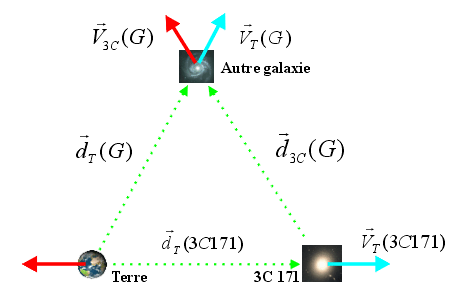
\includegraphics[width=0.4\textwidth]{351922_281}
    \caption{}
    \label{H0}
  \end{figure}
\end{Answer}

\begin{Exercise}[Le facteur d'expansion de l'espace]
  Donner $H_0$ en kilomètres par seconde et par mégaparsec est
  pratique pour les astronomes, mais ne parle guère à l'imagination.
  Passons donc dans des unités plus gouleyantes : si l'on suppose que
  $H_0 = 65 km s^{-1} Mpc^{-1}$, quelle est la valeur de
  l'accroissement annuel d'un kilomètre ? Des mètres ? Des millimètres
  ? Encore moins ?  Beaucoup plus?
\end{Exercise}

\begin{Answer}
  Un mégaparsec (Mpc) vaut $10^6$ parsecs, soit $3.26 10^6$
  années-lumière, soit $3,08 10^{19}~km$... Ceci nous montre que
  $65~km~s^{-1}~Mpc^{-1}$ équivalent à $2,10
  10^{18}~km~s^{-1}~km^{-1}$, ou encore $6,65
  10^{-11}~km~an^{-1}~km^{-1}$. Ce qui signifie que chaque kilomètre
  de l'espace, loin de toute galaxie, s'étire chaque année de $6,65
  10^{-11}~km$, soit environ 67 nanomètres! C'est infiniment dérisoire
  sur un kilomètre, mais sur les distances cosmiques l'effet est
  cumulatif, et cela donne des vitesses qui peuvent être très
  importantes, facilement de l'ordre de celle de la lumière...
\end{Answer}

\subsection{Facteur d'échelle}

\begin{Exercise}[Redshift et facteur d'échelle]
  La radiogalaxie 4C41.17 montre une raie spectrale intense à
  583,2~nm.  Cette raie est identifiée comme la raie Lyman alpha de
  l'hydrogène. En laboratoire, sur la Terre, la longueur d'onde de
  cette raie est de 121,5~nm. Quel était le facteur d'échelle de
  l'univers à l'époque où les atomes d'hydrogène de 4C41.17 émettaient
  cette raie ?
\end{Exercise}

\begin{Answer}
  Il suffit de se souvenir de la relation:
  $$
  1 + z = \frac{\lambda_\text{observé}}{\lambda_\text{émis}} =
  \frac{R_0}{R_\text{émission}}
  $$
  pour trouver $R_{em} = R_0 \times \lambda_{em}/\lambda_0 =
  \lambda_{em}/\lambda_{0}$. Et donc $R_{em} = 121,5/583,2 = 0,208$.
  À l'époque où 4C41.17 émettait la lumière qui nous parvient
  aujourd'hui, l'univers était cinq fois moins « étiré »
  qu'aujourd'hui... Remarquez bien qu'on évite de dire qu'il était
  moins « étendu » : cette expression sous-entendrait des choses sur
  la « taille globale » de l'univers, ce que tout cosmologiste
  raisonnable évite soigneusement de faire, vu son ignorance.
\end{Answer}

\begin{Exercise}[Facteur d'échelle et époque]
  À quelle époque $t_{em}$ la radiogalaxie 4C41.17 de l'exercice
  précédent a-t-elle émis la lumière que nous recevons aujourd'hui à
  $t_0$? On prendra $t_0 = 13.5$ milliards d'années.
\end{Exercise}

\begin{Answer}
  Il suffit de se souvenir de la relation liant le facteur d'échelle
  et le temps cosmologique :
  $$
  R(t)/R_{0} = \left(\frac{t}{t_0}\right)^{2/3}
  $$
  pour trouver $t_{em} = t_0 \times
  \left(R(t_{em})/R_{0}\right)^{3/2}$, et donc $t_{em} = 13,5 \times
  (0,208)^{1,5} = 1,3$~Gan.  4C41.17 émettait la lumière qui nous
  parvient aujourd'hui alors l'univers était âgé d'environ 1,3
  milliards d'années. Environ, car l'équation de départ n'est qu'une
  approximation.
\end{Answer}

\begin{Exercise}[Redshift cosmologique]
  Quel est le redshift de la radiogalaxie 4C41.17 citée dans
  l'exercice précédent?
\end{Exercise}

\begin{Answer}
  On reprend la relation:
  $$
  1 + z = \frac{\lambda_\text{observé}}{\lambda_\text{émis}} =
  \frac{R_0}{R_\text{émission}}
  $$
  pour trouver $1 + z = 1 / 0,208 = 4,807$, et donc $z = 3,807$.
\end{Answer}

\subsection{Film des débuts}

\begin{Exercise}[Nucléosynthèse primordiale ou non?]
  Les éléments légers $\mathrm{H}$, ${}^{2}\mathrm{H}$,
  ${}^{3}\mathrm{H}$, ${}^{4}\mathrm{He}$, ${}^{7}\mathrm{Li}$ sont
  nés avec le Big Bang. Mais d'où proviennent tous les autres éléments
  « lourds », ceux qui entrent dans la composition des objets du
  quotidien ?
\end{Exercise}

\begin{Answer}
  Les chapitres traitant des modèles stellaires et de l'évolution
  stellaire nous fournissent la réponse :
  \begin{itemize}
  \item Jusqu'au ${}^{56}\mathrm{Fe}$, les noyaux sont produits par
    les étoiles.  La source d'énergie de celles-ci est d'origine
    thermonucléaire, et elles sont des usines à fabriquer, par fusion,
    des noyaux lourds à partir de noyaux plus légers.
  \item Au-delà, seules les explosions de supernovae atteignent des
    températures suffisantes (plusieurs $10^9~K$) pour pouvoir
    synthétiser les noyaux très lourds, jusqu'aux éléments
    transuraniens.
  \item Quelques noyaux particuliers (${}^{6}\mathrm{Li}$,
    ${}^{9}\mathrm{Be}$, ${}^{10}\mathrm{B}$) sont sans doute formés
    lors des collisions des rayons cosmiques avec la matière
    interstellaire.
  \end{itemize}
\end{Answer}


\section{Questions diverses}

\subsection{Âge de l'univers}

\begin{Exercise}[Calcul du temps de Hubble]
  La valeur la plus probable, aujourd'hui, de la constante de Hubble
  est $H_0 = 65\;\u{km s^{-1} Mpc^{-1}}$ Quelle conclusion
  pouvez-vous en tirer sur l'âge réel de l'univers?
\end{Exercise}

\begin{Answer}
  Le temps de Hubble est défini par: $1/t_{H0} = H_0 =
  65~\u{km~s^{-1}~Mpc^{-1}}$. Il reste simplement à convertir les
  Mpc (megaparsecs) en kilomètres, et il vient : $1/t_{H0} =
  65~\u{km~s^{-1}} [3,26 10^{19}~\u{km}]^{-1} = 20 \times
  10^{-19}$~s, d'où $t = 5 \times 10^{17}~s = 16 \times
  10^9$~années. On peut donc penser que l'univers est âgé de moins de
  16~milliards d'années.
\end{Answer}

\begin{Exercise}[Age de l'univers et temps de Hubble]
  En partant de la définition de $H_0$ et de la relation trouvée dans
  la section précédente entre le facteur d'échelle $R$ et l'âge $t$ de
  l'univers dans le cas de la densité critique, trouver la relation
  entre $H$ et $t$.
\end{Exercise}

\begin{Answer}
  Par définition:
  $$
  v = H_0.d \quad\text{donc}\quad
  H_0 = \frac{v}{d} = \frac{\d d}{\d t} \frac{1}{d} =
  \frac{\d\left(\epsilon R \right)}{\d t}\frac{1}{\epsilon R}
  \hfill
  $$
  car toute distance, à un instant t, s'écrit:
  $$
  d = \epsilon R(t)
  $$
  où $\epsilon$ est une constante; Et donc:
  \begin{eqnarray*}
    H_0 &=& \frac{1}{R}\frac{\d R}{\d t} \\
    &=& \left ( \frac{t}{t_0} \right )^{-2/3} \times
    \frac{\d\left( \frac{t}{t_0} \right )^{2/3}}{\d t} \\
    &=& \left ( \frac{t}{t_0} \right )^{-2/3} \times
    \left( \frac{t}{t_0} \right)^{-1/3} \frac{2}{3} \frac{1}{t_0} \\
    &=& \left( \frac{t}{t_0} \right)^{-1} \times \frac{2}{3t_0} \\
    &=& \frac{2}{3t}
  \end{eqnarray*}
  Dans le cas critique (univers marginalement ouvert), l'âge de
  l'univers est égal aux deux-tiers du temps de Hubble.
\end{Answer}

\subsection{Distance de l'horizon}

\begin{Exercise}[{Temps de vol, distance, et expansion...}]
  Il y a dix milliards d'années, ce photon que nous recevons
  aujourd'hui a quitté une lointaine galaxie.
  \begin{enumerate}
  \item Cette galaxie se trouvait-elle à dix milliards
    d'années-lumière de nous au moment de l'émission ?
  \item Cette galaxie se trouve-t-elle aujourd'hui à dix milliards
    d'années-lumière de nous ?
  \end{enumerate}
\end{Exercise}

\begin{Answer}
  \begin{itemize}
  \item Le photon a voyagé pendant dix milliards d'années en luttant
    contre l'expansion de l'espace qui contrariait son mouvement; tout
    se passe comme s'il avait parcouru à la vitesse $c$ une distance
    supérieure à celle qui séparait la galaxie de nous au moment de
    l'émission.  Au moment de l'émission, la galaxie était donc à
    moins de dix milliards d'années-lumière de nous.
  \item Depuis que le photon a quitté la galaxie, celle-ci, entraînée
    par l'expansion, a continué à s'éloigner de nous. Le photon a bien
    parcouru (de son point de vue, en admettant qu'il en ait un) dix
    milliards d'années-lumière, puisque sa vitesse par rapport à
    l'espace est à tout instant égale à $c$, mais la galaxie a
    continué sa route pendant tout ce temps, et se trouve aujourd'hui
    à plus de dix milliards d'années-lumière de nous...
  \end{itemize}
\end{Answer}


% ==============================================================================

\chapter{Retour sur Terre - Nos repères dans le ciel}

\section{Se positionner dans le ciel}

\begin{Exercise}[Repérage]
  \begin{enumerate}
  \item Quelles sont les coordonnées horizontales des quatre points
    cardinaux?

  \item Peut-on définir les coordonnées horizontales pour un
    observateur installé au pôle Nord géographique ou au pôle Sud?

  \item Pour quelles valeurs de la hauteur et de la distance zénithale
    un astre est-il visible, c'est-à-dire au dessus de l'horizon?
  \end{enumerate}
\end{Exercise}

\begin{Answer}
  \begin{enumerate}
  \item Les points cardinaux étant par définition sur l'horizon, leurs
    hauteurs sont nulles. Les directions Est-Ouest et Nord-Sud étant
    orthogonales, on a à partir de l'origine la direction Sud
    (Fig.~\ref{position}):
    \begin{center}
      \begin{tabular}{|c|c|c|}
        \hline
        Points cardinaux & Azimut (degrés) & hauteur (degrés) \\ \hline
        Nord & 180 & 0 \\ \hline
        Est & 270 & 0 \\ \hline
        Sud & 0 & 0 \\ \hline
        Ouest & 90 & 0 \\ \hline
      \end{tabular}
    \end{center}
    Remarque: L'azimut des marins est décalé de 180 degrés par rapport
    à celui des astronomes. L'origine des azimuts est le Nord.

  \item Seule la hauteur d'un astre au-dessus de l'horizon peut être
    définie. L'azimut ne l'est pas, la ligne Nord-Sud ou le plan
    méridien étant indéterminé. La verticale du lieu est confondue
    avec l'axe de rotation de la Terre et tout plan passant par la
    verticale du pôle répond à la définition du plan méridien.

  \item Un astre n'est visible que s'il est au-dessus de l'horizon. Sa
    hauteur doit être positive par définition. Sa distance zénithale
    ($90\deg - h$) par conséquent est plus petite que 90~degrés.  Un
    astre sous l'horizon a sa distance zénithale plus grande que
    $90\deg$ (Fig.~\ref{position2}).
  \end{enumerate}

  \begin{figure}[htp]
    \begin{center}
      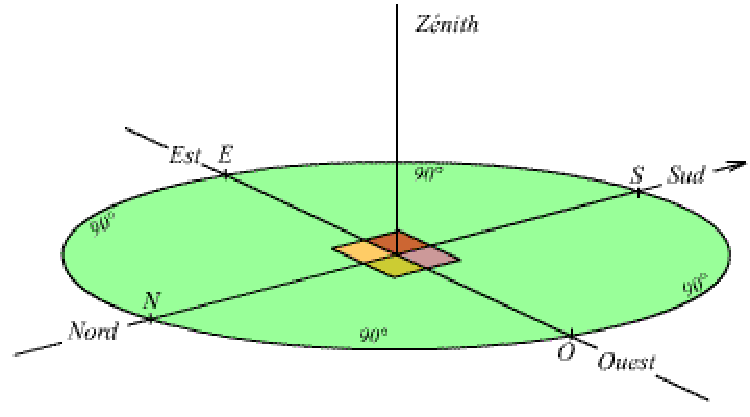
\includegraphics[width=0.4\textwidth]{position}
      \includegraphics[width=0.4\textwidth]{position2}
    \end{center}
    \label{position}
    \label{position2}
    \caption{G.: Points cardinaux. Dr.: Horizon et distance zénithale.}
  \end{figure}
\end{Answer}

\section{Mouvement diurne}

\begin{Exercise}
  \begin{enumerate}
  \item Dans quelle direction se trouve un astre au moment de sa
    culmination en un lieu de latitude $+50\deg$?
  \item Même question pour un lieu situé à l'équateur.
  \item La hauteur d'un astre varie-t-elle au cours du mouvement
    diurne au pôle Nord?
  \end{enumerate}
\end{Exercise}

\begin{Answer}
  \begin{enumerate}
  \item Lors du mouvement diurne, la culmination d'un astre se produit
    lorsque sa hauteur est maximale.  Suivant sa position de l'objet
    sur la sphère céleste (donc sa déclinaison), l'astre passera entre
    le zénith et le pôle (Nord pour un habitant de l'hémisphère nord
    et Sud pour ...) soit entre le zénith et l'horizon opposé au pôle
    visible. À la latitude de $50\deg$, les étoiles dont la
    déclinaison est plus petite que la latitude, la culmination se
    fera du côté Sud de l'observateur.  Pour les autres étoiles, la
    culmination sera du côté Nord (Fig.~\ref{mouvementdiurne2})

    \begin{figure}[htp]
      \centering
      \includegraphics[width=0.3\textwidth]{mouvement_diurne2}
      \includegraphics[width=0.3\textwidth]{mouvement_diurne3}
      \includegraphics[width=0.3\textwidth]{mouvement_diurne4}
      \label{mouvementdiurne2}
      \label{mouvementdiurne3}
      \label{mouvementdiurne4}
      \caption{Mouvement diurne à une latitude $\phi\sim 50\deg$
        (à g.), à l'équateur ($\phi = 0$, au c.) et au pôle nord
        ($\phi = 90\deg$, à dr.).}
    \end{figure}

  \item L'équateur passant par le zénith, toutes les étoiles de
    déclinaisons positives culminent au Nord et les étoiles de
    déclinaisons négatives au Sud. Les étoiles de déclinaisons nulles
    passent au zénith (Fig.~\ref{mouvementdiurne3}).

  \item La verticale étant confondue avec l'axe du pôle, et l'horizon
    avec l'équateur, la déclinaison est égale à la hauteur de l'astre
    qui reste constante lors de la rotation diurne.  Seuls les objets
    de déclinaisons positives sont visibles. C'est pourquoi le Soleil
    dans son mouvement apparent durant l'année donne 6 mois
    consécutifs de jour et 6 mois consécutifs de nuit
    (Fig.~\ref{mouvementdiurne4}).
  \end{enumerate}
\end{Answer}

\begin{Exercise}[Mouvement diurne des étoiles]
  \begin{enumerate}
  \item Comment varie l'azimut d'un astre au cours du mouvement
    diurne, en un lieu de latitude $50\deg$ ? Et aussi $-50\deg$ de
    latitude. Sur la Fig.~\ref{mouvementdiurne}, on a représenté la
    situation en un lieu de l'hémisphère Sud (latitude = $-50\deg$) ;
    $P$ est alors en-dessous de l'horizon et $P'$ est au-dessus.

    \begin{figure}[htp]
      \centering
      \includegraphics[width=0.5\textwidth]{mouvement_diurne}
      \label{mouvementdiurne}
      \caption{Rotation d'une étoile vue de l'hémisphère sud (latitude =
        $-50\deg$).}
    \end{figure}

  \item Les astres se lèvent-ils du côté de l'Est et se couchent-ils
    du côté de l'Ouest aussi bien dans l'hémisphère Nord que dans
    l'hémisphère Sud?
  \item Dans quelle direction géographique un astre culmine-t-il en un
    lieu de latitude $-50\deg$ ?
  \item Le mouvement diurne est-il observé dans le même sens pour un
    observateur de l'hémisphère Nord ou un observateur de l'hémisphère
    Sud?
  \end{enumerate}
\end{Exercise}

\begin{Answer}
  \begin{enumerate}
  \item
    \begin{description}
    \item[Observateur de l'hémisphère Nord (latitude $+50\deg$)] On
      n'envisagera que le cas des étoiles visibles par l'observateur,
      c'est-à-dire celles dont $\delta > -(\pi/2 - \phi)$. Deux
      critères sont a envisager :
      \begin{itemize}
      \item l'étoile a une déclinaison plus grande que la latitude
        $\delta>\phi$ ou $\delta<\phi$
      \item l'étoile est circumpolaire $\delta > \pi/2 - \phi$
      \end{itemize}
      Par la première condition, si $\delta<\phi$, l'azimut de
      l'étoile varie de 0 à $360\deg$, sinon, son azimut oscille
      entre une valeur comprise $\alpha$ entre 90 et $180\deg$
      suivant sa position au passage au méridien et
      $360\deg-\alpha$. L'étoile oscille donc entre $\alpha$,
      $180\deg$ et $360\deg-\alpha$.

      Le deuxième critère (circumpolarité) indique si l'étoile a un
      lever ou un coucher, son azimut varie alors entre les positions
      des levers et couchers et celles définies par le premier
      critère.

      L'observateur orienté vers le Nord voit tourner les étoiles dans
      le sens direct autour du pôle Nord.

    \item[Observateur de l'hémisphère Sud (latitude $-50\deg$)] Les
      mêmes critères s'appliquent pour les limitations des azimuts et
      des levers et couchers, à la différence que l'azimut va osciller
      autour de la valeur $0\deg$ et que regardant le pôle Sud, il
      verra tourner les étoiles dans le sens rétrograde
      (Fig.\ref{mouvementdiurne}).
    \end{description}
  \item Oui. Que l'on soit dans l'hémisphère Nord ou Sud, le sens de
    rotation de la Terre est le même. Les objets apparaissent à l'Est
    et se couchent à l'Ouest.

  \item Au Nord si sa déclinaison est plus grande que la latitude,
    autrement au Sud (Voir exercice 1 du même chapitre).

  \item Non (Voir exercice 4 du chapitre II).
  \end{enumerate}
\end{Answer}

\begin{Exercise}[Coordonnées horaires d'un astre]
  \begin{enumerate}
  \item Quelle est la relation entre la déclinaison et la distance
    polaire?
  \item Quelles sont les coordonnées horaires des quatre points
    cardinaux en un lieu de latitude $\phi$?
  \item Que vaut la déclinaison du zénith en fonction de la latitude
    du lieu?
  \end{enumerate}
\end{Exercise}

\begin{Answer}
  \begin{enumerate}
  \item Comme son nom l'indique, la distance polaire est l'angle entre
    la direction du pôle nord et la direction de l'objet, donc
    $p=90\deg-\delta$

  \item Table~\ref{tbl:coordonnees_horaire} et
    Fig.~\ref{coordonneeshoraire}

    \begin{center}
      \begin{tabular}{|c|c|c|}
        \hline
        Points cardinaux & Angle horaire & Déclinaison \\ \hline
        Sud   & 0h  & -(90 - $\phi$) \\ \hline
        Ouest & 6h  & 0 degré \\ \hline
        Nord  & 12h & 90 - $\phi$ \\ \hline
        Est   & 18h & 0 degré \\ \hline
      \end{tabular}
      \label{tbl:coordonnees_horaire}
    \end{center}

    \begin{figure}[htp]
      \centering
      \includegraphics[width=0.45\textwidth]{coordonnees_horaire}
      \includegraphics[width=0.45\textwidth]{coordonnees_horaire2}
      \label{coordonneeshoraire}
      \label{coordonneeshoraire2}
      \caption{Coordonnées horaires des points cardinaux (à g.) et du
        zénith (à dr.).}
    \end{figure}

  \item La déclinaison du zénith vaut la latitude (positive pour
    l'hémisphère Nord et négative pour l'hémisphère Sud), cf. Fig.
    \ref{coordonneeshoraire2}.
  \end{enumerate}
\end{Answer}

\begin{Exercise}[Coordonnées équatoriales]
  \begin{enumerate}
  \item Une étoile traverse le méridien sud à une hauteur de
    $85\deg$, et le méridien nord à $45\deg$. Trouver la
    déclinaison de l'étoile et la latitude de l'observateur.
  \item Où ces affirmations sont-elles vraies?
    \begin{enumerate}
    \item Castor ($\alpha$-Gem, déclinaison $+31\deg54'$) est
      circumpolaire.
    \item Bételgeuse ($\alpha$-Ori, $7\deg24'$) culmine au
      zénith.
    \item $\alpha$-Cen ($-60\deg46'$) s'élève à une hauteur de
      $20\deg$ au méridien.
    \end{enumerate}
  \end{enumerate}
\end{Exercise}

\begin{Answer}
  \begin{enumerate}
  \item L'étoile tournant autour de la direction du pôle, les deux
    directions $OA$ et $OB$ des passages supérieur et inférieur, sont
    symétriques par rapport à l'axe $OP$. L'angle $\alpha$ égale
    l'angle $\beta$ et
    $$
    \alpha + \beta+180\deg - 45\deg -85\deg = 50\deg
    \quad\to\quad
    \alpha=\beta=25\deg
    $$
    $\alpha$ et $\beta$ sont tous deux les compléments de la
    déclinaison de l'étoile:
    $$
    \beta+\delta = 90\deg
    \quad\to\quad
    \delta=65\deg
    $$
    On calcule la latitude qui vaut la hauteur du pôle au dessus de
    l'horizon: $\phi=\alpha+45\deg=70\deg$.

    \begin{figure}[htp]
      \centering
      \includegraphics[width=0.5\textwidth]{coordonnees_horaire3}
      \label{coordonneeshoraire3}
      \caption{Coordonnées horaires.}
    \end{figure}

  \item
    \begin{description}
    \item[Castor (Gem, $\delta = +31\deg56'$) circumpolaire]
      L'étoile sera juste circumpolaire, c'est-à-dire passera tangent
      à l'horizon Nord, si sa déclinaison est le complément de la
      latitude.  Pour toute latitude plus grande, l'étoile sera plus
      élevée sur l'horizon et ne disparaîtra pas derrière celui-ci
      (Fig \ref{castor}): $\phi>=90\deg-\delta$
      \begin{figure}[htp]
        \centering
        \includegraphics[width=0.3\textwidth]{castor}
        \includegraphics[width=0.3\textwidth]{betelgeuse}
        \includegraphics[width=0.3\textwidth]{cen}
        \label{castor}
        \label{betelgeuse}
        \label{cen}
        \caption{Castor (à g.), Bételgeuse (au c.), et
          $\alpha$-Cen. (à dr.).}
      \end{figure}

    \item[Bételgeuse (Ori, $\delta = +7\deg24'$) culmine au zénith]
      Si l'étoile est au moment de sa culmination au zénith
      (nécessairement), sa déclinaison est égale à la latitude
      (Fig.~\ref{betelgeuse}): $\phi=7\deg24'$

    \item[$\alpha$-Cen ($\delta = - 60\deg46'$) s'élève à une
      hauteur de $+20\deg$] À son passage supérieur, l'étoile se
      trouve dans la configuration Fig.~\ref{cen}.  La latitude est
      l'angle $PON$ qui est égal à $P'OS$. En appliquant la relation
      de Chasles entre $P'OS$ la hauteur de l'astre $20\deg$ et la
      déclinaison, on obtient: $P'OS=90\deg+\delta-20\deg$ d'où
      $\phi = 9\deg14'$
    \end{description}
  \end{enumerate}
\end{Answer}

\section{Mouvement du Soleil}

\subsection{Année sidérale, année tropique }

\begin{Exercise}[Mouvement du Soleil, jour solaire]
  \begin{enumerate}
  \item Que valent la hauteur maximale et la hauteur minimale du
    Soleil en chacun des lieux considérés : $50\deg$, $75\deg$,
    $10\deg$, $20\deg$?

  \item À quelle condition doit satisfaire la latitude d'un lieu pour
    que le Soleil n'ait ni lever ni coucher?

  \item Comment comprendre l'expression « soleil de minuit » ?

  \item À quelle condition doit satisfaire la latitude d'un lieu pour
    que le Soleil puisse passer à son zénith?

  \item Comment comprendre l'expression « tropique du Cancer » et «
    tropique du Capricorne » ? on pourra discuter cette question, en
    particulier, en consultant une carte céleste.
  \end{enumerate}
\end{Exercise}

\begin{Answer}
  \begin{enumerate}
  \item Inclinaison de l'écliptique sur l'équateur:
    $\epsilon=23\deg27'$. On détermine les relations qui relient la
    latitude $\phi$, les hauteurs minimum et maximum avec les deux
    positions du Soleil en déclinaison $\pm \epsilon$.
    \begin{itemize}
    \item Position solstice hiver: $SOm = SOE - \epsilon =
      (90\deg-\phi) -\epsilon$
    \item Position solstice été: $SOm = SOE + \epsilon =
      (90\deg-\phi) +\epsilon$
    \end{itemize}
    ou le supplément si le Soleil sous les tropiques est passé de
    l'autre côté.
    \begin{center}
      \begin{tabular}{|c|c|c|c|c|}
        \hline
        Latitude $\epsilon$ & $50\deg$ & $75\deg$ & $10\deg$ &
        $-20\deg$ \\
        \hline
        Hauteur max. & $67\deg27'$ & $38\deg27'$ & $90\deg$ &
        $90\deg$ \\
        \hline
        Hauteur min. & $16\deg33'$ & $-08\deg27'$ & $56\deg33'$
        & $46\deg33'$ \\
        \hline
      \end{tabular}
    \end{center}
    Attention aux positions entre les tropiques, le Soleil au solstice
    d'été pour les latitudes nord (solstice d'hiver pour les latitudes
    sud) est passé au Sud (au Nord) et de ce fait est plus bas que le
    jour où il passe au zénith au méridien (Fig.~\ref{mvtsolaire}).

    \begin{figure}[htp]
      \centering
      \includegraphics[width=0.5\textwidth]{mvt_soleil}
      \label{mvtsolaire}
      \caption{}
    \end{figure}

  \item Ceci se produit dans l'hémisphère nord en été quand le Soleil
    a une déclinaison suffisamment positive. On appelle ce phénomène
    le « soleil de minuit ». Sur la figure ci-contre (cas de
    l'hémisphère Nord), lorsque au passage inférieur, l'angle $NOD$
    est positif, le Soleil ne se couche pas, son mouvement est
    circumpolaire.
    \begin{eqnarray*}
      NOD = NOE' + E'OD > 0 \\
      90\deg - \phi < \delta_{soleil} \\
      \phi > 90\deg - \delta_{soleil}
    \end{eqnarray*}
    Au jour des solstices ($\delta_{soleil} = \pm 23\deg27'$) il
    suffit d'être à une latitude $\phi > 66\deg33'$ (en été pour
    l'hémisphère Nord) ou $\phi < - 66\deg33'$ (en hiver pour
    l'hémisphère Sud) ; les lieux de latitude $\phi$ égale à $\pm
    66\deg33'$ définissent sur le globe terrestre les parallèles
    appelés « cercles polaires » (respectivement boréal et austral)
    (Fig.~\ref{mvtsolaire2}).

    \begin{figure}[htp]
      \centering
      \includegraphics[width=0.5\textwidth]{mvt_soleil2}
      \label{mvtsolaire2}
      \caption{}
    \end{figure}

  \item Vers les pôles, lors de son passage inférieur dans le plan
    méridien, le Soleil est au-dessus de l'horizon et son angle
    horaire ayant augmenté de $180\deg$ depuis sa culmination (par
    définition, il s'agit alors de « midi », 0h temps solaire) vaut
    12h, cela correspond bien à « minuit ». À noter que le Soleil de
    minuit s'observe au Nord dans l'hémisphère boréal et au Sud dans
    l'hémisphère Sud.

  \item Pour que le Soleil passe au zénith, il faut que la déclinaison
    du zénith (qui est aussi la latitude du lieu) soit égale à celle
    du Soleil; comme cette dernière ne peut varier qu'entre
    $+23\deg27'$ et $-23\deg27'$, les lieux en question sont ceux
    de latitude comprise entre $-23\deg27'$ et $+23\deg27'$. Le
    Soleil passe au zénith de ces lieux deux fois dans le cours d'une
    année, au printemps et en été dans l'hémisphère Nord et en automne
    et en hiver dans l'hémisphère Sud. Les zones de la Terre qui
    correspondent à cette propriétés sont appelées les zones
    tropicales car situées entre le tropique nord du Cancer et le
    tropique sud du Capricorne.

  \item Pour les lieux de latitude égale à $+23\deg27'$ et
    $-23\deg27'$, le Soleil passe au zénith au moment des
    solstices. Ces lieux définissent sur le globe terrestre les
    parallèles appelés « tropiques » (du Cancer pour l'hémisphère Nord
    et du Capricorne pour l'hémisphère Sud). Si l'on se reporte à une
    carte du ciel, on voit qu'au moment des solstices le Soleil se
    trouve dans la direction de la constellation des Gémeaux (été) ou
    du Sagittaire (hiver). Il faudrait donc désigner les lieux en
    question par les noms : « tropique des Gémeaux » au lieu de
    tropique du Cancer et de même « tropique du Sagittaire » au lieu
    de tropique du Capricorne. L'appellation en usage a été définie il
    y a environ 3000 ans à une époque où le point gamma était dans la
    direction de la constellation du Bélier ; au solstice d'été le
    Soleil était bien dans la direction du Cancer et au solstice
    d'hiver dans la direction du Capricorne. Ce glissement est produit
    par la précession des équinoxes au rythme de $360\deg$ pour 26
    000 ans, ce qui donne un effet de $42\deg$, (soit environ un
    angle de 3h) sur 3 000 ans, comme on peut le lire sur la carte.
\end{enumerate}
\end{Answer}

\end{document}

%%% Local Variables:
%%% mode: latex
%%% TeX-PDF-mode : 0
%%% ispell-local-dictionary: "francais"
%%% End:
"' pour une version sans
% les solutions.

\documentclass[a4paper,10pt]{report}

% PREAMBULE ==============================

\usepackage[T1]{fontenc}
\usepackage[utf8]{inputenc}
\usepackage[ec]{aeguill}
\usepackage{ae}
\usepackage[cm]{fullpage}
\usepackage[francais]{babel}
\usepackage{amsmath}
\usepackage{multirow}

\usepackage[pdftex]{graphicx}
\graphicspath{{./Figures/}}

%\usepackage[backref,colorlinks=true,breaklinks=true,
%a4paper,bookmarks=false,linktocpage=true]{hyperref}
\usepackage[colorlinks=true]{hyperref}
\hypersetup{
  pdftitle   = Fascicule de TD,
  pdfauthor  = Astro L2,
  pdfsubject = Astrophysique,
}

% Définition de l'environnement 'Exercise'
\newcounter{noexo}
\setcounter{noexo}{0}
\newenvironment{Exercise}[1][]{%
  \stepcounter{noexo}
  \medskip\noindent\textbf{Exercice~\thenoexo~:~#1}
  \medskip\par
  \addcontentsline{toc}{subsubsection}{Exercice~\thenoexo~:~#1}
}{}

% Définition de l'environnement 'Answer'
\usepackage[usenames,dvipsnames]{color}
\usepackage{comment}
\specialcomment{Answer}{%
  \begingroup
  \sffamily\color{CadetBlue}
  \medskip\noindent\textbf{Corrigé :~}
  }{%
  \endgroup}

% Inclusion ou non des corrigés
\ifdefined\sanscorrige
  \message{Fascicule sans solutions}%
  \excludecomment{Answer} % Remove answers
\else
  \message{Fascicule *AVEC* solutions}%
\fi

% Définitions locales
\renewcommand{\d}{\ensuremath{\mathrm{d}}}
\newcommand{\UA}{\ensuremath{\textrm{UA}}}
\renewcommand{\deg}{\ensuremath{^{\circ}}}
\renewcommand{\vec}[1]{\ensuremath{\boldsymbol{#1}}}
\renewcommand{\u}[1]{\ensuremath{\mathrm{#1}}} % Unités

% PAGE DE TITRE ET PREAMBULE ==============================

\makeatletter
\def\thickhrulefill{\leavevmode \leaders \hrule height 1pt\hfill \kern \z@}
\renewcommand{\maketitle}{\begin{titlepage}%
    \let\footnotesize\small
    \let\footnoterule\relax
    \parindent \z@
    \reset@font
    \null
    \begin{center}
      \huge \bfseries \@title
      \ifdefined\sanscorrige
      \else
      \\\textcolor{red}{avec solutions}
      \fi
    \end{center}
    \hrule height 1pt
    \begin{flushright}
      Université Claude Bernard Lyon1 \\
    \end{flushright}
    \vfil
    \vfil
    \begin{figure}[htp]
      \centering
      \includegraphics[width=0.8\textwidth]{flammarion}
      \caption{La gravure sur bois dite « de Flammarion »}
    \end{figure}
    \begin{center}
    \vfil
      {\Large \@author} \\[1em]
      {\large \@date}
    \end{center}
  \end{titlepage}%
  \setcounter{footnote}{0}%
}
\makeatother

\title{Fascicule de TD}
\date{Université Lyon 1}
\author{Astrophysique pour la licence}

\begin{document}

\maketitle

% 2: Down to subsection (no exercices)
% 3: Down to subsubsection (exercices)
\setcounter{tocdepth}{2}
\tableofcontents

\newpage

% EXERCICES ET SOLUTIONS ==============================

\chapter{Vie des étoiles}

\section{La lumière des étoiles}

\subsection{Notion de photométrie}

\begin{Exercise}[Dilution du flux avec la distance]
  Réécrire la relation entre la luminosité d'une étoile et le flux
  observé (équation 2.4) dans le cas où la luminosité $L(t)$ dépend du
  temps (par exemple parce que l'étoile est variable) et donc le flux
  observé $F(D,t)$ dépend du temps et de la distance.
\end{Exercise}

\begin{Answer}
  Lorsque la luminosité $L(t)$ de l'étoile dépend du temps, les
  variations de luminosité mettent un temps $D/c$ pour parvenir à un
  observateur situé à une distance $D$ ($c$ étant la vitesse de la
  lumière). Dans ce cas la relation (2.4) devient: $L(t) = 4 \pi D^2
  F(D,t-D/c) $.
\end{Answer}

\subsection{Photosphère et température effective}

\begin{Exercise}[Température effective d'une étoile]
  Calculer la température effective du Soleil à partir de sa
  luminosité $L_{\odot}\approx 3.83\times 10^{26}$~W et de son rayon
  $R_{\odot}\approx 6.96 \times 10 ^{8}$~m.
\end{Exercise}

\begin{Answer}
  En appliquant l'équation :
  $$
  T_e = \left( \frac{L}{4 \pi \sigma R^2_p} \right)^{1/4}
  $$
  avec la constante de Stefan $\sigma = 5.67 \times
  10^{-8}$~\u{Wm^{-2}K^{-4}}, on trouve la température effective du
  Soleil $T_\odot \approx 5770$~K.
\end{Answer}

\subsection{Système de magnitudes}

\begin{Exercise}[Indices de couleur]
  Les deux composantes de l'étoile $\alpha$ du Centaure située à
  1,32~pc de distance ont des magnitudes visuelles (magnitude
  apparente dans la bande $V$) de 0,30 et 1,70. On demande :
  \begin{enumerate}
  \item Le rapport des flux des deux étoiles dans la bande $V$.
  \item La magnitude visuelle globale du système.
  \item La correction qu'il faut apporter aux magnitudes apparentes de
    ce système pour obtenir les magnitudes absolues.
  \end{enumerate}
\end{Exercise}

\begin{Answer}
  On rappelle que la magnitude apparente $m$ est liée au flux $F$ par
  $m = -2,5 \log_{10}(F / F_{0})$.
  \begin{enumerate}
  \item Le rapport des flux des deux composantes de $\alpha$ du
    Centaure dépend de la différence de magnitudes et vaut :
    $$
    F_2 / F_1 = 10^{(m_{1} - m_{2})/2,5} = 0,28
    $$
  \item Pour obtenir la magnitude visuelle globale du système $m_{tot}$,
    il faut calculer le flux total (les puissances émises par les deux
    composantes s'ajoutent) :
    $$
    m_{tot} = -2,5 \log(F_{1} / F_{0} + F_{2} / F_{0})
    $$
    donc
    $$
    m_{tot}= -2,5 \log(10^{-m_{1}/2,5} + 10^{-m_{2}/2,5}) = 0.04
    $$
  \item La correction qu'il faut apporter aux magnitudes apparentes
    $m$ de ce système pour obtenir les magnitudes absolues $M$ vaut:
    $$
    m - M = 5 \log(D/10 \u{pc}) = -4,4
    $$
  \end{enumerate}
\end{Answer}

\section{Évolution stellaire}

\subsection{Formation des étoiles}

\begin{Exercise}
  Quelle est la source de l'énergie rayonnée par:
  \begin{enumerate}
  \item une proto-étoile?
  \item une étoile?
  \item une naine brune?
  \end{enumerate}
\end{Exercise}

\begin{Answer}
  L'énergie rayonnée provient de:
  \begin{enumerate}
  \item l'énergie gravitationnelle pour une proto-étoile ;
  \item l'énergie produite par les réactions nucléaires pour une
    étoile (fusion de H sur la séquence principale, fusion de He ou de
    C et O ensuite, selon la masse de l'étoile) ;
  \item l'énergie gravitationnelle pour une naine brune, qui continue
    à se contracter, ne passant jamais de la proto-étoile à l'étoile.
  \end{enumerate}
\end{Answer}

\subsection{Séquence principale}

\begin{Exercise}
  Quel est le phénomène marquant:
  \begin{enumerate}
  \item le début de la séquence principale?
  \item sa fin?
  \end{enumerate}
\end{Exercise}

\begin{Answer}
  La séquence principale débute quand les réactions de fusion de
  l'hydrogène s'allument dans le coeur de la proto-étoile, et se
  termine lorsque la fusion de l'hydrogène cesse au centre (elle peut
  continuer dans une couche autour d'un noyau d'hélium ou cesser dans
  toute l'étoile selon sa masse).
\end{Answer}

\subsection{Évolution post-SP}

\begin{Exercise}[Étoile de $M > 5 M_{\odot}$]
  Que se passe-t-il si un combustible s'épuise au centre d'une étoile?
\end{Exercise}

\begin{Answer}
  Quand un combustible s'épuise au centre d'une étoile, les réactions
  de fusion de cet élément cessent dans le coeur, mais peuvent
  continuer autour, dans une couche où le combustible est toujours
  présent. Au centre, il n'y a plus de production d'énergie pour
  soutenir le coeur, la gravité l'emporte et le coeur se
  contracte. Cette contraction provoque une augmentation de
  température qui, si elle est suffisante (cela dépend de la masse de
  l'étoile), permet d'allumer de nouvelles réactions nucléaires ayant
  pour combustible le produit des réactions précédentes.
\end{Answer}

\section{Classification spectrale}

\subsection{Mesures des distances}

\subsubsection{Parallaxe trigonométrique}

\begin{Exercise}
  Relier l'incertitude sur la distance $\Delta d$ à celle sur la
  parallaxe $\Delta p$.
\end{Exercise}

\begin{Answer}
  Il existe deux méthodes pour trouver le résultat demandé:
  \begin{itemize}
  \item En différenciant l'équation $d = a/p$, on obtient $\d d =
    -(a/p^2)\d p$, d'où l'incertitude en prenant la valeur absolue:
    $$
    \Delta d = \frac{a}{p^2}\Delta p = \frac{d}{p}\Delta p
    $$
    On a finalement
    $$
    \frac{\Delta d}{d} = \frac{\Delta p}{p}
    $$

  \item On peut également prendre le logarithme de l'équation $d =
    a/p$, ce qui donne $\ln~d = \ln~a - \ln~p$, puis on différencie:
    $\d\ln~d = -\d\ln~p$, soit $\d d/d = -\d p/p$. En prenant la
    valeur absolue, on retrouve le résultat sur l'incertitude:
    $$
    \frac{\Delta d}{d} = \frac{\Delta p}{p}
    $$
  \end{itemize}
\end{Answer}

\begin{Exercise}
  Imaginons deux missions spatiales: FAME et GAIA. Quelles seraient
  les précisions obtenues à une distance de 100~pc? de 1000~pc?  À
  quelle distance aura-t-on une erreur de 100\%?

  On donne les incertitudes absolues sur les parallaxes pour chaque
  satellite:
  \begin{itemize}
  \item $\Delta p=50~\mu as$ pour FAME et
  \item $\Delta p=4~\mu as$ pour GAIA.
  \end{itemize}
\end{Exercise}

\begin{Answer}
  Les étoiles situées à $d=100$~pc ont une parallaxe
  $p=1/100=0,01''=10$~mas. La précision obtenue avec FAME sera de
  $$
  \frac{\Delta d}{d} = \frac{\Delta p}{p} = \frac{50 \times
    10^{-6}}{10^{-2}} = 5 \times 10^{-3} = 0.5 \%
  $$
  et de
  $$
  \frac{\Delta d}{d} = \frac{\Delta p}{p} = \frac{4 \times
    10^{-6}}{10^{-2}} = 4 \times 10^{-4} = 0.04 \%
  $$
  avec GAIA.

  Pour des étoiles à $d=1000$~pc, $p=1$~mas, et les précisions
  deviennent 10 fois moins bonnes: 5\% avec FAME et 0,4\% avec GAIA.

  On aura une erreur de 100\% quand $\Delta d =d$, soit $\delta p =
  p$. La distance correspondante s'obtient donc par
  $$
  d = \frac{1}{p} = \frac{1}{50 \times 10^{-6}} = 20~\u{kpc}
  \quad\text{avec FAME}
  $$
  et
  $$
  d = \frac{1}{p} = \frac{1}{4 \times 10^{-6}} = 250~\u{kpc}
  \quad\text{avec GAIA}
  $$
\end{Answer}


\begin{Exercise}
  Le tableau suivant donne la magnitude apparente $m_V$ et la
  parallaxe $p$ de trois étoiles. Calculer leur distance $d$ avec son
  incertitude, l'erreur relative sur la distance $\Delta d / d$ et
  leur magnitude absolue $M_V$.
  \begin{center}
    \begin{tabular}{|c|c|c|c|}
      \hline
      & $\alpha$ CMa Sirius & $\alpha$ Tau Aldebaran & $\alpha$ Ori
      Bételgeuse \\
      \hline
      $m_V$ & -1.47 & 0.85 & 0.58 \\
      \hline
      $p$ (mas) & 379.2 $\pm$ 1.6 & 50.1 $\pm$ 1.0 & 7.6 $\pm$ 1.6 \\
      \hline
      $d$ (pc) &   &   &  \\
      \hline
      $\Delta d / d$ &   &   &  \\
      \hline
      $M_V$ &   &   &  \\
      \hline
    \end{tabular}
  \end{center}
\end{Exercise}

\begin{Answer}
  \begin{center}
    \begin{tabular}{|c|c|c|c|}
      \hline
      & $\alpha$ CMa Sirius & $\alpha$ Tau Aldebaran & $\alpha$ Ori
      Bételgeuse \\
      \hline
      $m_V$ & -1.47 & 0.85 & 0.58 \\
      \hline
      $p$ (mas) & 379.2 $\pm$ 1.6 & 50.1 $\pm$ 1.0 & 7.6 $\pm$ 1.6 \\
      \hline
      $d$ (pc) &  \color{red}{2.64 $\pm$ 0.01} &  \color{red}{20.0
        $\pm$ 0.4}  & \color{red}{130 $\pm$ 30} \\
      \hline
      $\Delta d / d$ & \color{red}{0.4\%}  & \color{red}{2\%}  &
      \color{red}{23\%} \\
      \hline
      $M_V$ & \color{red}{1.42}  & \color{red}{-0.65}  &
      \color{red}{-4.99} \\
      \hline
    \end{tabular}
  \end{center}

  Étant donné la forme de la relation donnant la distance $d$ à partir
  de la parallaxe $p$, leurs incertitudes relatives sont égales, ce
  qui permet d'avoir immédiatement $\Delta d / d$. Ces résultats
  illustrent bien la diminution de la précision lorsque la distance
  augmente.

  La magnitude absolue s'obtient par la relation $M_V = m_V - 5~\log~d
  + 5$.
\end{Answer}


\begin{Exercise}[Méthode du point convergent]
  On veut déterminer la distance de l'amas des Pléiades par la méthode
  du point convergent.
  \begin{itemize}
  \item L'étude des trajectoires des étoiles de l'amas sur plusieurs
    années a permis de situer le point convergent à $\theta = 67,9 \pm
    0,6\deg$ de la direction de l'amas.
  \item L'observation du spectre de l'étoile Alcyone, faisant partie
    de cet amas, a permis de mesurer sa vitesse radiale $v_r = 10,1
    \pm 0,3$~\u{km.s^{-1}}.
  \item Le mouvement propre apparent de cette même étoile vaut $\mu =
    47,3 \pm 0,8$~\u{mas.an^{-1}}.
  \end{itemize}
  Déterminer la distance de l'amas. Attention aux unités !
\end{Exercise}

\begin{Answer}
  Dans la formule donnant la distance de l'amas, il faut bien faire
  attention à exprimer l'angle $\mu$ en radians et à utiliser les
  mêmes unités de distance et de temps pour les autres grandeurs.
  \begin{itemize}
  \item $\mu = 47,3 \pm 0,8~\u{mas.an^{-1}} = (2,29 \pm 0,04) \times
    10^{-7}~\u{rad.an^{-1}}$
  \item $v_r = 10,1 \pm 0,3~\u{km.s^{-1}} = (1,02 \pm 0,03) \times
    10^{-5}~\u{pc.an^{-1}}$
  \item $\theta = 67,9 \pm 0,6\deg = 1,19 \pm 0,01$~rad
  \item On a donc $tan \theta= 2,50 \pm 0,07$.
  \item Finalement: $d = 111 \pm 8$~pc
  \end{itemize}
\end{Answer}

\subsection{Classification stellaire}

\begin{Exercise}[Types spectraux]
  Donner approximativement le type spectral des étoiles dont le flux
  est maximal aux longueurs d'onde suivantes: 300~nm, 500~nm, et
  1,2~$\mu$m.  Peut-on déterminer la classe de luminosité?

  Rappel de la loi de Wien: $\lambda_{\max} T = 2898$~\u{\mu m.K}.
\end{Exercise}

\begin{Answer}
  La loi de Wien permet de déterminer la température effective de
  chaque étoile, et ainsi d'en déduire une valeur approximative du
  type spectral. Ici seulement la première lettre est accessible, la
  détermination du chiffre suivant nécessiterait un tableau plus
  précis donnant les correspondances entre les sous-types et la
  température effective.
  \begin{center}
    \begin{tabular}{|c|c|c|}
      \hline
      $\lambda_m$ & $T_{eff}(K)$ & Type spectral \\
      \hline
      300 nm & \color{red}{9660} & \color{red}{A}  \\
      \hline
      500 nm & \color{red}{5796} & \color{red}{G} \\
      \hline
      1.2 $\mu m$ &  \color{red}{2415} &  \color{red}{M} \\
      \hline
    \end{tabular}
  \end{center}
  On ne peut pas déterminer la classe de luminosité grâce à la
  longueur d'onde du maximum du flux. Pour ceci, il faudrait connaître
  soit la luminosité de l'étoile, soit sa gravité de surface, soit son
  rayon.
\end{Answer}

\begin{Exercise}[Diagramme HR]
  Classer par ordre de température effective croissante, puis de rayon
  croissant, et enfin de luminosité croissante les étoiles de types
  spectraux suivants: M5III, O2V, K7I, A0VII.
\end{Exercise}

\begin{Answer}
  La séquence OBAFGKM décrit les types spectraux dans le sens des
  $T_{eff}$ décroissantes, on aura donc dans le sens des $T_{eff}$
  croissantes: \textcolor{red}{M5III}, \textcolor{red}{K7I},
  \textcolor{red}{A0VII}, et \textcolor{red}{O2V}.

  La classe de luminosité définit des groupes d'étoiles de rayon
  différent, on aura donc dans l'ordre croissant:
  \textcolor{red}{A0VII}, \textcolor{red}{O2V},
  \textcolor{red}{M5III}, et \textcolor{red}{K7I}.

  Enfin, l'examen du diagramme HR montre qu'une étoile chaude de la
  séquence principale peut être plus lumineuse qu'une sous-géante
  froide, et on aura dans le sens des luminosités croissantes:
  \textcolor{red}{A0VII}, \textcolor{red}{M5III},
  \textcolor{red}{O2V}, et \textcolor{red}{K7I}.

  Ceci montre que le terme « classe de luminosité » peut être source
  d'erreur.
\end{Answer}

\subsection{Mesure des rayons}

\begin{Exercise}[Interférométrie]
  Le tableau suivant donne le diamètre apparent $\theta_*$ de quelques
  étoiles, mesuré par interférométrie. Calculer leur rayon $R$ (on
  rappelle les distances déterminées dans un exercice précédent) et, à
  l'aide de ce résultat, attribuer à chaque étoile sa classe de
  luminosité parmi les suivantes: I, III, V.

  \begin{center}
    \begin{tabular}{|c|c|c|c|}
      \hline
      & $\alpha$ CMa Sirius & $\alpha$ Tau Aldebaran & $\alpha$ Ori
      Bételgeuse \\
      \hline
      $\theta_*$ (mas) & 5.89 & 24 & 67 \\
      \hline
      $p$ (mas) & 379.2 $\pm$ 1.6 & 50.1 $\pm$ 1.0 & 7.6 $\pm$ 1.6 \\
      \hline
      $d$ (pc) & 2.64  & 20  & 130 \\
      \hline
      $R (R_{\odot})$ &   &   &  \\
      \hline
      Classe de luminosité &   &   &  \\
      \hline
    \end{tabular}
  \end{center}
\end{Exercise}

\begin{Answer}
  Pour Sirius:
  \begin{itemize}
  \item Son diamètre apparent vaut $\theta_*= 5,89~\u{mas} = 2,86 \times
    10^{-8}$~rad.
  \item Son rayon vaut donc $R = \theta_* d / 2 = 3,8 \times 10^{-8}
    pc = 1,2 \times 10^9 m = 1,7R_{\odot}$.
  \end{itemize}
  Le tableau suivant donne les résultats pour les 3 étoiles:
  \begin{center}
    \begin{tabular}{|c|c|c|c|}
      \hline
      & $\alpha$ CMa Sirius & $\alpha$ Tau Aldebaran & $\alpha$ Ori
      Bételgeuse \\
      \hline
      $\theta_*$ (mas) & 5.89 & 24 & 67 \\
      \hline
      $p$ (mas) & 379.2 $\pm$ 1.6 & 50.1 $\pm$ 1.0 & 7.6 $\pm$ 1.6 \\
      \hline
      $d$ (pc) & 2.64  & 20  & 130 \\
      \hline
      $R (R_{\odot})$ & \color{red}{1.7}  & \color{red}{52}  &
      \color{red}{936} \\
      \hline
      Classe de luminosité & \color{red}{V}  & \color{red}{III}  &
      \color{red}{I} \\
      \hline
      Type spectral & A1V  & K5III  & M2I \\
      \hline
    \end{tabular}
  \end{center}
  Dans cet exemple, il est possible d'attribuer à chaque étoile sa
  classe de luminosité en utilisant le lien qui existe avec le rayon
  stellaire. Le type spectral complet est donné pour information.
\end{Answer}

\subsection{Mesure de masse}

\subsubsection{Étoiles doubles}

\begin{Exercise}
  On observe une étoile double visuelle dont le plan de l'orbite est
  perpendiculaire à la ligne de visée.
  \begin{itemize}
  \item La parallaxe de ce système est de 100~mas.
  \item La plus grande séparation angulaire entre les deux composantes
    est de $5''$, et la plus petite de $1''$.
  \item La période de révolution est de 30~ans.
  \item L'étoile primaire se trouve au foyer de l'orbite observée, car
    il n'y a pas d'effet de projection.
  \item Le compagnon est toujours observé à une distance du centre de
    gravité 5~fois plus grande que celle de l'étoile primaire.
  \end{itemize}

  Déterminer la masse de chaque composante.
\end{Exercise}

\begin{Answer}
  Les paramètres observés permettent de remonter aux données suivantes
  pour le système:
  \begin{itemize}
  \item La distance est $d = 10$~pc.
  \item La dimension angulaire du grand axe de l'orbite relative est
    de $5'' + 1'' = 6''$. Le demi-grand axe apparent est donc $\theta
    = 3''$, soit $\theta = 1,45 \times 10^{-5} rad$.
  \item Le demi-grand axe de l'orbite relative vaut donc $a = \theta d
    = 1,45 \times 10^{-4} pc = 4,49 \times 10^{12} m = 30 \UA$.
  \item La $3^{ème}$ loi de Kepler donne la somme des masses: $M1 + M2
    = 5,97 \times 10^{31} kg = 30 M_{\odot}$ .
  \item Les distances des étoiles $E_1$ et $E_2$ au centre de gravité
    $G$ vérifient $M_1 \times GE_1 = M_2 \times GE_2$. Le rapport des
    masses vaut donc $M_1 / M_2 = GE_2 / GE_1 = 5$.
  \item Finalement: $M_1 = 25M_{\odot}$ et $M_2 = 5M_{\odot}$
  \end{itemize}
\end{Answer}


\begin{Exercise}
  Le tableau suivant rappelle les caractéristiques du système binaire
  à éclipse d'Algol ($\beta$ Per):
  \begin{center}
    \begin{tabular}{|l|c|r|}
      \hline
      $p$ (mas) &  \multicolumn{2}{c|}{35.1 $\pm$ 0.9} \\
      \hline
      $d$ (pc) & \multicolumn{2}{c|}{28.6 $\pm$ 0.7} \\
      \hline
      $T$ (jours) & \multicolumn{2}{c|}{2.8674} \\
      \hline
      & A & B \\
      \cline{1-3}
      Type spectral & B8V & K2IV \\
      \hline
      R ($R_{\odot}$) & 2.74 & 3.60 \\
      \hline
    \end{tabular}
  \end{center}
  On a mesuré de plus les paramètres orbitaux suivants (on supposera
  l'orbite circulaire, ainsi le demi-grand axe de l'ellipse projetée
  est égal au rayon de l'orbite):
  \begin{center}
    \begin{tabular}{|c|c|}
      \hline
      $\theta$ (mas) & 2.283 \\
      \hline
      $\theta_2$ (pc) & 1.872 \\
      \hline
    \end{tabular}
  \end{center}
  Quelle est la séparation des deux étoiles en km? en UA? en
  $R_{\odot}$? Comparez-la à leurs rayons.

  Quelle est la masse de chacune des étoiles?
\end{Exercise}

\begin{Answer}
  \begin{itemize}
  \item Le demi-grand axe apparent de l'orbite relative est $\theta =
    2.283~mas = 1,11 \times 10^{-8}~rad$.
  \item Le demi-grand axe de l'orbite relative vaut donc $a = \theta d
    = 3,17 \times 10^{-7}~pc = 9,77 \times 10^9~m = 0,065~\UA =
    14R_{\odot}$.
  \item La 3ème loi de Kepler donne la somme des masses:
    $M_1+M_2 = 4\pi^2 a^3/GT^2 = 8,98 \times 10^{30}~kg =
    4,52M_{\odot}$.
  \item Le rapport des demi-grands axes apparents de l'orbite relative
    $\theta$ et de l'orbite absolue de l'étoile secondaire $\theta_2$
    donne le rapport des masses: $\theta_2 / \theta = a_2 / a = M_1 /
    (M_1 + M_2) = 0,82$
  \item On obtient donc les masses $M_1 = 3,71$ et $M_2 = 0,81$.
  \end{itemize}

  Le tableau suivant récapitule les données physiques du système:
  \begin{center}
    \begin{tabular}{|l|c|r|}
      \hline
      $d$ (pc) & \multicolumn{2}{c|}{28.6 $\pm$ 0.7} \\
      \hline
      $T$ (jours) & \multicolumn{2}{c|}{2.8674} \\
      \hline
      $a$ ($R_{\odot}$) &  \multicolumn{2}{c|}{\color{red}{14}} \\
      \hline
      & A & B \\
      \cline{1-3}
      Type spectral & B8V & K2IV \\
      \hline
      R ($R_{\odot}$) & 2.74 & 3.60 \\
      \hline
      M ($M_{\odot}$) & \color{red}{3.71} & \color{red}{0.81} \\
      \hline
    \end{tabular}
  \end{center}
  On remarque que l'étoile la plus grosse (B) est la moins massive et
  la moins chaude, on peut en déduire que le minimum principal a lieu
  lorsque cette dernière occulte l'étoile A, plus chaude et plus
  lumineuse.

  On constate également que la séparation des étoiles vaut un peu
  moins de 4 fois le rayon de la plus grosse, il s'agit donc d'une
  binaire serrée.
\end{Answer}

\section{Les systèmes planétaires}

\subsection{Les lois de Kepler}

\begin{Exercise}[Enoncé et rappels sur les ellipses]
  L'orbite de Pluton est très excentrique ($e=0,248$). Son demi grand
  axe vaut 39,43~unités astronomiques (L'unité astronomique est
  définie comme le demi grand axe de l'orbite de la Terre). Montrer
  que Pluton peut être plus proche du Soleil que Neptune dont le demi
  grand axe de l'orbite vaut 30,06~UA et l'excentricité 0,009.
\end{Exercise}

\begin{Answer}
  On calcule simplement les distances planète-Soleil pour les deux
  planètes à leur périhélie et à leur aphélie. Si Neptune est repérée
  par le vecteur $\vec{SN}$ et Pluton par le vecteur $\vec{SP}$, on a:
  \begin{itemize}
  \item Au périhélie:
    $$
    SN = a_n(1-e_n) = 30.06 \times (1-0.009) = 29.79~\UA
    $$
    $$
    SP = a_p(1-e_p) = 39.43 \times (1-0.248) = 29.65~\UA
    $$
  \item À l'aphélie:
    $$
    SN = a_n(1+e_n) = 30.06 \times (1+0.009) = 30.33~\UA
    $$
    $$
    SP = a_p(1+e_p) = 39.43 \times (1+0.248) = 49.21~\UA
    $$
  \end{itemize}
  On voit que, du fait de la très grande excentricité de son orbite,
  Pluton, à son périhélie, est plus proche que Neptune du Soleil.
\end{Answer}

\begin{Exercise}[Dérivation des lois de Kepler]
  Montrer que la vitesse angulaire d'un objet décrivant une orbite
  elliptique autour du Soleil augmente lorsqu'il s'en
  rapproche. Montrer que le rapport des vitesses au périhélie (point
  le plus proche du Soleil) et à l'aphélie (point le plus éloigné du
  Soleil) ne dépend que de l'excentricité de l'orbite.  Calculer ce
  rapport pour la Terre dont l'excentricité de l'orbite vaut 0,0167,
  puis pour la comète de Halley dont l'excentricité de l'orbite vaut
  0,97.
\end{Exercise}

\begin{Answer}
  \begin{enumerate}
  \item On a vu que $r^2\dot{\theta}$ est une constante. On a donc
    $\dot{\theta}=C/r^3$ et la vitesse angulaire augmente lorsque $r$
    diminue.

  \item L'expression de la vitesse est: $\vec{v} = \dot{r}\vec{i} +
    r\dot{\theta}\vec{j}$

    Le périhélie et l'aphélie correspondent à des extremum sur la
    trajectoire, c'est à dire que $\d r/\d\theta =0$ et donc,
    puisque $\dot{r} = \dot{\theta}~\d r/\d\theta$,
    $\dot{r}=0$. La vitesse s'écrit donc bien $v = r\dot{\theta}$

  \item Puisque $r^2\dot{\theta}=C$ et que $v = r\dot{\theta}$, on a
    $v = C/r$. En reprenant les résultats vus précédemment sur les
    ellipses, on trouve $r = a(1-e)$ au périhélie, et $r = a(1+e)$ à
    l'aphélie. Le rapport des vitesse $v_p$ au périhélie et $v_a$ à
    l'aphélie est donc:
    $$
    \frac{v_p}{v_a} = \frac{1+e}{1-e}
    $$
    Soit pour la Terre:
    $$
    \frac{v_p}{v_a} = \frac{1+0.0167}{1-0.0167} = 1.034
    $$
    Et pour la comète de Halley:
    $$
    \frac{v_p}{v_a} = \frac{1+0.97}{1-0.97} = 65.67
    $$
  \end{enumerate}
\end{Answer}

\begin{Exercise}
  En reprenant le raisonnement précédent, trouver l'équation de la
  trajectoire d'une planète autour du Soleil si la force de
  gravitation était en $1/r^3$ au lieu de $1/r^2$. En déduire que dans
  ce cas, vous ne seriez pas en train de vous embêter à faire cet
  exercice.
\end{Exercise}

\begin{Answer}
  On reprend l'expression de l'équation différentielle en remplaçant
  $y^2$ dans le membre de droite par $y^3$. On obtient l'équation
  suivante:
  $$
  -C^2 y^2 \left( y + \frac{d^2y}{d \theta ^2} \right) = -G(M_{\odot}
  + M_p)y^3
  $$
  Qui se simplifie par:
  $$
  -C^2 y - C^2 \frac{d^2y}{d \theta ^2} = G(M_{\odot} + M_p)y
  $$
  Qui devient, en réorganisant les différents termes:
  $$
  \frac{d^2y}{d \theta ^2} + \left[ 1 - \frac{ G(M_{\odot} + M_p)
    }{C^2} \right]y = 0
  $$
  Ou encore, en posant $\alpha = \left[ 1 - \frac{ G(M_{\odot} + M_p)
    }{C^2} \right]$
  $$
  \frac{d^2y}{d \theta ^2} + \alpha y = 0
  $$
  Il faut analyser les trois cas $\alpha < 0$, $\alpha > 0$ et $\alpha
  = 0$.
  \begin{description}
  \item[$\alpha > 0$] On pose $\epsilon = \sqrt{\left | \alpha \right |
    }$ et l'équation différentielle s'écrit alors:
    $$
    \frac{d^2y}{d \theta ^2} + \epsilon^2 y = 0
    $$
    dont la solution s'écrit simplement:
    $$
    y = K\cos(\epsilon \theta + \phi)
    $$
    donc:
    $$
    r = \frac{C}{\cos(\epsilon \theta + \phi)}
    $$
    où $C$, $\phi$ et $\epsilon$ sont des constantes. Cette équation a
    une singularité lorsque $\theta = (\pi/2 - \phi) /
    \epsilon$. Lorsque $\theta$ approchera cette valeur, la planète
    s'échappera puisqu'alors $r \to \infty$. La figure (\emph{pas
      trouvé la figure}) montre la trajectoire correspondante pour les
    valeurs des constantes suivantes: $\epsilon = 0.05$, $\phi=0$ et
    $C=1$. La planète arrive à proximité de l'étoile par une des
    branches infinies, et repart par l'autre après avoir décrit
    quelques révolutions autour de l'étoile.

  \item[$\alpha < 0$] Comme précédemment, on réécrit l'équation
    différentielle:
    $$
    \frac{d^2y}{d \theta ^2} + \epsilon^2 y = 0
    $$
    Dont la solution est:
    $$
    y = A e^{\epsilon \theta} + B e^{- \epsilon \theta}
    $$
    donc:
    $$
    r = \frac{1}{A e^{\epsilon \theta} + B e^{- \epsilon \theta}}
    $$
    On voit cette fois que lorsque $\theta$ augmente $r$ diminue
    exponentiellement. la planète s'effondrera donc sur l'étoile.

  \item[$\alpha = 0$] L'équation différentielle a la forme suivante:
    $$
    \frac{d^2y}{d \theta ^2} = 0
    $$
    Dont la solution est:
    $$
    y = A \theta + B
    $$
    donc:
    $$
    r = \frac{1}{A \theta + B}
    $$
    Ici encore, la planète s'effondrera sur l'étoile. On voit donc que
    si la loi de la gravitation était en $\frac{1}{r^3}$, il
    n'existerait pas de trajectoire fermée dans le problème à deux
    corps, et aucune planète ne pourrait graviter autour des étoiles.
  \end{description}
\end{Answer}


\begin{Exercise}
  Sachant que la Lune décrit son orbite autour de la Terre en 27,32
  jours et que le demi grand-axe de son orbite vaut 384400 km,
  calculer l'altitude d'un satellite géostationaire. On supposera que
  la masse de la Lune est négligeable par rapport à celle de la Terre
  (la Terre est environ 80 fois plus massive que la Lune).
\end{Exercise}

\begin{Answer}
  La troisième loi de Kepler, telle que nous venons de la démontrer
  s'applique bien sûr aussi pour le système Terre-Lune et on a:
  $$
  \frac{a^3_L}{T^2_L} = \frac{G(M_T + M_L)}{4\pi^2}
  $$
  Où $a_L$ est le demi grand axe de l'orbite de la Lune, $T_L$ sa
  période orbitale et $M_L$ sa masse. Puisque la masse de la Lune peut
  être négligée par rapport à celle de la Terre, cette relation s'écrit:
  $$
  \frac{a^3_L}{T^2_L} = \frac{GM_T}{4\pi^2}
  $$
  De même, pour le satellite, l'hypothèse $M_S \ll M_T$ est encore plus
  justifiée, et on a:
  $$
  \frac{a^3_S}{T^2_S} = \frac{GM_T}{4\pi^2}
  $$
  et donc:
  $$
  \frac{a^3_S}{T^2_S} = \frac{a^3_L}{T^2_L}
  $$
  La période d'un satellite géostationnaire est, par définition, de 23h56
  heures (car un satellite géostationnaire reste toujours au dessus du
  même point de la Terre dont la période de rotation est de 23h56
  heures). On a donc
  $$
  T_S = 23 \times 60 + 56 = 1435~min
  $$
  $$
  T_L = 27.3 \times 24 \times 60 = 39312~min
  $$
  et
  $$
  \frac{a^3_S}{1435^2} = \frac{384400^3}{39312^2}
  $$
  d'où l'on tire finalement:
  $$
  a_S = 42300~km
  $$
  Cette valeur correspond à la distance entre le centre de la Terre et
  le satellite. L'altitude du satellite est donc:
  $$
  a_S = 42300 - 6378 = 35922~km
  $$
\end{Answer}

% ===============================================================================
\chapter{Vie des galaxies}


\section{Milieu interstellaire}

\subsection{Mise en évidence expérimentale}

\begin{Exercise}
  Dans une observation de comptage d'étoiles, toutes de même type, on
  constate que:
  \begin{itemize}
  \item pour $m\le7$, $\log{N(m)}=0.6 m + 3$
  \item pour $m\ge9$, $\log{N(m)}=0.6 m + 2.4$
  \end{itemize}

  \begin{enumerate}
  \item Déterminer l'extinction en magnitude A due au nuage traversé
    quand on passe de m=7 à m=9.

  \item On sait que la magnitude absolue des étoiles de ce type est
    M=5.  Déterminer :
    \begin{itemize}
    \item La distance $r_{1}$ du front proche du nuage.
    \item L'épaisseur $r_{2}-r_{1}$ du nuage.
    \end{itemize}
  \end{enumerate}
\end{Exercise}

\begin{Answer}
  \begin{enumerate}
  \item L'extinction est nulle jusqu'à la distance $r_1$ du front du
    nuage, donc, avec l'équation :
    $$
    \log{N(m)} = 0.6(m-A) + Cte
    $$
    pour $m=7$:
    $$
    \log{N(m)} = 0.6 (7-0) + 3 = 7.2
    $$

    À la distance $r_2$ du bord éloigné du nuage, pour laquelle $m =
    9$, et l'extinction vaut $A$:
    $$
    \text{pour} m = 9, \log{N(m)} = 0.6(9-A) + 2.4 = 7.8-0.6A
    $$
    d'où $0.6A = 0.6$ et $A = 1$~mag.

  \item En écrivant l'équation du module de distance avec $M=5$ :
    \begin{itemize}
    \item pour $m = 7 = 5\log{r_1} -5 +M$ d'où $r_1 = 25.1$ pc =
      distance du front proche du nuage
    \item pour $m = 9 = 5\log{r_2} -5 +M +1$ d'où $r2 = 39,8$ pc
    \end{itemize}
    Épaisseur du nuage = $r_2-r_1 = 39.8-25.1 = 14.7$ pc
  \end{enumerate}
\end{Answer}

\subsection{Extinction du MIS}

\begin{Exercise}[Interprétation physique]
  Une étoile est située à 2000 pc de l'observateur sur une ligne de
  visée représentative des conditions moyennes du MIS, pour lesquelles
  l'extinction moyenne est de $A_V = 0.3$~mag/kpc.  En admettant que
  cette extinction n'est due qu'à des grains dont les caractéristiques
  suivent :
  \begin{itemize}
  \item rayon $a = 0.1\mu$
  \item $Q_{ext} = 1$
  \item masse volumique : 1~g/cm$^{3}$
  \item répartition des grains uniforme sur la ligne de visée.
  \end{itemize}
  calculer :
  \begin{enumerate}
  \item La densité de colonne des grains le long de la ligne de visée.
  \item Le nombre de grain par unité de volume sur cette ligne de
    visée.
  \item La masse volumique des grains dans le MIS.
  \end{enumerate}

  En admettant que la densité moyenne d'atomes d'Hydrogène est de l'ordre de 8
  atomes par $cm^3$, et en négligeant la présence des atomes d'autres
  éléments, calculer :
  \begin{enumerate}
  \item la masse volumique du gaz dans le MIS.
  \item le rapport (masse volumique des grains)/(masse volumique du
    gaz)
  \item Qu'en concluez vous sur le rôle des grains dans la matière du
    MIS?
  \end{enumerate}
\end{Exercise}

\begin{Answer}
  Distance de l'étoile :
  $$
  L = 2000[\u{pc}] .(3 10^{18} [\u{cm/pc}]) = 6 10^{21} [\u{cm}]
  $$
  Section d'un grain :
  $$
  s_g = \pi\,a^2 = \pi\,(10^{-5})^2 = \pi\,10^{-10}~[\u{cm^{2}}]
  $$
  Extinction en V sur la ligne de visée :
  $$
  A_V = 0.3~\u{mag/kpc}\times 2~\u{kpc} = 0.6~\u{mag}
  $$
  d'où la profondeur optique
  $$
  \tau = \frac{0.6}{1.086} = 0.55 = n_g\,s_g\,L
  $$
  La densité de colonne est le nombre de grains dans un cylindre de
  longueur $L$ et de section unité. Si la densité de grains $n_g$ est
  constante, la densité de colonne est donc égale à $n_g L$
  $$
  n_g L = \frac{\tau}{s_g} = \frac{0.55}{\pi 10^{-10}} = 1.75
  10^9~[\u{grain/cm^2}]
  $$
  On déduit de l'expression précédente la densité de grains $n_g$:
  $$
  n_g = \frac{1.75 10^{9}}{6 10^{21}} = 2.9
  10^{-13}~[\u{grain/cm^{3}}]
  $$
  Masse volumique des grains dans le MIS :
  $$
  1 [\u{g/cm^{3}}]\times \frac{4a^{3}}{3}~[\u{cm^3/grain}] 3 10^{-13}
  [\u{grain/cm^3}]= 3.87 10^{-28}~[\u{g/cm^3}]
  $$
  Masse volumique du gaz dans le MIS :
  $$
  8~[\u{atomes/cm^3}] 1.67352 10^{-24}~[\u{g/atome}] = 1.34
  10^{-23}~[\u{g/cm^3}]
  $$

  $$
  \frac{\text{Masse volumique des grains}}{\text{Masse volumique du
      gaz}} = \frac{1.34 10^{-23}~[\u{g/cm^3}]}{3.87
    10^{-28}~[\u{g/cm^3}]} = 3.5\,10^4
  $$
  Conclusion : les grains ne représentent qu'une fraction très faible de
  la masse de matière dans le MIS.
\end{Answer}

\subsubsection{Extinction sélective et exemple, exemple de rougissement}

\begin{Exercise}
  En admettant que l'on observe un objet à la température $T$, dont le
  spectre est donné par la loi de Planck :
  $$
  C\,\lambda^{-5}\,\left[\exp\left({\frac{hc}{\lambda\,kT}}\right)-1\right]^{-1}
  $$
  En présence d'une extinction $A(\lambda) = a/\lambda$, montrez que:
  \begin{enumerate}
  \item pour $\lambda \ll hc/kT$, dans la partie bleue du spectre, le
    spectre observé est celui d'un corps noir à une température $T'$,
    que l'on déterminera.
  \item pour $\lambda \gg hc/kT$, dans la partie rouge du spectre, le
    spectre observé est identique à celui de la source.
  \end{enumerate}
\end{Exercise}

\begin{Answer}
  Si $W$, donné par la formule de Planck, représente le flux de
  l'étoile en l'absence d'extinction.
  $$
  W =
  C\,\lambda^{-5}\,\left[\exp\left({\frac{hc}{\lambda\,kT}}\right)-1\right]^{-1}
  $$

  Si $W'$ représente le flux de l'étoile en présence d'une extinction en
  magnitude de la forme $A(\lambda) = \frac{a}{\lambda}$ , on a :
  $$
  A(\lambda)= \frac{a}{\lambda} = 2.5 \log\frac{W}{W'}
  $$
  en posant : $a' = \frac{a}{(2.5 \times0.43429)}$ (Rappel : $0.43429 =
  \log_{10}(e)$)
  $$
  W' = W \exp\left(\frac{-a'}{\lambda}\right)
  $$

  \begin{enumerate}
  \item Pour la partie du spectre aux courtes longueurs d'onde, on a
    $hc/\lambda kT \gg 1$ d'où :
    \begin{eqnarray*}
      W  &=& C\lambda^{-5}\exp\left(-\frac{hc}{\lambda kT}\right) \\
      W' &=& C\lambda^{-5}\exp\left(-\frac{hc}{\lambda
          kT}\right)\exp\left(-\frac{a'}{\lambda}\right) \\
      W' &=& C\lambda^{-5}\exp\left(-\frac{hc}{\lambda
          k}\left(\frac{1}{T}+\frac{ka'}{hc}\right)\right) \\
    \end{eqnarray*}
    En posant
    $$
    \frac{1}{T'} = \frac{1}{T} + \frac{ka'}{hc}
    $$
    on retrouve pour $W'$ la forme de la formule de Plank, mais cette
    fois pour un corps à une température $T'$ qui sera inférieure à T .

  \item Pour la partie du spectre aux grandes longueurs d'onde, le
    terme $\exp\frac{a'}{\lambda}$ tend progressivement vers 1, donc
    $W'$ devient égal à $W$. Les spectres rougis et non rougis sont
    identiques.
  \end{enumerate}
\end{Answer}


\begin{Exercise}
  Une étoile $G5V$ a une magnitude absolue $M_V= 5$, et un indice de
  couleur intrinsèque $(B-V)_0 =0.7$ On observe une étoile de ce type
  spectral, située à une distance de 5~kpc
  \begin{enumerate}
  \item Calculer les magnitudes apparentes $m_{V_0}$ et $m_{B_0}$
    qu'aurait cette étoile s'il n'y avait aucune extinction.
  \item L'étoile est située dans une région où l'extinction du MIS
    peut être caractérisée par :
    \begin{itemize}
    \item une extinction $A_V$ de 0.3~mag/kpc,
    \item une loi d'extinction de la forme : $A(\lambda) = A_V
      (\lambda_0/\lambda)$
    \end{itemize}
    Calculer les extinctions $A_V$ et $A_B$ qu'elle subit du fait de
    cette loi d'extinction
  \item Calculer l'excès de couleur $E_{B-V}$ de cette étoile par
    rapport à une étoile très proche de même type spectral.
  \item Calculer l'indice $(B-V)$ observé en présence d'extinction.
  \item À l'aide du diagramme HR, déterminer le type spectral apparent
    de l'étoile.
  \item Qu'en concluez vous sur l'effet de l'extinction sélective sur
    la « couleur » d'une étoile.
  \end{enumerate}

  On rappelle les longueurs d'onde $\lambda(V)=0.55~\mu$ et
  $\lambda(B)=0.44~\mu$
\end{Exercise}

\begin{Answer}
  \begin{enumerate}
  \item Magnitudes apparentes sans extinction
    $$
    m_{V_0} = 5 + 5\log(5000) -5 = 18.5
    $$
    $$
    m_{B_0} = m_{V_0} + (B-V)_0 = 19.2
    $$
  \item Calcul des extinctions
    $$
    A_V = 5\,(kpc)\times 0.3=1.5
    $$
    $$
    A_B = 1.5 \times \frac{0.55}{0.44} = 1.88
    $$
  \item Calcul de l'excès de couleur
    $$
    E_{B-V} = A_B-A_V = 1.88 - 1.5 = 0.38
    $$
  \item Calcul de l'indice d couleur.
    $$
    (B-V) = (m_{B_0} +A_B) - (m_{V_0} +A_V) = (B-V)_0 + (A_B- A_V) =
    0.7 + 0.38 = 1.08
    $$
  \item Le type spectral apparent sera celui d'une étoile environ
    K5. Comme l'extinction ne change pas la profondeur des raies de
    l'étoile, sa classe de luminosité apparente restera celle d'une
    naine V. L'étoile apparaîtra donc comme une K5V.
  \item L'étoile paraît plus rouge que s'il n'y avait pas d'extinction.
  \end{enumerate}
\end{Answer}


\begin{Exercise}[Excès de couleur]
  On a déterminé par spectroscopie le type spectral $B2V$ pour une
  étoile lointaine. L'indice de couleur intrinsèque de ce type
  d'étoiles est $(B-V)_0 = -0,25$ . Par photométrie on a déterminé un
  indice de couleur observé $(B-V) = 2.25$.
  \begin{enumerate}
  \item Déterminer l'extinction $A_V$ de cette étoile à partir de la
    la loi de variation de $A_V/E_{B-V}$ en fonction de $1/\lambda$
    (Fig.~\ref{extinction}).
  \item Quelle sera l'extinction de cette étoile dans la bande
    photométrique infrarouge $K$ ?
  \item Qu'en concluez vous sur l'effet de l'extinction dans
    l'infrarouge, comparé à celui dans le visible ?
  \end{enumerate}
\end{Exercise}

\begin{figure}[htp]
  \centering
  \includegraphics[width=0.5\textwidth]{interstellarreddeningreduite}
  \label{extinction}
  \caption{Variation de $A_V/E_{B-V}$ en fonction de $1/\lambda$}
\end{figure}

\begin{Answer}
  \begin{enumerate}
  \item Calcul de l'extinction
    $$
    E_{B-V} = (A_B- A_V) = (B-V )- (B-V)_0 = 2,25-(-0,25) = 2
    $$
    Le graphique donne $A_V = 3 E_{B-V}$, d'où:
    $$
    A_V =3 \times 2 = 6
    $$
  \item Le graphique donne $A_K = 0.5 \times E_{B-V}$, d'où:
    $$
    A_K = 0.5 \times 2 = 1
    $$
  \item L'extinction est beaucoup plus faible dans l'IR que dans le
    visible.
  \end{enumerate}
\end{Answer}

\section{Galaxies}

\subsection{Classification morphologique des galaxies}

\begin{Exercise}[Propriétés « physiques » de la classification]
  En vous servant du tableau sur les propriétés quantitatives de la
  séquence de Hubble, répondez aux questions suivantes :
  \begin{enumerate}
  \item Que peut-on dire sur la fraction de gaz dans les galaxies
    selon le type morphologique ?
  \item Que peut-on dire de la densité surfacique de masse, en
    supposant que toute la masse des galaxies est concentrée dans un
    disque mince ?
  \end{enumerate}
\end{Exercise}

\begin{Answer}
  \begin{enumerate}
  \item La fraction de masse de gaz est donnée par le rapport de la
    masse de gaz à la masse totale. Ce rapport augmente des S0 aux
    irrégulières.
  \item La densité surfacique de masse est $S = M/ \pi R^2$. Elle
    diminue des S0 aux irrégulières.
  \end{enumerate}

  Dans le tableau ci-dessous, les valeurs de
  $M_{\mathrm{gaz}}/M_{\mathrm{totale}}$ et de $S$ sont obtenues
  statistiquement sur un échantillon de plusieurs milliers de
  galaxies. Ce ne sont donc pas les valeurs obtenues par le calcul
  direct sur les médianes, mais le comportement reste le même.

  \begin{center}
    \begin{tabular}{|c|c|c|c|c|c|c|}
      \hline
      Propriétés & E,SO & S0a,Sa & Sab,Sb & Sbc,Sc & Scd,Sd & Sm,Im \\
      \hline
      $M_{\mathrm{totale}}$ ($10^{10}M_{\odot}$) & & 22.6 & 32.4 & 19.0 & 7.9 &
      1.6 \\
      \hline
      $M_{\mathrm{gaz}}$ ($H$ neutre en $10^{9}M_{\odot}$) & 1.24 & 5.62 &
      15.14 & 15.85 & 9.33 & 2.40\\
      \hline
      $M_{\mathrm{gaz}}/M_{\mathrm{totale}}$ & & 0.03 & 0.05 & 0.08 & 0.11 & 0.15 \\
      \hline
      diamètre (kpc) & 21.1 & 19.8 & 25.1 & 22.4 & 17.7 & 8.5  \\
      \hline
      S ($M_{\odot}/pc^2$) &  & 188.9 & 154.7 & 124.2 & 91.4 & 74.5 \\
      \hline
    \end{tabular}
  \end{center}
\end{Answer}


\begin{Exercise}[de Vaucouleurs et autres classifications]
  Donnez la classification simplifiée (E, S0, SA, SAB, SB) des
  galaxies données dans la partie cours correspondante dans spirale.

  Est-il toujours facile de classifier les galaxies réelles?
\end{Exercise}

\begin{Answer}
  \begin{center}
    \begin{tabular}{|c|c|c|c|}
      \hline
      % \textbf{N° objet} & \textbf{Nom} & \textbf{Réponse} &
      % textbf{Classification complète dite RC3}\\ \hline
      1  & NGC6070    & SA  & SA(s)cd  \\ \hline
      2  & NGC 7424   & SAB & SAB(rs)cd  \\ \hline
      3  & MESSIER 31 & SA  & SA(s)b  \\ \hline
      4  & MESSIER 33 & SA  & SA(s)cd  \\ \hline
      5  & MESSIER 87 & E0 ou E1 & E+0-1 pec* \\ \hline
      6  & NGC 2683   & SA  & SA(rs)b  \\ \hline
      7  & NGC 1300   & SB  & (R')SN(r'1)b  \\ \hline
      8  & NGC 1097   & SB  & (R'\_1:)SB(r'l)b  \\ \hline
      9  & NGC 4321   & SAB & SAB(s)bc \\ \hline
      10 & MESSIER 83 & SAB & SAB(s)c \\ \hline
    \end{tabular}
  \end{center}

  Galaxies lointaines sans noms (11). La classification demandée est
  SB. Ces objets sont considérés comme des galaxies barrées mais n'ont
  pas été précisément classifiées à cause du manque de résolution des
  images (HST Deep Field North).

  *pec: 'peculiar' à cause du jet provenant du noyau actif
\end{Answer}

\subsection{Constituants des galaxies}

\begin{Exercise}[Les étoiles]
  Si l'on considère une sphère de rayon 10 kpc peuplée par $10^{11}$
  étoiles dont le rayon est égal à celui du soleil, calculez la
  fraction de volume occupé par les étoiles.
\end{Exercise}

\begin{Answer}
  La fraction est de $10^{11}\times \left(\frac{0.7\times
      10^{6}}{10\times 3.08\times 10^{16}}\right)^{3}\approx 10^{-20}$
\end{Answer}


\begin{Exercise}[La matière noire]
  Donnez l'expression de l'accélération $a$ centrifuge en fonction de
  $V$, et $R$, la vitesse circulaire d'une étoile à une distance $R$
  du centre de la galaxie.  Écrire la loi de Newton pour cette
  étoile~: l'accélération $a$ en fonction de la masse $M$ incluse dans
  le rayon $R$.  En déduire la loi de décroissance de $V$ en fonction
  du rayon $R$ de l'étoile, en supposant que la masse $M$ reste
  constante (c'est-à-dire que toute la masse de la galaxie est
  comprise dans la sphère de rayon $R$).
\end{Exercise}

\begin{Answer}
  L'accélération centrifuge est donnée simplement par $a = V^2/R$.  La
  loi de Newton nous dit alors que l'accélération de l'étoile est
  proportionnelle à la masse $M$ avec $a = G M/R^2$, où $G$ est la
  constante universelle de la gravitation.  On en déduit alors
  facilement que $V^2/R = GM/R^2$ donc $V^2 \propto M/R$.

  Si $M$ reste constant avec $R$ qui croit, alors $V^2$ doit décroître
  comme $1/R$.
\end{Answer}

\subsection{Exemple de galaxie : la Voie Lactée }

\begin{Exercise}[Morphologie de notre galaxie]
  En examinant en détail l'image de notre galaxie prise par COBE/DIRBE
  (Fig.~\ref{cobe}) on distingue que le bulbe de la Voie Lactée n'est
  pas symétrique.
  \begin{enumerate}
  \item Examiner cette image et essayer de mesurer la hauteur du
    bulbe~; à droite, puis à gauche du centre de la Galaxie
  \item Donner une explication plausible de cette asymétrie, en se
    rappelant notre position très particulière par rapport au centre
    de notre galaxie, et en se rappelant des différentes composantes
    qui composent notre Galaxie.
  \end{enumerate}
\end{Exercise}

\begin{figure}[htp]
  \centering
  \includegraphics[width=0.8\textwidth]{milky2w}
  \label{cobe}
  \caption{Notre galaxie vue par COBE/DIRBE.}
\end{figure}

\begin{Answer}
  Le bulbe de la galaxie vue en infrarouge est effectivement
  asymétrique:
  \begin{enumerate}
  \item Le coté gauche a une épaisseur légèrement plus grande que le
    coté droit.
  \item Ça n'est pas un effet de populations stellaires, ou
    d'extinction due à la poussière, mais bien une épaisseur
    réellement plus grande d'un coté que de l'autre. Ce que l'on voit
    est en fait un effet de projection : c'est en fait la barre de la
    Galaxie que nous observons. Cette barre étant inclinée à 35 degrés
    environ par rapport à nous, le coté gauche étant proche de nous,
    le coté droit loin de nous (de l'autre coté du centre
    galactique). Une des extrémités de la barre est donc plus proche
    de nous, et par projection elle apparaît plus haute...
  \end{enumerate}
\end{Answer}

\begin{Exercise}[Le centre galactique]
  L'image ci-dessous (Fig.~\ref{centregalac}) montre l'orbite de
  l'étoile ayant la plus grande vitesse autour du centre galactique. À
  partir des données (période en années de 15.2 ans, et demi grand-axe
  de 0.119 arcsecondes) de cette orbite, retrouver l'estimation de la
  masse incluse dans ce rayon au centre de notre Galaxie en utilisant
  la troisième loi de Kepler. On rappelle que nous sommes à environ
  8.5~kpc du centre galactique et que G, la constante
  gravitationnelle, vaut $6,6742.10^{-11} m^3 kg^{-1} sec^{-2}$.  La
  masse visible étant estimée à environ 106 masses solaires, en
  déduire une estimation de la masse noire centrale (le fameux trou
  noir) de notre Galaxie.
\end{Exercise}

\begin{figure}[htp]
  \centering
  \includegraphics[width=0.5\textwidth]{nature01121-f2_2}
  \label{centregalac}
  \caption{Orbite de l'étoile S2 autour du centre galactique SgrA*
    (Schödel et al. 2002).}
\end{figure}

\begin{Answer}
  On rappelle que G, la constante gravitationnelle, vaut
  $6,6742.10^{-11} m^3kg^{-1}sec^{-2}$

  Nous allons d'abord transformer la taille du demi grand-axe
  d'arcseconde en mètres, et ensuite, la période en secondes:
  \begin{itemize}
  \item 1 arcseconde équivaut à $1/3600$~degrés, donc à $8.5~kpc$ ,
    cela revient à environ $0.041~pc$. Le demi grand axe est donné
    comme étant égal à $0.119$~arcseconde, donc cela équivaut à~:
    $$
    a = 0.119\times0.041 = 0.0048~pc = 0.0048\times 3.08 \times
    10^{16} = 1.5 \times 10^{14}~m
    $$

  \item la période $T$ est donnée de 15.2 ans donc~: $T=479347200~s$
  \end{itemize}

  Enfin la troisième loi de Kepler dit que le rapport $T^2/a^3$ est une
  constante k qui ne dépend que de la masse du système.

  Cette constante k est simplement donnée par : $4\pi^2/(GM)$ donc on
  peut écrire que:
  $$
  M = \frac{4\pi^2 a^3}{T^2 G}
  $$

  En application numérique cela donne (en kg, vérifiez bien que
  l'équation est homogène dans ses unités):
  $$
  M = \frac{ 4 \times \pi^2 \times (1,5 \times 10^{14})^3 } { (479 347
    200)^2 \times 6,6742 \times 10^{11} } = 8,7 \times 10^{36}~kg
  $$
  et ceci exprimé en masses solaires: $M \approx 4,4 \times
  10^6~M_{\odot}$
\end{Answer}

\subsection{Le groupe local}

\begin{Exercise}
  Compter le nombre de galaxies ayant un diamètre plus petit que 6
  kpc, et celles ayant un diamètre plus grand. Quelles sont les
  galaxies qui dominent en nombre ? Et en luminosité totale ?
  (Fig.~\ref{listgalac})
\end{Exercise}

\begin{figure}[htp]
  \centering
  \includegraphics[height=\textheight]{listegalaxiegroupelocal}
  \label{listgalac}
  \caption{Liste des galaxies du Groupe Local, avec leurs noms, leurs
    positions sur le ciel, le type de Hubble, la distance, le diamètre
    en milliers d'années-lumière et en arcminutes sur le ciel.}
\end{figure}

\begin{Answer}
  Il y a 26 petites galaxies -- dites « naines » -- sur les 30
  galaxies dont on nous donne la taille, et seulement 2 galaxies avec
  un diamètre de plus de 30 kpc : M31 et la Voie Lactée). Ce sont donc
  les galaxies naines qui dominent en nombre, mais elles ne dominent
  pas en luminosité totale.
\end{Answer}

\subsection{Distribution des galaxies dans l'univers}

\begin{Exercise}[Fonction de luminosité]
  \begin{enumerate}
  \item Exprimer la loi de Schechter en magnitudes absolues.
  \item Quelle est la signification physique de la loi de Schechter?
  \end{enumerate}
\end{Exercise}

\begin{Answer}
  \begin{enumerate}
  \item En magnitude
    $$
    \Phi (M) = 0.4 \ln (10) \Phi ^{*}10^{0.4(\alpha +1)(M^{*}-M)}\exp
    \left( -10^{0.4(M^{*}-M)} \right)
    $$

  \item Cette fonction empirique montre bien la prédominance des
    galaxies de faible luminosité intrinsèque.
  \end{enumerate}
\end{Answer}

\subsubsection{Effets d'environnement, collisions et fusions}

\begin{Exercise}[Calcul de la fréquence des collisions dans un
  amas]
  On considère un amas de galaxies qui a les caractéristiques
  suivantes:
  \begin{itemize}
  \item il est supposé sphérique, de diamètre $D_{amas}$ en pc
  \item il contient $N_{galaxies}$ identiques et réparties
    uniformément dans l'amas
  \item les galaxies sont supposées animées d'une vitesse uniforme
    $v_{galaxies}$ en km/s
  \end{itemize}

  \begin{enumerate}
  \item Donner l'expression de la densité numérique de galaxies dans
    l'amas en $pc^{-3}$.

  \item On suppose maintenant que les galaxies ont un diamètre typique
    $D_{galaxies}$ (en pc). En modélisant les galaxies comme des
    sphères dures (boules de billard...) de diamètre $D_{galaxies}$,
    donner l'expression de la section efficace $S_{efficace}$ (en
    $pc^2$) lors d'une collision/interaction entre deux galaxies.

  \item Donner l'expression du nombre de collisions/interactions que
    subit une galaxie de l'amas pendant la durée $dt$ (en années). En
    déduire, pour une galaxie, le temps caractéristique de collision
    et le libre parcours moyen.

  \item En déduire le temps entre deux collisions/interactions dans
    l'amas.

  \item Calcul de la fréquence des collisions dans un amas:
    Considérons un amas de $N=850$ galaxies dont le diamètre est
    $D=7~Mpc$ et dont la dispersion des vitesses est $V =
    650~km/s$. Explicitez le calcul numérique du temps moyen entre
    deux collisions pour l'amas considéré.
  \end{enumerate}
\end{Exercise}

\begin{Answer}
  \begin{enumerate}
  \item Le volume de l'amas est
    $$
    V_{amas}=\frac{\pi}{6}D_{amas}^3
    $$
    et la densité numérique de galaxies est donc
    $$
    n_{galaxies}=\frac{N_{galaxies}}{V_{amas}}=
    \frac{6N_{galaxies}}{\pi D_{amas}^3}
    $$
    (en nombre de galaxies par $pc^3$ si le diamètre de l'amas est en
    pc)

  \item Deux galaxies entreront en collision/interaction lorsqu'elle
    passent à une distance < $D_{galaxies}$ l'une de l'autre. La
    section efficace de collision est donc $S_{efficace}=\pi
    D^2_{galaxies}$ en $pc^2$ si le diamètre des galaxies est exprimé
    en $pc$.

  \item Le volume «balayé» par une galaxie pendant le temps dt est le
    suivant:
    $$
    V = \frac{3.15\,10^7 \text{(s par année)}}{%
      3.09\,10^{13} \text{(km par pc)}}
    \times v_{galaxies} \times S_{efficace} \times dt
    $$
    Le nombre de collisions pendant ce temps $dt$ est donc
    $N_{collision} = n_{galaxie}V$. Le temps caractéristique de
    collision/interaction $t_{collision}$ correspond à $dt$ tel que
    $N_{collisions} = 1$. Le libre parcours moyen est $l =
    v_{galaxies} \times t_{collision}$.
    $$
    \tau_{collision} =
    \frac{3.09 \times 10^{13}}{6 \times 3.15 \times 10^7}
    \frac{D^3_{amas}}{D^2_{galaxies} \times v_{galaxies} \times N_{galaxies}}
    $$

  \item Le temps caractéristique de collision/interaction dans l'amas
    est $t_{collision}^{amas} = \tau_{collision}/N_{galaxies}$ (on
    considère ici l'amas entier et non plus une galaxie unique).
  \end{enumerate}

\end{Answer}



\subsection{Équilibre gravitationnel}

\begin{Exercise}[Théorème du Viriel scalaire]
  Le théorème du Viriel peut aussi s'écrire :
  $$
  \frac{2K}{U}=-1
  $$
  Imaginez que vous vouliez construire un système stellaire, en
  donnant à $N$ étoiles leurs positions et leurs vitesses, et où vous
  auriez:
  $$
  \frac{2K}{U}>-1
  $$
  \begin{enumerate}
  \item Comment feriez-vous ? (donner un exemple)
  \item Comment le système évoluerait-il ?
  \end{enumerate}
\end{Exercise}

\begin{Answer}
  \begin{enumerate}
  \item Il suffit de donner une position quelconque aux étoiles mais
    en leur donnant à toute une vitesse nulle. On aurait alors $K=0$,
    et ainsi on aurait bien la condition remplie!

  \item Si cette condition est remplie, c'est que l'énergie cinétique
    est trop faible par rapport à l'énergie potentielle (en valeur
    absolue). Il manque aux étoiles de la vitesse pour que le système
    reste à l'équilibre, et il va donc se réarranger, avec un rayon
    plus petit.
  \end{enumerate}
\end{Answer}

\begin{Exercise}[Application du théorème du Viriel]
  On va maintenant utiliser le théorème du Viriel pour remplir le
  tableau ci-dessous, donnant les rayons, masses et vitesse
  caractéristiques de différents système stellaires.  Veuillez
  compléter ce tableau.  (On prendra $G$ en fonction d'unités
  astronomiques pratiques, ainsi $G=0.004301$
  pc.km$^{2}$.s$^{-2}$.M$_{\odot}^{-1}$)

  \begin{center}
    \begin{tabular}{|c|c|c|c|}
      \hline
      Système & R (pc) & V (km/s) & M ($M_{\odot}$) \\ \hline
      Amas globulaire & 10 & 10 &  \\ \hline
      Galaxie & 50~000 & 200 & \\ \hline
      Amas de galaxies & 1~000~000  & 1000  &  \\ \hline
    \end{tabular}
  \end{center}
\end{Exercise}

\begin{Answer}
  \begin{center}
    \begin{tabular}{|c|c|c|c|}
      \hline
      Système & R (pc) & V (km/s) & M ($M_{\odot}$) \\ \hline
      Amas globulaire & 10 & 10 & $1,4\times 10^6$ \\ \hline
      Galaxie & 50~000 & 200 & $2,3\times 10^{11}$ \\ \hline
      Amas de galaxies & 1~000~000  & 1000  &  $1,4\times 10^{15}$ \\ \hline
    \end{tabular}
  \end{center}
\end{Answer}

\begin{Exercise}[Temps cinématique]
  On va maintenant calculer le temps cinématique $t_c$ pour différents
  systèmes stellaires. Veuillez compléter le tableau ci-dessous.  (Une
  fois de plus, on prendra $G$ en fonction d'unités astronomiques
  pratiques, ainsi $G=0.004301$ pc.km$^{2}$.s$^{-2}$.M$_{\odot}^{-1}$)
  \begin{center}
    \begin{tabular}{|c|c|c|c|}
      \hline
      Système & R (pc) & M ($M_{\odot}$) & $t_c$ (ans) \\ \hline
      Amas ouvert & 1 & 500 &  \\ \hline
      Amas globulaire & 10 & $10^5$ &  \\ \hline
      Galaxie & 50~000 & $10^{12}$ & \\ \hline
    \end{tabular}
  \end{center}
  Que remarquez-vous sur ces temps cinématiques pour les différents
  systèmes ?
\end{Exercise}

\begin{Answer}
  \begin{center}
    \begin{tabular}{|c|c|c|c|}
      \hline
      Système & R (pc) & M ($M_{\odot}$) & $t_c$ (ans) \\ \hline
      Amas ouvert & 1 & 500 & $10^6$ \\ \hline
      Amas globulaire & 10 & $10^5$ & $2\times 10^6$ \\ \hline
      Galaxie & 50~000 & $10^{12}$ & $2\times 10^8$ \\ \hline
    \end{tabular}
  \end{center}

  Les temps cinématiques pour un amas ouvert et un amas globulaire ne
  sont pas vraiment différents malgré leurs tailles respectives très
  différentes.  De même entre une galaxie et un amas globulaire: il ne
  faut qu'environ 100 plus de temps à une étoile avec une vitesse
  typique pour traverser une grosse galaxies qu'un amas globulaire
  (bien sur les vitesses caractéristiques ne sont pas les mêmes pour
  ces 2 systèmes).
\end{Answer}

% ===============================================================================

\chapter{Vie des structures - Cosmologies}

\section{Espace et temps absolus}

\begin{Exercise}[La faiblesse de la force de gravitation]
  Marcel et Naomi ressentent l'un pour l'autre une certaine attirance;
  quelle part en revient tout bêtement à la force de gravitation
  universelle, lorsque leurs centres de gravité respectifs sont
  distants de 1 mètre ?  Quelle masse, au même point de la Terre,
  présente un poids égal à cette force ?  Marcel pèse, à Lyon, 700 N,
  et Naomi 580 N.  Le rayon de la Terre à Lyon sera supposé égal à
  6365~km.  La constante de la gravitation et la masse de la Terre
  sont données dans les annexes du cours...
\end{Exercise}

\begin{Answer}
  Il s'agit, simplement, d'appliquer la formule de Newton deux fois
  pour trouver les masses respectives de Marcel et Naomi, puis une
  troisième fois pour calculer l'attraction qui s'exerce entre eux, en
  prenant garde aux unités.
  $$
  F = G \frac{m_1 m_2}{d^2}
  $$

  On retrouve d'abord les valeurs des constantes : $G = 6,672 \times
  10^{-11}$, $M_{\oplus} = 5,976 \times 10^{24}~kg$, et $R = 6365~km$
  qui est donné dans l'énoncé.

  On écrit donc:
  $$
  P_{\mathrm{Marcel}} = G \frac{M_{\mathrm{Marcel}}M_{\oplus}}{R^2}
  $$
  soit encore:
  $$
  M_{\mathrm{Marcel}} = \frac{P_{\mathrm{Marcel}}R^2}{G M_{\oplus}}
  $$
  et donc
  $$
  M_{\mathrm{Marcel}} = \frac{ 6370000^2 \times 700 }{ 6,672 \times
    10^{-11} \times 5,976 \times 10^{24} } = 71,23~kg
  $$
  Cette valeur s'obtiendrait aussi en utilisant la formule $P =
  M_{\mathrm{Marcel}}\times g$, où $g$ est l'accélération de la
  pesanteur à Lyon. Mais l'énoncé ne précise pas la valeur de $g$ à
  Lyon...

  Pour Naomi, on peut utiliser le fait que
  $M_{\mathrm{Naomi}}/M_{\mathrm{Marcel}} =
  P_{\mathrm{Naomi}}/P_{\mathrm{Marcel}}$, puisque les deux personnes
  sont soumises au même champ de gravité. Et donc:
  $$
  M_{\mathrm{Naomi}} = M_{\mathrm{Marcel}}
  \frac{P_{\mathrm{Naomi}}}{P_{\mathrm{Marcel}}} = 71,23 \times
  \frac{58}{70} = 59,02~kg
  $$
  D'où $F_{\mathrm{Naomi}-\mathrm{Marcel}} = ( 6,672 10^{-11} \times
  71,23 \times 59,02 ) / 1 = 2,8 10^{-7}~N$.

  La masse qui présenterait un poids égal à cette valeur en cet
  endroit serait de : $M = ( 63700002 \times 2,8 10^{-7} ) / ( 6,672
  10^{-11} \times 5,976 10^{24} ) = 2,85 10^{-8} kg = 28,5~\mu g$.

  Elle peut également se calculer, d'après une remarque déjà faite,
  par $M = 71,23 \times 2,8 10^{-7} / 700$. L'attraction
  gravitationnelle est une force \emph{très faible}, c'est même la
  plus faible des quatre forces fondamentales de l'univers...
\end{Answer}

\subsection{Problèmes de l'univers de Newton}

\begin{Exercise}[L'instabilité gravitationnelle]
  Pourquoi Newton pense-t-il que ces trois hypothèses supplémentaires
  permettraient, chacune, de « sauver » l'univers de la catastrophe
  gravitationnelle?
\end{Exercise}

\begin{Answer}
  \begin{itemize}
  \item Si l'univers est infini, tout point est entouré d'une
    distribution de matière à symétrie sphérique, et restera donc
    immobile.
  \item Si l'univers est en expansion, et bien, tant qu'il l'est,
    c'est qu'il n'est pas en train de se contracter !
  \item Si l'univers est très jeune, il n'a pas encore eu le temps de
    démarrer sa contraction gravitationnelle de façon sensible, et
    voilà ...
  \end{itemize}
\end{Answer}

\begin{Exercise}[Le paradoxe d'Olbers]
  En quoi le fait que l'univers soit jeune et en expansion peut-il
  permettre d'expliquer la noirceur du ciel nocturne ?
\end{Exercise}

\begin{Answer}
  \begin{itemize}
  \item Si l'univers est jeune, du fait de la vitesse finie de
    propagation de la lumière, celle qui provient des objets très
    lointains n'a pas eu le temps de nous parvenir.
  \item Si l'univers est en expansion, la lumière qui nous parvient
    des objets très lointains a été affaiblie par cette expansion
    (ceci sera traité plus loin dans le cours), au point de ne pas
    être détectable.
  \end{itemize}
\end{Answer}

\section{La rupture relativiste}

\subsection{Vitesse de la lumière}

\begin{Exercise}[La première mesure de $c$]
  Si Roemer a fait le calcul (ce que l'on ignore, mais cela semble
  assez probable), et en supposant qu'il utilisait la même valeur de
  la distance Terre-Soleil que les astronomes d'aujourd'hui, quelle
  valeur de $c$ a-t-il obtenue?
\end{Exercise}

\begin{Answer}
  Si la lumière met $8+8 = 16$ minutes pour traverser l'orbite de la
  Terre, c'est à dire pour franchir une distance de $2~U.A$., sa
  vitesse est $c = 2 \times 1,49598 \times 10^{11} / ( 16 \times 60 )
  = 3,11 \times 10^8~m~s^{-1}$. Ceci suppose que la valeur de
  l'U.A. admise alors était la même qu'aujourd'hui, ce qui n'est
  certainement pas exact : en 1675, on n'avait pas encore très bien
  mesuré la distance de la Terre au Soleil ... La valeur de deux fois
  huit minutes est elle-même approximative. Roemer aurait plutôt
  trouvé $2 \times 10^8~m~s-1$, dit-on. La première détermination
  sérieuse de l'Unité Astronomique est due à Cassini et Richer, en
  1671. Il faudra attendre le XXe siècle et les méthodes d'écho radar
  pour disposer de mesures très précises de cette valeur.
\end{Answer}

\subsection{Relativité générale}

\subsubsection{Einstein dans l'ascenseur}

\begin{Exercise}[L'équivalence gravité/accélération]
  On dit que, pour la Relativité Générale, gravitation et accélération
  sont équivalentes, mais que cette équivalence n'est que
  locale. C'est à dire qu'aucune expérience de physique ne permet de
  distinguer les effets de l'une de ceux de l'autre, mais seulement
  tant qu'on se limite à un très petit domaine spatial. En gros, c'est
  à peu près vrai dans un dé à coudre, cela ne l'est plus vraiment
  dans un stade de foot...

  En reprenant l'exemple simple de l'ascenseur d'Einstein, pouvez-vous
  montrer qu'en effet il est facile de distinguer pesanteur et
  accélération par la fusée si on abandonne la localité. Il suffit de
  modifier l'ascenseur...
\end{Exercise}

\begin{Answer}
  À grande échelle, le champ de gravité qui environne un corps massif
  reste en général tout à fait discernable d'une accélération
  constante.  Par exemple, dans l'image de l'ascenseur utilisée dans
  le cours, il ne faut pas que la cabine soit trop étendue. Sinon, le
  parallélisme ou le non-parallélisme des actions sur des masses très
  éloignées l'une de l'autre trahirait la « vraie » nature du champ.
  La cabine de gauche, supposée à grande distance de la planète, et
  accélérée vers le haut (flèche bleue), produit des actions
  parallèles (flèches rouges) sur les deux masses-test. La cabine de
  droite, immobile dans le champ de gravitation de la Terre, montre
  des actions convergentes vers le centre de la Terre (flèches
  vertes). Rusés comme ils le sont parfois, les physiciens de
  l'ascenseur finiraient par s'en apercevoir... (Fig.~\ref{grav})

  \begin{figure}[htp]
    \centering
    \includegraphics[width=0.4\textwidth]{grav}
    \caption{}
    \label{grav}
  \end{figure}
\end{Answer}

\subsection{Les tests}

\begin{Exercise}[Le décalage gravitationnel vers le rouge]
  Une lampe spectrale émettant la raie Hydrogène Alpha (de longueur
  d'onde en laboratoire 656,3 nm) est utilisée pour communiquer à
  partir d'une capsule en orbite serrée autour d'une étoile à
  neutrons. Le rayon de l'orbite est de 1000 km, la masse de l'étoile
  de 1,5 masses solaires.  À quelle longueur d'onde le vaisseau qui a
  lancé la capsule, et se tient prudemment à grande distance, doit-il
  rechercher les signaux?
\end{Exercise}

\begin{Answer}
  Le décalage gravitationnel subi à la distance r d'un corps de masse
  M s'écrit:
  $$
  z = \frac{GM}{c^2r}
  $$
  Et donc:
  $$
  z = \frac{ 6,672 \times 10^{-11} \times 1,5 \times 1,989 \times
    10^{30} }{ 2997924582 \times 10^6 } = 2,215 \times 10^{-3}
  $$
  Mais:
  $$
  z = \frac{ \delta \lambda } { \lambda_0 }
  $$
  Et donc:
  $$
  \lambda = \lambda_0 + \delta \lambda = (1+z)\lambda_0
  $$
  D'où le $\lambda$ cherché: $\lambda = 1,00221 \times 656,3 =
  657,75~nm$.
\end{Answer}

\section{Le big bang}

\subsection{Expansion de l'univers...}

\begin{Exercise}[...limitée par $c$?]
  Plus une galaxie est éloignée de notre Voie Lactée, plus les
  astronomes lui trouvent une vitesse d'éloignement élevée. C'est
  l'expansion de l'univers. Mais, quand la distance croît sans cesse,
  elle atteint un moment une valeur $d_c$ telle que :
  $$
  V = H_0 d_c > c
  $$
  Invraisemblable, n'est-ce pas ?
\end{Exercise}

\begin{Answer}
  Il est interdit par la Relativité Générale de mesurer une vitesse
  égale ou supérieure à $c$ pour un objet de masse non nulle, comme
  une galaxie. Alors ?

  Alors, cela ne pose aucun problème pour l'expansion de l'univers, où
  les objets (les galaxies...) sont immobiles dans un espace dont la
  géométrie s'étire. Les galaxies très lointaines voient effectivement
  leur vitesse apparente atteindre celle de la lumière, et
  disparaissent alors de l'univers observable. Ceci n'enlève rien au
  fait qu'elles continuent à s'éloigner de nous à des vitesses
  supérieures à $c$.

  Signalons que nos moyens d'observation actuels sont loin de nous
  permettre d'observer les objets qui flirtent avec cette limite...
\end{Answer}

\begin{Exercise}[...la même partout?]
  La radiogalaxie 3C 171 (nommée ainsi parce qu'elle occupe la 171e
  position dans le troisième catalogue de radiources établi par
  l'observatoire de Cambridge...) est relativement lointaine;
  entraînée par l'expansion de l'univers, elle présente une vitesse de
  fuite de 63000 km par seconde.

  Montrer que malgré cela, l'astronome Xhbrr'ffttk, qui a là-bas
  découvert l'expansion de l'univers, comme Hubble l'a fait pour nous,
  a lui aussi trouvé une loi qui s'écrit :
  $$
  V_0 = X_0 d_{0^{'}} \quad\text{avec}\quad X_0 = H_0
  $$
  $V_0$ étant la vitesse mesurée à partir de 3C171 pour une galaxie
  lointaine située à la distance $d_0$ de 3C171, et $X_0$ étant bien
  entendu la constante de Xhbrr'ffttk.

  Ainsi, d'une planète de 3C171, comme de la Terre, on observe la même
  expansion universelle, avec la même géométrie, et le même taux...
\end{Exercise}

\begin{Answer}
  Désignons par $V_T$ et $d_T$ les vitesses et distances mesurées à
  partir de la Terre, $V_{3C}$ et $d_{3C}$ celles mesurées à partir de
  3C171.  La vitesse de récession de 3C171 mesurée de la Terre est
  donc $v_T(3C171) = 63000~km/s$.

  Considérons une autre galaxie, G, observée à la fois de la Terre et
  de 3C171. On peut écrire :
  \begin{eqnarray*}
    \vec{V}_{3C}(G) &=& \vec{V}_{3G}(T) + \vec{V}_{T}(G) \\
    &=& -\vec{V}_{T}(3C171) + \vec{V}_{T}(G) \\
    &=& -H_0\vec{d}_{T}(3C171) + H_0\vec{d}_{T}(G) \\
    &=& H_0 \left[ \vec{d}_{T}(G) - \vec{d}_{T}(3C171) \right ] \\
    &=& H_0 \vec{d}_{3C}(G)
  \end{eqnarray*}
  et donc, à partir de 3C171 comme de la Terre, toute les galaxie
  observée semble s'enfuir avec une vitesse proportionnelle à sa
  distance, et le facteur de proportionnalité (la constante de
  Xhbrr'ffttk) est universel : $X_0=H_0$... (Fig.~\ref{H0})

  \begin{figure}[htp]
    \centering
    \includegraphics[width=0.4\textwidth]{351922_281}
    \caption{}
    \label{H0}
  \end{figure}
\end{Answer}

\begin{Exercise}[Le facteur d'expansion de l'espace]
  Donner $H_0$ en kilomètres par seconde et par mégaparsec est
  pratique pour les astronomes, mais ne parle guère à l'imagination.
  Passons donc dans des unités plus gouleyantes : si l'on suppose que
  $H_0 = 65 km s^{-1} Mpc^{-1}$, quelle est la valeur de
  l'accroissement annuel d'un kilomètre ? Des mètres ? Des millimètres
  ? Encore moins ?  Beaucoup plus?
\end{Exercise}

\begin{Answer}
  Un mégaparsec (Mpc) vaut $10^6$ parsecs, soit $3.26 10^6$
  années-lumière, soit $3,08 10^{19}~km$... Ceci nous montre que
  $65~km~s^{-1}~Mpc^{-1}$ équivalent à $2,10
  10^{18}~km~s^{-1}~km^{-1}$, ou encore $6,65
  10^{-11}~km~an^{-1}~km^{-1}$. Ce qui signifie que chaque kilomètre
  de l'espace, loin de toute galaxie, s'étire chaque année de $6,65
  10^{-11}~km$, soit environ 67 nanomètres! C'est infiniment dérisoire
  sur un kilomètre, mais sur les distances cosmiques l'effet est
  cumulatif, et cela donne des vitesses qui peuvent être très
  importantes, facilement de l'ordre de celle de la lumière...
\end{Answer}

\subsection{Facteur d'échelle}

\begin{Exercise}[Redshift et facteur d'échelle]
  La radiogalaxie 4C41.17 montre une raie spectrale intense à
  583,2~nm.  Cette raie est identifiée comme la raie Lyman alpha de
  l'hydrogène. En laboratoire, sur la Terre, la longueur d'onde de
  cette raie est de 121,5~nm. Quel était le facteur d'échelle de
  l'univers à l'époque où les atomes d'hydrogène de 4C41.17 émettaient
  cette raie ?
\end{Exercise}

\begin{Answer}
  Il suffit de se souvenir de la relation:
  $$
  1 + z = \frac{\lambda_\text{observé}}{\lambda_\text{émis}} =
  \frac{R_0}{R_\text{émission}}
  $$
  pour trouver $R_{em} = R_0 \times \lambda_{em}/\lambda_0 =
  \lambda_{em}/\lambda_{0}$. Et donc $R_{em} = 121,5/583,2 = 0,208$.
  À l'époque où 4C41.17 émettait la lumière qui nous parvient
  aujourd'hui, l'univers était cinq fois moins « étiré »
  qu'aujourd'hui... Remarquez bien qu'on évite de dire qu'il était
  moins « étendu » : cette expression sous-entendrait des choses sur
  la « taille globale » de l'univers, ce que tout cosmologiste
  raisonnable évite soigneusement de faire, vu son ignorance.
\end{Answer}

\begin{Exercise}[Facteur d'échelle et époque]
  À quelle époque $t_{em}$ la radiogalaxie 4C41.17 de l'exercice
  précédent a-t-elle émis la lumière que nous recevons aujourd'hui à
  $t_0$? On prendra $t_0 = 13.5$ milliards d'années.
\end{Exercise}

\begin{Answer}
  Il suffit de se souvenir de la relation liant le facteur d'échelle
  et le temps cosmologique :
  $$
  R(t)/R_{0} = \left(\frac{t}{t_0}\right)^{2/3}
  $$
  pour trouver $t_{em} = t_0 \times
  \left(R(t_{em})/R_{0}\right)^{3/2}$, et donc $t_{em} = 13,5 \times
  (0,208)^{1,5} = 1,3$~Gan.  4C41.17 émettait la lumière qui nous
  parvient aujourd'hui alors l'univers était âgé d'environ 1,3
  milliards d'années. Environ, car l'équation de départ n'est qu'une
  approximation.
\end{Answer}

\begin{Exercise}[Redshift cosmologique]
  Quel est le redshift de la radiogalaxie 4C41.17 citée dans
  l'exercice précédent?
\end{Exercise}

\begin{Answer}
  On reprend la relation:
  $$
  1 + z = \frac{\lambda_\text{observé}}{\lambda_\text{émis}} =
  \frac{R_0}{R_\text{émission}}
  $$
  pour trouver $1 + z = 1 / 0,208 = 4,807$, et donc $z = 3,807$.
\end{Answer}

\subsection{Film des débuts}

\begin{Exercise}[Nucléosynthèse primordiale ou non?]
  Les éléments légers $\mathrm{H}$, ${}^{2}\mathrm{H}$,
  ${}^{3}\mathrm{H}$, ${}^{4}\mathrm{He}$, ${}^{7}\mathrm{Li}$ sont
  nés avec le Big Bang. Mais d'où proviennent tous les autres éléments
  « lourds », ceux qui entrent dans la composition des objets du
  quotidien ?
\end{Exercise}

\begin{Answer}
  Les chapitres traitant des modèles stellaires et de l'évolution
  stellaire nous fournissent la réponse :
  \begin{itemize}
  \item Jusqu'au ${}^{56}\mathrm{Fe}$, les noyaux sont produits par
    les étoiles.  La source d'énergie de celles-ci est d'origine
    thermonucléaire, et elles sont des usines à fabriquer, par fusion,
    des noyaux lourds à partir de noyaux plus légers.
  \item Au-delà, seules les explosions de supernovae atteignent des
    températures suffisantes (plusieurs $10^9~K$) pour pouvoir
    synthétiser les noyaux très lourds, jusqu'aux éléments
    transuraniens.
  \item Quelques noyaux particuliers (${}^{6}\mathrm{Li}$,
    ${}^{9}\mathrm{Be}$, ${}^{10}\mathrm{B}$) sont sans doute formés
    lors des collisions des rayons cosmiques avec la matière
    interstellaire.
  \end{itemize}
\end{Answer}


\section{Questions diverses}

\subsection{Âge de l'univers}

\begin{Exercise}[Calcul du temps de Hubble]
  La valeur la plus probable, aujourd'hui, de la constante de Hubble
  est $H_0 = 65\;\u{km s^{-1} Mpc^{-1}}$ Quelle conclusion
  pouvez-vous en tirer sur l'âge réel de l'univers?
\end{Exercise}

\begin{Answer}
  Le temps de Hubble est défini par: $1/t_{H0} = H_0 =
  65~\u{km~s^{-1}~Mpc^{-1}}$. Il reste simplement à convertir les
  Mpc (megaparsecs) en kilomètres, et il vient : $1/t_{H0} =
  65~\u{km~s^{-1}} [3,26 10^{19}~\u{km}]^{-1} = 20 \times
  10^{-19}$~s, d'où $t = 5 \times 10^{17}~s = 16 \times
  10^9$~années. On peut donc penser que l'univers est âgé de moins de
  16~milliards d'années.
\end{Answer}

\begin{Exercise}[Age de l'univers et temps de Hubble]
  En partant de la définition de $H_0$ et de la relation trouvée dans
  la section précédente entre le facteur d'échelle $R$ et l'âge $t$ de
  l'univers dans le cas de la densité critique, trouver la relation
  entre $H$ et $t$.
\end{Exercise}

\begin{Answer}
  Par définition:
  $$
  v = H_0.d \quad\text{donc}\quad
  H_0 = \frac{v}{d} = \frac{\d d}{\d t} \frac{1}{d} =
  \frac{\d\left(\epsilon R \right)}{\d t}\frac{1}{\epsilon R}
  \hfill
  $$
  car toute distance, à un instant t, s'écrit:
  $$
  d = \epsilon R(t)
  $$
  où $\epsilon$ est une constante; Et donc:
  \begin{eqnarray*}
    H_0 &=& \frac{1}{R}\frac{\d R}{\d t} \\
    &=& \left ( \frac{t}{t_0} \right )^{-2/3} \times
    \frac{\d\left( \frac{t}{t_0} \right )^{2/3}}{\d t} \\
    &=& \left ( \frac{t}{t_0} \right )^{-2/3} \times
    \left( \frac{t}{t_0} \right)^{-1/3} \frac{2}{3} \frac{1}{t_0} \\
    &=& \left( \frac{t}{t_0} \right)^{-1} \times \frac{2}{3t_0} \\
    &=& \frac{2}{3t}
  \end{eqnarray*}
  Dans le cas critique (univers marginalement ouvert), l'âge de
  l'univers est égal aux deux-tiers du temps de Hubble.
\end{Answer}

\subsection{Distance de l'horizon}

\begin{Exercise}[{Temps de vol, distance, et expansion...}]
  Il y a dix milliards d'années, ce photon que nous recevons
  aujourd'hui a quitté une lointaine galaxie.
  \begin{enumerate}
  \item Cette galaxie se trouvait-elle à dix milliards
    d'années-lumière de nous au moment de l'émission ?
  \item Cette galaxie se trouve-t-elle aujourd'hui à dix milliards
    d'années-lumière de nous ?
  \end{enumerate}
\end{Exercise}

\begin{Answer}
  \begin{itemize}
  \item Le photon a voyagé pendant dix milliards d'années en luttant
    contre l'expansion de l'espace qui contrariait son mouvement; tout
    se passe comme s'il avait parcouru à la vitesse $c$ une distance
    supérieure à celle qui séparait la galaxie de nous au moment de
    l'émission.  Au moment de l'émission, la galaxie était donc à
    moins de dix milliards d'années-lumière de nous.
  \item Depuis que le photon a quitté la galaxie, celle-ci, entraînée
    par l'expansion, a continué à s'éloigner de nous. Le photon a bien
    parcouru (de son point de vue, en admettant qu'il en ait un) dix
    milliards d'années-lumière, puisque sa vitesse par rapport à
    l'espace est à tout instant égale à $c$, mais la galaxie a
    continué sa route pendant tout ce temps, et se trouve aujourd'hui
    à plus de dix milliards d'années-lumière de nous...
  \end{itemize}
\end{Answer}


% ==============================================================================

\chapter{Retour sur Terre - Nos repères dans le ciel}

\section{Se positionner dans le ciel}

\begin{Exercise}[Repérage]
  \begin{enumerate}
  \item Quelles sont les coordonnées horizontales des quatre points
    cardinaux?

  \item Peut-on définir les coordonnées horizontales pour un
    observateur installé au pôle Nord géographique ou au pôle Sud?

  \item Pour quelles valeurs de la hauteur et de la distance zénithale
    un astre est-il visible, c'est-à-dire au dessus de l'horizon?
  \end{enumerate}
\end{Exercise}

\begin{Answer}
  \begin{enumerate}
  \item Les points cardinaux étant par définition sur l'horizon, leurs
    hauteurs sont nulles. Les directions Est-Ouest et Nord-Sud étant
    orthogonales, on a à partir de l'origine la direction Sud
    (Fig.~\ref{position}):
    \begin{center}
      \begin{tabular}{|c|c|c|}
        \hline
        Points cardinaux & Azimut (degrés) & hauteur (degrés) \\ \hline
        Nord & 180 & 0 \\ \hline
        Est & 270 & 0 \\ \hline
        Sud & 0 & 0 \\ \hline
        Ouest & 90 & 0 \\ \hline
      \end{tabular}
    \end{center}
    Remarque: L'azimut des marins est décalé de 180 degrés par rapport
    à celui des astronomes. L'origine des azimuts est le Nord.

  \item Seule la hauteur d'un astre au-dessus de l'horizon peut être
    définie. L'azimut ne l'est pas, la ligne Nord-Sud ou le plan
    méridien étant indéterminé. La verticale du lieu est confondue
    avec l'axe de rotation de la Terre et tout plan passant par la
    verticale du pôle répond à la définition du plan méridien.

  \item Un astre n'est visible que s'il est au-dessus de l'horizon. Sa
    hauteur doit être positive par définition. Sa distance zénithale
    ($90\deg - h$) par conséquent est plus petite que 90~degrés.  Un
    astre sous l'horizon a sa distance zénithale plus grande que
    $90\deg$ (Fig.~\ref{position2}).
  \end{enumerate}

  \begin{figure}[htp]
    \begin{center}
      \includegraphics[width=0.4\textwidth]{position}
      \includegraphics[width=0.4\textwidth]{position2}
    \end{center}
    \label{position}
    \label{position2}
    \caption{G.: Points cardinaux. Dr.: Horizon et distance zénithale.}
  \end{figure}
\end{Answer}

\section{Mouvement diurne}

\begin{Exercise}
  \begin{enumerate}
  \item Dans quelle direction se trouve un astre au moment de sa
    culmination en un lieu de latitude $+50\deg$?
  \item Même question pour un lieu situé à l'équateur.
  \item La hauteur d'un astre varie-t-elle au cours du mouvement
    diurne au pôle Nord?
  \end{enumerate}
\end{Exercise}

\begin{Answer}
  \begin{enumerate}
  \item Lors du mouvement diurne, la culmination d'un astre se produit
    lorsque sa hauteur est maximale.  Suivant sa position de l'objet
    sur la sphère céleste (donc sa déclinaison), l'astre passera entre
    le zénith et le pôle (Nord pour un habitant de l'hémisphère nord
    et Sud pour ...) soit entre le zénith et l'horizon opposé au pôle
    visible. À la latitude de $50\deg$, les étoiles dont la
    déclinaison est plus petite que la latitude, la culmination se
    fera du côté Sud de l'observateur.  Pour les autres étoiles, la
    culmination sera du côté Nord (Fig.~\ref{mouvementdiurne2})

    \begin{figure}[htp]
      \centering
      \includegraphics[width=0.3\textwidth]{mouvement_diurne2}
      \includegraphics[width=0.3\textwidth]{mouvement_diurne3}
      \includegraphics[width=0.3\textwidth]{mouvement_diurne4}
      \label{mouvementdiurne2}
      \label{mouvementdiurne3}
      \label{mouvementdiurne4}
      \caption{Mouvement diurne à une latitude $\phi\sim 50\deg$
        (à g.), à l'équateur ($\phi = 0$, au c.) et au pôle nord
        ($\phi = 90\deg$, à dr.).}
    \end{figure}

  \item L'équateur passant par le zénith, toutes les étoiles de
    déclinaisons positives culminent au Nord et les étoiles de
    déclinaisons négatives au Sud. Les étoiles de déclinaisons nulles
    passent au zénith (Fig.~\ref{mouvementdiurne3}).

  \item La verticale étant confondue avec l'axe du pôle, et l'horizon
    avec l'équateur, la déclinaison est égale à la hauteur de l'astre
    qui reste constante lors de la rotation diurne.  Seuls les objets
    de déclinaisons positives sont visibles. C'est pourquoi le Soleil
    dans son mouvement apparent durant l'année donne 6 mois
    consécutifs de jour et 6 mois consécutifs de nuit
    (Fig.~\ref{mouvementdiurne4}).
  \end{enumerate}
\end{Answer}

\begin{Exercise}[Mouvement diurne des étoiles]
  \begin{enumerate}
  \item Comment varie l'azimut d'un astre au cours du mouvement
    diurne, en un lieu de latitude $50\deg$ ? Et aussi $-50\deg$ de
    latitude. Sur la Fig.~\ref{mouvementdiurne}, on a représenté la
    situation en un lieu de l'hémisphère Sud (latitude = $-50\deg$) ;
    $P$ est alors en-dessous de l'horizon et $P'$ est au-dessus.

    \begin{figure}[htp]
      \centering
      \includegraphics[width=0.5\textwidth]{mouvement_diurne}
      \label{mouvementdiurne}
      \caption{Rotation d'une étoile vue de l'hémisphère sud (latitude =
        $-50\deg$).}
    \end{figure}

  \item Les astres se lèvent-ils du côté de l'Est et se couchent-ils
    du côté de l'Ouest aussi bien dans l'hémisphère Nord que dans
    l'hémisphère Sud?
  \item Dans quelle direction géographique un astre culmine-t-il en un
    lieu de latitude $-50\deg$ ?
  \item Le mouvement diurne est-il observé dans le même sens pour un
    observateur de l'hémisphère Nord ou un observateur de l'hémisphère
    Sud?
  \end{enumerate}
\end{Exercise}

\begin{Answer}
  \begin{enumerate}
  \item
    \begin{description}
    \item[Observateur de l'hémisphère Nord (latitude $+50\deg$)] On
      n'envisagera que le cas des étoiles visibles par l'observateur,
      c'est-à-dire celles dont $\delta > -(\pi/2 - \phi)$. Deux
      critères sont a envisager :
      \begin{itemize}
      \item l'étoile a une déclinaison plus grande que la latitude
        $\delta>\phi$ ou $\delta<\phi$
      \item l'étoile est circumpolaire $\delta > \pi/2 - \phi$
      \end{itemize}
      Par la première condition, si $\delta<\phi$, l'azimut de
      l'étoile varie de 0 à $360\deg$, sinon, son azimut oscille
      entre une valeur comprise $\alpha$ entre 90 et $180\deg$
      suivant sa position au passage au méridien et
      $360\deg-\alpha$. L'étoile oscille donc entre $\alpha$,
      $180\deg$ et $360\deg-\alpha$.

      Le deuxième critère (circumpolarité) indique si l'étoile a un
      lever ou un coucher, son azimut varie alors entre les positions
      des levers et couchers et celles définies par le premier
      critère.

      L'observateur orienté vers le Nord voit tourner les étoiles dans
      le sens direct autour du pôle Nord.

    \item[Observateur de l'hémisphère Sud (latitude $-50\deg$)] Les
      mêmes critères s'appliquent pour les limitations des azimuts et
      des levers et couchers, à la différence que l'azimut va osciller
      autour de la valeur $0\deg$ et que regardant le pôle Sud, il
      verra tourner les étoiles dans le sens rétrograde
      (Fig.\ref{mouvementdiurne}).
    \end{description}
  \item Oui. Que l'on soit dans l'hémisphère Nord ou Sud, le sens de
    rotation de la Terre est le même. Les objets apparaissent à l'Est
    et se couchent à l'Ouest.

  \item Au Nord si sa déclinaison est plus grande que la latitude,
    autrement au Sud (Voir exercice 1 du même chapitre).

  \item Non (Voir exercice 4 du chapitre II).
  \end{enumerate}
\end{Answer}

\begin{Exercise}[Coordonnées horaires d'un astre]
  \begin{enumerate}
  \item Quelle est la relation entre la déclinaison et la distance
    polaire?
  \item Quelles sont les coordonnées horaires des quatre points
    cardinaux en un lieu de latitude $\phi$?
  \item Que vaut la déclinaison du zénith en fonction de la latitude
    du lieu?
  \end{enumerate}
\end{Exercise}

\begin{Answer}
  \begin{enumerate}
  \item Comme son nom l'indique, la distance polaire est l'angle entre
    la direction du pôle nord et la direction de l'objet, donc
    $p=90\deg-\delta$

  \item Table~\ref{tbl:coordonnees_horaire} et
    Fig.~\ref{coordonneeshoraire}

    \begin{center}
      \begin{tabular}{|c|c|c|}
        \hline
        Points cardinaux & Angle horaire & Déclinaison \\ \hline
        Sud   & 0h  & -(90 - $\phi$) \\ \hline
        Ouest & 6h  & 0 degré \\ \hline
        Nord  & 12h & 90 - $\phi$ \\ \hline
        Est   & 18h & 0 degré \\ \hline
      \end{tabular}
      \label{tbl:coordonnees_horaire}
    \end{center}

    \begin{figure}[htp]
      \centering
      \includegraphics[width=0.45\textwidth]{coordonnees_horaire}
      \includegraphics[width=0.45\textwidth]{coordonnees_horaire2}
      \label{coordonneeshoraire}
      \label{coordonneeshoraire2}
      \caption{Coordonnées horaires des points cardinaux (à g.) et du
        zénith (à dr.).}
    \end{figure}

  \item La déclinaison du zénith vaut la latitude (positive pour
    l'hémisphère Nord et négative pour l'hémisphère Sud), cf. Fig.
    \ref{coordonneeshoraire2}.
  \end{enumerate}
\end{Answer}

\begin{Exercise}[Coordonnées équatoriales]
  \begin{enumerate}
  \item Une étoile traverse le méridien sud à une hauteur de
    $85\deg$, et le méridien nord à $45\deg$. Trouver la
    déclinaison de l'étoile et la latitude de l'observateur.
  \item Où ces affirmations sont-elles vraies?
    \begin{enumerate}
    \item Castor ($\alpha$-Gem, déclinaison $+31\deg54'$) est
      circumpolaire.
    \item Bételgeuse ($\alpha$-Ori, $7\deg24'$) culmine au
      zénith.
    \item $\alpha$-Cen ($-60\deg46'$) s'élève à une hauteur de
      $20\deg$ au méridien.
    \end{enumerate}
  \end{enumerate}
\end{Exercise}

\begin{Answer}
  \begin{enumerate}
  \item L'étoile tournant autour de la direction du pôle, les deux
    directions $OA$ et $OB$ des passages supérieur et inférieur, sont
    symétriques par rapport à l'axe $OP$. L'angle $\alpha$ égale
    l'angle $\beta$ et
    $$
    \alpha + \beta+180\deg - 45\deg -85\deg = 50\deg
    \quad\to\quad
    \alpha=\beta=25\deg
    $$
    $\alpha$ et $\beta$ sont tous deux les compléments de la
    déclinaison de l'étoile:
    $$
    \beta+\delta = 90\deg
    \quad\to\quad
    \delta=65\deg
    $$
    On calcule la latitude qui vaut la hauteur du pôle au dessus de
    l'horizon: $\phi=\alpha+45\deg=70\deg$.

    \begin{figure}[htp]
      \centering
      \includegraphics[width=0.5\textwidth]{coordonnees_horaire3}
      \label{coordonneeshoraire3}
      \caption{Coordonnées horaires.}
    \end{figure}

  \item
    \begin{description}
    \item[Castor (Gem, $\delta = +31\deg56'$) circumpolaire]
      L'étoile sera juste circumpolaire, c'est-à-dire passera tangent
      à l'horizon Nord, si sa déclinaison est le complément de la
      latitude.  Pour toute latitude plus grande, l'étoile sera plus
      élevée sur l'horizon et ne disparaîtra pas derrière celui-ci
      (Fig \ref{castor}): $\phi>=90\deg-\delta$
      \begin{figure}[htp]
        \centering
        \includegraphics[width=0.3\textwidth]{castor}
        \includegraphics[width=0.3\textwidth]{betelgeuse}
        \includegraphics[width=0.3\textwidth]{cen}
        \label{castor}
        \label{betelgeuse}
        \label{cen}
        \caption{Castor (à g.), Bételgeuse (au c.), et
          $\alpha$-Cen. (à dr.).}
      \end{figure}

    \item[Bételgeuse (Ori, $\delta = +7\deg24'$) culmine au zénith]
      Si l'étoile est au moment de sa culmination au zénith
      (nécessairement), sa déclinaison est égale à la latitude
      (Fig.~\ref{betelgeuse}): $\phi=7\deg24'$

    \item[$\alpha$-Cen ($\delta = - 60\deg46'$) s'élève à une
      hauteur de $+20\deg$] À son passage supérieur, l'étoile se
      trouve dans la configuration Fig.~\ref{cen}.  La latitude est
      l'angle $PON$ qui est égal à $P'OS$. En appliquant la relation
      de Chasles entre $P'OS$ la hauteur de l'astre $20\deg$ et la
      déclinaison, on obtient: $P'OS=90\deg+\delta-20\deg$ d'où
      $\phi = 9\deg14'$
    \end{description}
  \end{enumerate}
\end{Answer}

\section{Mouvement du Soleil}

\subsection{Année sidérale, année tropique }

\begin{Exercise}[Mouvement du Soleil, jour solaire]
  \begin{enumerate}
  \item Que valent la hauteur maximale et la hauteur minimale du
    Soleil en chacun des lieux considérés : $50\deg$, $75\deg$,
    $10\deg$, $20\deg$?

  \item À quelle condition doit satisfaire la latitude d'un lieu pour
    que le Soleil n'ait ni lever ni coucher?

  \item Comment comprendre l'expression « soleil de minuit » ?

  \item À quelle condition doit satisfaire la latitude d'un lieu pour
    que le Soleil puisse passer à son zénith?

  \item Comment comprendre l'expression « tropique du Cancer » et «
    tropique du Capricorne » ? on pourra discuter cette question, en
    particulier, en consultant une carte céleste.
  \end{enumerate}
\end{Exercise}

\begin{Answer}
  \begin{enumerate}
  \item Inclinaison de l'écliptique sur l'équateur:
    $\epsilon=23\deg27'$. On détermine les relations qui relient la
    latitude $\phi$, les hauteurs minimum et maximum avec les deux
    positions du Soleil en déclinaison $\pm \epsilon$.
    \begin{itemize}
    \item Position solstice hiver: $SOm = SOE - \epsilon =
      (90\deg-\phi) -\epsilon$
    \item Position solstice été: $SOm = SOE + \epsilon =
      (90\deg-\phi) +\epsilon$
    \end{itemize}
    ou le supplément si le Soleil sous les tropiques est passé de
    l'autre côté.
    \begin{center}
      \begin{tabular}{|c|c|c|c|c|}
        \hline
        Latitude $\epsilon$ & $50\deg$ & $75\deg$ & $10\deg$ &
        $-20\deg$ \\
        \hline
        Hauteur max. & $67\deg27'$ & $38\deg27'$ & $90\deg$ &
        $90\deg$ \\
        \hline
        Hauteur min. & $16\deg33'$ & $-08\deg27'$ & $56\deg33'$
        & $46\deg33'$ \\
        \hline
      \end{tabular}
    \end{center}
    Attention aux positions entre les tropiques, le Soleil au solstice
    d'été pour les latitudes nord (solstice d'hiver pour les latitudes
    sud) est passé au Sud (au Nord) et de ce fait est plus bas que le
    jour où il passe au zénith au méridien (Fig.~\ref{mvtsolaire}).

    \begin{figure}[htp]
      \centering
      \includegraphics[width=0.5\textwidth]{mvt_soleil}
      \label{mvtsolaire}
      \caption{}
    \end{figure}

  \item Ceci se produit dans l'hémisphère nord en été quand le Soleil
    a une déclinaison suffisamment positive. On appelle ce phénomène
    le « soleil de minuit ». Sur la figure ci-contre (cas de
    l'hémisphère Nord), lorsque au passage inférieur, l'angle $NOD$
    est positif, le Soleil ne se couche pas, son mouvement est
    circumpolaire.
    \begin{eqnarray*}
      NOD = NOE' + E'OD > 0 \\
      90\deg - \phi < \delta_{soleil} \\
      \phi > 90\deg - \delta_{soleil}
    \end{eqnarray*}
    Au jour des solstices ($\delta_{soleil} = \pm 23\deg27'$) il
    suffit d'être à une latitude $\phi > 66\deg33'$ (en été pour
    l'hémisphère Nord) ou $\phi < - 66\deg33'$ (en hiver pour
    l'hémisphère Sud) ; les lieux de latitude $\phi$ égale à $\pm
    66\deg33'$ définissent sur le globe terrestre les parallèles
    appelés « cercles polaires » (respectivement boréal et austral)
    (Fig.~\ref{mvtsolaire2}).

    \begin{figure}[htp]
      \centering
      \includegraphics[width=0.5\textwidth]{mvt_soleil2}
      \label{mvtsolaire2}
      \caption{}
    \end{figure}

  \item Vers les pôles, lors de son passage inférieur dans le plan
    méridien, le Soleil est au-dessus de l'horizon et son angle
    horaire ayant augmenté de $180\deg$ depuis sa culmination (par
    définition, il s'agit alors de « midi », 0h temps solaire) vaut
    12h, cela correspond bien à « minuit ». À noter que le Soleil de
    minuit s'observe au Nord dans l'hémisphère boréal et au Sud dans
    l'hémisphère Sud.

  \item Pour que le Soleil passe au zénith, il faut que la déclinaison
    du zénith (qui est aussi la latitude du lieu) soit égale à celle
    du Soleil; comme cette dernière ne peut varier qu'entre
    $+23\deg27'$ et $-23\deg27'$, les lieux en question sont ceux
    de latitude comprise entre $-23\deg27'$ et $+23\deg27'$. Le
    Soleil passe au zénith de ces lieux deux fois dans le cours d'une
    année, au printemps et en été dans l'hémisphère Nord et en automne
    et en hiver dans l'hémisphère Sud. Les zones de la Terre qui
    correspondent à cette propriétés sont appelées les zones
    tropicales car situées entre le tropique nord du Cancer et le
    tropique sud du Capricorne.

  \item Pour les lieux de latitude égale à $+23\deg27'$ et
    $-23\deg27'$, le Soleil passe au zénith au moment des
    solstices. Ces lieux définissent sur le globe terrestre les
    parallèles appelés « tropiques » (du Cancer pour l'hémisphère Nord
    et du Capricorne pour l'hémisphère Sud). Si l'on se reporte à une
    carte du ciel, on voit qu'au moment des solstices le Soleil se
    trouve dans la direction de la constellation des Gémeaux (été) ou
    du Sagittaire (hiver). Il faudrait donc désigner les lieux en
    question par les noms : « tropique des Gémeaux » au lieu de
    tropique du Cancer et de même « tropique du Sagittaire » au lieu
    de tropique du Capricorne. L'appellation en usage a été définie il
    y a environ 3000 ans à une époque où le point gamma était dans la
    direction de la constellation du Bélier ; au solstice d'été le
    Soleil était bien dans la direction du Cancer et au solstice
    d'hiver dans la direction du Capricorne. Ce glissement est produit
    par la précession des équinoxes au rythme de $360\deg$ pour 26
    000 ans, ce qui donne un effet de $42\deg$, (soit environ un
    angle de 3h) sur 3 000 ans, comme on peut le lire sur la carte.
\end{enumerate}
\end{Answer}

\end{document}

%%% Local Variables:
%%% mode: latex
%%% TeX-PDF-mode : 0
%%% ispell-local-dictionary: "francais"
%%% End:
